\chapter{Capstone: The Analysis on Real Data}\label{ch:13}
\providecommand{\TwelveAHoleMaxFull}{}\renewcommand{\TwelveAHoleMaxFull}{7899}
\providecommand{\TwelveAKeptMaxFull}{}\renewcommand{\TwelveAKeptMaxFull}{501}
\providecommand{\TwelveAHoleMaxHmOne}{}\renewcommand{\TwelveAHoleMaxHmOne}{9952}
\providecommand{\TwelveAKeptMaxHmOne}{}\renewcommand{\TwelveAKeptMaxHmOne}{521}
\providecommand{\TwelveAHoleMaxHmTwo}{}\renewcommand{\TwelveAHoleMaxHmTwo}{5906}
\providecommand{\TwelveAKeptMaxHmTwo}{}\renewcommand{\TwelveAKeptMaxHmTwo}{513}
\providecommand{\TwelveABeamVsGauss}{}\renewcommand{\TwelveABeamVsGauss}{0.07}
\providecommand{\TwelveAFskyMaskFull}{}\renewcommand{\TwelveAFskyMaskFull}{0.779}
\providecommand{\TwelveAFskyMaskFive}{}\renewcommand{\TwelveAFskyMaskFive}{0.775}
\providecommand{\TwelveAFskyMaskTen}{}\renewcommand{\TwelveAFskyMaskTen}{0.778}
\providecommand{\TwelveAPrepSeconds}{}\renewcommand{\TwelveAPrepSeconds}{52}
\providecommand{\TwelveAHoles}{}\renewcommand{\TwelveAHoles}{3307}
\providecommand{\TwelveAHolesBig}{}\renewcommand{\TwelveAHolesBig}{3}
\providecommand{\TwelveAFskyGal}{}\renewcommand{\TwelveAFskyGal}{0.796}
\providecommand{\TwelveAFskyPS}{}\renewcommand{\TwelveAFskyPS}{0.021}
\providecommand{\TwelveAFskyBin}{}\renewcommand{\TwelveAFskyBin}{0.775}
\providecommand{\TwelveAWtwoBin}{}\renewcommand{\TwelveAWtwoBin}{1.000}
\providecommand{\TwelveAFskyEffBin}{}\renewcommand{\TwelveAFskyEffBin}{0.775}
\providecommand{\TwelveAFskyMain}{}\renewcommand{\TwelveAFskyMain}{0.775}
\providecommand{\TwelveAWtwoMain}{}\renewcommand{\TwelveAWtwoMain}{0.894}
\providecommand{\TwelveAFskyEffMain}{}\renewcommand{\TwelveAFskyEffMain}{0.708}
\providecommand{\TwelveAFskyCut}{}\renewcommand{\TwelveAFskyCut}{0.488}
\providecommand{\TwelveAWtwoCut}{}\renewcommand{\TwelveAWtwoCut}{0.914}
\providecommand{\TwelveAFskyEffCut}{}\renewcommand{\TwelveAFskyEffCut}{0.454}
\providecommand{\TwelveAFskyNorth}{}\renewcommand{\TwelveAFskyNorth}{0.387}
\providecommand{\TwelveAWtwoNorth}{}\renewcommand{\TwelveAWtwoNorth}{0.909}
\providecommand{\TwelveAFskyEffNorth}{}\renewcommand{\TwelveAFskyEffNorth}{0.359}
\providecommand{\TwelveAFskySouth}{}\renewcommand{\TwelveAFskySouth}{0.387}
\providecommand{\TwelveAWtwoSouth}{}\renewcommand{\TwelveAWtwoSouth}{0.879}
\providecommand{\TwelveAFskyEffSouth}{}\renewcommand{\TwelveAFskyEffSouth}{0.349}
\providecommand{\TwelveAMaskSeconds}{}\renewcommand{\TwelveAMaskSeconds}{7}
\providecommand{\TwelveAMono}{}\renewcommand{\TwelveAMono}{0.6}
\providecommand{\TwelveADip}{}\renewcommand{\TwelveADip}{5.2}
\providecommand{\TwelveANbins}{}\renewcommand{\TwelveANbins}{33}
\providecommand{\TwelveALlo}{}\renewcommand{\TwelveALlo}{30}
\providecommand{\TwelveALhi}{}\renewcommand{\TwelveALhi}{1019}
\providecommand{\TwelveARawFirst}{}\renewcommand{\TwelveARawFirst}{1023}
\providecommand{\TwelveAPlFirst}{}\renewcommand{\TwelveAPlFirst}{1479}
\providecommand{\TwelveAFwtwo}{}\renewcommand{\TwelveAFwtwo}{0.692}
\providecommand{\TwelveANaiveMaxDev}{}\renewcommand{\TwelveANaiveMaxDev}{10}
\providecommand{\TwelveAMasterMaxDev}{}\renewcommand{\TwelveAMasterMaxDev}{1.5}
\providecommand{\TwelveAMasterRms}{}\renewcommand{\TwelveAMasterRms}{0.5}
\providecommand{\TwelveABeamLast}{}\renewcommand{\TwelveABeamLast}{0.679}
\providecommand{\TwelveANoiseLeq}{}\renewcommand{\TwelveANoiseLeq}{>1199}
\providecommand{\TwelveANoiseRatioK}{}\renewcommand{\TwelveANoiseRatioK}{2}
\providecommand{\TwelveAVmax}{}\renewcommand{\TwelveAVmax}{11.8}
\providecommand{\TwelveAVmin}{}\renewcommand{\TwelveAVmin}{0.05}
\providecommand{\TwelveANsim}{}\renewcommand{\TwelveANsim}{400}
\providecommand{\TwelveANsimDone}{}\renewcommand{\TwelveANsimDone}{400}
\providecommand{\TwelveASecPerSky}{}\renewcommand{\TwelveASecPerSky}{1.7}
\providecommand{\TwelveANsimUsed}{}\renewcommand{\TwelveANsimUsed}{400}
\providecommand{\TwelveAP}{}\renewcommand{\TwelveAP}{33}
\providecommand{\TwelveAHartlap}{}\renewcommand{\TwelveAHartlap}{0.915}
\providecommand{\TwelveASigVarParam}{}\renewcommand{\TwelveASigVarParam}{7.4}
\providecommand{\TwelveABiasChiExact}{}\renewcommand{\TwelveABiasChiExact}{43.7}
\providecommand{\TwelveABiasChiNaive}{}\renewcommand{\TwelveABiasChiNaive}{1099}
\providecommand{\TwelveABiasPteExact}{}\renewcommand{\TwelveABiasPteExact}{0.10}
\providecommand{\TwelveAWinMaxPct}{}\renewcommand{\TwelveAWinMaxPct}{1.2}
\providecommand{\TwelveAWinMaxSig}{}\renewcommand{\TwelveAWinMaxSig}{0.46}
\providecommand{\TwelveACorrNext}{}\renewcommand{\TwelveACorrNext}{-0.016}
\providecommand{\TwelveACorrNextMin}{}\renewcommand{\TwelveACorrNextMin}{-0.112}
\providecommand{\TwelveAErrOverCvLow}{}\renewcommand{\TwelveAErrOverCvLow}{1.47}
\providecommand{\TwelveAErrOverCvMid}{}\renewcommand{\TwelveAErrOverCvMid}{1.27}
\providecommand{\TwelveAErrOverCvHigh}{}\renewcommand{\TwelveAErrOverCvHigh}{1.30}
\providecommand{\TwelveAOneOverSqrtFsky}{}\renewcommand{\TwelveAOneOverSqrtFsky}{1.20}
\providecommand{\TwelveASigFirst}{}\renewcommand{\TwelveASigFirst}{53.0}
\providecommand{\TwelveAKnoxFirst}{}\renewcommand{\TwelveAKnoxFirst}{46.3}
\providecommand{\TwelveASigLast}{}\renewcommand{\TwelveASigLast}{7.9}
\providecommand{\TwelveAKnoxLast}{}\renewcommand{\TwelveAKnoxLast}{7.2}
\providecommand{\TwelveAOneOverSqrtFeff}{}\renewcommand{\TwelveAOneOverSqrtFeff}{1.19}
\providecommand{\TwelveAMcErrSig}{}\renewcommand{\TwelveAMcErrSig}{3.5}
\providecommand{\TwelveAChiBf}{}\renewcommand{\TwelveAChiBf}{33.5}
\providecommand{\TwelveAPteBf}{}\renewcommand{\TwelveAPteBf}{0.44}
\providecommand{\TwelveAPteBfSims}{}\renewcommand{\TwelveAPteBfSims}{0.30}
\providecommand{\TwelveAAmp}{}\renewcommand{\TwelveAAmp}{0.9992}
\providecommand{\TwelveAAmpErr}{}\renewcommand{\TwelveAAmpErr}{0.0017}
\providecommand{\TwelveALeffCheck}{}\renewcommand{\TwelveALeffCheck}{3.1e-06}
\providecommand{\TwelveADiffRms}{}\renewcommand{\TwelveADiffRms}{15}
\providecommand{\TwelveADiffOverSigPl}{}\renewcommand{\TwelveADiffOverSigPl}{0.43}
\providecommand{\TwelveASigOursOverPl}{}\renewcommand{\TwelveASigOursOverPl}{0.99}
\providecommand{\TwelveABfDiffMax}{}\renewcommand{\TwelveABfDiffMax}{1.4}
\providecommand{\TwelveARhoNested}{}\renewcommand{\TwelveARhoNested}{0.81}
\providecommand{\TwelveADiffNestedOverSig}{}\renewcommand{\TwelveADiffNestedOverSig}{0.74}
\providecommand{\TwelveACutOverMain}{}\renewcommand{\TwelveACutOverMain}{1.26}
\providecommand{\TwelveARatioPl}{}\renewcommand{\TwelveARatioPl}{0.9998}
\providecommand{\TwelveAWorstL}{}\renewcommand{\TwelveAWorstL}{735}
\providecommand{\TwelveAWorstSig}{}\renewcommand{\TwelveAWorstSig}{-1.2}
\providecommand{\TwelveADiffHigh}{}\renewcommand{\TwelveADiffHigh}{-3}
\providecommand{\TwelveADiffHighErr}{}\renewcommand{\TwelveADiffHighErr}{4}
\providecommand{\TwelveAHemiChi}{}\renewcommand{\TwelveAHemiChi}{13.2}
\providecommand{\TwelveAHemiPteSims}{}\renewcommand{\TwelveAHemiPteSims}{1.00}
\providecommand{\TwelveAHemiPteChi}{}\renewcommand{\TwelveAHemiPteChi}{1.00}
\providecommand{\TwelveAHemiMaxPull}{}\renewcommand{\TwelveAHemiMaxPull}{1.6}
\providecommand{\TwelveACutChi}{}\renewcommand{\TwelveACutChi}{27.5}
\providecommand{\TwelveACutPteSims}{}\renewcommand{\TwelveACutPteSims}{0.59}
\providecommand{\TwelveACutPteChi}{}\renewcommand{\TwelveACutPteChi}{0.74}
\providecommand{\TwelveACutMaxPull}{}\renewcommand{\TwelveACutMaxPull}{2.0}
\providecommand{\TwelveAApoChi}{}\renewcommand{\TwelveAApoChi}{14.7}
\providecommand{\TwelveAApoPteSims}{}\renewcommand{\TwelveAApoPteSims}{1.00}
\providecommand{\TwelveAApoPteChi}{}\renewcommand{\TwelveAApoPteChi}{1.00}
\providecommand{\TwelveAApoMaxPull}{}\renewcommand{\TwelveAApoMaxPull}{1.4}
\providecommand{\TwelveANullChi}{}\renewcommand{\TwelveANullChi}{1312.3}
\providecommand{\TwelveANullPteSims}{}\renewcommand{\TwelveANullPteSims}{0.00}
\providecommand{\TwelveANullPteChi}{}\renewcommand{\TwelveANullPteChi}{0.00}
\providecommand{\TwelveANullMaxPull}{}\renewcommand{\TwelveANullMaxPull}{20.0}
\providecommand{\TwelveAChiSimMean}{}\renewcommand{\TwelveAChiSimMean}{30.1}
\providecommand{\TwelveAHemiSdOverSig}{}\renewcommand{\TwelveAHemiSdOverSig}{2.05}
\providecommand{\TwelveACutSdOverSig}{}\renewcommand{\TwelveACutSdOverSig}{0.74}
\providecommand{\TwelveAApoSdOverSig}{}\renewcommand{\TwelveAApoSdOverSig}{0.43}
\providecommand{\TwelveAHemiFirst}{}\renewcommand{\TwelveAHemiFirst}{-0.2}
\providecommand{\TwelveAIdentityMax}{}\renewcommand{\TwelveAIdentityMax}{11.41}
\providecommand{\TwelveANullOverSignal}{}\renewcommand{\TwelveANullOverSignal}{1.9}
\providecommand{\TwelveANullOverSignalMid}{}\renewcommand{\TwelveANullOverSignalMid}{0.15}
\providecommand{\TwelveANullRatioMax}{}\renewcommand{\TwelveANullRatioMax}{1.31}
\providecommand{\TwelveANullRatioL}{}\renewcommand{\TwelveANullRatioL}{255}
\providecommand{\TwelveANullGainEps}{}\renewcommand{\TwelveANullGainEps}{1.2}
\providecommand{\TwelveANullExcessExplained}{}\renewcommand{\TwelveANullExcessExplained}{35}
\providecommand{\TwelveANullCrossEffect}{}\renewcommand{\TwelveANullCrossEffect}{0.0039}
\providecommand{\TwelveANullRatioHigh}{}\renewcommand{\TwelveANullRatioHigh}{0.989}
\providecommand{\TwelveAHemiRmsPull}{}\renewcommand{\TwelveAHemiRmsPull}{0.62}
\providecommand{\TwelveAApoRmsPull}{}\renewcommand{\TwelveAApoRmsPull}{0.62}
\providecommand{\TwelveACutRmsPull}{}\renewcommand{\TwelveACutRmsPull}{0.89}
\providecommand{\TwelveALowCorr}{}\renewcommand{\TwelveALowCorr}{-0.05}
\providecommand{\TwelveAHemiLower}{}\renewcommand{\TwelveAHemiLower}{1}
\providecommand{\TwelveAApoLower}{}\renewcommand{\TwelveAApoLower}{1}
\providecommand{\TwelveALowFracUp}{}\renewcommand{\TwelveALowFracUp}{0.01}
\providecommand{\TwelveALowTwoOfFourUp}{}\renewcommand{\TwelveALowTwoOfFourUp}{9\times10^{-4}}
\providecommand{\TwelveAFidLnAs}{}\renewcommand{\TwelveAFidLnAs}{3.0445}
\providecommand{\TwelveAFidNs}{}\renewcommand{\TwelveAFidNs}{0.9649}
\providecommand{\TwelveATau}{}\renewcommand{\TwelveATau}{0.0544}
\providecommand{\TwelveAFitA}{}\renewcommand{\TwelveAFitA}{3.0432}
\providecommand{\TwelveAFitSA}{}\renewcommand{\TwelveAFitSA}{0.0018}
\providecommand{\TwelveAFitN}{}\renewcommand{\TwelveAFitN}{0.9686}
\providecommand{\TwelveAFitSN}{}\renewcommand{\TwelveAFitSN}{0.0039}
\providecommand{\TwelveAFitRho}{}\renewcommand{\TwelveAFitRho}{-0.28}
\providecommand{\TwelveAFitAcc}{}\renewcommand{\TwelveAFitAcc}{0.36}
\providecommand{\TwelveAFitRhat}{}\renewcommand{\TwelveAFitRhat}{1.0009}
\providecommand{\TwelveAFitTau}{}\renewcommand{\TwelveAFitTau}{7}
\providecommand{\TwelveAFitAsE}{}\renewcommand{\TwelveAFitAsE}{1.8811}
\providecommand{\TwelveAFitSAsE}{}\renewcommand{\TwelveAFitSAsE}{0.0034}
\providecommand{\TwelveAFisherSA}{}\renewcommand{\TwelveAFisherSA}{0.0018}
\providecommand{\TwelveAFisherSN}{}\renewcommand{\TwelveAFisherSN}{0.0039}
\providecommand{\TwelveAChiMl}{}\renewcommand{\TwelveAChiMl}{32.4}
\providecommand{\TwelveAPteMl}{}\renewcommand{\TwelveAPteMl}{0.40}
\providecommand{\TwelveAPlSameA}{}\renewcommand{\TwelveAPlSameA}{3.0453}
\providecommand{\TwelveAPlSameSA}{}\renewcommand{\TwelveAPlSameSA}{0.0018}
\providecommand{\TwelveAPlSameN}{}\renewcommand{\TwelveAPlSameN}{0.9661}
\providecommand{\TwelveAPlSameSN}{}\renewcommand{\TwelveAPlSameSN}{0.0040}
\providecommand{\TwelveAPlSameRho}{}\renewcommand{\TwelveAPlSameRho}{-0.22}
\providecommand{\TwelveAPlSameRhat}{}\renewcommand{\TwelveAPlSameRhat}{1.0019}
\providecommand{\TwelveAPlFullA}{}\renewcommand{\TwelveAPlFullA}{3.0451}
\providecommand{\TwelveAPlFullSA}{}\renewcommand{\TwelveAPlFullSA}{0.0017}
\providecommand{\TwelveAPlFullN}{}\renewcommand{\TwelveAPlFullN}{0.9657}
\providecommand{\TwelveAPlFullSN}{}\renewcommand{\TwelveAPlFullSN}{0.0025}
\providecommand{\TwelveAPlFullRho}{}\renewcommand{\TwelveAPlFullRho}{-0.73}
\providecommand{\TwelveAPlFullRhat}{}\renewcommand{\TwelveAPlFullRhat}{1.0012}
\providecommand{\TwelveAPlFullLmax}{}\renewcommand{\TwelveAPlFullLmax}{2489}
\providecommand{\TwelveAPubA}{}\renewcommand{\TwelveAPubA}{3.040}
\providecommand{\TwelveAPubSA}{}\renewcommand{\TwelveAPubSA}{0.016}
\providecommand{\TwelveAPubN}{}\renewcommand{\TwelveAPubN}{0.9626}
\providecommand{\TwelveAPubSN}{}\renewcommand{\TwelveAPubSN}{0.0057}
\providecommand{\TwelveAPubAsE}{}\renewcommand{\TwelveAPubAsE}{1.884}
\providecommand{\TwelveAPubSAsE}{}\renewcommand{\TwelveAPubSAsE}{0.014}
\providecommand{\TwelveASplit}{}\renewcommand{\TwelveASplit}{510}
\providecommand{\TwelveALoA}{}\renewcommand{\TwelveALoA}{3.051}
\providecommand{\TwelveALoN}{}\renewcommand{\TwelveALoN}{0.975}
\providecommand{\TwelveAHiA}{}\renewcommand{\TwelveAHiA}{3.037}
\providecommand{\TwelveAHiN}{}\renewcommand{\TwelveAHiN}{0.986}
\providecommand{\TwelveADeltaA}{}\renewcommand{\TwelveADeltaA}{+0.015}
\providecommand{\TwelveADeltaN}{}\renewcommand{\TwelveADeltaN}{-0.011}
\providecommand{\TwelveADeltaSA}{}\renewcommand{\TwelveADeltaSA}{0.007}
\providecommand{\TwelveADeltaSN}{}\renewcommand{\TwelveADeltaSN}{0.014}
\providecommand{\TwelveASplitChi}{}\renewcommand{\TwelveASplitChi}{4.49}
\providecommand{\TwelveASplitPte}{}\renewcommand{\TwelveASplitPte}{0.11}
\providecommand{\TwelveASplitPteChi}{}\renewcommand{\TwelveASplitPteChi}{0.11}
\providecommand{\TwelveAFitSeconds}{}\renewcommand{\TwelveAFitSeconds}{20}
\providecommand{\TwelveABeamFive}{}\renewcommand{\TwelveABeamFive}{0.953}
\providecommand{\TwelveAPixFiveFive}{}\renewcommand{\TwelveAPixFiveFive}{0.956}
\providecommand{\TwelveAPixTwoFive}{}\renewcommand{\TwelveAPixTwoFive}{0.9972}
\providecommand{\TwelveATsqFive}{}\renewcommand{\TwelveATsqFive}{0.831}
\providecommand{\TwelveADegradeFive}{}\renewcommand{\TwelveADegradeFive}{0.959}
\providecommand{\TwelveABeamTen}{}\renewcommand{\TwelveABeamTen}{0.820}
\providecommand{\TwelveAPixFiveTen}{}\renewcommand{\TwelveAPixFiveTen}{0.829}
\providecommand{\TwelveAPixTwoTen}{}\renewcommand{\TwelveAPixTwoTen}{0.9885}
\providecommand{\TwelveATsqTen}{}\renewcommand{\TwelveATsqTen}{0.462}
\providecommand{\TwelveADegradeTen}{}\renewcommand{\TwelveADegradeTen}{0.838}
\providecommand{\TwelveABeamMax}{}\renewcommand{\TwelveABeamMax}{0.637}
\providecommand{\TwelveAPixFiveMax}{}\renewcommand{\TwelveAPixFiveMax}{0.647}
\providecommand{\TwelveAPixTwoMax}{}\renewcommand{\TwelveAPixTwoMax}{0.9741}
\providecommand{\TwelveATsqMax}{}\renewcommand{\TwelveATsqMax}{0.170}
\providecommand{\TwelveADegradeMax}{}\renewcommand{\TwelveADegradeMax}{0.664}
\providecommand{\TwelveABinFirstLeff}{}\renewcommand{\TwelveABinFirstLeff}{47.71}
\providecommand{\TwelveABinFirstDb}{}\renewcommand{\TwelveABinFirstDb}{1463}
\providecommand{\TwelveABinFirstDmean}{}\renewcommand{\TwelveABinFirstDmean}{1322}
\providecommand{\TwelveABinFirstDat}{}\renewcommand{\TwelveABinFirstDat}{1384}
\providecommand{\TwelveABinFirstLL}{}\renewcommand{\TwelveABinFirstLL}{2324}
\providecommand{\TwelveABinFirstLLmean}{}\renewcommand{\TwelveABinFirstLLmean}{2100}
\providecommand{\TwelveABinFirstFactor}{}\renewcommand{\TwelveABinFirstFactor}{1.1069}
\providecommand{\TwelveABinLastLeff}{}\renewcommand{\TwelveABinLastLeff}{1004.65}
\providecommand{\TwelveABinLastDb}{}\renewcommand{\TwelveABinLastDb}{1058}
\providecommand{\TwelveABinLastDmean}{}\renewcommand{\TwelveABinLastDmean}{1058}
\providecommand{\TwelveABinLastDat}{}\renewcommand{\TwelveABinLastDat}{1052}
\providecommand{\TwelveABinLastLL}{}\renewcommand{\TwelveABinLastLL}{1010324}
\providecommand{\TwelveABinLastLLmean}{}\renewcommand{\TwelveABinLastLLmean}{1010100}
\providecommand{\TwelveABinLastFactor}{}\renewcommand{\TwelveABinLastFactor}{1.0002}
\providecommand{\NineCPlFsky}{}\renewcommand{\NineCPlFsky}{0.57}
\providecommand{\NineCPlSigTau}{}\renewcommand{\NineCPlSigTau}{0.0086}
\providecommand{\NineCPlTauObs}{}\renewcommand{\NineCPlTauObs}{0.0714}
\providecommand{\NineCPlTauTrue}{}\renewcommand{\NineCPlTauTrue}{0.0544}
\providecommand{\NineCPlLmax}{}\renewcommand{\NineCPlLmax}{2500}
\providecommand{\NineCPlPubRho}{}\renewcommand{\NineCPlPubRho}{+0.03}
\providecommand{\NineCPlPubCovSA}{}\renewcommand{\NineCPlPubCovSA}{0.0164}
\providecommand{\NineCPlPubCovSN}{}\renewcommand{\NineCPlPubCovSN}{0.0057}
\providecommand{\NineCPlTwoA}{}\renewcommand{\NineCPlTwoA}{3.0441}
\providecommand{\NineCPlTwoSA}{}\renewcommand{\NineCPlTwoSA}{0.0018}
\providecommand{\NineCPlTwoN}{}\renewcommand{\NineCPlTwoN}{0.9664}
\providecommand{\NineCPlTwoSN}{}\renewcommand{\NineCPlTwoSN}{0.0026}
\providecommand{\NineCPlTwoRho}{}\renewcommand{\NineCPlTwoRho}{-0.73}
\providecommand{\NineCPlTwoAcc}{}\renewcommand{\NineCPlTwoAcc}{0.35}
\providecommand{\NineCPlTwoRhat}{}\renewcommand{\NineCPlTwoRhat}{1.0001}
\providecommand{\NineCPlTwoTau}{}\renewcommand{\NineCPlTwoTau}{8}
\providecommand{\NineCPlTwoSec}{}\renewcommand{\NineCPlTwoSec}{5}
\providecommand{\NineCPlTwoFSA}{}\renewcommand{\NineCPlTwoFSA}{0.0018}
\providecommand{\NineCPlTwoFSN}{}\renewcommand{\NineCPlTwoFSN}{0.0026}
\providecommand{\NineCPlTwoFRho}{}\renewcommand{\NineCPlTwoFRho}{-0.73}
\providecommand{\NineCPlThreeA}{}\renewcommand{\NineCPlThreeA}{3.0776}
\providecommand{\NineCPlThreeSA}{}\renewcommand{\NineCPlThreeSA}{0.0164}
\providecommand{\NineCPlThreeN}{}\renewcommand{\NineCPlThreeN}{0.9665}
\providecommand{\NineCPlThreeSN}{}\renewcommand{\NineCPlThreeSN}{0.0026}
\providecommand{\NineCPlThreeRho}{}\renewcommand{\NineCPlThreeRho}{-0.06}
\providecommand{\NineCPlThreeAcc}{}\renewcommand{\NineCPlThreeAcc}{0.32}
\providecommand{\NineCPlThreeRhat}{}\renewcommand{\NineCPlThreeRhat}{1.0004}
\providecommand{\NineCPlThreeTau}{}\renewcommand{\NineCPlThreeTau}{10}
\providecommand{\NineCPlThreeSec}{}\renewcommand{\NineCPlThreeSec}{5}
\providecommand{\NineCPlThreeFSA}{}\renewcommand{\NineCPlThreeFSA}{0.0165}
\providecommand{\NineCPlThreeFSN}{}\renewcommand{\NineCPlThreeFSN}{0.0026}
\providecommand{\NineCPlThreeFRho}{}\renewcommand{\NineCPlThreeFRho}{-0.06}
\providecommand{\NineCPlThreeT}{}\renewcommand{\NineCPlThreeT}{0.0712}
\providecommand{\NineCPlThreeST}{}\renewcommand{\NineCPlThreeST}{0.0082}
\providecommand{\NineCPlThreeRhoAT}{}\renewcommand{\NineCPlThreeRhoAT}{+0.99}
\providecommand{\NineCPlSixA}{}\renewcommand{\NineCPlSixA}{3.0794}
\providecommand{\NineCPlSixSA}{}\renewcommand{\NineCPlSixSA}{0.017}
\providecommand{\NineCPlSixN}{}\renewcommand{\NineCPlSixN}{0.9642}
\providecommand{\NineCPlSixSN}{}\renewcommand{\NineCPlSixSN}{0.0053}
\providecommand{\NineCPlSixRho}{}\renewcommand{\NineCPlSixRho}{-0.14}
\providecommand{\NineCPlSixAcc}{}\renewcommand{\NineCPlSixAcc}{0.28}
\providecommand{\NineCPlSixRhat}{}\renewcommand{\NineCPlSixRhat}{1.0006}
\providecommand{\NineCPlSixTau}{}\renewcommand{\NineCPlSixTau}{23}
\providecommand{\NineCPlSixSec}{}\renewcommand{\NineCPlSixSec}{12}
\providecommand{\NineCPlSixFSA}{}\renewcommand{\NineCPlSixFSA}{0.0167}
\providecommand{\NineCPlSixFSN}{}\renewcommand{\NineCPlSixFSN}{0.0053}
\providecommand{\NineCPlSixFRho}{}\renewcommand{\NineCPlSixFRho}{-0.15}
\providecommand{\NineCPlSixT}{}\renewcommand{\NineCPlSixT}{0.0705}
\providecommand{\NineCPlSixST}{}\renewcommand{\NineCPlSixST}{0.0083}
\providecommand{\NineCPlSixRhoAT}{}\renewcommand{\NineCPlSixRhoAT}{+0.94}
\providecommand{\NineCPlSixMA}{}\renewcommand{\NineCPlSixMA}{3.0794}
\providecommand{\NineCPlSixMN}{}\renewcommand{\NineCPlSixMN}{0.9642}
\providecommand{\NineCPlSixMH}{}\renewcommand{\NineCPlSixMH}{67.058}
\providecommand{\NineCPlSixSH}{}\renewcommand{\NineCPlSixSH}{0.93}
\providecommand{\NineCPlSixMB}{}\renewcommand{\NineCPlSixMB}{0.022443}
\providecommand{\NineCPlSixSB}{}\renewcommand{\NineCPlSixSB}{0.0002}
\providecommand{\NineCPlSixMC}{}\renewcommand{\NineCPlSixMC}{0.12116}
\providecommand{\NineCPlSixSC}{}\renewcommand{\NineCPlSixSC}{0.0022}
\providecommand{\NineCPlSixMT}{}\renewcommand{\NineCPlSixMT}{0.070519}
\providecommand{\NineCPlNch}{}\renewcommand{\NineCPlNch}{4}
\providecommand{\NineCPlNst}{}\renewcommand{\NineCPlNst}{40000}
\providecommand{\NineCPlBurn}{}\renewcommand{\NineCPlBurn}{4000}
\providecommand{\NineCPlTruthA}{}\renewcommand{\NineCPlTruthA}{3.0445}
\providecommand{\NineCPlTruthN}{}\renewcommand{\NineCPlTruthN}{0.9649}
\providecommand{\NineCPlRatioSA}{}\renewcommand{\NineCPlRatioSA}{1.04}
\providecommand{\NineCPlRatioSN}{}\renewcommand{\NineCPlRatioSN}{0.93}
\providecommand{\NineCPlGainA}{}\renewcommand{\NineCPlGainA}{9}
\providecommand{\NineCPlGainN}{}\renewcommand{\NineCPlGainN}{2.0}
\providecommand{\NineCPlSdComb}{}\renewcommand{\NineCPlSdComb}{0.0018}
\providecommand{\NineCPlBiasGfid}{}\renewcommand{\NineCPlBiasGfid}{+0.000}
\providecommand{\NineCPlBiasGfidErr}{}\renewcommand{\NineCPlBiasGfidErr}{0.000}
\providecommand{\NineCPlBiasGfidSd}{}\renewcommand{\NineCPlBiasGfidSd}{0.004}
\providecommand{\NineCPlBiasQ}{}\renewcommand{\NineCPlBiasQ}{-1.307}
\providecommand{\NineCPlBiasQErr}{}\renewcommand{\NineCPlBiasQErr}{0.007}
\providecommand{\NineCPlBiasQSd}{}\renewcommand{\NineCPlBiasQSd}{0.117}
\providecommand{\NineCPlBiasN}{}\renewcommand{\NineCPlBiasN}{300}
\providecommand{\NineCPlMinutes}{}\renewcommand{\NineCPlMinutes}{0.4}
\section*{Where this chapter is going}
\label{13a:sec:roadmap}

Every method in the book so far was tried on data whose truth we had chosen. The skies of
\cref{ch:08} were drawn from a spectrum we fixed, the parameters of \cref{9c:sec:planck} were recovered from a
mock spectrum generated with known values, and the galaxies of \cref{ch:11} were points we had scattered
ourselves. That is how a method is tested: we know the answer, so we can see whether the method finds it.
Real data take that luxury away. Nobody tells us the true spectrum of the sky, the true distance to a galaxy
or whether a hot spot is primordial or a leftover of our own Galaxy. What replaces the known answer is a set
of \emph{checks}: things that must come out a certain way if our description of the data is right, and that
we can test on the data themselves.

The chapter takes three public data sets through the pipeline the book has been building,
\begin{align*}
  &\text{physical model}\to\text{field}\to\text{what matters}\\
  &\qquad\to\text{summary}\to\text{its sampling distribution}\to\text{inference},
\end{align*}
and each time the same three ingredients do the work: a summary computed from the data, a sampling
distribution for that summary obtained by simulating the observation, and a comparison between the two.
The \textit{Planck} temperature map comes first. Its summary is the angular power spectrum, its sampling
distribution comes from Gaussian skies passed through the same mask, beam and noise, and the inference is
a fit of two cosmological parameters and a set of consistency tests. The same map comes back in
\cref{13b:sec:question}, where the summary is the shape of its hot and cold regions (Minkowski functionals,
Betti numbers, persistence) and the inference is a test of whether the sky is Gaussian. The last data set
is a catalogue of galaxies from the BOSS survey (\cref{13c:sec:catalogue}). Its summary is the pair
correlation function, its sampling distribution comes from the data themselves (the jackknife), and the
inference is a distance to the galaxies, read off the acoustic peak (\cref{13a:fig:roadmap}).

\begin{figure}[htbp]
\centering
\begin{tikzpicture}[
  bx/.style={draw=accent,thick,rounded corners=2pt,fill=ideabg,font=\small,align=center,
             minimum height=10mm,text width=30mm},
  hd/.style={font=\small\bfseries\sffamily,text=accent},
  flow/.style={->,thick,accent}]
  \node[hd] at (0,1.0)   {summary};
  \node[hd] at (4.2,1.0) {sampling distribution};
  \node[hd] at (8.4,1.0) {inference};
  \node[font=\small,anchor=east] at (-2.0,0)    {\textit{Planck} map};
  \node[font=\small,anchor=east] at (-2.0,-1.6) {\textit{Planck} map};
  \node[font=\small,anchor=east] at (-2.0,-3.2) {BOSS galaxies};
  \node[bx] (a1) at (0,0)      {power spectrum\\ $\widehat D_b$};
  \node[bx] (a2) at (4.2,0)    {Gaussian skies,\\ same mask and noise};
  \node[bx] (a3) at (8.4,0)    {$A_s$, $n_s$, checks};
  \node[bx] (b1) at (0,-1.6)   {shapes: areas,\\ Betti numbers};
  \node[bx] (b2) at (4.2,-1.6) {Gaussian skies,\\ same mask and noise};
  \node[bx] (b3) at (8.4,-1.6) {is the sky\\ Gaussian?};
  \node[bx] (c1) at (0,-3.2)   {pair correlation\\ $\xi(s)$};
  \node[bx] (c2) at (4.2,-3.2) {the data themselves\\ (jackknife)};
  \node[bx] (c3) at (8.4,-3.2) {distance from\\ the acoustic peak};
  \foreach \r in {a,b,c}{\draw[flow] (\r1) -- (\r2); \draw[flow] (\r2) -- (\r3);}
\end{tikzpicture}
\caption{Three real data sets, one pipeline. Each row computes a summary from the data, finds how that
summary would scatter if our description of the data were right, and draws a conclusion by comparing the
two. The first row is the temperature power spectrum and two primordial parameters; the second row
puts the same map's hot and cold regions to a Gaussianity test; the third measures a distance from the
clustering of galaxies.}
\label{13a:fig:roadmap}
\end{figure}

\section{One sky, and the questions we put to it}
\label{13a:sec:question}

In \cref{9c:sec:planck} we fitted cosmological parameters to a spectrum that looked like \textit{Planck}'s
but was not. At every multipole we drew a number from the law that a masked sky's spectrum
follows, a scaled $\chi^2$ with $(2\ell+1)\fsky$ degrees of freedom around the fiducial $\Cell$ plus the noise of
the 143\,GHz channel, and then asked the sampler to find the parameters again. It did, and the widths of
the posteriors came out close to the published ones. That exercise tested the likelihood and the sampler.
It said nothing about the step before them: going from a map of the sky to a spectrum. Here we take that
step on the real sky. The tools are those of \cref{ch:07,ch:08,ch:09}, imported unchanged, and the
input is a map that \textit{Planck} measured.

\paragraph{The event.} The data are the \newterm{SMICA} temperature map of the 2018 \textit{Planck}
release \cite{Planck2018I}. It is a map of the CMB alone: the nine frequency maps of the satellite were
combined, multipole by multipole, with weights chosen so that emission with the spectrum of the CMB passes
and emission from our Galaxy and from other galaxies is suppressed. It comes at HEALPix resolution
$N_{\rm side}=2048$ \unpack{$12N_{\rm side}^2\approx5\times10^7$ pixels of $1.7'$}
(\cref{7b:sec:healpix}, \cite{Gorski2005}), smoothed by an effective beam that is a $5'$ Gaussian. It also comes as two
\newterm{half-mission maps}, made from the first and the second half of the observing time: the same sky,
with independent noise. Our event is this map, and the summary we compute from it is its power spectrum,
binned exactly as \textit{Planck} bins its own.

\paragraph{What could have produced it?} Before computing anything, we list the situations that could have
made the map, one at a time, each with its reason.
\begin{enumerate}[itemsep=2pt,leftmargin=1.5em]
  \item \emph{A Gaussian, statistically isotropic CMB with a spectrum $\Cell(\params)$, seen through the beam and
        the pixels, plus detector noise.} This is the standard model's prediction (\cref{7b:sec:isotropy}).
        If it is the whole story, the spectrum carries all the information in the map, and the
        parameters $\params$ are what we want.
  \item \emph{Residual emission from our Galaxy or from other galaxies.} Component separation is not
        perfect. Dust and synchrotron residuals concentrate near the Galactic plane. Unresolved radio and
        infrared galaxies add power that grows with $\ell$.
  \item \emph{Something the processing did.} The beam may not be exactly the one we assume, the noise of
        the two halves may be slightly correlated, and the filling of the masked regions may leak into the
        kept ones.
\end{enumerate}
Only the first explanation comes with a sampling distribution we can produce: we can draw as many Gaussian
skies as we like and observe each of them the way \textit{Planck} observed the real one. For the second and
third we cannot simulate the effect without saying how large it is, which we do not know. But we know where
each would show up. Galactic residuals would make the spectrum depend on how much sky near the plane we keep.
A mismatch between the two halves would show up in their difference. So the second and third candidates
are tested by \emph{checks}: quantities that the first candidate predicts and the other two would spoil.

\paragraph{The questions, in words.}
\begin{enumerate}[label=(\alph*),itemsep=2pt,leftmargin=2em]
  \item What is the temperature power spectrum of this map, in \textit{Planck}'s bins, once everything the
        observation did to it (mask, beam, pixels, noise) has been undone on average?
  \item If the sky were a Gaussian realisation of the \textit{Planck} best-fit spectrum, how much would
        those bandpowers scatter, and how would their errors be correlated?
  \item Is the best-fit spectrum a reasonable explanation of our bandpowers, and do they agree with the
        spectrum \textit{Planck} published from the same sky?
  \item With the other four parameters held fixed, which amplitude $A_s$ and tilt $n_s$ of the primordial
        spectrum does the map prefer?
  \item Does anything in the map fail a test that a Gaussian CMB would pass?
\end{enumerate}

\paragraph{The inputs, and what would break them.} Every answer below rests on a short list of
assumptions, and it helps to separate them. Two are \emph{physical}. (i) Outside the mask, the map is a
Gaussian isotropic CMB plus noise; residual foregrounds would break this, and the checks of
\cref{13a:sec:checks} would see it as a spectrum that depends on where we look. (ii) The noise in the two
half-mission maps is independent; correlated noise would bias the cross-spectrum upward at high $\ell$, and
the spectrum of the half-difference would disagree with its simulations. Two are \emph{observational}:
(iii) the beam is the one \textit{Planck} supplies, and (iv) the mask removes every region we do not trust.
A wrong beam would tilt the spectrum at high $\ell$, which a fit would turn into a wrong $n_s$; a mask too
small would let Galactic power in. One is \emph{mathematical}: (v) the map is band-limited, with no power
above $\ell=3N_{\rm side}-1$, the highest multipole a HEALPix map of resolution $N_{\rm side}$ can represent
(\cref{7b:sec:healpix}); we enforce this when we change resolution.

\begin{figure}[htbp]
\centering
\begin{tikzpicture}[
  bx/.style={draw=accent,thick,rounded corners=2pt,fill=ideabg,font=\small,align=center,
             minimum height=9mm,text width=24mm},
  sb/.style={bx,draw=tangentgreen!80!black},
  flow/.style={->,thick,accent}]
  \node[bx] (map)  at (0,0)     {SMICA halves\\ $N_{\rm side}=512$};
  \node[bx] (msk)  at (3.3,0)   {mask,\\ apodised};
  \node[bx] (pcl)  at (6.6,0)   {pseudo-\\spectrum $\widetilde C_\ell$};
  \node[bx] (mst)  at (9.9,0)   {MASTER:\\ $M$, $T_\ell^2$, bins};
  \node[sb] (sim)  at (9.9,-2.2) {400 simulated\\ skies,\\ same steps};
  \node[bx] (cov)  at (6.6,-2.2) {covariance\\ and checks};
  \node[bx] (cmp)  at (3.3,-2.2) {against\\ \textit{Planck}};
  \node[bx] (fit)  at (0,-2.2)   {$A_s$, $n_s$\\ by MCMC};
  \draw[flow] (map) -- (msk); \draw[flow] (msk) -- (pcl); \draw[flow] (pcl) -- (mst);
  \draw[flow] (mst) -- (sim); \draw[flow] (sim) -- (cov); \draw[flow] (cov) -- (cmp);
  \draw[flow] (cmp) -- (fit);
\end{tikzpicture}
\caption{The pipeline on the real sky. The top row turns the map into bandpowers; it is the estimator of
\cref{8b:sec:master}, applied once to the data. The simulated skies (green) go through exactly the same
steps, and their scatter supplies the error bars, the checks and the likelihood used in the bottom row.}
\label{13a:fig:pipeline}
\end{figure}

The top row of \cref{13a:fig:pipeline} is one pass of the MASTER estimator of \cref{8b:sec:master} over the
data, and it yields a single set of bandpowers with no error bar. The error bar, the comparison, the checks and the fit
all come from the bottom row: the same estimator applied to simulated skies gives the sampling distribution of the
bandpowers, and that distribution is what lets us compare, check and fit.

\subsection{The files, and a map small enough for a laptop}
\label{13a:sec:files}

The \textit{Planck} products are public. We downloaded them once with \texttt{curl} from the \textit{Planck}
archive at IRSA (\cref{13a:tab:files}). The SMICA maps sit under \texttt{all-sky-maps/maps/component-maps/cmb/}
of the third release, one level deeper than the path often quoted. Each map file holds several fields:
the temperature, the two polarisation components, an \emph{inpainted} temperature map in which the masked
regions are filled with a CMB-like constrained realisation, and two masks.

\begin{table}[htbp]
\centering\footnotesize
\begin{tabular}{@{}lll@{}}
\toprule
file & content & size\\
\midrule
\texttt{COM\_CMB\_IQU-smica\_2048\_R3.00\_full.fits} & SMICA map, full mission & 2.0\,GB\\
\texttt{COM\_CMB\_IQU-smica\_2048\_R3.00\_hm1.fits} & first half-mission map & 0.6\,GB\\
\texttt{COM\_CMB\_IQU-smica\_2048\_R3.00\_hm2.fits} & second half-mission map & 0.6\,GB\\
\texttt{COM\_Mask\_CMB-common-Mask-Int\_2048\_R3.00.fits} & common temperature mask & 0.2\,GB\\
\texttt{COM\_PowerSpect\_CMB-TT-binned\_R3.01.txt} & TT bandpowers, $\Delta\ell=30$ & 7\,kB\\
\texttt{COM\_PowerSpect\_CMB-TT-full\_R3.01.txt} & the same, unbinned & 0.2\,MB\\
\bottomrule
\end{tabular}
\caption{The public \textit{Planck} 2018 products used for the power spectrum and, in \cref{13b:sec:data}, for the shapes of the sky.}
\label{13a:tab:files}
\end{table}

\paragraph{Why we cannot use the map as it is.} A map at $N_{\rm side}=2048$ has
\[
  N_{\rm pix}=12\times2048^2=50\,331\,648
\]
pixels, $201$\,MB per map in single precision. Every simulated sky needs a few spherical-harmonic
transforms of a map that size, and the cost of one transform grows as $N_{\rm pix}^{3/2}$ on the HEALPix grid
(\cref{8a:fig:cost}). Four hundred simulations, each with a dozen transforms, at this resolution would take
days. At $N_{\rm side}=512$ the map has $12\times512^2=3\,145\,728$ pixels, sixteen times fewer, and each
transform is $16^{3/2}=64$ times cheaper. The price is the band limit: a map at $N_{\rm side}=512$ holds
multipoles only up to $3\times512-1=1535$, and we analyse only $\ell<1020$, where the pixel window is still
mild (below). \textit{Planck}'s own temperature analysis runs to $\ell=2508$ \cite[Table~13]{Planck2018V}; the
damping tail between $1000$ and $2500$ is lost to us, and with it most of the leverage on $n_s$ that a long
lever arm in $\ell$ provides (\cref{13a:sec:fit} measures how much).

\paragraph{How to change the resolution honestly.} The question is: what map at $N_{\rm side}=512$ would
\textit{Planck} have made of the same sky, with the same beam? Not the average of the 16 small pixels in
each large one, although that is the first idea. Averaging inside a pixel is the pixel window
(\cref{8a:sec:beam}), so a pixel average applied to a map that already carries the $N_{\rm side}=2048$
window would carry \emph{both} windows, and the second one would only approximately be a pixel window of
$N_{\rm side}=512$. It is cleaner in harmonic space, where every effect of the instrument is a
multiplication. Write the coefficients of the downloaded map, using the transfer function $T_\ell=B_\ell p_\ell$
of \eqref{8a:eq:transfer} with $B_\ell$ the beam and $p_\ell$ the pixel window, as
\begin{align}
  a^{(2048)}_{\ell m}
  &\eqby{1}B_\ell\,p^{(2048)}_\ell\,a^{\rm sky}_{\ell m}+n^{(2048)}_{\ell m},
  \nonumber\\
  \frac{p^{(512)}_\ell}{p^{(2048)}_\ell}\,a^{(2048)}_{\ell m}
  &\eqby{2}B_\ell\,p^{(512)}_\ell\,a^{\rm sky}_{\ell m}+\frac{p^{(512)}_\ell}{p^{(2048)}_\ell}\,n^{(2048)}_{\ell m}
   \qquad(\ell\le1535).
  \label{13a:eq:degrade}
\end{align}
\begin{explain}
  \item The observation model of \cref{8a:sec:pipeline}: the sky's coefficients multiplied by the beam
        and the pixel window, plus noise.
  \item Multiply both sides by the ratio of the two pixel windows and keep only $\ell\le3\times512-1$.
        The sky term now carries $B_\ell p_\ell^{(512)}$, exactly the transfer function of a map made at
        $N_{\rm side}=512$ with the same beam.
\end{explain}
Synthesising a map at $N_{\rm side}=512$ from the right-hand side of \eqref{13a:eq:degrade} gives a map whose
sky part is described by $T_\ell=B_\ell p_\ell^{(512)}$, the same form as every simulated map of
\cref{ch:08}. The noise term is changed by the same factor, which is why the noise of the degraded map
is measured from the degraded maps themselves (\cref{13a:sec:noise}).

\paragraph{Example: how large is the change?} The pixel window of $N_{\rm side}=2048$ is close to one over our
range: $p^{(2048)}_{1019}=\TwelveAPixTwoTen$. The window of $N_{\rm side}=512$ is not. Its small-$\ell$ form
\eqref{8a:eq:pixwin} with $\Omega_{\rm pix}=4\pi/3\,145\,728=3.995\times10^{-6}$\,sr gives at $\ell=1019$
\[
  p^{(512)}_{1019}\approx1-\frac{1019\times1020\times3.995\times10^{-6}}{24}=1-0.173=0.827,
\]
against the tabulated $\TwelveAPixFiveTen$. The beam at the same multipole is $B_{1019}=\TwelveABeamTen$, so the
power of the degraded map at our highest multipole is multiplied by $T^2_{1019}=\TwelveATsqTen$
(\cref{13a:fig:transfer}). Dividing it out is not a small correction, and neither is forgetting it.

\begin{figure}[htbp]
\centering
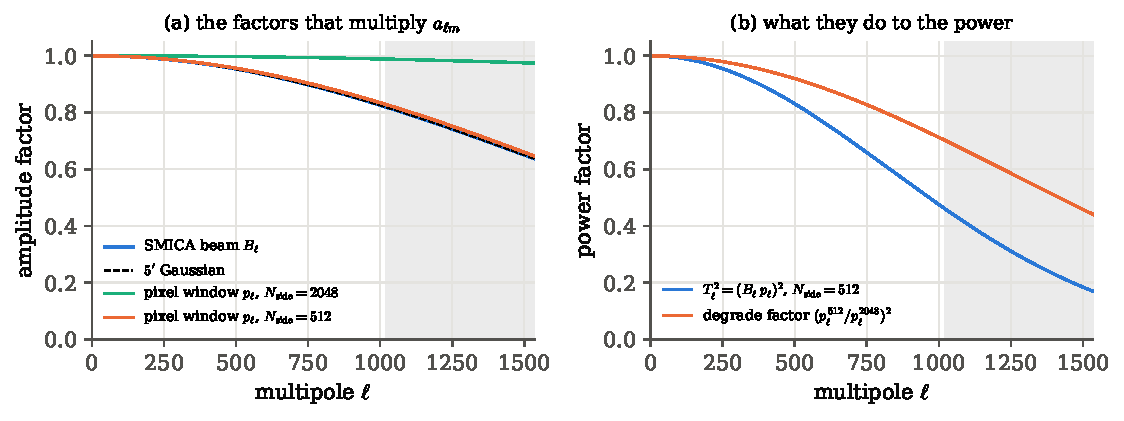
\includegraphics[width=12cm]{figures/ch13/transfer.pdf}
\caption{(a) The factors that multiply each $a_{\ell m}$ of the map: the SMICA effective beam (blue, on top
of a $5'$ Gaussian, dashed), and the pixel windows of the downloaded resolution (green) and of the working
resolution (orange). (b) Their effect on the power: the squared transfer function of the degraded map
(blue) and the squared ratio of pixel windows that the degrade applies (orange). Multipoles above
$\ell=1019$ (grey) are not analysed.}
\label{13a:fig:transfer}
\end{figure}

\paragraph{The holes have to be filled first.} One more step is needed before the transform, and it is
easy to miss. The SMICA map is not zero inside the mask; it contains the residual emission of the Galaxy and of
bright sources, which the mask exists to hide. In the full-mission map the largest value inside the holes
is $\TwelveAHoleMaxFull\,\mu$K, against $\TwelveAKeptMaxFull\,\mu$K in the kept sky. Truncating a map at
$\ell=1535$ is a low-pass filter, and a low-pass filter applied to a sharp spike produces ripples around it
(the Gibbs phenomenon of Fourier series): a hot point source of a few thousand $\mu$K would spread rings of
tens of $\mu$K into the kept pixels around its hole. So before the transform we replace the pixels inside the
mask by the inpainted CMB that \textit{Planck} provides. Those pixels stay masked in everything that follows;
the inpainting only guarantees that what is hidden in them is no brighter than the CMB, so that the band
limit cannot carry it out of the holes.

\paragraph{Example: the mask at the lower resolution.} The common mask is a 0/1 map at $N_{\rm side}=2048$
that keeps a fraction $\TwelveAFskyMaskFull$ of the sky. Each pixel at $N_{\rm side}=512$ contains
$(2048/512)^2=16$ small pixels. We keep a large pixel only if all 16 are kept; a pixel that is partly
in a hole is discarded, so a hole can only grow. The kept fraction drops to $\TwelveAFskyMaskFive$: the
holes grow by at most one large pixel ($6.9'$) along their edges.

\pyfile[firstline=33,lastline=56]{code/ch13/01_planck_data.py}{The harmonic degrade: fill the holes, transform,
swap the pixel windows, synthesise}

\noindent The loop reads each map (\texttt{full}, \texttt{hm1}, \texttt{hm2}) and converts it from K to
$\mu$K. The two lines before the transform record the largest values inside and outside the holes and
then overwrite the holes with the inpainted CMB. \pyname{hp.map2alm} computes the $a_{\ell m}$ up to
$\ell=3071$, \pyname{hp.resize_alm} keeps those up to $\ell=1535$, \pyname{hp.almxfl} multiplies them by
$p^{(512)}_\ell/p^{(2048)}_\ell$ as in \eqref{13a:eq:degrade}, and \pyname{hp.alm2map} synthesises the new map. The
whole preparation took $\TwelveAPrepSeconds$\,s; the $3.4$\,GB of downloads were then moved out of the
working directory, and the degraded maps occupy $13$\,MB each.

The full analysis does none of this: \textit{Planck} measures its spectrum at $N_{\rm side}=2048$ from the
frequency maps, not from SMICA, up to $\ell=2508$. Our reduction to $N_{\rm side}=512$ and $\ell<1020$ costs the
damping tail. The number of independent modes in a map grows as $\ell_{\max}^2$, so cutting at $1019$ instead of $2508$
keeps $(1019/2508)^2\approx17\%$ of them, and discards about four fifths of the modes \textit{Planck} analyses (fewer in
terms of information, since the noise and the foregrounds grow with $\ell$).
\section{The mask: which sky to trust, and how to let go of the rest}
\label{13a:sec:mask}

In \cref{8b:sec:apodisation} we met the trade that every mask forces on us. A mask with sharp edges keeps
every observed pixel at full weight, but its window spectrum falls slowly, so the coupling matrix carries
power from the acoustic peaks into multipoles far away; a field of small holes was the worst case, with a
leakage nearly flat in $\ell$. Tapering the edges, \emph{apodisation}, cleans the kernel by orders of
magnitude, and pays for it in modes: the effective sky fraction $\fsky w_2^2/w_4$ drops (in the example of
that section, from $802$ modes to $600$ in one bin). Those masks were caps and bands of our own design. The
\textit{Planck} common mask was designed by people who wanted to hide our Galaxy and every bright source
in the sky, and its geometry is whatever the sky made it.

\paragraph{What the mask looks like.} The common temperature mask at $N_{\rm side}=512$ keeps a fraction
$\TwelveAFskyBin$ of the sky (\cref{13a:fig:masks}a). The masked region has two very different parts. A broad
band along the Galactic plane, wider towards the Galactic centre, hides the dust, synchrotron and free-free
emission of the Milky Way. Scattered over the rest of the sky are thousands of small holes, each hiding a
radio or infrared source bright enough to be detected on its own.

\paragraph{The question.} How should each kind of hole be tapered? A wide taper around the Galactic band
costs little sky in proportion and cleans a long edge. A wide taper around each of thousands of small holes
might cost a great deal. To taper them differently we first have to tell them apart.

\subsection{Telling the holes apart}
\label{13a:sec:holes}

A \newterm{hole} is a connected set of masked pixels \unpack{masked pixels that can be joined by steps between
neighbouring masked pixels, without crossing a kept one}. On the HEALPix grid every pixel has eight
neighbours (four sharing an edge, four sharing a corner), which \pyname{hp.get_all_neighbours} lists. So the
holes are the connected components of a graph whose nodes are the masked pixels and whose links join
masked neighbours, the same idea as the clusters of \cref{ch:12}. We find them with
\pyname{scipy.sparse.csgraph.connected_components}, then measure each hole's area as its number of pixels
times the pixel area. A hole larger than $20\,\mathrm{deg}^2$ is \emph{Galactic}, the rest are
\emph{point-source holes}.

\paragraph{Example: what $20\,\mathrm{deg}^2$ means in pixels.} The sky has $41\,253\,\mathrm{deg}^2$, so at $N_{\rm side}=512$ one
pixel covers $41\,253/3\,145\,728=0.0131\,\mathrm{deg}^2$, a square of $6.9'$ on a side. A hole of $20\,\mathrm{deg}^2$ is about
$1500$ pixels, a disc of radius $2.5^\circ$. A point-source hole is a disc of a few tens of arcminutes, so
tens of pixels: the two populations are separated by two orders of magnitude, and the threshold does not
need to be chosen carefully.

The result: $\TwelveAHoles$ holes, of which $\TwelveAHolesBig$ are larger than $20\,\mathrm{deg}^2$. The Galactic holes
alone keep a fraction $\TwelveAFskyGal$ of the sky; the point-source holes alone remove a fraction
$\TwelveAFskyPS$. Together they keep $\TwelveAFskyBin=\TwelveAFskyGal-\TwelveAFskyPS$, where the source holes that
sit inside the Galactic band are not counted twice.

\subsection{Two tapers}
\label{13a:sec:taper}

\textit{Planck} apodises its Galactic masks with a Gaussian of $4.71^\circ$ FWHM ($\sigma=2^\circ$) and its
point-source masks with one of $30'$ FWHM, and multiplies the two \cite[§3.2.2]{Planck2018V}. The
apodisation is computed from the distance of each pixel to the nearest mask border, which guarantees that the
window is zero inside every hole. We follow the same logic with the cosine taper of
\cref{8b:sec:apodisation}: for a kept pixel at angular distance $d$ from the nearest hole of a given kind,
\begin{equation}
  W(d)=\begin{cases}\tfrac12\bigl(1-\cos(\pi d/\theta_{\rm ap})\bigr), & d<\theta_{\rm ap},\\[2pt] 1, & d\ge\theta_{\rm ap},\end{cases}
  \label{13a:eq:taper}
\end{equation}
with $\theta_{\rm ap}=2^\circ$ for the Galactic holes and $\theta_{\rm ap}=0.5^\circ$ for the source holes, and the
window of the analysis is the product of the two tapered masks (\cref{13a:fig:taper}). The window rises
smoothly from $0$ at the edge, through $\tfrac12$ at $d=\theta_{\rm ap}/2$, to $1$, with zero slope at both ends.

\begin{figure}[htbp]
\centering
\begin{tikzpicture}
\begin{axis}[width=10cm,height=4.6cm,xmin=-0.3,xmax=2.6,ymin=-0.05,ymax=1.12,
  xlabel={angular distance $d$ from the edge of the hole [deg]},ylabel={window $W(d)$},
  legend style={font=\footnotesize,at={(0.5,1.03)},anchor=south,legend cell align=left},
  tick label style={font=\footnotesize},label style={font=\small}]
  \fill[black!8] (axis cs:-0.3,-0.05) rectangle (axis cs:0,1.12);
  \addplot[very thick,bdryred,domain=0:0.5,samples=60] {0.5*(1-cos(deg(pi*x/0.5)))};
  \addlegendentry{point-source hole, $\theta_{\rm ap}=0.5^\circ$}
  \addplot[very thick,formblue,domain=0:2,samples=120] {0.5*(1-cos(deg(pi*x/2)))};
  \addlegendentry{Galactic hole, $\theta_{\rm ap}=2^\circ$}
  \addplot[very thick,bdryred,domain=0.5:2.6,forget plot] {1};
  \addplot[very thick,formblue,domain=2:2.6,forget plot] {1};
  \addplot[thick,black,domain=-0.3:0,forget plot] {0};
  \node[font=\footnotesize,anchor=west] at (axis cs:-0.28,0.55) {hole};
  \draw[dashed,softgray] (axis cs:0.25,0) -- (axis cs:0.25,0.5);
  \draw[dashed,softgray] (axis cs:1,0) -- (axis cs:1,0.5);
\end{axis}
\end{tikzpicture}
\caption{The two tapers of \eqref{13a:eq:taper}. Inside a hole (grey) the window is zero. Moving away from the
edge it rises as half a cosine, reaching one half at half the taper width (dashed) and one at the full
width: within $0.5^\circ$ of a point source (red), within $2^\circ$ of the Galactic band (blue).}
\label{13a:fig:taper}
\end{figure}

\paragraph{Why not one taper for all?} Take the wider taper and put it around every source. The ring
between the edge of a small hole and a distance of $2^\circ$ has an area of nearly $\pi(2^\circ)^2=12.6\,\mathrm{deg}^2$, and there
are about $3300$ such holes:
\[
  3300\times12.6\,\mathrm{deg}^2\approx41\,500\,\mathrm{deg}^2,
\]
the whole sky. The rings overlap, so the real loss is smaller, but most of the sky would sit at reduced
weight. With $0.5^\circ$ the same count gives $3300\times\pi\times0.25\,\mathrm{deg}^2\approx2600\,\mathrm{deg}^2$, about $6\%$ of the
sky, and in fact less, because inside each ring the window is on average one half. The Galactic band is one
long edge, and a $2^\circ$ taper along it costs a thin strip. So the widths are set by geometry: wide where
there is a little edge, narrow where there is a lot of it. \textit{Planck} reports the same rule of thumb:
its large Galactic apodisation reduces the effective sky fraction by about $10\%$ \cite[§3.2.2]{Planck2018V}.

\paragraph{Example: what the taper costs us.} The moments of the window
(\cref{8b:sec:masks}: $w_i$ is the average of $W^i$ over the pixels where $W>0$) are
$\fsky=\TwelveAFskyMain$ and $w_2=\TwelveAWtwoMain$, so the mean of $W^2$ over the whole sky is
$\fsky w_2=\TwelveAFwtwo$. The effective sky fraction that counts modes \eqref{8b:eq:hivon-nu} is
$\fsky w_2^2/w_4=\TwelveAFskyEffMain$, against $\TwelveAFskyEffBin$ for the binary mask. Where the error is
cosmic variance, it scales as one over the square root of the number of modes, so the taper makes the
error bars larger by
\[
  \sqrt{\TwelveAFskyEffBin/\TwelveAFskyEffMain}\approx1.05,
\]
five per cent. What it buys is visible in \cref{13a:sec:bandpowers}: without it, the correction for mode
coupling has to undo leakage of ten per cent and more.

\begin{figure}[htbp]
\centering
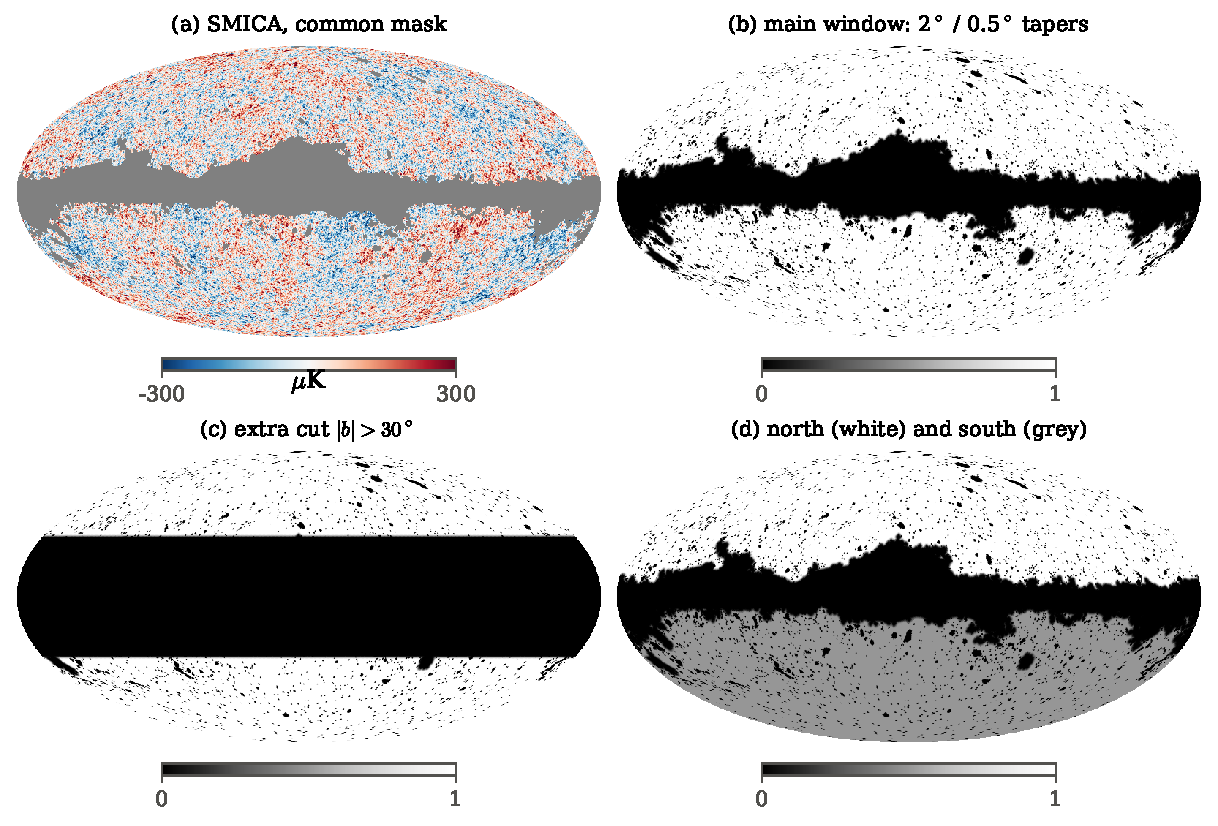
\includegraphics[width=12.4cm]{figures/ch13/masks.pdf}
\caption{(a) The degraded SMICA map outside the common mask (grey), in Galactic coordinates. (b) The window
of the analysis: the common mask with its Galactic holes tapered over $2^\circ$ and its point-source holes over
$0.5^\circ$. (c) The same window with everything at $|b|<30^\circ$ removed. (d) The northern (white) and southern
(grey) Galactic hemispheres of the window. Panels (c) and (d) are used only by the checks.}
\label{13a:fig:masks}
\end{figure}

\begin{figure}[htbp]
\centering
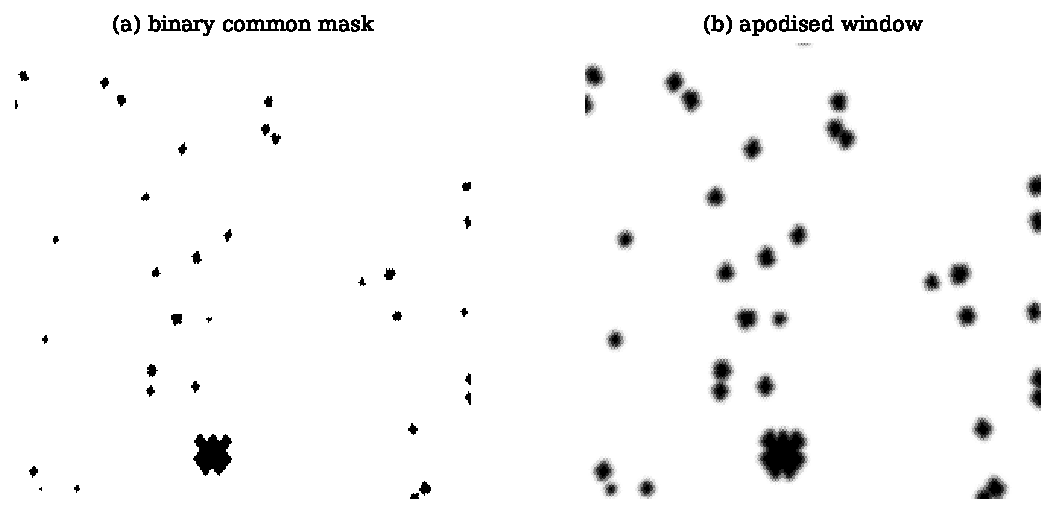
\includegraphics[width=11cm]{figures/ch13/mask_zoom.pdf}
\caption{A $20^\circ$ patch at high Galactic latitude, centred on $(l,b)=(-60^\circ,45^\circ)$. (a) The binary common
mask: a scatter of point-source holes. (b) The window: each hole is now surrounded by a grey ring where the
weight rises from zero to one over $0.5^\circ$.}
\label{13a:fig:maskzoom}
\end{figure}

\subsection{Four more windows, for the checks}
\label{13a:sec:windows}

A real analysis does not trust a spectrum measured through one window. If the map outside the mask is a
Gaussian isotropic CMB, the spectrum must not depend on which part of that sky we use, up to the scatter
that using less sky brings. So we build four more windows, each designed to expose one of the explanations
listed in \cref{13a:sec:question} (\cref{13a:fig:masks}c,d).
\begin{itemize}[itemsep=2pt]
  \item The \emph{binary} common mask, with no taper ($\fsky=\TwelveAFskyBin$). Same sky, different weights: a
        difference tests the correction for mode coupling.
  \item The main window times a cut $|b|>30^\circ$, with a $2^\circ$ cosine edge ($\fsky=\TwelveAFskyCut$). Galactic
        residuals would be stronger in the main window, which goes closer to the plane.
  \item The main window restricted to the northern or to the southern Galactic hemisphere
        ($\fsky=\TwelveAFskyNorth$ and $\TwelveAFskySouth$). A statistically isotropic sky gives the same spectrum
        in both, up to the scatter.
\end{itemize}

\paragraph{The coupling matrices.} For each window we compute the spectrum $\mathcal W_\ell$ of the window with
\pyname{hp.anafast} and the coupling matrix $M_{\ell\ell'}$ of \eqref{8b:eq:Mdef} with the Wigner-$3j$ code of
\cref{8b:sec:coupling-code}, imported from \texttt{code/ch08/lib\_masks.py}. We compute it up to $\ell=1199$,
not just to the last multipole we report, $1019$: a true multipole slightly above $1019$ leaks into our last
bins, and the correction can remove that leakage only if the matrix knows about it. Each matrix is
$1200\times1200$ and is cached in \texttt{data/ch13/}.

\pyfile[firstline=30,lastline=43]{code/ch13/02_mask.py}{Splitting the holes, tapering each kind, and the four
windows for the checks}

\noindent \pyname{lp.mask_components} returns two 0/1 masks, one with only the Galactic holes and one with only the
point-source holes. \pyname{lp.apodise} computes, for every kept pixel, the angle to the nearest masked
pixel (a nearest-neighbour search on the unit vectors of the pixel centres, with \pyname{scipy.spatial.cKDTree})
and applies \eqref{13a:eq:taper}. The latitude cuts use the same cosine edge, as a function of Galactic latitude
$b$ instead of the distance to a hole.

\textit{Planck}'s own likelihood uses a different mask at each frequency (keeping $66\%$, $57\%$ and $47\%$
of the sky at $100$, $143$ and $217$\,GHz) with the point-source holes of each channel
\cite[§3.2.2, Fig.~29]{Planck2018V}; we use the single common mask of the SMICA map, which keeps more sky
($\TwelveAFskyMain$) because SMICA has already removed most of the Galactic emission. The cost of the
substitution is that our spectrum is more exposed to any residual of SMICA's foreground cleaning near the
plane, which is exactly what the $|b|>30^\circ$ check is for.
\section{From the map to bandpowers, one correction at a time}
\label{13a:sec:bandpowers}

In \cref{8b:sec:naive,8b:sec:master} three recipes for undoing a mask were tried on simulated skies.
Dividing the pseudo-spectrum by the sky fraction was biased wherever the spectrum had structure, because
the mask moves power between multipoles. Inverting the coupling matrix multipole by multipole was exact
but noisy and, for a small patch, impossible. Inverting it between bins, the MASTER recipe, was unbiased
for any spectrum that is flat inside each bin. On simulations we could see this because we knew the
spectrum we had put in. On the real sky we do not, so we do the next best thing: apply the corrections one at a
time and watch what each does to the numbers, with \textit{Planck}'s published spectrum as a reference
line (\cref{13a:fig:steps}). Before any of that, two small things must be removed from the map, and the
spectrum must be computed in a way that has no noise bias.

\subsection{The monopole and the dipole}
\label{13a:sec:monodipole}

The SMICA map has had the monopole of the CMB (its mean temperature) and the large dipole caused by our motion
removed. What remains of $\ell=0$ and $\ell=1$ is an arbitrary offset and a residual of that subtraction,
neither of which is part of the anisotropy we model. On the full sky they would sit in $\ell=0,1$ and
never touch the multipoles we analyse. Behind a mask they do: $Y_{00}$ and $Y_{1m}$ are not orthogonal to
the higher harmonics over the cut sky, so a pure dipole on the kept pixels has pseudo-coefficients at every
$\ell$ (the leakage of \cref{8b:sec:leakage}). So we fit $c+\bm d\cdot\hat{\bm n}_p$ to the kept pixels
by least squares, four numbers ($c$ and the three components of $\bm d$), and subtract the fit from the whole map.
The fit gives $c=\TwelveAMono\,\mu$K and $|\bm d|=\TwelveADip\,\mu$K, small next to the $100\,\mu$K
fluctuations of the map. Because a mask breaks the orthogonality, this fit also absorbs the small part of the
real CMB anisotropy that happens to look like a dipole on the kept sky; it is a few $\mu$K, and it affects
mostly the buffer bin $2\le\ell<30$ that we do not report.

\subsection{Two halves, one sky}
\label{13a:sec:cross}

The half-mission maps of \cref{13a:sec:question} let us avoid the noise bias altogether. Recall
\eqref{8a:eq:cross}: if the two maps have coefficients $d^{(i)}_{\ell m}=T_\ell\alm+n^{(i)}_{\ell m}$ with
independent noise, the cross-spectrum
$\widehat C^{\,12}_\ell=\frac1{2\ell+1}\sum_m{\rm Re}\,d^{(1)}_{\ell m}d^{(2)*}_{\ell m}$ has mean $T_\ell^2\Cell$:
the noise of one half has nothing to multiply in the other, so it averages away instead of adding power.
Behind a mask the same holds for the pseudo-spectra, since the mask multiplies both maps by the same $W$.

The two halves give a second map for free. Their half-difference $(\text{hm1}-\text{hm2})/2$ contains no sky,
since the sky is the same in both, and its noise has the same level as the noise in their average
$(\text{hm1}+\text{hm2})/2$. It is a \newterm{null map}: a map of what the noise looks like. The three
spectra are tied by an identity. Write $a$ and $b$ for the masked coefficients of the two halves at
some $(\ell,m)$:
\begin{align}
  \Bigl|\frac{a+b}2\Bigr|^2-\Bigl|\frac{a-b}2\Bigr|^2
  &\eqby{1}\frac{|a|^2+|b|^2+2{\rm Re}\,ab^*}4-\frac{|a|^2+|b|^2-2{\rm Re}\,ab^*}4
  \eqby{2}{\rm Re}\,ab^* ,
  \label{13a:eq:cross-identity}
\end{align}
\begin{explain}
  \item $|a\pm b|^2=(a\pm b)(a^*\pm b^*)=|a|^2+|b|^2\pm(ab^*+a^*b)$, and $ab^*+a^*b=2{\rm Re}\,ab^*$.
  \item The squared moduli cancel.
\end{explain}
Averaging over $m$: the spectrum of the average map minus the spectrum of the half-difference is exactly the
cross-spectrum. The SMICA full-mission map is not exactly the average of the two halves (the halves
are separated with their own weights), so on the data the identity holds only approximately, and how well it
holds is one of the checks of \cref{13a:sec:checks}.

\subsection{\textit{Planck}'s bins}
\label{13a:sec:bins}

To compare our spectrum with \textit{Planck}'s we must bin exactly as \textit{Planck} bins. The published
binned spectrum uses bins of $\Delta\ell=30$ starting at $\ell=30$, and inside each bin it weights $\Cell$ by
$\ell(\ell+1)$ \cite[(22)]{Planck2018V}:
\begin{equation}
  C_b=\sum_{\ell\in b}w_{b\ell}\Cell,\qquad w_{b\ell}=\frac{\ell(\ell+1)}{\sum_{\ell'\in b}\ell'(\ell'+1)},\qquad
  \ell_b^{\rm eff}=\sum_{\ell\in b}w_{b\ell}\,\ell,\qquad
  D_b=\frac{\ell_b^{\rm eff}(\ell_b^{\rm eff}+1)}{2\pi}\,C_b .
  \label{13a:eq:planck-bin}
\end{equation}
The weight $\ell(\ell+1)$ is there because $D_\ell=\ell(\ell+1)\Cell/2\pi$ varies slowly across a bin while $\Cell$
falls steeply: weighting $\Cell$ by $\ell(\ell+1)$ averages the slowly varying quantity. The file quotes $D_b$ at
the multipole $\ell_b^{\rm eff}$.

In the notation of the MASTER estimator (\cref{8b:sec:binning}), binning is a matrix $P_{b\ell}$ that turns a
spectrum into bandpowers, and $Q_{\ell b}$ is a matrix that spreads a bandpower back over the multipoles of its
bin. Reading them off \eqref{13a:eq:planck-bin},
\begin{equation}
  P_{b\ell}=\frac{\ell_b^{\rm eff}(\ell_b^{\rm eff}+1)}{2\pi}\,w_{b\ell},\qquad
  Q_{\ell b}=\frac{2\pi}{\ell_b^{\rm eff}(\ell_b^{\rm eff}+1)}\quad(\ell\in b),
  \label{13a:eq:PQ}
\end{equation}
and both are zero for $\ell$ outside bin $b$. $Q$ is the spectrum that the MASTER recipe assumes inside each bin: a
$\Cell$ that is constant across the bin, at the value whose $D$ at $\ell_b^{\rm eff}$ is the bandpower. Binning that
spectrum must give the bandpower back:
\begin{align}
  \sum_\ell P_{b\ell}Q_{\ell b'}
  &\eqby{1}\delta_{bb'}\sum_{\ell\in b}\frac{\ell_b^{\rm eff}(\ell_b^{\rm eff}+1)}{2\pi}\,w_{b\ell}\,
     \frac{2\pi}{\ell_b^{\rm eff}(\ell_b^{\rm eff}+1)}
   \eqby{2}\delta_{bb'}\sum_{\ell\in b}w_{b\ell}
   \eqby{3}\delta_{bb'} .
\end{align}
\begin{explain}
  \item $P_{b\ell}$ is zero unless $\ell\in b$ and $Q_{\ell b'}$ is zero unless $\ell\in b'$; bins do not overlap,
        so the product vanishes unless $b=b'$.
  \item The two prefactors cancel.
  \item The weights of a bin sum to one by construction.
\end{explain}
So $PQ=\Id$, the property the derivation of \eqref{8b:eq:master-derivation} needs.

\paragraph{Example: the first bin.} For $30\le\ell\le59$,
$\ell^{\rm eff}=\sum\ell^2(\ell+1)/\sum\ell(\ell+1)=\TwelveABinFirstLeff$; the \textit{Planck} file quotes $47.711$, and our
binning code reproduces every $\ell_b^{\rm eff}$ in the file to better than one part in $10^5$ (the largest difference is \TwelveALeffCheck). Now take the fiducial
spectrum and bin it. The plain average of $D_\ell$ over the bin is $\TwelveABinFirstDmean\,\mu{\rm K}^2$, and $D_\ell$ at
$\ell=48$ is $\TwelveABinFirstDat\,\mu{\rm K}^2$, but \eqref{13a:eq:planck-bin} gives $D_b=\TwelveABinFirstDb\,\mu{\rm K}^2$. A
bandpower is neither the spectrum at $\ell^{\rm eff}$ nor its average. To see why, take a $D_\ell=D$ that is flat
across the bin, so that $\Cell=2\pi D/\ell(\ell+1)$:
\begin{align}
  D_b
  &\eqby{1}\frac{\ell^{\rm eff}(\ell^{\rm eff}+1)}{2\pi}\sum_{\ell\in b}\frac{\ell(\ell+1)}{\sum_{\ell'\in b}\ell'(\ell'+1)}\,
     \frac{2\pi D}{\ell(\ell+1)}
   \eqby{2}\frac{\ell^{\rm eff}(\ell^{\rm eff}+1)\,\Delta\ell}{\sum_{\ell'\in b}\ell'(\ell'+1)}\,D
   \eqby{3}\frac{\ell^{\rm eff}(\ell^{\rm eff}+1)}{\overline{\ell(\ell+1)}}\,D .
\end{align}
\begin{explain}
  \item \eqref{13a:eq:planck-bin} with $\Cell=2\pi D/\ell(\ell+1)$.
  \item The factors $\ell(\ell+1)$ and $2\pi$ cancel, and the sum of $1$ over the bin is its width $\Delta\ell$.
  \item $\overline{\ell(\ell+1)}$ is the plain average of $\ell(\ell+1)$ over the bin.
\end{explain}
In the first bin the factor is $\TwelveABinFirstLL/\TwelveABinFirstLLmean=\TwelveABinFirstFactor$: the effective multipole is a weighted
mean of $\ell$, and squaring a mean is not the mean of the squares. In the last bin, $990\le\ell\le1019$, the
same factor is $\TwelveABinLastFactor$, because the bin is narrow compared with its $\ell$. The lesson is a rule we will use
repeatedly: a theory curve is compared with bandpowers only after it has been passed through \emph{the same}
binning (and, below, the same window).

We add a buffer bin $2\le\ell<30$ below the reported range and six bins $1020\le\ell<1200$ above it. They are
solved for together with the reported bins, so that the power at those multipoles, which the mask spreads into
our range, is accounted for, and then they are discarded. We report $\TwelveANbins$ bins, $\TwelveALlo\le\ell\le\TwelveALhi$.

\begin{figure}[htbp]
\centering
\begin{tikzpicture}[x=0.0076cm,y=1cm]
  \draw[->,thick] (0,0) -- (1250,0) node[right,font=\small] {$\ell$};
  \fill[black!12] (2,0.05) rectangle (30,0.55);
  \fill[formblue!20] (30,0.05) rectangle (1020,0.55);
  \fill[black!12] (1020,0.05) rectangle (1200,0.55);
  \foreach \e in {30,60,...,1020}{\draw[formblue!70!black] (\e,0.05) -- (\e,0.55);}
  \foreach \e in {1050,1080,...,1200}{\draw[black!50] (\e,0.05) -- (\e,0.55);}
  \foreach \e in {0,200,400,600,800,1000,1200}{\draw (\e,0) -- (\e,-0.08) node[below,font=\footnotesize] {\e};}
  \node[font=\footnotesize,align=center,anchor=south] at (16,0.6) {buffer};
  \node[font=\footnotesize,anchor=south] at (525,0.6) {33 reported bins, $\Delta\ell=30$};
  \node[font=\footnotesize,anchor=south] at (1110,0.6) {buffer};
  \draw[bdryred,thick] (0,-0.75) -- (1535,-0.75);
  \node[font=\footnotesize,bdryred,anchor=west] at (0,-1.05) {multipoles in the degraded map, $\ell\le1535$};
  \draw[tangentgreen!70!black,thick] (0,-1.45) -- (1199,-1.45);
  \node[font=\footnotesize,tangentgreen!50!black,anchor=west] at (0,-1.75) {coupling matrix $M_{\ell\ell'}$, $\ell\le1199$};
\end{tikzpicture}
\caption{The bins. Thirty-three bins of thirty multipoles (blue) are reported, exactly \textit{Planck}'s binning
between $\ell=30$ and $1019$. Below and above them, buffer bins (grey) absorb the power that the mask moves into
the reported range from outside it; they are solved for and discarded. The degraded map holds multipoles up to
$1535$; the coupling matrix is computed up to $1199$.}
\label{13a:fig:bins}
\end{figure}

\subsection{MASTER with our own coupling matrix}
\label{13a:sec:master-real}

With the coupling matrix $M$ of the window (\cref{13a:sec:windows}) and the squared transfer function
$T_\ell^2=(B_\ell p_\ell)^2$ of \cref{13a:sec:files}, the binned master equation
\eqref{8b:eq:master-derivation} \srcref{Hivon}{(20)--(26)} reads, for the cross-spectrum (no noise term to subtract, and no time-domain
filtering, $F_\ell=1$),
\begin{equation}
  \langle P\widetilde C^{\,12}\rangle=K\,D,\qquad K_{bb'}=\sum_{\ell\ell'}P_{b\ell}M_{\ell\ell'}T^2_{\ell'}Q_{\ell'b'},
  \qquad \widehat D_b=\sum_{b'}K^{-1}_{bb'}\sum_\ell P_{b'\ell}\widetilde C^{\,12}_\ell .
  \label{13a:eq:master}
\end{equation}
$K$ is $40\times40$ (the $33$ reported bins and the $7$ buffer bins), and it is inverted once. As derived in
\eqref{8b:eq:bpw}, the mean of $\widehat D_b$ for the true spectrum is
\begin{equation}
  \langle\widehat D_b\rangle=\sum_\ell\mathcal F_{b\ell}\Cell,\qquad
  \mathcal F_{b\ell}=\sum_{b'}K^{-1}_{bb'}\sum_{\ell'}P_{b'\ell'}M_{\ell'\ell}T_\ell^2 ,
  \label{13a:eq:bpw}
\end{equation}
the \newterm{bandpower window functions}. They are the honest way to put a theory on the plot: a spectrum that
is not flat inside each bin is turned into bandpowers by $\mathcal F$, not by $P$. NaMaster, the public code that implements MASTER for any mask, writes
the same two equations, the binned coupling matrix and the filter that must be applied to any theory before
it is compared with the data \cite[(16)--(18)]{Alonso2019}.

\begin{figure}[htbp]
\centering
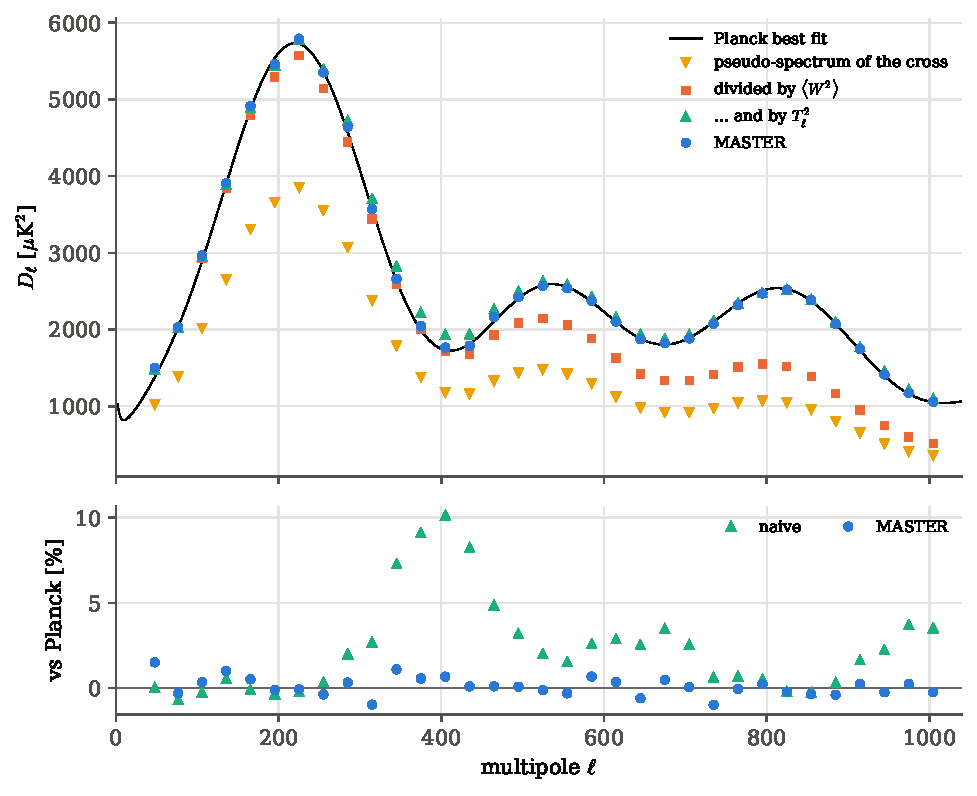
\includegraphics[width=10.4cm]{figures/ch13/steps.pdf}
\caption{The SMICA half-mission cross-spectrum, binned in \textit{Planck}'s bins, after each correction. Top:
the binned pseudo-spectrum (yellow triangles); divided by the mean of $W^2$ (orange squares); then also by
$T_\ell^2$ (green triangles, the naive estimator); and the MASTER bandpowers (blue). The black line is the
\textit{Planck} best fit. Bottom: the naive and the MASTER bandpowers relative to \textit{Planck}'s published
bandpowers.}
\label{13a:fig:steps}
\end{figure}

\paragraph{What each step does, on the data.} \Cref{13a:fig:steps} follows the cross-spectrum through the
corrections.
\begin{enumerate}[itemsep=2pt,leftmargin=1.5em]
  \item \emph{The pseudo-spectrum} is low everywhere. In the first bin it is $\TwelveARawFirst\,\mu{\rm K}^2$,
        against $\TwelveAPlFirst$ in \textit{Planck}'s spectrum.
  \item \emph{Dividing by the mean of $W^2$} over the sky, $\fsky w_2=\TwelveAFwtwo$, fixes the low multipoles
        ($\TwelveARawFirst/\TwelveAFwtwo\approx1478$), but the high ones stay low, and more so the higher $\ell$.
  \item \emph{Dividing by $T_\ell^2$} undoes the beam and the pixels; at $\ell=1019$ that is a factor
        $1/\TwelveATsqTen$. The result is the naive estimator \eqref{8b:eq:naive}, and it is off by up to
        $\TwelveANaiveMaxDev\%$, with a characteristic pattern: too high in the troughs, especially the first one
        near $\ell=400$, nearly right at the peaks.
  \item \emph{MASTER} removes the pattern. Its bandpowers differ from \textit{Planck}'s by at most
        $\TwelveAMasterMaxDev\%$, $\TwelveAMasterRms\%$ in the root mean square.
\end{enumerate}

\paragraph{Why the naive estimator fails in the troughs.} Dividing by $\fsky w_2$ assumes that the mask
removes a fixed share of the power at each multipole and moves none of it: $M_{\ell\ell'}=\fsky w_2\,\delta_{\ell\ell'}$.
The true coupling matrix has a narrow core around $\ell'=\ell$, set by the size of the large sky
regions, and a broad low floor that comes from the thousands of small holes, whose window spectrum is
nearly flat (\cref{8b:sec:apodisation}). The floor moves a small fraction of every multipole's power to
multipoles far away. At a peak the power that leaves and the power that arrives nearly balance. In the trough
at $\ell\approx400$, where $D_\ell\approx1750\,\mu{\rm K}^2$, the arriving share of the first peak, where
$D_\ell\approx5800\,\mu{\rm K}^2$, is not balanced by the little that leaves, so the trough fills up by about a tenth.
The $0.5^\circ$ taper of the source holes weakens the floor but cannot remove it, because the holes themselves
are small. MASTER does not need the floor to be small; it needs it to be known, and $M$ knows it.

\paragraph{Example: the residual of MASTER, in perspective.} The bottom panel of \cref{13a:fig:steps} shows MASTER
within $\TwelveAMasterMaxDev\%$ of \textit{Planck}'s bandpowers. Is that agreement good, or suspiciously good?
Neither question can be answered yet. Both bandpowers are measurements of nearly the same sky, so they share
most of their cosmic variance, and their difference is much smaller than either one's error bar. How much
smaller is a question about the joint sampling distribution of two estimators, and it needs simulated skies
(\cref{13a:sec:sims,13a:sec:why}).

\pyfile[firstline=49,lastline=64]{code/ch13/03_bandpowers.py}{The spectra of every window: pseudo-spectra of the
halves, their cross, their half-difference, and the MASTER correction}

\noindent For each window the loop loads the cached coupling matrix and builds the MASTER operator
(\pyname{lp.Master}: it forms $K$ of \eqref{13a:eq:master} once and inverts it). \pyname{lp.pseudo_cl} multiplies each map
by the window and transforms it. From the three sets of coefficients come the cross-spectrum of the halves, the
spectrum of their half-difference and the auto-spectrum of the full map, each corrected by the same operator.
\pyname{mst.window()} returns the bandpower windows $\mathcal F_{b\ell}$ of \eqref{13a:eq:bpw}, which the
comparison with theory uses.
\section{How much would the bandpowers scatter? Simulated skies}
\label{13a:sec:sims}

We now have $\TwelveANbins$ numbers, one per bin, measured from one sky. Each of them is a draw from a sampling
distribution that we cannot observe: the distribution of the bandpowers over all the skies the standard model
could have produced, each seen through \textit{Planck}'s beam, pixels, noise and our mask. In \cref{ch:08}
that distribution was the research problem, and simulation was the answer: for a masked, noisy sky no formula
gives the covariance of MASTER bandpowers exactly, and the scatter of the estimator over many simulated skies
is the measurement (\cref{8b:sec:research}). Here the same machine runs for real. Two things must be decided
before it can: what noise the simulated maps carry, and how many of them we can afford.

\subsection{A noise model built from the data}
\label{13a:sec:noise}

\textit{Planck} simulates its noise end to end: the time-ordered data of every detector are simulated with the
measured noise properties, made into maps by the same map-making code, and passed through the component
separation, giving a few hundred noise realisations of each map (the FFP10 simulations). We have only the
data. But the data contain a map of their own noise: the half-difference
$d=(\text{hm1}-\text{hm2})/2$ of \cref{13a:sec:cross}, in which the sky cancels.

\paragraph{The question.} What random map, added to a simulated sky, would make a half-mission map whose noise
looks like ours? Two features of $d$ matter. Its \emph{amplitude varies over the sky}, because \textit{Planck}'s
scanning covers some regions many more times than others and the component separation weights the
frequencies differently in different places. And its \emph{power varies with scale}, because SMICA's weights
and the deconvolution of each channel's beam to the common $5'$ make the noise anything but white. A model
that captures both, and nothing more, is
\begin{equation}
  n_{\rm half}(p)=\sqrt2\,\sqrt{v(p)}\;g(p),
  \label{13a:eq:noise-model}
\end{equation}
where $v(p)$ is the local variance of $d$ relative to its mean (the map $d^2$ smoothed with a $2^\circ$ Gaussian and
divided by its average over the kept sky), and $g$ is a statistically isotropic Gaussian field whose spectrum
$N^g_\ell$ is that of $d/\sqrt v$, measured through the window and divided by the mean of $W^2$
(\cref{8b:sec:naive}), then averaged over $31$ neighbouring multipoles to remove its own scatter.

\paragraph{Where the $\sqrt2$ comes from.} Suppose the noise of each half has variance $\sigma^2$ in some
pixel, and the two halves are independent. Then
\begin{align}
  \Var(d)
  &\eqby{1}\Var\Bigl(\frac{n_1-n_2}2\Bigr)
   \eqby{2}\frac{\Var n_1+\Var n_2}4
   \eqby{3}\frac{\sigma^2}2
  \quad\Longrightarrow\quad\sigma^2=2\Var(d) .
\end{align}
\begin{explain}
  \item The sky is identical in the two halves and cancels in $d$.
  \item The variance of a sum of independent variables is the sum of the variances, and a constant factor
        comes out squared: $(1/2)^2$, with $(-1)^2=1$ for the second term.
  \item Both halves have the same noise level.
\end{explain}
So a half's noise has twice the variance of $d$, a factor $\sqrt2$ in amplitude. By the same steps, the
average of the halves, $(n_1+n_2)/2$, has variance $\sigma^2/2=\Var(d)$: the noise of the full map has the spectrum
of $d$ itself, and the noise of one half has twice that spectrum.

\paragraph{Example: how much noise is there?} Very little, at these multipoles. At $\ell=1000$ the noise power of
the full map is $\TwelveANoiseRatioK\%$ of the beamed sky power $T_\ell^2\Cell$, and the noise of a single half stays
below the beamed sky at every $\ell\le1199$ (\cref{13a:fig:noise}a). In temperature, below $\ell\approx1000$,
\textit{Planck} is limited by cosmic variance, not by its detectors, which is why the noise model can be
approximate without changing the error bars much. Where the noise is, however, varies a lot: $v$ reaches
$\TwelveAVmax$ times the mean in the worst regions (\cref{13a:fig:noise}b). Close to the mask edges $v$ is
artificially small, because the holes were filled with the same inpainted map in both halves, so $d=0$ there
and the smoothing pulls $v$ down; a floor of $\TwelveAVmin$ keeps $d/\sqrt v$ finite.

\begin{figure}[htbp]
\centering
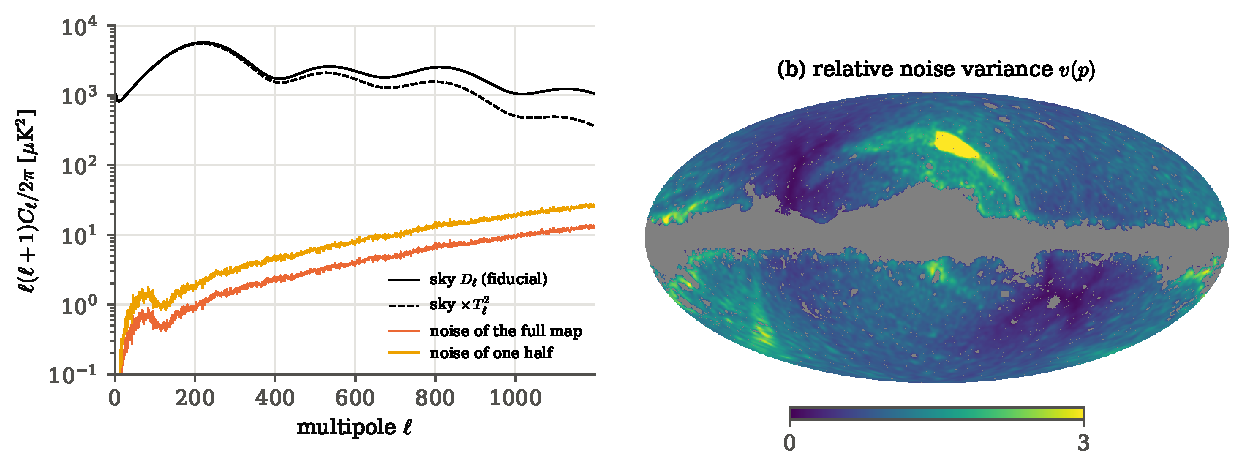
\includegraphics[width=12.4cm]{figures/ch13/noise.pdf}
\caption{(a) The fiducial sky spectrum (solid black), the same after the beam and pixel window (dashed), and
the noise spectra measured from the half-difference map: the noise of the full map (red) and of one half
(orange). Below $\ell=1200$ the sky dominates everywhere. (b) The relative noise variance $v(p)$ outside the
mask: the noise level changes by more than a factor of ten over the sky.}
\label{13a:fig:noise}
\end{figure}

What the model leaves out is equally important to state. The noise is drawn Gaussian, while residual
glitches and foreground leftovers are not. Its correlations are those of a modulated isotropic field, while
real scanning noise has stripes along the scan direction. The two halves are drawn independent, while
\textit{Planck} found small correlations between half-missions at high multipoles
\cite[§3.2.1]{Planck2018V}. And $v$ and $N^g_\ell$ were estimated from the very map whose noise they describe, so
the half-difference test of \cref{13a:sec:checks} is a consistency check of the model, not an independent test of
it.

\subsection{The simulated skies}
\label{13a:sec:simrecipe}

The rule that makes simulations useful is simple and absolute: \emph{whatever is done to the data is done to
every simulation}. The same beam, the same pixel window, the same noise model, the same five windows, the same
binning and the same MASTER operator.

\paragraph{Recipe for one simulated sky.}
\begin{enumerate}[itemsep=1pt,leftmargin=1.4em]
  \item Draw $\alm$ from the fiducial lensed spectrum $\Cell$ (CAMB at the \textit{Planck} 2018 best fit
        \cite{CAMB2000}, \cref{7b:sec:camb}), for $\ell\le1535$.
  \item Multiply by $T_\ell=B_\ell p^{(512)}_\ell$ and synthesise the sky map $s$ at $N_{\rm side}=512$.
  \item Make two half-mission maps $s+n_1$ and $s+n_2$, with $n_1,n_2$ independent draws of \eqref{13a:eq:noise-model}.
  \item For each of the five windows, compute the pseudo-coefficients of both halves, their cross-spectrum and
        the spectrum of their half-difference, and correct both with that window's MASTER operator
        \eqref{13a:eq:master}.
\end{enumerate}
The output is, for each sky and each window, $\TwelveANbins$ cross bandpowers and $\TwelveANbins$ null bandpowers.

One sky takes $\TwelveASecPerSky$\,s on four cores: three map syntheses and ten masked transforms at
$N_{\rm side}=512$. We ran $\TwelveANsimDone$ skies, in chunks of $50$ cached in \texttt{data/ch13/} so that an
interrupted run resumes where it stopped. The skies are Gaussian, while the real sky is slightly non-Gaussian
through gravitational lensing; the lensed spectrum gets the mean right, and the extra covariance that lensing
induces between multipoles is negligible at our error bars below $\ell\approx1000$.

\pyfile[firstline=95,lastline=108]{code/ch13/04_sims.py}{One simulated sky, observed and analysed like the real one}

\noindent \pyname{cs.synalm} is the Gaussian $\alm$ generator of \cref{ch:08} (\texttt{code/ch08/lib\_cmbsim.py}).
The sky map is made once and shared by the two halves; each half gets its own noise, a Gaussian field with
spectrum $N^g_\ell$ multiplied pixel by pixel by $\sqrt{2v}$. The inner loop is \cref{13a:sec:master-real} again,
line for line.

\subsection{What the simulations say}
\label{13a:sec:cov}

\paragraph{Is the estimator unbiased?} If MASTER is unbiased, the average of the simulated bandpowers must
equal the fiducial spectrum passed through the bandpower windows, $t_b=\sum_\ell\mathcal F_{b\ell}\Cell$
\eqref{13a:eq:bpw}. The question in words: if the theory were right, would an average of $n$ simulated
bandpower vectors as far from $\bm t$ as ours, or farther, be something we would reasonably expect? The average
$\bar{\bm x}$ of $n$ independent vectors with covariance $\Cmat$ has covariance $\Cmat/n$. For Gaussian vectors with
mean $\bm t$,
\begin{equation}
  \chi^2_{\rm bias}=(\bar{\bm x}-\bm t)\T\Bigl(\frac{\Cmat}{n}\Bigr)^{-1}(\bar{\bm x}-\bm t)
  =n\,(\bar{\bm x}-\bm t)\T\Cmat^{-1}(\bar{\bm x}-\bm t)
  \label{13a:eq:bias-chi2}
\end{equation}
is a $\chi^2$ with $p=\TwelveAP$ degrees of freedom: a quadratic form in a Gaussian vector, weighted by the
inverse of its own covariance, is a sum of $p$ squared independent unit Gaussians (\cref{2b:sec:chi2-quadform}).
In practice $\Cmat$ is itself estimated from the same simulations, and its inverse is multiplied by the
Hartlap factor $(n-p-2)/(n-1)=\TwelveAHartlap$ derived in \cref{8b:sec:hartlap}, which removes the bias of the
inverse of a noisy matrix.

With the exact windows, $\chi^2_{\rm bias}=\TwelveABiasChiExact$ for $\TwelveAP$ degrees of freedom, a probability
to exceed of $\TwelveABiasPteExact$: no sign of bias, at the precision of $\TwelveANsimUsed$ simulations, which
is $1/\sqrt{\TwelveANsimUsed}$ of an error bar. If instead the theory is binned with the plain operator $P$, as
if it were flat inside each bin, $\chi^2_{\rm bias}=\TwelveABiasChiNaive$ (\cref{13a:fig:cov}b). The difference
between the two theory vectors is at most $\TwelveAWinMaxPct\%$, which is $\TwelveAWinMaxSig$ of a single
bandpower's error bar: small for one sky, but the average of $\TwelveANsimUsed$ skies is twenty times more
precise and sees it. The same is true of any analysis that averages many bandpowers into a few parameters, which
is why the NaMaster authors insist on the exact windows \cite[§2.1, Fig.~10]{Alonso2019}.

\paragraph{How large are the error bars?} The square roots of the diagonal of $\Cmat$ are our error bars. Two
estimates give them a size. The cosmic variance of a bin on the \emph{full} sky, with no noise, is the
variance of the average of $\Delta\ell$ independent $\widehat D_\ell$, each of variance $2D_\ell^2/(2\ell+1)$
\eqref{7b:eq:cosmic-var}. Our error bars are larger by a factor $\TwelveAErrOverCvLow$ in the first bin,
$\TwelveAErrOverCvMid$ (median) over the first fifteen, and $\TwelveAErrOverCvHigh$ in the last. The mode
counting of \eqref{8b:eq:hivon-nu} predicts $1/\sqrt{\fsky w_2^2/w_4}=\TwelveAOneOverSqrtFeff$ where the noise is
negligible, and more where it is not. The bins in the middle of the range, where the noise is still negligible, sit about
$7\%$ above that prediction, and the first bin sits $\TwelveAErrOverCvLow/\TwelveAOneOverSqrtFeff\approx1.24$ times above it. Mode counting
with one effective sky fraction describes the covariance of a masked spectrum only to leading order. What it leaves out
(the coupling of neighbouring multipoles through the small holes, and the amplification of fluctuations when MASTER inverts the
coupling, which in the first bin is done together with the buffer bin below it) is exactly what the simulations contain.

\paragraph{Example: Knox's formula against the simulations.} In the first bin, $\ell^{\rm eff}=47.7$ and
$\Delta\ell=30$, Knox's formula with the effective sky fraction,
$\sigma(D_b)\approx\sqrt{2/[(2\ell^{\rm eff}+1)\Delta\ell\,\fsky w_2^2/w_4]}\;D_b$ (\cref{8a:sec:knox}), gives
$\TwelveAKnoxFirst\,\mu{\rm K}^2$; the simulations give $\TwelveASigFirst\,\mu{\rm K}^2$. In the last bin the
formula, which ignores the noise, gives $\TwelveAKnoxLast$ against $\TwelveASigLast$. The formula is a good
first guess, and the simulations are the answer.

\paragraph{Are neighbouring bins correlated?} The mask couples multipoles, so the bandpowers of
neighbouring bins share some of their fluctuations (\cref{8b:sec:corr}). With bins of $30$ multipoles, wide
compared with the coupling kernel's core, the correlation is weak: on average $\TwelveACorrNext$ between
neighbours, and at most $\TwelveACorrNextMin$ in magnitude in the other direction (\cref{13a:fig:cov}a).
MASTER's deconvolution tends to make neighbours slightly \emph{anti}-correlated: when it undoes the coupling, an
upward fluctuation that the mask spread into the next bin is subtracted from it.

\paragraph{How good is the covariance itself?} Every element of $\Cmat$ is estimated from $\TwelveANsimUsed$
draws. A diagonal element, a sample variance, has a relative error of $\sqrt{2/(n-1)}$
(\cref{8b:sec:cov-element-noise}); the error bar is its square root, so its relative error is half of that,
$1/\sqrt{2(n-1)}=\TwelveAMcErrSig\%$. Our error bars are uncertain by about $\TwelveAMcErrSig\%$, and the
probabilities to exceed computed below are good to a few per cent of their value.

\begin{figure}[htbp]
\centering
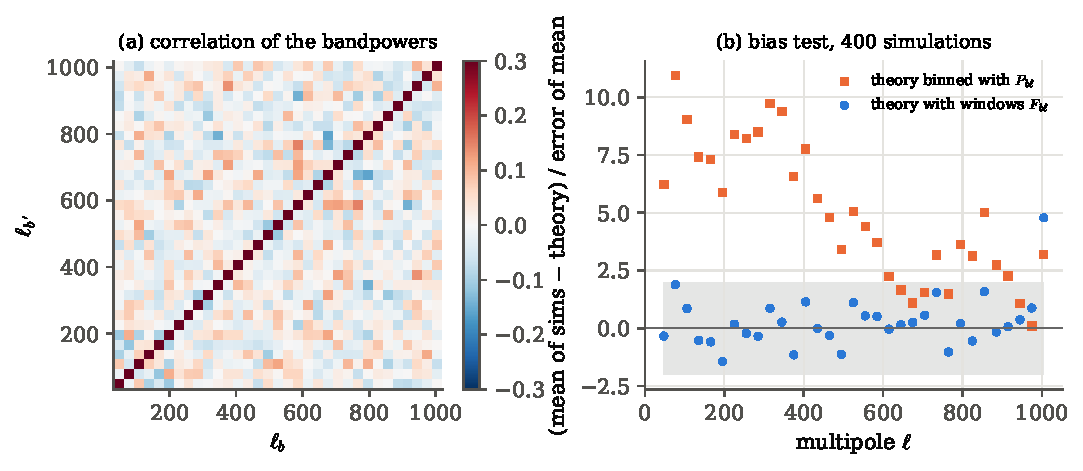
\includegraphics[width=12.4cm]{figures/ch13/covariance.pdf}
\caption{(a) The correlation matrix of the $\TwelveAP$ bandpowers from the simulations: almost diagonal, with weak
correlations between neighbours. (b) The bias test: the average of the simulated bandpowers minus the theory,
in units of the error of the average. The theory passed through the exact bandpower windows (blue) is
consistent with zero; the theory binned as if it were flat in each bin (orange) is not.}
\label{13a:fig:cov}
\end{figure}

\paragraph{How research codes get the covariance.} Here the simulations are the research instrument, not a check of a
formula. \textit{Planck}'s high-$\ell$ likelihood uses an analytic covariance instead, computed from the fiducial spectrum, the masks and a noise model,
with corrections for the point-source holes and the anisotropic noise calibrated on simulations
\cite[§3.1]{Planck2018V}. Efstathiou showed why this is possible at high $\ell$: for apodised masks the
pseudo-$\Cell$ covariance is close to an analytic expression, and the estimator is nearly as precise as the
maximum-likelihood one \cite{Efstathiou2004}. The end-to-end FFP10 simulations then validate the analytic
covariance rather than replace it. Both routes need the same thing we built: a model of the observation good
enough that simulated and real skies are statistically indistinguishable.
\section{Our spectrum against \textit{Planck}'s}
\label{13a:sec:compare}

\paragraph{Their question.} The \textit{Planck} collaboration wanted the temperature power spectrum of the CMB
over $30\le\ell\le2508$ with errors small enough that the six parameters of $\Lambda$CDM would be limited by
the sky, not by the instrument, and a likelihood that turns that spectrum into parameters without bias
\cite[§1, §3]{Planck2018V}. The binned spectrum in the file we downloaded is one product of that work: the
CMB spectrum after the foreground model has been subtracted and the frequency channels have been averaged.

\paragraph{Their setup, in plain terms.} The high-$\ell$ likelihood code of the release is called Plik. It did not use a component-separated map. It measured
cross-spectra between the half-mission maps of three frequency channels, $100$, $143$ and $217$\,GHz, each
through its own mask (keeping $66\%$, $57\%$ and $47\%$ of the sky) with apodised Galactic and point-source
holes, over a multipole range chosen per channel \cite[§3.2.1--3.2.4, Table~13]{Planck2018V}. The residual
emission of dust, of unresolved galaxies and of galaxy clusters was not masked away but \emph{modelled}: each
foreground has a spectrum with a few free amplitudes, fitted together with the cosmology. The covariance
of the spectra is computed analytically from the fiducial model, the masks and a noise model. Our setup
differs in almost every item (\cref{13a:tab:compare}), and the point of the comparison is to see whether the
two routes land on the same spectrum.

\begin{table}[htbp]
\centering\small
\begin{tabular}{@{}lll@{}}
\toprule
 & \textit{Planck} 2018 (Plik) & ours\\
\midrule
maps & $100$, $143$, $217$\,GHz half-missions & SMICA half-missions\\
resolution & $N_{\rm side}=2048$ & $N_{\rm side}=512$\\
masks & one per frequency, $47$--$66\%$ of the sky & common mask, $\TwelveAFskyMain$ of the sky\\
foregrounds & modelled, amplitudes fitted & removed by SMICA, the rest masked\\
multipoles & $30\le\ell\le2508$ & $30\le\ell\le1019$\\
covariance & analytic, validated on simulations & $\TwelveANsimUsed$ Gaussian simulations\\
binning (this file) & $\Delta\ell=30$, weights $\ell(\ell+1)$ & identical\\
\bottomrule
\end{tabular}
\caption{The two analyses compared. Only the binning is the same.}
\label{13a:tab:compare}
\end{table}

\subsection{Their key equation: a Gaussian likelihood for bandpowers}
\label{13a:sec:gauss-like}

\textit{Planck}'s high-$\ell$ likelihood is \cite[(20)]{Planck2018V}
\begin{equation}
  -\ln\Like(\params)=\tfrac12\bigl[\widehat{\bm C}-\bm C(\params)\bigr]\T\Sigma^{-1}\bigl[\widehat{\bm C}-\bm C(\params)\bigr]+\text{const},
  \label{13a:eq:plik}
\end{equation}
with $\widehat{\bm C}$ the vector of measured bandpowers, $\bm C(\params)$ the model passed through the same binning,
and $\Sigma$ their covariance. Where does it come from? Ask the likelihood's question
(\cref{3b:sec:likelihood}): for given parameters, how plausible is the fluctuation that turns the model
prediction into the bandpowers we observed? Answering it needs the sampling distribution of the bandpowers.
Each bandpower is an average over many modes, $(2\ell+1)\,\Delta\ell\,\fsky w_2^2/w_4\approx2000$ already in our
first bin, and an average of many independent pieces is close to Gaussian (the central limit theorem,
\cref{2b:sec:clt}). Hamimeche and Lewis checked how close: at high $\ell$ the Gaussian form, with a
covariance computed at the fiducial model, gives the same parameters as the exact likelihood
\cite{HamimecheLewis2008}, while at $\ell\lesssim30$, where the exact distribution is a skewed scaled $\chi^2$, it does
not (\cref{9c:sec:hl}). That is why \textit{Planck} splits its likelihood at $\ell=30$, and why we start there. With a
Gaussian sampling distribution,
\begin{align}
  p\bigl(\widehat{\bm D}\given\params\bigr)
  &\eqby{1}\frac{1}{\sqrt{(2\pi)^p\det\Cmat}}\exp\Bigl[-\tfrac12\bigl(\widehat{\bm D}-\bm t(\params)\bigr)\T\Cmat^{-1}\bigl(\widehat{\bm D}-\bm t(\params)\bigr)\Bigr],
  \nonumber\\
  -2\ln\Like(\params)
  &\eqby{2}\bigl(\widehat{\bm D}-\bm t(\params)\bigr)\T\Cmat^{-1}\bigl(\widehat{\bm D}-\bm t(\params)\bigr)+\text{const}
  \equiv\chi^2(\params)+\text{const},
  \label{13a:eq:like}
\end{align}
\begin{explain}
  \item The multivariate Gaussian density of $p$ bandpowers with mean $\bm t(\params)$, the model through the
        bandpower windows \eqref{13a:eq:bpw}, and covariance $\Cmat$ (\cref{2b:sec:mvn}).
  \item Read as a function of $\params$ with the data fixed; $\Cmat$ is held at its fiducial value, so
        $\det\Cmat$ is a constant and goes into it.
\end{explain}
This is \eqref{13a:eq:plik} in our symbols: $\widehat{\bm C}\to\widehat{\bm D}$ (we work in $D_b$), $\bm C(\params)\to\bm t(\params)$,
$\Sigma\to\Cmat$. In our analysis $\Cmat$ is the simulated covariance of \cref{13a:sec:cov} and its inverse carries the
Hartlap factor.

\subsection{What we compute}
\label{13a:sec:compare-what}

Three things, all in \texttt{code/ch13/05\_compare.py}. First, the value of $\chi^2$ at the \textit{Planck} best
fit, $\bm t=\mathcal F\bm C^{\rm fid}$: a goodness-of-fit test of the best-fit spectrum on our bandpowers. Second,
the simplest possible fit, one overall amplitude. Third, the difference between our bandpowers and
\textit{Planck}'s, bin by bin.

\paragraph{Is the best fit a reasonable explanation?} The null hypothesis is that our bandpowers are a draw
from the Gaussian of \eqref{13a:eq:like} with $\bm t$ at the best fit: ``the differences are chance'', with
chance fully specified. Under it the $\chi^2$ is a sum of $p=\TwelveAP$ squared unit Gaussians
(\cref{2b:sec:chi2-quadform}), with mean $33$ and standard deviation $\sqrt{66}\approx8$. If the best fit were right,
would a $\chi^2$ as large as ours, or larger, be something we would reasonably expect? We find
$\chi^2=\TwelveAChiBf$. The $\chi^2_{33}$ tail above it is $\TwelveAPteBf$, and among the $\TwelveANsimUsed$
simulations, whose $\chi^2$ is computed in the same way, a fraction $\TwelveAPteBfSims$ has a larger one. (The two
differ because each simulation is also one of the skies that estimated $\Cmat$, which pulls its own $\chi^2$ down
a little; for the data, which are not in that set, the $\chi^2$ tail is the better reference.) Either way the answer
is yes: the best fit explains our spectrum as well as it explains a typical simulated sky.

\paragraph{Example: one amplitude.} Let the model be $\bm t=A\,\bm t^{\rm fid}$, the best-fit spectrum scaled by an
unknown factor $A$. With $\Psi$ the Hartlap-corrected inverse covariance, the $\chi^2$ is a parabola in $A$,
\begin{align}
  \chi^2(A)
  &\eqby{1}\bigl(\widehat{\bm D}-A\bm t^{\rm fid}\bigr)\T\Psi\bigl(\widehat{\bm D}-A\bm t^{\rm fid}\bigr)
   \eqby{2}\widehat{\bm D}\T\Psi\widehat{\bm D}-2A\,\bm t^{\rm fid\,\mathsf T}\Psi\widehat{\bm D}+A^2\,\bm t^{\rm fid\,\mathsf T}\Psi\bm t^{\rm fid},
  \nonumber\\
  \frac{\dd\chi^2}{\dd A}=0
  &\;\eqby{3}\;\hat A=\frac{\bm t^{\rm fid\,\mathsf T}\Psi\widehat{\bm D}}{\bm t^{\rm fid\,\mathsf T}\Psi\bm t^{\rm fid}},
  \qquad
  \sigma_A\eqby{4}\bigl(\bm t^{\rm fid\,\mathsf T}\Psi\bm t^{\rm fid}\bigr)^{-1/2} .
  \label{13a:eq:amp}
\end{align}
\begin{explain}
  \item \eqref{13a:eq:like} with $\bm t=A\bm t^{\rm fid}$.
  \item Multiply out; $\Psi$ is symmetric, so the two cross terms are equal.
  \item Set the derivative $-2\bm t^{\rm fid\,\mathsf T}\Psi\widehat{\bm D}+2A\,\bm t^{\rm fid\,\mathsf T}\Psi\bm t^{\rm fid}$ to zero.
  \item $\hat A$ is linear in the Gaussian data, so its variance is $\bm a\T\Cmat\bm a$ with
        $\bm a=\Psi\bm t^{\rm fid}/(\bm t^{\rm fid\,\mathsf T}\Psi\bm t^{\rm fid})$; with $\Psi\Cmat\approx\Id$ this is
        $1/\bm t^{\rm fid\,\mathsf T}\Psi\bm t^{\rm fid}$, the inverse of the curvature of $\chi^2/2$, as for every
        linear-Gaussian model (\cref{8b:eq:sigA}).
\end{explain}
On the SMICA bandpowers, $\hat A=\TwelveAAmp\pm\TwelveAAmpErr$. The overall power of the CMB between $\ell=30$ and
$1019$ agrees with the best fit to $0.1\%$, with an error of $0.2\%$. That size can be checked by counting. The
number of independent modes behind the bandpowers is $\fsky w_2^2/w_4\sum_{\ell=30}^{1019}(2\ell+1)=
\TwelveAFskyEffMain\times(1020^2-30^2)\approx7\times10^5$. Each mode is one squared Gaussian number, whose relative
scatter is $\sqrt2$ (\cref{7b:eq:cosmic-var}), so the average over $N$ modes has relative error $\sqrt{2/N}=0.17\%$, which is what we find. It is the same estimator that \cref{8b:sec:taylor} used on
simulated skies, now with one real sky.

\subsection{Side by side}
\label{13a:sec:side}

\begin{figure}[htbp]
\centering
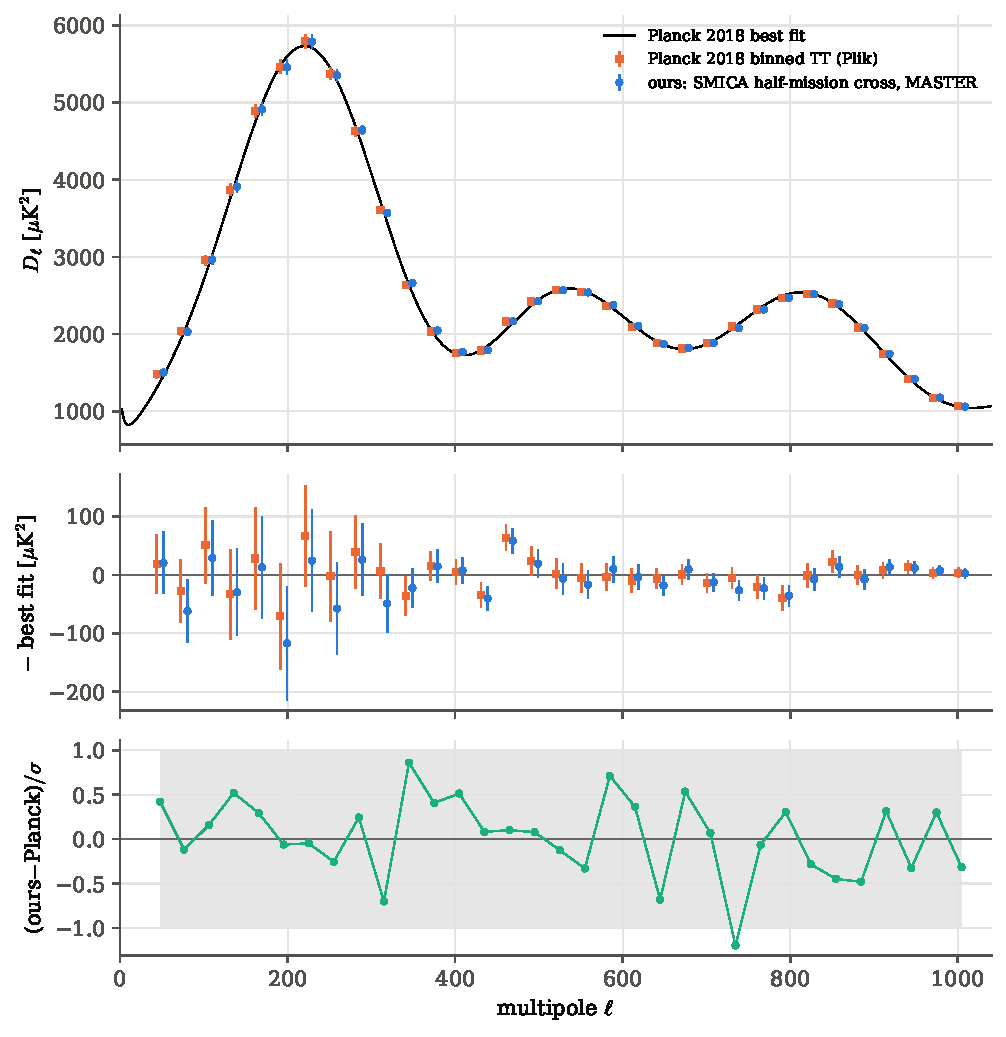
\includegraphics[width=11cm]{figures/ch13/compare.pdf}
\caption{Top: our MASTER bandpowers of the SMICA half-mission cross-spectrum (blue) and \textit{Planck}'s
binned TT spectrum (orange), shifted by $\pm4$ in $\ell$ to be seen side by side, with the best fit (black).
Middle: both minus the best fit; each with its own error bars. Bottom: their difference in units of our
error bar; the grey band is $\pm1$.}
\label{13a:fig:compare}
\end{figure}

\Cref{13a:fig:compare} puts the two spectra on one plot. Over the $\TwelveAP$ bins they differ by
$\TwelveADiffRms\,\mu{\rm K}^2$ in the root mean square, $\TwelveADiffOverSigPl$ of \textit{Planck}'s error bar, and no bin
differs by more than $|\TwelveAWorstSig|$ of ours (at $\ell\approx\TwelveAWorstL$). The error bars themselves are almost equal:
ours are $\TwelveASigOursOverPl$ of \textit{Planck}'s (median over the bins). An overall calibration difference would show up as a
ratio different from one; the inverse-variance weighted mean of our bandpower divided by theirs is
$\TwelveARatioPl$.

\subsection{Why they differ, and by how much they should}
\label{13a:sec:why}

Two measurements of the \emph{same} sky do not scatter around each other like two independent skies. Most of
the error bar of each is cosmic variance, the luck of the particular sky, and the two share it. So the question
``are $\TwelveADiffRms\,\mu{\rm K}^2$ differences reasonable?'' needs the scatter of the \emph{difference} of two
estimators on one sky, and we can measure that with our simulations. Take the main window and the window with
$|b|>30^\circ$, a part of the same sky, and compute both on each simulated sky. Their bandpowers are correlated
with coefficient $\TwelveARhoNested$, and their difference scatters by $\TwelveADiffNestedOverSig$ of the main error
bar. The reason is a simple identity. Nested regions share their sky, so write the smaller-sky estimate as the larger-sky
estimate plus an extra piece, $A_{\rm small}=A_{\rm large}+E$, where $E$ is what the less informative estimate adds, independent of $A_{\rm large}$
(the larger-sky estimate is the more precise one, and that is what makes the extra piece uncorrelated with it). The variance of a sum of
independent pieces is the sum of the variances, $\sigma^2_{\rm small}=\sigma^2_{\rm large}+\Var(E)$, and the difference
$A_{\rm small}-A_{\rm large}=E$ has variance $\sigma^2_{\rm small}-\sigma^2_{\rm large}$. So it scatters by
$\sqrt{(\sigma_{\rm small}/\sigma_{\rm large})^2-1}=\sqrt{\TwelveACutOverMain^2-1}\approx0.77$ of the larger-sky error bar,
close to the measured $\TwelveADiffNestedOverSig$.

\textit{Planck}'s analysis uses a sky that overlaps ours far more than the $|b|>30^\circ$ cut does (its masks keep
$47$--$66\%$ of the sky, almost all of it inside our $\TwelveAFskyMain$), so the expected scatter of
our difference is smaller than $\TwelveADiffNestedOverSig$ of an error bar. We measure $\TwelveADiffOverSigPl$. The rest of
the difference has identifiable causes, each small:
\begin{itemize}[itemsep=2pt]
  \item \emph{Different maps.} SMICA cleans foregrounds by weighting frequencies, Plik by modelling them. Where the
        foreground model and SMICA's weights disagree, the spectra differ; this is largest at high $\ell$, where
        unresolved galaxies add power. Above $\ell=700$ our bandpowers are on average $\TwelveADiffHigh\pm\TwelveADiffHighErr\,\mu{\rm K}^2$
        from \textit{Planck}'s: no sign of excess point-source power in SMICA at these multipoles.
  \item \emph{Different weights on the sky.} Different masks, and inside them different weights per frequency, sample the
        sky's fluctuations differently, which is the part estimated above.
  \item \emph{Different best fits.} Our fiducial is the TT,TE,EE+lowE+lensing best fit, theirs in the file is
        their own; through our windows the two differ by up to $\TwelveABfDiffMax\%$, which matters for the middle panel of
        \cref{13a:fig:compare} but not for the difference of the two measurements.
\end{itemize}

\paragraph{What reproducing it taught us.} A component-separated map, a common mask, our own coupling
matrix and four hundred simulated skies at a sixteenth of the resolution give \textit{Planck}'s temperature spectrum to a
fraction of its error bar and its amplitude to $0.2\%$. What the comparison could not show by itself is how small the
difference \emph{should} be; for that we needed the joint scatter of two estimators on one sky, which only the
simulations provide.
\section{Is anything else in the map? The checks}
\label{13a:sec:checks}

The comparison with \textit{Planck} told us that our spectrum agrees with theirs. It did not tell us that
either spectrum is the spectrum of the CMB alone. Both could share a residual of the Galaxy, both are built
from the same detectors, and a successful comparison between two analyses of one data set is weak evidence
about what is in the data. Recall the three candidate explanations of the map listed in
\cref{13a:sec:question}: a Gaussian isotropic CMB plus noise; residual foregrounds; something the processing
did. The checks are how we put the second and third candidates on trial.

\paragraph{The idea of a null test.} Choose a quantity that the first explanation predicts to be zero on
average, and that the others would push away from zero. Spectra measured through two different windows are
the standard example. If the map outside the mask is a statistically isotropic CMB, the spectrum through the
northern half and the spectrum through the southern half have the same mean; their difference has mean zero.
A residual of the Galaxy that is brighter in one hemisphere, or a stripe left by the scanning, would make it
nonzero. The test then asks the question of every hypothesis test (\cref{4a:sec:null}): if the map were only
CMB and noise, would a difference as large as the one we see, or larger, be something we would reasonably
expect?

\paragraph{Why simulations, and not a formula.} The answer needs the sampling distribution of the difference.
The obvious guess, that the difference of two bandpowers has variance $\sigma_A^2+\sigma_B^2$, is badly wrong
whenever the two windows see the same sky. Take the binary common mask and the apodised window: almost the
same pixels, slightly different weights. The simulations give a scatter of their difference of only
$\TwelveAApoSdOverSig$ of a single bandpower's error, while $\sqrt{\sigma_A^2+\sigma_B^2}$ would be about
$\sqrt2=1.4$ of it, three times too large, and a test built on it could never fail. The difference has the
variance $\sigma_A^2+\sigma_B^2-2\Cov(A,B)$, and the covariance of two estimators on one sky is exactly what our
simulations contain, because each simulated sky is analysed through all five windows. So every test uses the
same recipe:
\begin{enumerate}[itemsep=2pt,leftmargin=1.5em]
  \item the difference vector $\bm\delta$ of the data, over the $\TwelveAP$ bins;
  \item the same difference on each of the $\TwelveANsimUsed$ simulated skies, giving its mean $\bar{\bm\delta}$ and
        covariance $\Cmat_\delta$;
  \item $\chi^2=(\bm\delta-\bar{\bm\delta})\T\Psi_\delta(\bm\delta-\bar{\bm\delta})$, with $\Psi_\delta$ the Hartlap-corrected
        inverse of $\Cmat_\delta$;
  \item the probability to exceed (PTE): the fraction of simulated skies whose $\chi^2$, computed in the same way,
        is at least as large as the data's. For comparison, also the tail of $\chi^2_{33}$ above the data's value.
\end{enumerate}

\begin{figure}[htbp]
\centering
\begin{tikzpicture}
\begin{axis}[width=10cm,height=4.4cm,xmin=0,xmax=80,ymin=0,ymax=0.088,scaled y ticks=false,
  xlabel={$\chi^2$ of a difference vector, $p=33$},ylabel={density},
  yticklabels={},tick label style={font=\footnotesize},label style={font=\small},
  legend style={font=\footnotesize,at={(0.98,0.97)},anchor=north east}]
  \addplot[very thick,formblue,domain=0.5:80,samples=200]
    {exp(15.5*ln(x)-x/2-40.7147)};
  \addlegendentry{distribution under the null}
  \addplot[fill=bdryred!25,draw=none,domain=48:80,samples=60,forget plot]
    {exp(15.5*ln(x)-x/2-40.7147)} \closedcycle;
  \addplot[fill=tangentgreen!25,draw=none,domain=0.5:18,samples=60,forget plot]
    {exp(15.5*ln(x)-x/2-40.7147)} \closedcycle;
  \draw[thick,bdryred] (axis cs:48,0) -- (axis cs:48,0.042);
  \draw[thick,tangentgreen!70!black] (axis cs:18,0) -- (axis cs:18,0.042);
  \node[font=\footnotesize,bdryred,anchor=south,align=center] at (axis cs:56,0.042) {too large:\\ contamination?};
  \node[font=\footnotesize,tangentgreen!50!black,anchor=south,align=center] at (axis cs:12,0.042) {too small:\\ wrong model\\ of scatter?};
\end{axis}
\end{tikzpicture}
\caption{Reading a null test. Under the null hypothesis (CMB and our noise model, nothing else) the $\chi^2$ of a
difference vector of $33$ bandpowers follows the blue curve, which the simulations sample. A value in the right
tail (red) means the difference is larger than chance allows: something in the data is not in the model. A value in
the left tail (green) means it is \emph{smaller} than chance allows: the model of the scatter is wrong, because
contamination can only add to a difference.}
\label{13a:fig:nulllogic}
\end{figure}

\subsection{Four tests, and what each is for}
\label{13a:sec:tests}

\begin{table}[htbp]
\centering\footnotesize
\begin{tabular}{@{}llccc@{}}
\toprule
difference & what would make it nonzero & $\chi^2$ ($p=33$) & PTE (sims) & PTE ($\chi^2_{33}$)\\
\midrule
north $-$ south & anisotropy, a one-sided residual & $\TwelveAHemiChi$ & $\TwelveAHemiPteSims$ & $\TwelveAHemiPteChi$\\
$|b|>30^\circ$ $-$ main & Galactic residuals near the plane & $\TwelveACutChi$ & $\TwelveACutPteSims$ & $\TwelveACutPteChi$\\
binary $-$ apodised & an error in the mode-coupling correction & $\TwelveAApoChi$ & $\TwelveAApoPteSims$ & $\TwelveAApoPteChi$\\
half-mission null & a wrong noise model, sky in the difference & $\TwelveANullChi$ & $\TwelveANullPteSims$ & $\TwelveANullPteChi$\\
\bottomrule
\end{tabular}
\caption{The checks. Each line is a difference that a Gaussian CMB plus our noise model predicts to vanish on
average; the PTE is the fraction of simulated skies with a larger $\chi^2$, and the tail probability of a $\chi^2$
with $33$ degrees of freedom.}
\label{13a:tab:checks}
\end{table}

\begin{figure}[htbp]
\centering
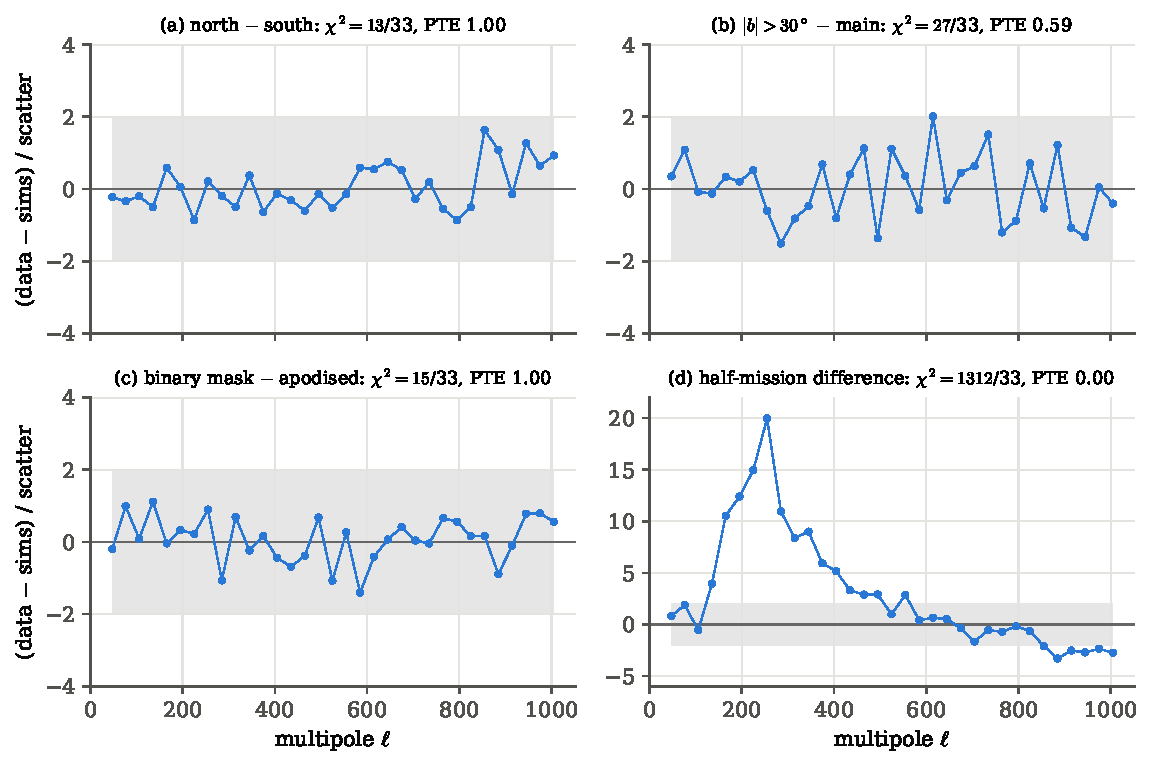
\includegraphics[width=12.4cm]{figures/ch13/checks.pdf}
\caption{The four checks, bin by bin: the data's difference minus the average simulated difference, in units of the
simulated scatter. The grey band is $\pm2$. (a)--(c) compare spectra through different windows; (d) is the spectrum
of the half-mission difference map against the simulated noise.}
\label{13a:fig:checks}
\end{figure}

\paragraph{The Galactic test passes.} The window with $|b|>30^\circ$ removes everything within $30^\circ$ of the plane, where
dust and synchrotron residuals would be strongest. Its spectrum differs from the main one by $\chi^2=\TwelveACutChi$ for
$33$ bins, a PTE of $\TwelveACutPteSims$ (\cref{13a:fig:checks}b). How small a residual could it have seen? The
scatter of this difference is $\TwelveACutSdOverSig$ of a main error bar, so a residual that changed the main
spectrum by a full error bar in several bins would have been detected; one much smaller than that could hide.

\paragraph{The half-mission null fails, and we can say why.} Here the result is unambiguous: $\chi^2=\TwelveANullChi$
for $33$ bins, with single bins $\TwelveANullMaxPull$ standard deviations off (\cref{13a:fig:checks}d). The event: the
spectrum of the half-difference map is up to $\TwelveANullRatioMax$ times the simulated one, at $\ell\approx\TwelveANullRatioL$,
and about $1\%$ \emph{below} it at high $\ell$ (on average $\TwelveANullRatioHigh$ of it above $\ell=600$). What could have
produced it? We take the candidates one at a time.
\begin{enumerate}[itemsep=2pt,leftmargin=1.5em]
  \item \emph{Our noise model has the wrong shape in $\ell$.} It was built as a modulated isotropic field
        \eqref{13a:eq:noise-model}, with a spectrum averaged over 31 multipoles. If the real noise has a different spectrum in
        different parts of the sky, as SMICA's noise does, the product of one map $v$ and one spectrum cannot reproduce it.
        This predicts a mismatch that varies slowly with $\ell$, with either sign.
  \item \emph{Some sky survives in the difference.} If the two halves see the sky with slightly different gains, $1+\epsilon/2$
        and $1-\epsilon/2$ (a calibration difference, or a slightly different effective beam), the difference map contains
        $\epsilon/2$ times the sky, and its spectrum contains $(\epsilon/2)^2$ times the sky's spectrum. This predicts an excess
        that follows the acoustic peaks, largest at the first one.
  \item \emph{The noise of the halves is correlated.} Correlated noise would \emph{cancel} in the difference and lower its
        spectrum, not raise it. It cannot produce an excess.
\end{enumerate}
How well does each explain the data? The excess peaks at $\ell\approx\TwelveANullRatioL$, the first acoustic peak, which is what
the second candidate predicts. Fitting the excess below $\ell=600$ as $(\epsilon/2)^2$ times the fiducial bandpowers plus a constant
gives $\epsilon=\TwelveANullGainEps\%$, and explains $\TwelveANullExcessExplained\%$ of the variance of the excess; the rest, and the
deficit at high $\ell$, is the first candidate. So both are at work: a percent-level difference between the halves' response to
the sky, and a noise model whose shape is good to a few per cent at high $\ell$ and worse at low $\ell$.

The test is this sensitive because the noise is measured with enormous precision: thousands of modes in each bin, and a
simulated scatter of about $2\%$ of the noise power. Does the failure matter for the cross-spectrum? Neither cause biases
it. A gain difference changes the cross-spectrum by the factor $(1+\epsilon/2)(1-\epsilon/2)=1-\epsilon^2/4$, a change of
$\TwelveANullCrossEffect\%$. A noise model wrong by $30\%$ changes only the noise part of the error bars, and the noise is
$\TwelveANullOverSignalMid\%$ of the signal at $\ell\approx500$ and $\TwelveANullOverSignal\%$ at $\ell\approx1000$. The failure is real,
it is understood, and it is harmless for the questions we are asking; a likelihood that used the auto-spectra, where the noise
must be subtracted, could not ignore it. (The identity \eqref{13a:eq:cross-identity} between the full-mission, the cross and the
null spectra holds on the data to $\TwelveAIdentityMax\,\mu{\rm K}^2$ at worst, not exactly, for the same reason: the SMICA full-mission
map is not exactly the average of the two halves.)

\paragraph{Two tests are passed too well.} The hemisphere test gives $\chi^2=\TwelveAHemiChi$ and the apodisation test
$\chi^2=\TwelveAApoChi$, for $33$ bins each. Only $\TwelveAHemiLower$ and $\TwelveAApoLower$ of the $\TwelveANsimUsed$ simulated skies
give smaller values (\cref{13a:tab:checks}, where a PTE of $1.00$ means ``larger than in almost every simulation''). The data's
differences are, bin by bin, $\TwelveAHemiRmsPull$ and $\TwelveAApoRmsPull$ of the simulated scatter in the root mean square,
against about one expected (and $\TwelveACutRmsPull$ for the Galactic test). What could produce two differences this small?
\begin{enumerate}[itemsep=2pt,leftmargin=1.5em]
  \item \emph{Chance.} So few simulated skies fall this low that their count only bounds the chance: a $\chi^2$
        this low happens in at most about $\TwelveALowFracUp$ of skies ($95\%$ upper limit). In the simulations the two
        tests are independent (the correlation of their $\chi^2$ over the simulated skies is $\TwelveALowCorr$), so two of
        four tests this low has a probability below about $\TwelveALowTwoOfFourUp$. Not plausible.
  \item \emph{A residual foreground.} No: contamination adds to a difference, it cannot remove one (\cref{13a:fig:nulllogic}).
  \item \emph{The simulations overestimate the scatter of these differences.} The real map's spectra through different
        windows agree better than Gaussian skies passed through our model of the observation would. Our simulations
        lack two things the real map has been through: SMICA's component separation, and the inpainting that fills the
        holes (the band limit of the degrade spreads the filled values a few arcminutes into the kept pixels at the hole
        edges, exactly where the binary and apodised windows differ).
\end{enumerate}
The third explanation is the likely one, and it limits what the simulations can certify: they describe the scatter of
each window's spectrum well (the best-fit $\chi^2$ of \cref{13a:sec:compare-what} is normal) but overestimate the
scatter of the differences between windows. A low $\chi^2$ cannot hide a contaminant, so the spectrum itself is not
in question. What the full analysis would do is run the null tests on end-to-end simulations processed exactly as the data
were, component separation and inpainting included, which our Gaussian skies are not.

\paragraph{Example: reading a PTE of $1.00$ correctly.} A PTE close to one is not ``a perfect pass''. The PTE is
uniform between $0$ and $1$ when the null hypothesis and its simulated distribution are right (\cref{4a:sec:p-uniform}), so a value
above $0.99$ is as unusual as one below $0.01$. A table of null tests whose PTEs cluster near one is a warning that the
error model is too generous, just as a cluster near zero is a warning of contamination.
\section{Two primordial numbers from the real sky}
\label{13a:sec:fit}

In \cref{9c:sec:planck} the Metropolis sampler of \cref{ch:09} was pointed at a mock \textit{Planck}-like spectrum:
$2\le\ell\le2500$, one $143$\,GHz-like channel, $\fsky=\NineCPlFsky$. With the amplitude and the tilt of the primordial
spectrum free and everything else fixed, it returned errors of $\NineCPlTwoSA$ on $\ln(10^{10}A_s)$ and $\NineCPlTwoSN$
on $n_s$, with a correlation of $\NineCPlTwoRho$; freeing the optical depth $\tau$ inflated the first error ninefold, to
$\NineCPlThreeSA$, because the temperature spectrum above $\ell=30$ measures only the combination $A_se^{-2\tau}$
\eqref{9c:eq:As-tau}. Those were forecasts on a spectrum whose truth we chose. Now the same two parameters, the same
emulator and the same sampler meet our bandpowers of the real sky.

\paragraph{The event, and the hypotheses.} The observed event is our vector of $\TwelveAP$ bandpowers $\widehat{\bm D}$. The
hypotheses are the pairs $\params=(\ln10^{10}A_s,\,n_s)$, with the baryon and dark-matter densities, the angular size of the
sound horizon and $\tau$ held at the \textit{Planck} best fit. For each pair the question is: had nature chosen these values,
how plausible would the fluctuation be that turns the predicted bandpowers into the ones we measured? That is the
likelihood of \eqref{13a:eq:like}, and Bayes' theorem with a flat prior over $2.8<\ln10^{10}A_s<3.3$, $0.85<n_s<1.10$ turns it into
a posterior.

\subsection{The model, the likelihood and the sampler}
\label{13a:sec:fit-setup}

\emph{The model.} The predicted bandpowers are $\bm t(\params)=\mathcal F\,\bm C(\params)$: the theory spectrum passed through the
bandpower windows \eqref{13a:eq:bpw}. The spectrum $\Cell(\params)$ comes from the emulator of \cref{9c:sec:emu}, a second-order
Taylor expansion of $\ln\Cell$ about the fiducial \eqref{9c:eq:emu}, which reproduces CAMB to far better than our error bars
over this range (\cref{9c:sec:emu-check}). A CAMB call takes seconds; the emulator takes microseconds, so a chain of tens
of thousands of steps costs seconds.

\emph{The likelihood.} Gaussian in the bandpowers, \eqref{13a:eq:like}, with the simulated covariance and the Hartlap factor.
The covariance is held fixed at the fiducial model, as \textit{Planck} does; over the narrow range of parameters the data
allow, the change of the covariance with the parameters is negligible \cite{HamimecheLewis2008}.

\emph{The sampler.} Random-walk Metropolis (\cref{9b:sec:biased}), \texttt{code/ch09/lib\_mcmc.py}, with a Gaussian proposal
whose shape is the inverse Fisher matrix $\Fish^{-1}$ and whose scale is $2.38/\sqrt d$ for $d=2$ parameters, the rule of
\cref{9b:sec:stepsize}. Four chains of $20\,000$ steps start from points scattered over three Fisher widths around the
fiducial; the first $20\%$ of each is discarded as burn-in (\cref{9b:sec:burnin}).

\paragraph{Example: the Fisher matrix as a first answer.} For a model that is linear in the parameters near the peak, the
posterior is Gaussian with covariance $\Fish^{-1}$, where $\Fish=J\T\Psi J$ and $J_{bi}=\partial t_b/\partial\theta_i$
(\cref{ch:10}). We compute $J$ by central differences of the emulator. The Fisher errors are $\TwelveAFisherSA$ on
$\ln10^{10}A_s$ and $\TwelveAFisherSN$ on $n_s$. The chains give $\TwelveAFitSA$ and $\TwelveAFitSN$. Agreement to within a few per cent says the posterior is Gaussian to that precision: over a range of $\pm3\sigma$ the bandpowers depend on the two parameters
almost linearly.

\pyfile[firstline=49,lastline=56]{code/ch13/07_fit.py}{The log-posterior: a flat prior and the Gaussian bandpower likelihood}

\noindent The function returned by \pyname{make_logpost} is all the sampler sees. Outside the prior box it returns $-\infty$, so
every proposal there is rejected. Inside, it computes the residual between the bandpowers and the emulated theory through the
windows, and returns $-\tfrac12\chi^2$; the normalisation of the posterior never appears, because Metropolis only uses ratios
(\cref{9b:sec:ratios}).

\subsection{What the real sky says}
\label{13a:sec:fit-results}

The chains are healthy: acceptance $\TwelveAFitAcc$, integrated autocorrelation time about $\TwelveAFitTau$ steps
(\cref{9b:sec:tau}), so the $64\,000$ kept samples are worth several thousand independent ones, and the split $\hat R$ of the
four chains is $\TwelveAFitRhat$ (\cref{9b:sec:rhat}). The posterior means and standard deviations are
\begin{equation}
  \ln(10^{10}A_s)=\TwelveAFitA\pm\TwelveAFitSA,\qquad n_s=\TwelveAFitN\pm\TwelveAFitSN,\qquad\rho=\TwelveAFitRho ,
  \label{13a:eq:fit}
\end{equation}
and at the maximum of the likelihood $\chi^2=\TwelveAChiMl$ for $\TwelveAP-2=31$ degrees of freedom (a tail probability of
$\TwelveAPteMl$): two parameters describe the $\TwelveAP$ bandpowers as well as they should. With $\tau=\TwelveATau$ fixed, the
quantity the temperature spectrum actually measures is $10^9A_se^{-2\tau}=\TwelveAFitAsE\pm\TwelveAFitSAsE$.

To separate what comes from \emph{our} bandpowers from what comes from the multipole range, we run the same fit, same emulator,
same sampler, on \textit{Planck}'s published bandpowers, with their quoted errors as a diagonal covariance (the file gives no
correlations): first over our range $30\le\ell\le1019$, then over $30\le\ell\le\TwelveAPlFullLmax$, as far as our emulator goes.

\begin{table}[htbp]
\centering\small
\begin{tabular}{@{}lccc@{}}
\toprule
data, multipoles, free parameters & $\ln(10^{10}A_s)$ & $n_s$ & $\rho$\\
\midrule
ours (SMICA), $30$--$1019$, 2 free & $\TwelveAFitA\pm\TwelveAFitSA$ & $\TwelveAFitN\pm\TwelveAFitSN$ & $\TwelveAFitRho$\\
\textit{Planck} bandpowers, $30$--$1019$, 2 free & $\TwelveAPlSameA\pm\TwelveAPlSameSA$ & $\TwelveAPlSameN\pm\TwelveAPlSameSN$ & $\TwelveAPlSameRho$\\
\textit{Planck} bandpowers, $30$--$\TwelveAPlFullLmax$, 2 free & $\TwelveAPlFullA\pm\TwelveAPlFullSA$ & $\TwelveAPlFullN\pm\TwelveAPlFullSN$ & $\TwelveAPlFullRho$\\
mock spectrum of \cref{9c:sec:planck}, $2$--$2500$, 2 free & $\pm\NineCPlTwoSA$ & $\pm\NineCPlTwoSN$ & $\NineCPlTwoRho$\\
\textit{Planck} 2018 VI, TT+lowE, 6 free & $\TwelveAPubA\pm\TwelveAPubSA$ & $\TwelveAPubN\pm\TwelveAPubSN$ & \\
\bottomrule
\end{tabular}
\caption{The amplitude and tilt from our bandpowers, from \textit{Planck}'s bandpowers through the same fit, from the
forecast of \cref{9c:sec:planck}, and as published with all six parameters free \cite{Planck2018VI}.}
\label{13a:tab:fit}
\end{table}

\begin{figure}[htbp]
\centering
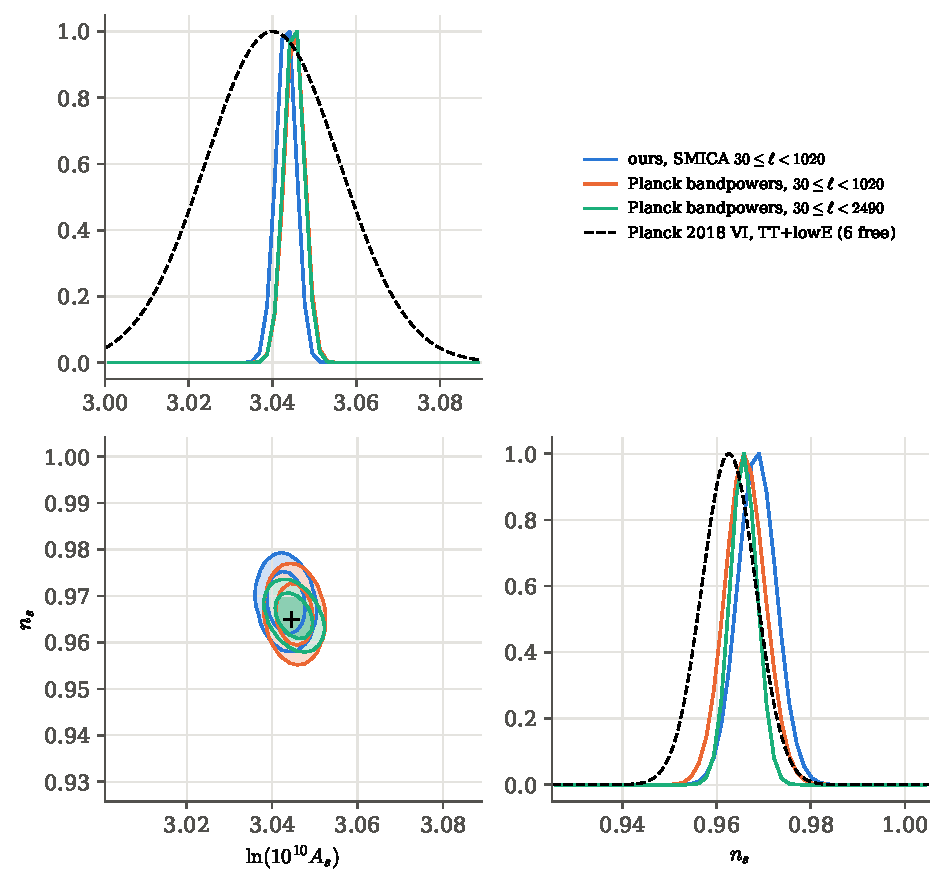
\includegraphics[width=10cm]{figures/ch13/fit.pdf}
\caption{Posteriors of $\ln(10^{10}A_s)$ and $n_s$ with the other four parameters fixed: from our SMICA bandpowers (blue),
from \textit{Planck}'s bandpowers over the same multipoles (orange) and over $30\le\ell\le\TwelveAPlFullLmax$ (green). Contours enclose
$68\%$ and $95\%$. The black dashed curves are the published one-dimensional results with all six parameters free; the cross
is the fiducial.}
\label{13a:fig:fit}
\end{figure}

\subsection{Reading the comparison with \textit{Planck} 2018 VI}
\label{13a:sec:fit-planck}

\paragraph{Their question and setup.} \textit{Planck} 2018 VI asked which $\Lambda$CDM parameters the CMB spectra prefer. Its
``TT+lowE'' result combines the high-$\ell$ temperature likelihood of \eqref{13a:eq:plik}, a low-$\ell$ temperature likelihood for
$2\le\ell<30$, and the large-scale $E$-mode polarisation, which measures $\tau$. All six parameters are free, together with
nuisance parameters for the foregrounds and the calibration \cite{Planck2018VI}. Its key equation is the same Gaussian likelihood
we derived in \cref{13a:sec:gauss-like}, multiplied by the low-$\ell$ terms.

\paragraph{Side by side, and why the numbers differ.} \Cref{13a:fig:fit} and \cref{13a:tab:fit} show three differences, each with
a cause we can name.
\begin{enumerate}[itemsep=3pt,leftmargin=1.5em]
  \item \emph{Our error on the amplitude is nine times smaller.} Above $\ell=30$ the temperature spectrum depends on $A_s$ and $\tau$
        only through $A_se^{-2\tau}$, so $\ln(10^{10}A_s)=\ln(10^{10}A_se^{-2\tau})+2\tau$ and, the two terms being nearly
        independent, $\sigma^2(\ln10^{10}A_s)\approx\sigma^2(\ln10^{10}A_se^{-2\tau})+4\sigma_\tau^2$ \eqref{9c:eq:As-tau}. We fixed
        $\tau$, so the second term is zero and we quote the error of the first, $\TwelveAFitSA$. \textit{Planck} measures
        $\sigma_\tau=0.008$ from polarisation, and $2\times0.008=0.016$ is its whole error on $\ln(10^{10}A_s)$. The well-measured
        combination agrees: $10^9A_se^{-2\tau}=\TwelveAFitAsE\pm\TwelveAFitSAsE$ for us, $\TwelveAPubAsE\pm\TwelveAPubSAsE$ published.
  \item \emph{Our error on $n_s$ is smaller than theirs although we use two fifths of the multipoles.} With six parameters free, a change of
        the tilt can be partly undone by a change of the baryon density, which also tilts the relative heights of the peaks; fixing the
        other parameters removes that escape route. Freeing them costs a factor of about two in \cref{9c:sec:planck} ($\NineCPlTwoSN$ to
        $\NineCPlSixSN$), the same factor that separates our full-range fit of \textit{Planck}'s bandpowers ($\TwelveAPlFullSN$) from the
        published $\TwelveAPubSN$.
  \item \emph{The multipole range matters for the tilt.} On \textit{Planck}'s bandpowers, going from $\ell\le1019$ to $\ell\le\TwelveAPlFullLmax$
        shrinks the error on $n_s$ from $\TwelveAPlSameSN$ to $\TwelveAPlFullSN$ and strengthens the anticorrelation with the amplitude from
        $\TwelveAPlSameRho$ to $\TwelveAPlFullRho$. A tilt is a lever, and the damping tail lengthens the arm; on a longer arm, raising the amplitude
        and lowering the tilt compensate each other over more of the range, hence the stronger correlation. The full-range numbers reproduce
        the forecast of \cref{9c:sec:planck} ($\NineCPlTwoSA$, $\NineCPlTwoSN$, $\NineCPlTwoRho$): that forecast described the real data correctly.
\end{enumerate}
The central values agree within the errors. Our $n_s=\TwelveAFitN$ sits one standard deviation above the fiducial $\TwelveAFidNs$, and
$0.6\sigma$ above the fit to \textit{Planck}'s bandpowers over the same range; the bin-by-bin differences of \cref{13a:sec:side}, a few tenths of
an error bar each, are enough to move a two-parameter fit that much.

\subsection{Do the low and the high multipoles agree?}
\label{13a:sec:split}

A fit to a range of multipoles averages over it. If the low and the high multipoles wanted different parameters, the average would
hide it, and \textit{Planck} took this question seriously: in their temperature data some parameters differ by more than $2\sigma$
between $\ell<800$ and $\ell>800$, which they judge, after accounting for correlations, not to be especially unusual
\cite[p.~32]{Planck2018VI}. We ask the same of our data, splitting at $\ell=\TwelveASplit$ so that both halves have similar
constraining power.

\paragraph{The test statistic.} Fit $(\ln10^{10}A_s,n_s)$ separately to the bins below and above the split, and form the shift
$\bm\Delta=\hat\params_{\rm low}-\hat\params_{\rm high}$. If both halves measure the same sky with the same model, $\bm\Delta$ has mean zero.
Its covariance is not the sum of the two fits' covariances, since the two halves share the mask and are weakly correlated, so we take it
from the simulations: the same two fits on each simulated sky give $\TwelveANsimUsed$ shifts and their covariance $\Cmat_\Delta$. Then
$\chi^2=\bm\Delta\T\Cmat_\Delta^{-1}\bm\Delta$ has two degrees of freedom.

\paragraph{The result.} The low multipoles prefer $(\TwelveALoA,\,\TwelveALoN)$ and the high ones $(\TwelveAHiA,\,\TwelveAHiN)$. The shift is
$\Delta\ln10^{10}A_s=\TwelveADeltaA\pm\TwelveADeltaSA$ and $\Delta n_s=\TwelveADeltaN\pm\TwelveADeltaSN$, and $\chi^2=\TwelveASplitChi$. A
fraction $\TwelveASplitPte$ of the simulated skies gives a larger one, the same as the $\chi^2_2$ tail ($\TwelveASplitPteChi$;
\cref{13a:fig:split}). The amplitude shift alone is a $2\sigma$ effect, but one of two correlated numbers at $2\sigma$ is what the
two-dimensional test is for: it is a one-in-nine event, and the two halves agree.

\begin{figure}[htbp]
\centering
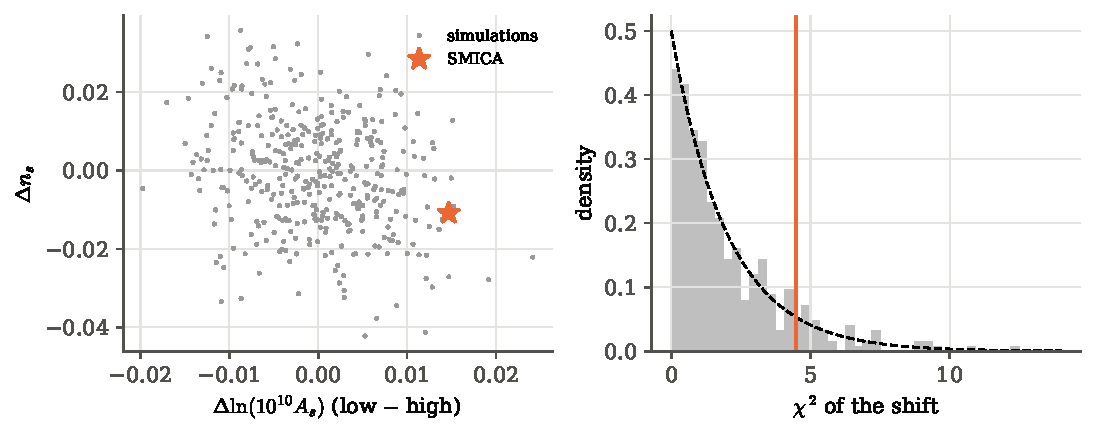
\includegraphics[width=11.4cm]{figures/ch13/split.pdf}
\caption{Low against high multipoles. Left: the shift between the parameters fitted to $\ell<\TwelveASplit$ and to $\ell>\TwelveASplit$ on each
simulated sky (grey) and on the SMICA bandpowers (star). Right: the $\chi^2$ of the shift over the simulations (histogram), the $\chi^2_2$
density (dashed), and the data (vertical line).}
\label{13a:fig:split}
\end{figure}

\begin{pitfall}[A fixed parameter is a prior of zero width]
Holding four parameters at their best-fit values is the same as giving them delta-function priors. The errors in \eqref{13a:eq:fit}
are therefore \emph{conditional} errors, smaller than the marginal ones of a six-parameter fit, and the central values inherit any
error in the fixed values. Our $\pm\TwelveAFitSA$ on $\ln(10^{10}A_s)$ is not a better measurement than \textit{Planck}'s $\pm0.016$; it is the
answer to a narrower question.
\end{pitfall}
\section{The full analysis, and what the laptop version gives up}
\label{13a:sec:research}

Everything above ran on four processor cores: the preparation of the maps in under a minute, each simulated sky in
$\TwelveASecPerSky$\,s, the four hundred of them in about ten minutes, the fits in seconds. \textit{Planck}'s analysis of the
same sky used supercomputers for years. Each place where we took a shorter road costs something, and an honest result says
what. \Cref{13a:tab:nerf} lists the reductions, and the paragraphs after it put a size on the ones that matter.

\begin{table}[htbp]
\centering\small
\begin{tabularx}{\linewidth}{@{}>{\raggedright}p{2.3cm}>{\raggedright}X>{\raggedright}X>{\raggedright\arraybackslash}X@{}}
\toprule
step & full analysis (\textit{Planck} 2018) & ours & what the reduction costs\\
\midrule
maps & $100$, $143$, $217$\,GHz half-missions, $N_{\rm side}=2048$ & SMICA half-missions degraded to $N_{\rm side}=512$ & multipoles above $1019$; foreground uncertainty not propagated\\
multipoles & $30$--$2508$ (plus a separate $2$--$29$ likelihood) & $30$--$1019$ & error on $n_s$ $\TwelveAPlSameSN$ instead of $\TwelveAPlFullSN$ on the same bandpowers\\
masks & per frequency, $47$--$66\%$ of the sky & one common mask, $\TwelveAFskyMain$ & more exposure to residuals near the plane\\
foregrounds & modelled, amplitudes marginalised & cleaned by SMICA, then ignored & residuals at high $\ell$ unmodelled\\
beams & beam matrices per cross-spectrum, with leakage & one effective beam & a beam error would tilt $n_s$\\
covariance & analytic, validated on FFP10 end-to-end simulations & $\TwelveANsimUsed$ Gaussian skies, noise model from the data & errors uncertain by $\TwelveAMcErrSig\%$; null and window-difference tests not validated\\
parameters & six, plus nuisance parameters, $\tau$ from polarisation & two, four fixed & conditional, not marginal, errors\\
\bottomrule
\end{tabularx}
\caption{The full analysis and the laptop analysis, step by step.}
\label{13a:tab:nerf}
\end{table}

\paragraph{The multipole range.} The largest single cost. Fitting \textit{Planck}'s own bandpowers with our two-parameter model, the
error on $n_s$ is $\TwelveAPlSameSN$ over our range and $\TwelveAPlFullSN$ over theirs (\cref{13a:sec:fit-planck}): the damping tail is
worth a factor $1.6$ on the tilt. Going to $N_{\rm side}=1024$, whose degraded maps already exist in \texttt{data/planck/}, would reach
$\ell\approx2000$ at eight times the cost per transform.

\paragraph{The simulations.} \textit{Planck}'s FFP10 simulations follow the photons through the instrument: time-ordered data
of every detector, the map-maker, and the component separation. Ours start at the map and assume a Gaussian sky and a modulated
Gaussian noise. For the error bars of the spectrum itself the difference is small, because below $\ell\approx1000$ the error is cosmic
variance, which a Gaussian sky gets right; our errors agree with \textit{Planck}'s to within a few per cent
($\TwelveASigOursOverPl$ of theirs, \cref{13a:sec:side}). For the checks it is not small: the half-mission null test fails
because our noise model is too simple, and the window-difference tests come out too good, most likely because the real map has
been through processing that our skies have not (\cref{13a:sec:checks}).

\paragraph{The number of simulations.} With $n=\TwelveANsimUsed$ skies and $p=\TwelveAP$ bins, the Hartlap factor is $\TwelveAHartlap$ and the
error bars are known to $\TwelveAMcErrSig\%$. Doubling $n$ would reduce that to $2.5\%$ at twice the cost; the gain matters for PTEs near the
edges of the distribution, where $1/n$ sets the resolution, as in the two window-difference tests, which only $\TwelveAHemiLower$ and
$\TwelveAApoLower$ of the $\TwelveANsimUsed$ simulated skies beat: too few to say how rare they are, only that they are rare.

\begin{inpractice}[Verification and research in one pipeline]
Two different jobs were done by the same simulations. The bias test of \cref{13a:sec:cov} \emph{verified} a known result: MASTER's mean is
the theory through the bandpower windows, a statement derived in \cref{8b:sec:master}, and the simulations confirmed it to
$1/\sqrt{\TwelveANsimUsed}$ of an error bar. Everything else was \emph{research}: the covariance of masked, noisy, beamed bandpowers, the
scatter of the difference between two windows on one sky, the distribution of a parameter shift between low and high
multipoles. None of these has a formula we trust at the precision needed, and each was read off the simulations directly. Research
codes package the same steps: NaMaster computes the coupling matrix, the binned inverse and the bandpower windows for spin-0 and
spin-2 fields on any mask \cite{Alonso2019}, and \textit{Planck}'s likelihood code evaluates \eqref{13a:eq:plik} with its analytic
covariance. What no library supplies is the model of the observation, which here was ours to build and ours to test.
\end{inpractice}

\paragraph{Every arrow of the pipeline, on real data.} Each arrow of
physical model $\to$ field $\to$ what matters $\to$ summary $\to$ its sampling distribution $\to$ inference was crossed on real data.
The physical model was $\Lambda$CDM with two free numbers. The field was the SMICA map. What mattered was the two-point statistics
of a Gaussian field, so the summary was the binned power spectrum. Its sampling distribution came from four hundred skies observed
like the real one. The inference was a posterior for $A_s$ and $n_s$, and a set of tests that the data passed, failed, or passed
suspiciously well. The same map returns in \cref{13b:sec:question}, where the summary changes from the spectrum to the shapes of
the hot and cold regions, and with it the information it can see.

\begin{recap}
\begin{itemize}[itemsep=2pt]
  \item A map is changed in resolution in harmonic space: multiply the $\alm$ by the ratio of pixel windows and truncate at
        $3N_{\rm side}-1$, after filling the masked holes so that the band limit cannot spread their residuals.
  \item The common mask has a few large holes and thousands of small ones; they are tapered differently ($0.5^\circ$ and $2^\circ$) because a
        wide taper around thousands of holes would cost most of the sky.
  \item The cross-spectrum of the half-mission maps has no noise bias; their half-difference is a null map of the noise.
  \item \textit{Planck}'s bins weight $\Cell$ by $\ell(\ell+1)$ and quote $D_b$ at $\ell^{\rm eff}$; a bandpower is not $D_\ell$ at $\ell^{\rm eff}$, and theory
        must go through the same binning and the bandpower windows.
  \item On the real sky the naive correction is off by $\TwelveANaiveMaxDev\%$ in the troughs; MASTER with our coupling matrix agrees with
        \textit{Planck}'s bandpowers to $\TwelveAMasterMaxDev\%$ at worst.
  \item Four hundred Gaussian skies observed like the real one give the covariance, an unbiasedness test, and the scatter of every
        difference used by the checks.
  \item The best fit describes our bandpowers ($\chi^2=\TwelveAChiBf$ for $33$), the amplitude agrees to $0.2\%$, and our spectrum differs from
        \textit{Planck}'s by $\TwelveADiffOverSigPl$ of an error bar.
  \item Null tests: the Galactic test passes; the half-mission null fails because of a percent-level gain difference between the halves
        and an approximate noise model, neither of which affects the cross-spectrum; two window-difference tests are passed too well,
        a sign that our simulations overestimate the scatter of differences.
  \item With four parameters fixed, $\ln(10^{10}A_s)=\TwelveAFitA\pm\TwelveAFitSA$ and $n_s=\TwelveAFitN\pm\TwelveAFitSN$; the comparison with
        \textit{Planck}'s six-parameter result is explained by $\tau$, by the fixed parameters and by the multipole range.
\end{itemize}
\end{recap}
\providecommand{\PlNside}{}\renewcommand{\PlNside}{256}
\providecommand{\PlFwhm}{}\renewcommand{\PlFwhm}{40}
\providecommand{\PlNsim}{}\renewcommand{\PlNsim}{300}
\providecommand{\PlLmax}{}\renewcommand{\PlLmax}{767}
\providecommand{\PlRatioTh}{}\renewcommand{\PlRatioTh}{108.4}
\providecommand{\PlRatioMC}{}\renewcommand{\PlRatioMC}{108.1}
\providecommand{\PlRatioSd}{}\renewcommand{\PlRatioSd}{2.9}
\providecommand{\PlThetaC}{}\renewcommand{\PlThetaC}{31.7}
\providecommand{\PlPixArcmin}{}\renewcommand{\PlPixArcmin}{13.7}
\providecommand{\PlVonePeakTh}{}\renewcommand{\PlVonePeakTh}{0.0884}
\providecommand{\PlVoneTh}{}\renewcommand{\PlVoneTh}{0.0852}
\providecommand{\PlVoneMC}{}\renewcommand{\PlVoneMC}{0.0851}
\providecommand{\PlVoneSd}{}\renewcommand{\PlVoneSd}{8.000\times10^{-4}}
\providecommand{\PlVoneRead}{}\renewcommand{\PlVoneRead}{0.081}
\providecommand{\PlVtwoTh}{}\renewcommand{\PlVtwoTh}{0.0186}
\providecommand{\PlVtwoMC}{}\renewcommand{\PlVtwoMC}{0.0173}
\providecommand{\PlVtwoSd}{}\renewcommand{\PlVtwoSd}{4.000\times10^{-4}}
\providecommand{\PlVtwoRead}{}\renewcommand{\PlVtwoRead}{0.021}
\providecommand{\PlVtwoTwoFiveSix}{}\renewcommand{\PlVtwoTwoFiveSix}{0.0174}
\providecommand{\PlVtwoFiveOneTwo}{}\renewcommand{\PlVtwoFiveOneTwo}{0.0183}
\providecommand{\PlPixDef}{}\renewcommand{\PlPixDef}{4.8}
\providecommand{\PlChiMean}{}\renewcommand{\PlChiMean}{1.01}
\providecommand{\PlChiMed}{}\renewcommand{\PlChiMed}{0.97}
\providecommand{\PlNdof}{}\renewcommand{\PlNdof}{36}
\providecommand{\PlHartlap}{}\renewcommand{\PlHartlap}{0.876}
\providecommand{\PlChiZero}{}\renewcommand{\PlChiZero}{-172}
\providecommand{\PlChiZeroSe}{}\renewcommand{\PlChiZeroSe}{6}
\providecommand{\PlChiSlope}{}\renewcommand{\PlChiSlope}{4688}
\providecommand{\PlShift}{}\renewcommand{\PlShift}{0.037}
\providecommand{\BfskyFull}{}\renewcommand{\BfskyFull}{77.9}
\providecommand{\BfskySixFour}{}\renewcommand{\BfskySixFour}{71.3}
\providecommand{\BfskyOneTwoEight}{}\renewcommand{\BfskyOneTwoEight}{73.6}
\providecommand{\BfskyTwoFiveSix}{}\renewcommand{\BfskyTwoFiveSix}{74.7}
\providecommand{\BfskyFiveOneTwo}{}\renewcommand{\BfskyFiveOneTwo}{75.5}
\providecommand{\BpowLow}{}\renewcommand{\BpowLow}{0.71}
\providecommand{\BpowMid}{}\renewcommand{\BpowMid}{1.005}
\providecommand{\BpowHigh}{}\renewcommand{\BpowHigh}{1.088}
\providecommand{\BpowHighNoNoise}{}\renewcommand{\BpowHighNoNoise}{1.06}
\providecommand{\BnoiseRatioFive}{}\renewcommand{\BnoiseRatioFive}{0.002}
\providecommand{\BnoiseRatioThousand}{}\renewcommand{\BnoiseRatioThousand}{0.019}
\providecommand{\BnoiseRatioFifteen}{}\renewcommand{\BnoiseRatioFifteen}{0.144}
\providecommand{\BnoiseUkArcmin}{}\renewcommand{\BnoiseUkArcmin}{32}
\providecommand{\BnoiseVarSixFour}{}\renewcommand{\BnoiseVarSixFour}{0.01}
\providecommand{\BnoiseGradSixFour}{}\renewcommand{\BnoiseGradSixFour}{0.03}
\providecommand{\BnoiseVarOneTwoEight}{}\renewcommand{\BnoiseVarOneTwoEight}{0.02}
\providecommand{\BnoiseGradOneTwoEight}{}\renewcommand{\BnoiseGradOneTwoEight}{0.02}
\providecommand{\BnoiseVarTwoFiveSix}{}\renewcommand{\BnoiseVarTwoFiveSix}{0.02}
\providecommand{\BnoiseGradTwoFiveSix}{}\renewcommand{\BnoiseGradTwoFiveSix}{0.03}
\providecommand{\BnoiseVarFiveOneTwo}{}\renewcommand{\BnoiseVarFiveOneTwo}{0.03}
\providecommand{\BnoiseGradFiveOneTwo}{}\renewcommand{\BnoiseGradFiveOneTwo}{0.08}
\providecommand{\MfNSixFour}{}\renewcommand{\MfNSixFour}{1000}
\providecommand{\MfHartSixFour}{}\renewcommand{\MfHartSixFour}{0.963}
\providecommand{\MfChiSixFour}{}\renewcommand{\MfChiSixFour}{23.3}
\providecommand{\MfChiNSixFour}{}\renewcommand{\MfChiNSixFour}{0.65}
\providecommand{\MfPSixFour}{}\renewcommand{\MfPSixFour}{91.7}
\providecommand{\MfPerrSixFour}{}\renewcommand{\MfPerrSixFour}{0.9}
\providecommand{\MfPchiSixFour}{}\renewcommand{\MfPchiSixFour}{94.9}
\providecommand{\MfSimMeanSixFour}{}\renewcommand{\MfSimMeanSixFour}{1}
\providecommand{\MfMaxDevSixFour}{}\renewcommand{\MfMaxDevSixFour}{2.2}
\providecommand{\MfPlanckPSixFour}{}\renewcommand{\MfPlanckPSixFour}{90}
\providecommand{\SzeroDataSixFour}{}\renewcommand{\SzeroDataSixFour}{46.7}
\providecommand{\SzeroSimSixFour}{}\renewcommand{\SzeroSimSixFour}{52.7}
\providecommand{\SzeroSdSixFour}{}\renewcommand{\SzeroSdSixFour}{3.4}
\providecommand{\SzeroRankSixFour}{}\renewcommand{\SzeroRankSixFour}{1.6}
\providecommand{\RatioDataSixFour}{}\renewcommand{\RatioDataSixFour}{27}
\providecommand{\RatioSimSixFour}{}\renewcommand{\RatioSimSixFour}{24.3}
\providecommand{\RatioSdSixFour}{}\renewcommand{\RatioSdSixFour}{1.5}
\providecommand{\MfPAreaSixFour}{}\renewcommand{\MfPAreaSixFour}{92.7}
\providecommand{\MfPLengthSixFour}{}\renewcommand{\MfPLengthSixFour}{64.2}
\providecommand{\MfPGenusSixFour}{}\renewcommand{\MfPGenusSixFour}{78.2}
\providecommand{\MfNOneTwoEight}{}\renewcommand{\MfNOneTwoEight}{1000}
\providecommand{\MfHartOneTwoEight}{}\renewcommand{\MfHartOneTwoEight}{0.963}
\providecommand{\MfChiOneTwoEight}{}\renewcommand{\MfChiOneTwoEight}{32.6}
\providecommand{\MfChiNOneTwoEight}{}\renewcommand{\MfChiNOneTwoEight}{0.91}
\providecommand{\MfPOneTwoEight}{}\renewcommand{\MfPOneTwoEight}{60.3}
\providecommand{\MfPerrOneTwoEight}{}\renewcommand{\MfPerrOneTwoEight}{1.5}
\providecommand{\MfPchiOneTwoEight}{}\renewcommand{\MfPchiOneTwoEight}{63.1}
\providecommand{\MfSimMeanOneTwoEight}{}\renewcommand{\MfSimMeanOneTwoEight}{1}
\providecommand{\MfMaxDevOneTwoEight}{}\renewcommand{\MfMaxDevOneTwoEight}{1.8}
\providecommand{\MfPlanckPOneTwoEight}{}\renewcommand{\MfPlanckPOneTwoEight}{85.4}
\providecommand{\SzeroDataOneTwoEight}{}\renewcommand{\SzeroDataOneTwoEight}{58.7}
\providecommand{\SzeroSimOneTwoEight}{}\renewcommand{\SzeroSimOneTwoEight}{63.4}
\providecommand{\SzeroSdOneTwoEight}{}\renewcommand{\SzeroSdOneTwoEight}{2.7}
\providecommand{\SzeroRankOneTwoEight}{}\renewcommand{\SzeroRankOneTwoEight}{1.6}
\providecommand{\RatioDataOneTwoEight}{}\renewcommand{\RatioDataOneTwoEight}{58.6}
\providecommand{\RatioSimOneTwoEight}{}\renewcommand{\RatioSimOneTwoEight}{54.4}
\providecommand{\RatioSdOneTwoEight}{}\renewcommand{\RatioSdOneTwoEight}{2.3}
\providecommand{\MfPAreaOneTwoEight}{}\renewcommand{\MfPAreaOneTwoEight}{33.6}
\providecommand{\MfPLengthOneTwoEight}{}\renewcommand{\MfPLengthOneTwoEight}{79.8}
\providecommand{\MfPGenusOneTwoEight}{}\renewcommand{\MfPGenusOneTwoEight}{79.6}
\providecommand{\MfNTwoFiveSix}{}\renewcommand{\MfNTwoFiveSix}{500}
\providecommand{\MfHartTwoFiveSix}{}\renewcommand{\MfHartTwoFiveSix}{0.926}
\providecommand{\MfChiTwoFiveSix}{}\renewcommand{\MfChiTwoFiveSix}{34.6}
\providecommand{\MfChiNTwoFiveSix}{}\renewcommand{\MfChiNTwoFiveSix}{0.96}
\providecommand{\MfPTwoFiveSix}{}\renewcommand{\MfPTwoFiveSix}{50}
\providecommand{\MfPerrTwoFiveSix}{}\renewcommand{\MfPerrTwoFiveSix}{2.2}
\providecommand{\MfPchiTwoFiveSix}{}\renewcommand{\MfPchiTwoFiveSix}{53.5}
\providecommand{\MfSimMeanTwoFiveSix}{}\renewcommand{\MfSimMeanTwoFiveSix}{1}
\providecommand{\MfMaxDevTwoFiveSix}{}\renewcommand{\MfMaxDevTwoFiveSix}{1.9}
\providecommand{\MfPlanckPTwoFiveSix}{}\renewcommand{\MfPlanckPTwoFiveSix}{93.9}
\providecommand{\SzeroDataTwoFiveSix}{}\renewcommand{\SzeroDataTwoFiveSix}{75.6}
\providecommand{\SzeroSimTwoFiveSix}{}\renewcommand{\SzeroSimTwoFiveSix}{79.5}
\providecommand{\SzeroSdTwoFiveSix}{}\renewcommand{\SzeroSdTwoFiveSix}{2.3}
\providecommand{\SzeroRankTwoFiveSix}{}\renewcommand{\SzeroRankTwoFiveSix}{2}
\providecommand{\RatioDataTwoFiveSix}{}\renewcommand{\RatioDataTwoFiveSix}{114.1}
\providecommand{\RatioSimTwoFiveSix}{}\renewcommand{\RatioSimTwoFiveSix}{108.7}
\providecommand{\RatioSdTwoFiveSix}{}\renewcommand{\RatioSdTwoFiveSix}{3}
\providecommand{\MfPAreaTwoFiveSix}{}\renewcommand{\MfPAreaTwoFiveSix}{32.4}
\providecommand{\MfPLengthTwoFiveSix}{}\renewcommand{\MfPLengthTwoFiveSix}{59.4}
\providecommand{\MfPGenusTwoFiveSix}{}\renewcommand{\MfPGenusTwoFiveSix}{30}
\providecommand{\MfNFiveOneTwo}{}\renewcommand{\MfNFiveOneTwo}{300}
\providecommand{\MfHartFiveOneTwo}{}\renewcommand{\MfHartFiveOneTwo}{0.876}
\providecommand{\MfChiFiveOneTwo}{}\renewcommand{\MfChiFiveOneTwo}{42.4}
\providecommand{\MfChiNFiveOneTwo}{}\renewcommand{\MfChiNFiveOneTwo}{1.18}
\providecommand{\MfPFiveOneTwo}{}\renewcommand{\MfPFiveOneTwo}{23}
\providecommand{\MfPerrFiveOneTwo}{}\renewcommand{\MfPerrFiveOneTwo}{2.4}
\providecommand{\MfPchiFiveOneTwo}{}\renewcommand{\MfPchiFiveOneTwo}{21.5}
\providecommand{\MfSimMeanFiveOneTwo}{}\renewcommand{\MfSimMeanFiveOneTwo}{1}
\providecommand{\MfMaxDevFiveOneTwo}{}\renewcommand{\MfMaxDevFiveOneTwo}{2.2}
\providecommand{\MfPlanckPFiveOneTwo}{}\renewcommand{\MfPlanckPFiveOneTwo}{80.7}
\providecommand{\SzeroDataFiveOneTwo}{}\renewcommand{\SzeroDataFiveOneTwo}{90.9}
\providecommand{\SzeroSimFiveOneTwo}{}\renewcommand{\SzeroSimFiveOneTwo}{94.1}
\providecommand{\SzeroSdFiveOneTwo}{}\renewcommand{\SzeroSdFiveOneTwo}{1.9}
\providecommand{\SzeroRankFiveOneTwo}{}\renewcommand{\SzeroRankFiveOneTwo}{3.3}
\providecommand{\RatioDataFiveOneTwo}{}\renewcommand{\RatioDataFiveOneTwo}{174.9}
\providecommand{\RatioSimFiveOneTwo}{}\renewcommand{\RatioSimFiveOneTwo}{169.1}
\providecommand{\RatioSdFiveOneTwo}{}\renewcommand{\RatioSdFiveOneTwo}{3.3}
\providecommand{\MfPAreaFiveOneTwo}{}\renewcommand{\MfPAreaFiveOneTwo}{58.7}
\providecommand{\MfPLengthFiveOneTwo}{}\renewcommand{\MfPLengthFiveOneTwo}{6.3}
\providecommand{\MfPGenusFiveOneTwo}{}\renewcommand{\MfPGenusFiveOneTwo}{61.3}
\providecommand{\MfNdof}{}\renewcommand{\MfNdof}{36}
\providecommand{\MfPsingleMin}{}\renewcommand{\MfPsingleMin}{0.063}
\providecommand{\MfNoneBelow}{}\renewcommand{\MfNoneBelow}{0.46}
\providecommand{\ExChiData}{}\renewcommand{\ExChiData}{960}
\providecommand{\ExChiMean}{}\renewcommand{\ExChiMean}{830}
\providecommand{\ExChiSd}{}\renewcommand{\ExChiSd}{103.6}
\providecommand{\ExBzeroData}{}\renewcommand{\ExBzeroData}{1854}
\providecommand{\ExBoneData}{}\renewcommand{\ExBoneData}{894}
\providecommand{\ExNu}{}\renewcommand{\ExNu}{0.27}
\providecommand{\BePSixFour}{}\renewcommand{\BePSixFour}{73.5}
\providecommand{\BeChiNSixFour}{}\renewcommand{\BeChiNSixFour}{0.7}
\providecommand{\BeDofSixFour}{}\renewcommand{\BeDofSixFour}{24}
\providecommand{\BePerrSixFour}{}\renewcommand{\BePerrSixFour}{1.4}
\providecommand{\BePOneTwoEight}{}\renewcommand{\BePOneTwoEight}{38.9}
\providecommand{\BeChiNOneTwoEight}{}\renewcommand{\BeChiNOneTwoEight}{0.98}
\providecommand{\BeDofOneTwoEight}{}\renewcommand{\BeDofOneTwoEight}{24}
\providecommand{\BePerrOneTwoEight}{}\renewcommand{\BePerrOneTwoEight}{1.5}
\providecommand{\BePTwoFiveSix}{}\renewcommand{\BePTwoFiveSix}{22}
\providecommand{\BeChiNTwoFiveSix}{}\renewcommand{\BeChiNTwoFiveSix}{1.22}
\providecommand{\BeDofTwoFiveSix}{}\renewcommand{\BeDofTwoFiveSix}{24}
\providecommand{\BePerrTwoFiveSix}{}\renewcommand{\BePerrTwoFiveSix}{1.9}
\providecommand{\BePFiveOneTwo}{}\renewcommand{\BePFiveOneTwo}{33.3}
\providecommand{\BeChiNFiveOneTwo}{}\renewcommand{\BeChiNFiveOneTwo}{1.09}
\providecommand{\BeDofFiveOneTwo}{}\renewcommand{\BeDofFiveOneTwo}{24}
\providecommand{\BePerrFiveOneTwo}{}\renewcommand{\BePerrFiveOneTwo}{2.7}
\providecommand{\WdDataSixFour}{}\renewcommand{\WdDataSixFour}{47.2}
\providecommand{\WdSimSixFour}{}\renewcommand{\WdSimSixFour}{45.9}
\providecommand{\WdSdSixFour}{}\renewcommand{\WdSdSixFour}{4}
\providecommand{\WdPSixFour}{}\renewcommand{\WdPSixFour}{26.2}
\providecommand{\WdNtestSixFour}{}\renewcommand{\WdNtestSixFour}{400}
\providecommand{\WdNrefSixFour}{}\renewcommand{\WdNrefSixFour}{10}
\providecommand{\WdPtsDataSixFour}{}\renewcommand{\WdPtsDataSixFour}{484}
\providecommand{\WdPtsSimSixFour}{}\renewcommand{\WdPtsSimSixFour}{469}
\providecommand{\WdCutSixFour}{}\renewcommand{\WdCutSixFour}{0.1}
\providecommand{\WdDataOneTwoEight}{}\renewcommand{\WdDataOneTwoEight}{99.3}
\providecommand{\WdSimOneTwoEight}{}\renewcommand{\WdSimOneTwoEight}{99.6}
\providecommand{\WdSdOneTwoEight}{}\renewcommand{\WdSdOneTwoEight}{11.9}
\providecommand{\WdPOneTwoEight}{}\renewcommand{\WdPOneTwoEight}{35.5}
\providecommand{\WdNtestOneTwoEight}{}\renewcommand{\WdNtestOneTwoEight}{200}
\providecommand{\WdNrefOneTwoEight}{}\renewcommand{\WdNrefOneTwoEight}{5}
\providecommand{\WdPtsDataOneTwoEight}{}\renewcommand{\WdPtsDataOneTwoEight}{1016}
\providecommand{\WdPtsSimOneTwoEight}{}\renewcommand{\WdPtsSimOneTwoEight}{956}
\providecommand{\WdCutOneTwoEight}{}\renewcommand{\WdCutOneTwoEight}{0.5}
\providecommand{\WdExample}{}\renewcommand{\WdExample}{0.25}
\providecommand{\DualMaps}{}\renewcommand{\DualMaps}{20}
\providecommand{\DualCases}{}\renewcommand{\DualCases}{1220}
\providecommand{\DualBad}{}\renewcommand{\DualBad}{0}
\providecommand{\HzeroTimeFiveOneTwo}{}\renewcommand{\HzeroTimeFiveOneTwo}{1.01}
\section{The shape of the one sky we have}
\label{13b:sec:question}

Twice already we have watched the microwave sky's shapes being tested, and both times the sky itself stayed
off stage. In \cref{T3a:sec:planck-mf} we read how the \textit{Planck} collaboration measured the area, the
boundary length and the Euler characteristic of the hot and cold regions of their maps at twelve thresholds,
stacked the $36$ numbers into one vector, and compared it through a $\chi^2$ with $999$ end-to-end simulations;
every temperature map at every resolution came out unremarkable \cite{Planck2018VII}. In \cref{12a:sec:planck}
we rebuilt the Gaussian half of that test: $\PlNsim$ simulated Gaussian skies at $N_{\rm side}=256$ with a $40'$
beam reproduced the curves of their Fig.~10, and the $\chi^2$ of one Gaussian sky against the others came out at
$\PlChiMean$ per degree of freedom, as it should. What was missing both times is the step that makes it a
measurement: putting the real map through the same code. The estimator, the thresholds and the normalisation
stay exactly as they were. What changes is everything that comes with real data: the sky is cut by a mask with
hundreds of holes, the map carries instrumental noise, the region behind the mask has been filled in by the
component-separation pipeline, and there is only one map.

\paragraph{The event.} We point the pipeline at the \textit{Planck} SMICA temperature map. At each of four
resolutions it returns $36$ numbers: the fraction of the observed sky above each of twelve thresholds, the
length of the boundaries there, and the number of hot regions minus the number of holes in them. That
vector is what happened. Call it $\bm y_{\rm obs}$.

\paragraph{What could have produced it?} Before computing anything we list the situations that could have
made the sky look the way it does, one at a time, each with its reason.
\begin{enumerate}[itemsep=2pt,leftmargin=1.5em]
  \item \emph{A Gaussian, isotropic sky with the best-fit spectrum, seen through our instrument and our
        processing.} This is what the standard model predicts: inflation produces Gaussian initial
        fluctuations, linear physics up to recombination keeps them Gaussian, and the instrument adds a
        beam, pixels and noise.
  \item \emph{A primordial non-Gaussianity.} Many inflationary models give a small three-point function
        (\cref{T3a:sec:nongauss}); it would bend the curves asymmetrically, as Matsubara's expansion showed
        \cite{Matsubara2003}.
  \item \emph{Something left over from our Galaxy or from point sources.} Dust and synchrotron residuals,
        or unresolved radio galaxies, are not Gaussian and not isotropic; they would add hot spots at high
        thresholds and change the boundaries near the mask.
  \item \emph{A mismatch between the data and their model}: a wrong noise level, a beam slightly
        different from the one assumed, a spectrum different from the best fit, or the in-filled region
        leaking into the observed pixels. None of these is about the early universe, and all of them can move
        the numbers.
\end{enumerate}
Only the first candidate comes with a sampling distribution we know how to produce. We can draw as many
Gaussian skies as we like, pass each through the same beam, pixels, noise and mask, and measure them with the
same code. For the others we would have to say \emph{which} non-Gaussianity, \emph{which} residual, how large.
This is the defining property of a null hypothesis (\cref{4a:sec:null}): it is the explanation whose
behaviour we can simulate, ``it happened by chance'' with chance fully specified. The test can tell us that the
first candidate is a poor explanation of $\bm y_{\rm obs}$. It cannot, by itself, tell us which of the other
three is right.

\paragraph{The question, in words.} If the sky were a Gaussian, isotropic field with the best-fit spectrum,
observed and processed exactly as the SMICA map was, would a vector of $36$ numbers as far from the Gaussian
average as ours, or even farther, be something we would reasonably expect?

\begin{figure}[htbp]
\centering
\begin{tikzpicture}[
  bx/.style={draw=accent,thick,rounded corners=2pt,fill=ideabg,font=\small,align=center,
             minimum height=9mm,text width=25mm},
  sb/.style={bx,draw=tangentgreen!80!black},
  rb/.style={bx,draw=bdryred!80!black},
  flow/.style={->,thick,accent}]
  \node[bx] (sky) at (0,0)      {the real sky\\ (one\\ realisation)};
  \node[sb] (gau) at (0,-2.0)   {Gaussian sky\\ best-fit $C_\ell$};
  \node[bx] (ins) at (3.5,0)    {\textit{Planck}: 5$'$ beam,\\ noise, SMICA};
  \node[sb] (sin) at (3.5,-2.0) {same beam, pixel\\ window, noise};
  \node[bx] (pro) at (7.0,-1.0) {re-beam, mask,\\ remove $\ell\le1$};
  \node[bx] (sta) at (10.5,-1.0){$v_0,v_1,v_2$ and\\ $\beta_0,\beta_1$ at 12 $\nu$};
  \node[rb] (cmp) at (10.5,-3.1){$\chi^2$, rank\\ $p$-value};
  \draw[flow] (sky) -- (ins);
  \draw[flow] (gau) -- (sin);
  \draw[flow] (ins) -- (pro);
  \draw[flow] (sin) -- (pro);
  \draw[flow] (pro) -- (sta);
  \draw[flow] (sta) -- (cmp);
\end{tikzpicture}
\caption{Two roads to the same statistics. The upper road is the data: one sky, observed once by
\textit{Planck} and cleaned by SMICA. The lower road (green) is the null hypothesis: Gaussian skies with the
best-fit spectrum, given the same beam, pixels and noise. From the box ``re-beam, mask'' onwards the two roads
run through identical code, so whatever that code does to the shapes, it does to both.}
\label{13b:fig:roads}
\end{figure}

\subsection{What ``Gaussian'' contains}
\label{13b:sec:inputs}

The null hypothesis sounds like one assumption. It is several, and it pays to separate them, because each
can fail on its own and each failure would show up differently. Write the temperature fluctuation in direction
$\hat{\bm n}$ as a sum of spherical harmonics, $T(\hat{\bm n})=\sum_{\ell m}\alm Y_{\ell m}(\hat{\bm n})$,
as in \cref{ch:07}. The inputs are these.

\emph{Physical inputs.}
\begin{enumerate}[itemsep=2pt,leftmargin=1.5em]
  \item \emph{Gaussianity}: the coefficients $\alm$ are jointly Gaussian. Physically, the initial
        fluctuations were Gaussian and everything since was linear.
  \item \emph{Statistical isotropy}: the $\alm$ are independent with variance $\Cell$ that depends on
        $\ell$ only. Physically, no direction on the sky is special.
  \item \emph{The spectrum}: $\Cell$ is the best-fit $\Lambda$CDM spectrum (\cref{ch:T1}).
\end{enumerate}
\emph{Observational inputs} (properties of the instrument and of the processing, not of the universe).
\begin{enumerate}[itemsep=2pt,leftmargin=1.5em,resume]
  \item The map is the sky convolved with a Gaussian beam of $5'$ FWHM and averaged over $N_{\rm side}=2048$
        pixels, plus noise.
  \item The noise is Gaussian with a spectrum we can measure (\cref{13b:sec:noise}).
  \item Only the pixels outside the mask are used.
\end{enumerate}
Nothing else is assumed. In particular, nobody assumes a formula for the distribution of the $36$ numbers.
Inputs 1--3 fix the distribution of the sky, inputs 4--6 fix what happens to it on the way to our code, and
the distribution of the statistics follows by simulation, not by a derivation: the mask with its holes and
the pixel counting (\cref{12a:sec:pixels}) make the exact distribution analytically out of reach, while
simulating it is cheap.

Each input can break, and each break leaves a different fingerprint. A failure of input 1 bends the shapes of
the curves at fixed spectrum, odd in $\nu$ for a skewed field. A failure of 2 makes one part of the sky differ
from another; a whole-sky test like ours mixes the regions and is weak against it, which is why anisotropy is
tested separately \cite{Planck2018VII}. A failure of 3 changes $\sigma_0$ and $\sigma_1$, but the normalised
functionals of \cref{12a:sec:planck} divide most of that out. Failures of 4--6 are the dangerous ones: they are
mundane, they produce exactly the kinds of deviation a physical signal would, and they are the reason the
simulations must copy the processing step by step.

\subsection{From 36 numbers to one, and to a probability}
\label{13b:sec:plan}

Of the pipeline that runs through the book (a physical model, a field, a summary of it, the sampling distribution of
that summary, and an inference), this part supplies the last two arrows for the real sky: the sampling distribution of
the summaries comes from simulation, and the inference is the verdict on the Gaussian explanation.
The test has three moving parts, each met earlier in the book. The statistics come from \cref{ch:12}: for a
threshold $\nu$ in units of the map's own standard deviation $\sigma_0$, the excursion set is the set of observed
pixels with $u=(T-\bar T)/\sigma_0>\nu$, and we measure its area fraction $v_0$, its boundary length $v_1$ and its
Euler characteristic $v_2$, normalised as in \eqref{12a:eq:planck-norm}, plus the two Betti numbers $\beta_0$
(pieces) and $\beta_1$ (holes) whose difference is the Euler characteristic. The comparison is the quadratic form
\begin{equation}
  \chi^2(\bm y)=h\,(\bm y-\bar{\bm y})\T\widehat{\Cmat}^{-1}(\bm y-\bar{\bm y}),
  \label{13b:eq:chi2}
\end{equation}
where $\bar{\bm y}$ and $\widehat{\Cmat}$ are the mean and the covariance of the statistics over $n$ simulated
skies and $h$ is the Hartlap factor of \eqref{3a:eq:hartlap}; \cref{13b:sec:chi2} derives why this is the right
summary. And the probability is the rank of the data among the simulations,
\begin{equation}
  \widehat p=\frac{\#\{\text{simulations } i:\ \chi^2(\bm y_i)\ge\chi^2(\bm y_{\rm obs})\}}{n},
  \label{13b:eq:rank-p}
\end{equation}
the fraction of Gaussian skies that land at least as far from the Gaussian average as the real one, which is the
$p$-value of \cref{4a:sec:pvalue-def} with the null distribution sampled instead of written down.

\paragraph{Example: how precisely $n$ simulations measure a probability.} Each simulation either lands beyond
the data or does not, with probability $p$ under the null hypothesis, independently of the others. So the
count in \eqref{13b:eq:rank-p} is binomial with $n$ trials and success probability $p$, and
\begin{align*}
  \Var\widehat p
  &\eqby{1}\frac{1}{n^2}\,\Var\bigl(\#\{i:\chi^2_i\ge\chi^2_{\rm obs}\}\bigr)
   \eqby{2}\frac{1}{n^2}\,n\,p(1-p)
   =\frac{p(1-p)}{n}.
\end{align*}
\begin{explain}
  \item $\widehat p$ is the count divided by the constant $n$, and a constant factor comes out of a variance
        squared.
  \item The variance of a binomial count is $np(1-p)$ (\cref{ch:02}).
\end{explain}
With $n=1000$ simulations and $p=0.9$ the Monte Carlo error is $\sqrt{0.09/1000}=0.009$, so a
quoted $90\%$ means ``between $89$ and $91\%$''. With $n=400$ it is $0.015$. And $1/n$ is the smallest
probability that can be resolved at all: a sky beyond every one of $1000$ simulations has $\widehat p=0$, which
means only ``$p\lesssim10^{-3}$''. The precision is set by the number of simulations, not by the data; this is
why \textit{Planck} ran $999$ (\cref{13b:fig:perr}).

\begin{figure}[htbp]
\centering
\begin{tikzpicture}
\begin{axis}[width=7cm,height=5cm,xmode=log,ymode=log,xmin=50,xmax=5000,ymin=0.001,ymax=0.1,
  axis lines=left,xlabel={number of simulations $n$},ylabel={Monte Carlo error of $\widehat p$},
  label style={font=\small},tick label style={font=\scriptsize},
  legend style={font=\scriptsize,draw=none,at={(1.03,0.5)},anchor=west}]
  \addplot[formblue,thick,domain=50:5000,samples=60] {sqrt(0.25/x)};
  \addplot[fibreorange,thick,domain=50:5000,samples=60] {sqrt(0.09/x)};
  \addplot[tangentgreen,thick,domain=50:5000,samples=60] {sqrt(0.0099/x)};
  \addplot[black,dashed,domain=50:5000,samples=60] {1/x};
  \legend{$p=0.5$,$p=0.9$ or $0.1$,$p=0.99$ or $0.01$,smallest $\widehat p$: $1/n$}
  \draw[softgray] (axis cs:999,0.001) -- (axis cs:999,0.1);
\end{axis}
\end{tikzpicture}
\caption{How well $n$ simulated skies pin down a probability. The error $\sqrt{p(1-p)/n}$ falls as $1/\sqrt n$;
the dashed line is the smallest nonzero probability that $n$ simulations can express. The grey vertical line
marks \textit{Planck}'s $999$ simulations.}
\label{13b:fig:perr}
\end{figure}

\paragraph{Example: what a large $p$ means.} \textit{Planck}'s Table~5 reports, for the SMICA temperature map at
$N_{\rm side}=256$, a probability of $93.9\%$ of a larger $\chi^2$ \cite{Planck2018VII}. Read with the question
above: if the sky were Gaussian, $94$ of every hundred Gaussian skies would land farther from the Gaussian
average than the real one. Our sky is closer to the average than most. That is not evidence \emph{for}
Gaussianity in the sense of a probability that the null is true (\cref{4a:sec:not-posterior}); it says only that
these $36$ numbers give no reason to doubt it. A probability close to $100\%$ would itself be suspicious: a sky
that matches the Gaussian average too well hints that the simulations are noisier than the data, for example a
noise model that is too high. Both tails carry information, which is why \textit{Planck} reports the fraction
with a larger $\chi^2$ and looks at both ends.
\section{From the archive to a working map}
\label{13b:sec:data}

The \textit{Planck} Legacy Archive, mirrored at IRSA, holds the final (2018, ``PR3'') maps as HEALPix files at
$N_{\rm side}=2048$, about fifty million pixels of $1.7'$ each. Three products are all a temperature-topology test
needs, and the script \pyname{code/ch13/b01_prepare.py} turns them into maps we can measure. The SMICA CMB map
(\texttt{COM\_CMB\_IQU-smica\_2048\_R3.00\_full.fits}, $2.0$\,GB) is the sky after component separation: SMICA
combines the nine frequency maps with weights, chosen multipole by multipole, that keep the black-body CMB and
suppress everything with a different frequency dependence. It contains the temperature, the two Stokes
polarization maps and, for each, an \emph{inpainted} version in which the pixels inside the mask have been
filled in by an inpainting algorithm with values that continue the CMB smoothly across the gap. The two half-mission maps (\texttt{\dots\_hm1.fits} and
\texttt{\dots\_hm2.fits}, $0.6$\,GB each) are the same sky made from the first and the second half of the
observing time; we use them only to measure the noise. The common temperature mask
(\texttt{COM\_Mask\_CMB-common-Mask-Int\_2048\_R3.00.fits}, $0.2$\,GB) marks with zeros the Galactic plane
and several hundred point sources where no component-separation method is trusted; it keeps
$\BfskyFull\%$ of the sky. All four files sit in \texttt{data/planck/} and are read with \pyname{healpy.read_map},
which also converts them from the ``nested'' pixel ordering of the archive to the ``ring'' ordering our code
uses. The binned TT spectrum of the same release (\texttt{COM\_PowerSpect\_CMB-TT-binned\_R3.01.txt}) is used
only as a check.

Topology is not measured at $N_{\rm side}=2048$. The pixel-counting estimators need a field that is smooth on
the pixel scale (\cref{12a:sec:pixels}), and different smoothing scales look at different physics. We follow
\textit{Planck}'s Table~1 and work at four resolutions: $N_{\rm side}=64,128,256,512$ with Gaussian smoothing of
FWHM $160'$, $80'$, $40'$ and $20'$, always about three pixels across \cite{Planck2018VII}. At $160'$ the map
shows the large-angle sky, $\ell\lesssim100$; at $20'$ it reaches the third acoustic peak, $\ell\approx800$
(\cref{13b:fig:spectrum}).

\subsection{Changing the resolution of a map}
\label{13b:sec:degrade}

\paragraph{The question.} We hold a map that is the sky seen through a $5'$ beam and stored in
$N_{\rm side}=2048$ pixels. We want the map that \emph{would} have come out of an instrument with a $20'$ beam and
$N_{\rm side}=512$ pixels. Can we get it without going back to the sky?

\emph{What the archive map is, in harmonic space.} The beam and the pixel averaging are both (to a very good
approximation) convolutions with a kernel that depends only on the angle, so each multiplies the harmonic
coefficients of the sky by a number that depends only on $\ell$: the beam transfer function $b_\ell$ of
\eqref{8a:eq:beam} and the pixel window $p_\ell$ of \eqref{8a:eq:pixwin}. Leaving out the noise for a moment,
the coefficients of the archive map are $a^{\rm map}_{\ell m}=b^{5'}_\ell\,p^{2048}_\ell\,a^{\rm sky}_{\ell m}$, and
the map we want has $a^{\rm new}_{\ell m}=b^{\rm new}_\ell\,p^{\rm new}_\ell\,a^{\rm sky}_{\ell m}$. Dividing one
by the other removes the sky we do not know:
\begin{align}
  a^{\rm new}_{\ell m}
  &\eqby{1} b^{\rm new}_\ell\,p^{\rm new}_\ell\,a^{\rm sky}_{\ell m}
  \eqby{2} b^{\rm new}_\ell\,p^{\rm new}_\ell\,\frac{a^{\rm map}_{\ell m}}{b^{5'}_\ell\,p^{2048}_\ell}
  =\frac{b^{\rm new}_\ell\,p^{\rm new}_\ell}{b^{5'}_\ell\,p^{2048}_\ell}\;a^{\rm map}_{\ell m}.
  \label{13b:eq:degrade}
\end{align}
\begin{explain}
  \item The definition of the map we want: the sky through the new beam, averaged over the new pixels.
  \item Solve the archive relation for the sky, $a^{\rm sky}_{\ell m}=a^{\rm map}_{\ell m}/(b^{5'}_\ell p^{2048}_\ell)$,
        and substitute.
\end{explain}
So we compute the $\alm$ of the archive map once (up to $\ell=1535$, the band limit $3N_{\rm side}-1$ of the
finest working map), multiply by the ratio of windows, and synthesise the new map directly at the new
$N_{\rm side}$. This is the procedure of \textit{Planck}'s Sect.~2 \cite{Planck2018VII}. The step is safe because the
new beam is much wider than the old one: the ratio in \eqref{13b:eq:degrade} is below one at every $\ell$ and falls
steeply, so dividing by $b^{5'}_\ell$ never amplifies anything.

\paragraph{Example: the ratio at $\ell=500$ for the $20'$ map.} With $\sigma_b={\rm FWHM}/\sqrt{8\ln2}$, the $20'$
beam has $\sigma_b=8.49'=2.47\times10^{-3}$\,rad and the $5'$ beam $\sigma_b=2.12'=6.18\times10^{-4}$\,rad. Then
\begin{align*}
  \frac{b^{20'}_{500}}{b^{5'}_{500}}
  &\eqby{1}\exp\Bigl[-\frac{500\cdot501}{2}\bigl(\sigma_{20'}^2-\sigma_{5'}^2\bigr)\Bigr]
   \eqby{2}\exp\bigl[-125250\times(6.10-0.38)\times10^{-6}\bigr]
   =e^{-0.716}=0.49 .
\end{align*}
\begin{explain}
  \item The ratio of two Gaussian beams \eqref{8a:eq:beam} is a Gaussian beam whose $\sigma_b^2$ is the difference
        of the two: smoothing twice adds variances, and un-smoothing subtracts them.
  \item $\sigma_{20'}^2=6.10\times10^{-6}$ and $\sigma_{5'}^2=0.38\times10^{-6}$ in rad$^2$.
\end{explain}
The pixel windows change this by a few per cent ($p^{512}_{500}=0.956$, $p^{2048}_{500}=0.997$).
At $\ell=500$ half of every coefficient survives; at $\ell=1000$ the ratio is $e^{-2.9}=0.06$, and the $20'$ map
holds almost nothing beyond.

\begin{workdef}[changing the resolution of a sky map]
To bring a map with beam $b^{\rm old}_\ell$ and pixel window $p^{\rm old}_\ell$ to a new beam and pixelisation:
compute its $\alm$ \unpack{one harmonic transform at the old resolution, up to the new band limit $3N_{\rm side}-1$},
multiply by $b^{\rm new}_\ell p^{\rm new}_\ell/(b^{\rm old}_\ell p^{\rm old}_\ell)$, and synthesise at the new
$N_{\rm side}$. Valid when the new beam is wider than the old one, so that the ratio is below one at every
$\ell$.
\end{workdef}

\paragraph{The mask goes through the same procedure.} The common mask is binary at $N_{\rm side}=2048$. At
$N_{\rm side}=128$ with an $80'$ beam, a working pixel near the Galactic plane is a weighted average of thousands of
archive pixels, some trusted and some not. What is the right question to ask of it? Not ``is the centre of this
pixel inside the mask?'', but ``how much of the weight that went into this pixel came from trusted sky?''
Smoothing the binary mask with the same beam answers exactly that: the smoothed mask at a working pixel is the
beam-weighted fraction of trusted area around it. \textit{Planck} keeps the pixels where this fraction is at
least $0.9$ \cite{Planck2018VII}, and so do we. The masks this produces keep $\BfskySixFour\%$, $\BfskyOneTwoEight\%$,
$\BfskyTwoFiveSix\%$ and $\BfskyFiveOneTwo\%$ of the sky at the four resolutions, against $71.3$, $73.6$, $74.7$
and $75.6\%$ in their Table~1: the same masks, to within a tenth of a per cent of the sky. Wider beams lose more sky because
more pixels near the edge collect weight from inside the mask.

\paragraph{Why the inpainted map, and what it does not give us.} Smoothing mixes each pixel with its
neighbours, so a pixel just outside the mask collects weight from pixels just inside it. With the raw map, an $80'$
beam would drag the bright Galactic plane into every observed pixel near the edge of the mask. With the inpainted
map it drags in the filled-in values instead, which continue the CMB smoothly and are tame. They are still not
measurements. Statistics are computed only on the pixels the thresholded mask keeps; the in-filled values enter
only through the smoothing near the edge, and the $0.9$ threshold limits that to a tenth of the weight.

\paragraph{The monopole and the dipole.} The map's average over the sky (its monopole) is set by an arbitrary
zero level, and its dipole is dominated by our motion through the CMB rest frame; neither is part of the
anisotropy we want to test. Both are removed by fitting $c_0+\bm c\cdot\hat{\bm n}$ to the observed pixels by
least squares and subtracting the fit from the $\ell\le1$ coefficients (the function \pyname{remove_monodipole}
in \pyname{code/ch13/lib_skytopo.py}). Every simulated sky gets the same treatment, because a fit on a cut sky
also removes a little of the $\ell\ge2$ power that leaks into the fitted modes, and the simulations must lose the
same little.

\subsection{How much noise is in the map?}
\label{13b:sec:noise}

The simulations need a noise model, and the half-mission maps give it to us without any knowledge of the
detectors. \emph{The idea.} Both halves see the same sky, so the sky cancels in their difference and only the
noise is left. Write the two half-mission maps as $h_1=s+n_1$ and $h_2=s+n_2$, with $s$ the sky (after the
same beam) and $n_1,n_2$ independent noise of equal variance $\sigma_n^2$ per pixel. The full-mission map averages
the two halves. Its noise and the noise of the half-difference map are
\begin{align}
  \Var\Bigl(\frac{h_1+h_2}{2}-s\Bigr)
  &\eqby{1}\Var\Bigl(\frac{n_1+n_2}{2}\Bigr)
   \eqby{2}\frac{\sigma_n^2+\sigma_n^2}{4}=\frac{\sigma_n^2}{2},
  \nonumber\\
  \Var\Bigl(\frac{h_1-h_2}{2}\Bigr)
  &\eqby{3}\Var\Bigl(\frac{n_1-n_2}{2}\Bigr)
   \eqby{4}\frac{\sigma_n^2+\sigma_n^2}{4}=\frac{\sigma_n^2}{2}.
  \label{13b:eq:hmhd}
\end{align}
\begin{explain}
  \item The sky term cancels: $(s+n_1+s+n_2)/2-s=(n_1+n_2)/2$.
  \item Independent terms add their variances, and a factor $\frac12$ comes out squared.
  \item The sky cancels in the difference: $(s+n_1-s-n_2)/2$.
  \item $\Var(-n_2)=\Var(n_2)$, so the minus sign changes nothing.
\end{explain}
The half-difference map is therefore a noise map with exactly the statistics of the noise in the full map, and
the same holds multipole by multipole. We measure its spectrum on the observed sky with the pseudo-$\Cell$ of
\cref{8b:sec:pseudo} divided by $\fsky$ (good enough for a quantity that varies slowly with $\ell$), and the
simulations add Gaussian noise with that spectrum, re-beamed by \eqref{13b:eq:degrade} exactly as the data are.
At multipoles $400$--$800$ the noise corresponds to $\BnoiseUkArcmin\,\mu$K\,arcmin, and after correcting for the
$5'$ beam it is $\BnoiseRatioFive$, $\BnoiseRatioThousand$ and $\BnoiseRatioFifteen$ of the CMB power at
$\ell=500$, $1000$ and $1500$ (\cref{13b:fig:spectrum}).

\paragraph{Example: does the noise matter for topology?} The working beam has already removed the multipoles where
the noise competes. The fraction of the working map's variance that is noise, $\sum(2\ell+1)N_\ell w_\ell^2$ over
$\sum(2\ell+1)C_\ell w_\ell^2$ with $w_\ell$ the ratio of windows in \eqref{13b:eq:degrade}, is $\BnoiseVarSixFour\%$,
$\BnoiseVarOneTwoEight\%$, $\BnoiseVarTwoFiveSix\%$ and $\BnoiseVarFiveOneTwo\%$ at $160'$, $80'$, $40'$ and
$20'$. For the gradient variance $\sigma_1^2$, which weights each multipole by a further $\ell(\ell+1)$ and is the
quantity the boundary length and the Euler characteristic depend on, it is at most $\BnoiseGradFiveOneTwo\%$. So at
these resolutions the temperature map is signal-dominated, and the noise model, crude as it is, cannot move the
test. \textit{Planck}'s noise simulations follow the scanning pattern, so the noise is deeper near the ecliptic poles
than elsewhere; our noise is isotropic. That difference would matter at $N_{\rm side}=1024$ and $2048$, where the
working beams reach $\ell\approx2000$, and it does not matter here.

\begin{figure}[htbp]
\centering
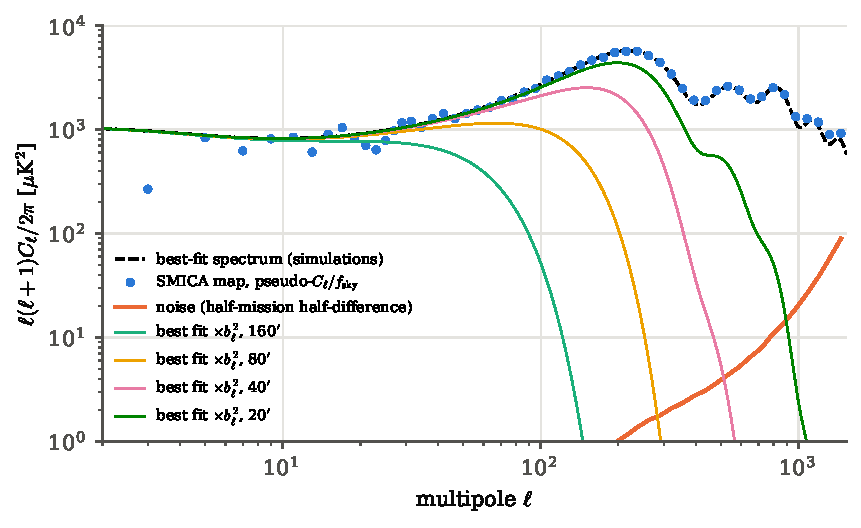
\includegraphics[width=0.82\linewidth]{figures/ch13/b_spectrum.pdf}
\caption{The power of the SMICA map against the spectrum used for the simulations. Blue points: the map's
pseudo-spectrum on the observed sky divided by $\fsky$, with the $5'$ beam and the pixel window removed; dashed:
the best-fit spectrum; orange: the noise from the half-difference map. The four thin curves are the best fit
multiplied by the squared working beams: each working map sees only the multipoles under its curve, where the
noise is far below the signal.}
\label{13b:fig:spectrum}
\end{figure}

\subsection{Does the map have the power of the simulations?}
\label{13b:sec:power}

The simulations are drawn from the best-fit spectrum of \cref{ch:T1}. If the map's power differed from it
substantially, the test would compare skies of different amplitude, and could fail for that reason alone. The
check in \cref{13b:fig:spectrum} is rough (the binary mask couples multipoles, \cref{8b:sec:coupling}, which the MASTER
estimator of \cref{8b:sec:master} would undo), but it is enough to see three things. Over $30\le\ell<800$,
which carries almost all the variance of our working maps, the ratio of the map's power to the best fit is
$\BpowMid$. Over $800\le\ell<1500$ it is $\BpowHigh$, and $\BpowHighNoNoise$ once the noise power is subtracted;
the remaining few per cent are the leakage of large-scale power through the edges of an unsoftened mask and the
residual point sources that \textit{Planck} also sees in the data and not in its simulations \cite{Planck2018VII}.
And over $2\le\ell<30$ the ratio is $\BpowLow$: the sky has less large-angle power than the best fit predicts. This is
the well-known low-variance anomaly of the largest scales (\cref{T3a:sec:anomalies}), and it will show up again
below as a smaller $\sigma_0$ of the real map at $160'$.

Does a power mismatch spoil the test? Not much, by construction. The thresholds are in units of the map's
\emph{own} standard deviation, so a sky that is uniformly too faint or too bright gives the same excursion sets
(\cref{12a:sec:monotone}); and the functionals are divided by the map's own $(\sigma_1/\sigma_0)^k$, which absorbs
most of a change in the spectrum's shape (\cref{12a:sec:planck}). What survives this normalisation is the shape of
the curves, which is what Gaussianity predicts.

\begin{figure}[htbp]
\centering
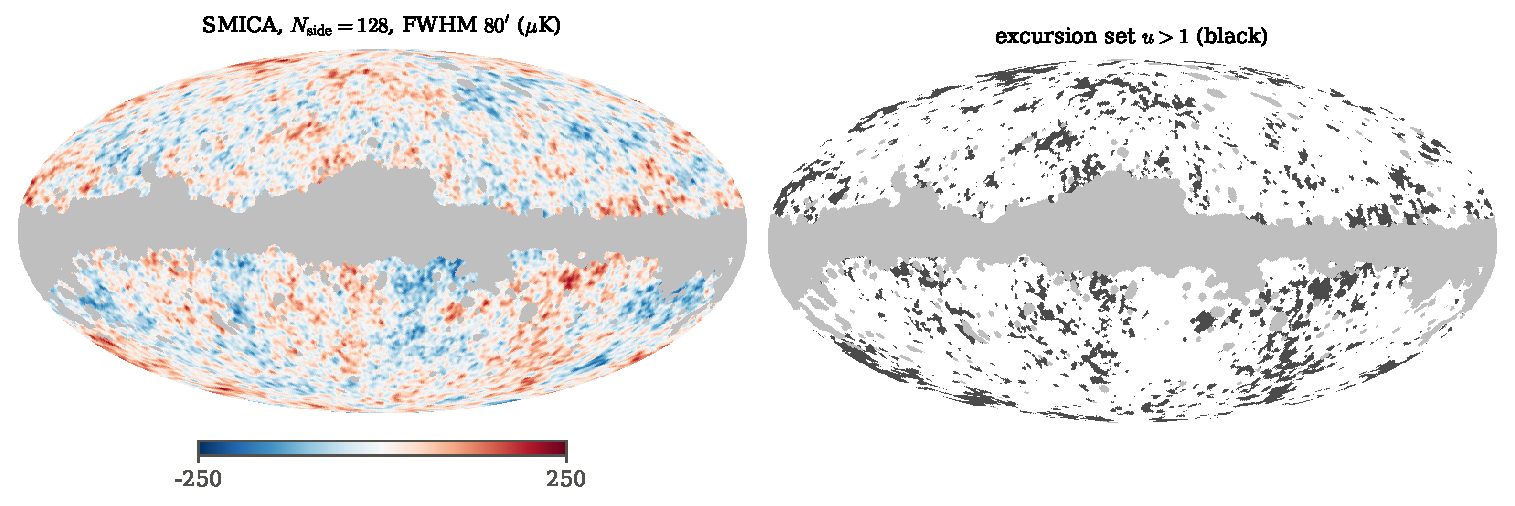
\includegraphics[width=\linewidth]{figures/ch13/b_maps.pdf}
\caption{The working map at $N_{\rm side}=128$ with an $80'$ beam (left), outside the degraded common mask (grey),
and its excursion set at one standard deviation (right): the observed pixels with $u=(T-\bar T)/\sigma_0>1$.
Every statistic below is a count or a measure of shapes like these, at twelve thresholds and four
resolutions.}
\label{13b:fig:maps}
\end{figure}
\section{The area, boundary and Euler characteristic of the real sky}
\label{13b:sec:mfs}

The working maps of \cref{13b:sec:data} are ready: four resolutions, each with its mask of observed pixels. At
each resolution we now ask the questions of \cref{ch:12} of the real sky. Standardise the map on its observed
pixels, $u=(T-\bar T)/\sigma_0$, with $\bar T$ and $\sigma_0$ the mean and the standard deviation over those
pixels only. For a threshold $\nu$, the excursion set $X_\nu$ is the set of observed pixels with $u>\nu$, the
hot regions of \cref{13b:fig:maps}. How much of the observed sky does it cover? How long is its boundary? How many
pieces does it have, minus how many holes? Each answer must come from code that a simulated sky passes through
unchanged, and each needs one decision about pixels that the formulas of \cref{12a:sec:gkf} never had to make.

\subsection{Three estimators on a cut sphere}
\label{13b:sec:estimators}

\paragraph{Area.} The fraction of observed pixels with $u>\nu$. HEALPix pixels all have the same area, so
counting them is measuring area, and $v_0(\nu)$ is this fraction.

\paragraph{Boundary length, without drawing a contour.} Tracing the contours $u=\nu$ through a pixelised map and
adding up their lengths is fiddly, especially where they run into the mask. There is a shortcut. \emph{The
question:} how is the length of a contour related to the area of a thin band around it? Take the band of points
where $u$ lies within $\Delta\nu/2$ of $\nu$. Near a point of the contour, $u$ changes fastest across the contour,
at the rate $|\nabla u|$ per radian, so the band there is $\Delta\nu/|\nabla u|$ wide. A short piece of contour of
length $\dd s$ therefore carries a strip of band of area $\dd A=\dd s\,\Delta\nu/|\nabla u|$. Solving for $\dd s$
and adding up the pieces,
\begin{align}
  L(\nu)
  &\eqby{1}\int_{u=\nu}\dd s
   \eqby{2}\lim_{\Delta\nu\to0}\frac{1}{\Delta\nu}\int_{|u-\nu|<\Delta\nu/2}|\nabla u|\,\dd A
   \eqby{3}\frac{A_{\rm obs}}{\Delta\nu}\,\Bigl\langle|\nabla u|\,\mathbb 1\bigl(|u-\nu|<\tfrac{\Delta\nu}{2}\bigr)\Bigr\rangle_{\rm obs}.
  \label{13b:eq:coarea}
\end{align}
\begin{explain}
  \item The length is the integral of the arc-length element along the contour.
  \item Each piece of contour, $\dd s=|\nabla u|\,\dd A/\Delta\nu$, comes with the piece of band beside it, so
        the integral over the contour becomes an integral over the band (this is the coarea formula, here in its
        simplest form).
  \item On equal-area pixels an integral over the observed sky is $A_{\rm obs}$ times the average over observed
        pixels; $\mathbb 1(\cdot)$ is $1$ inside the band and $0$ outside.
\end{explain}
The gradient comes exactly from the harmonic coefficients (\pyname{healpy.alm2map_der1} returns
$\partial_\theta u$ and $\partial_\phi u/\sin\theta$), so no finite differences are needed; we use
$\Delta\nu=0.1$. \textit{Planck}'s $V_1$ is a quarter of the length per unit area (their eq.~14), and we follow that
convention: $v_1=L/(4A_{\rm obs})$.

\paragraph{Example: the band estimator on a straight contour.} Take $u=k\,x$ on a flat patch of side $a$, a field
that rises steadily in one direction. The contour $u=\nu$ is the straight line $x=\nu/k$, of length $a$. The band
$|u-\nu|<\Delta\nu/2$ is the strip $|x-\nu/k|<\Delta\nu/(2k)$, of area $a\,\Delta\nu/k$, and in it $|\nabla u|=k$.
Then \eqref{13b:eq:coarea} gives $k\cdot a\,\Delta\nu/k/\Delta\nu=a$, the right answer for any slope: a steep field
has a thin band but a large gradient, and the two compensate exactly.

\paragraph{The Euler characteristic, at every threshold at once.} \Cref{12a:sec:vef} computed $\chi$ of a union of
closed pixels as $V-E+F$: vertices minus edges plus faces of the union. On the cut sphere we keep that rule and
add one: an unobserved pixel never belongs to the set. \emph{The question:} at which threshold does a given
vertex, edge or face join the union? A face (a pixel) joins when $\nu$ drops below its value. An edge or a vertex
belongs to the union as soon as \emph{one} of the observed pixels around it does, so it joins when $\nu$ drops
below the largest observed value around it. Every element thus has an entry level, and
\begin{equation}
  \chi(\nu)=\#\{\text{vertices entered above }\nu\}-\#\{\text{edges entered above }\nu\}+\#\{\text{faces entered above }\nu\}.
  \label{13b:eq:chi-levels}
\end{equation}
Sorting the three lists of entry levels once turns every $\chi(\nu)$ into three binary searches, which is how
\pyname{entry_levels} and \pyname{chi_from_levels} in \pyname{code/ch13/lib_skytopo.py} work. On full-sky
maps the result agrees exactly, threshold by threshold, with the pixel-by-pixel counter of \cref{ch:12}.

\paragraph{Example: four pixels by hand.} A $2\times2$ block of pixels has values $3$ (top left), $1$ (top right),
$0$ (bottom left) and $2$ (bottom right): $9$ vertices, $12$ edges, $4$ faces. Lower the threshold to $\nu=1.5$.
The faces above it are the top-left and bottom-right pixels, which touch only at the central vertex. Entry
levels: the central vertex sees all four values, so it joins at $\max(3,1,0,2)=3$; every other corner of the
top-left pixel has that pixel among its neighbours and joins at $3$, every other corner of the bottom-right pixel
joins at $2$ or $3$; an edge of either pixel joins at the larger of its two neighbouring values, at least $2$; and
every remaining vertex and edge touches only the pixels with values $1$ and $0$, so it joins below $1.5$. Counting
the elements that joined above $1.5$: $V=4+4-1=7$ (the central vertex is shared), $E=4+4=8$, $F=2$, so
$\chi=7-8+2=1$. The two diagonal pixels form one piece, because closed pixels that share a corner touch. This
is the convention of \cref{12a:sec:pixels} (hot pixels connect through corners, cold ones only through edges),
and \eqref{13b:eq:chi-levels} implements it automatically.

\paragraph{Normalisation.} As in \cref{12a:sec:planck}, the functionals are divided by the power of
$\sigma_1/\sigma_0$ that carries their dependence on the spectrum, with $\sigma_1^2$ the mean of $|\nabla T|^2$ over
the observed pixels: $v_1$ by $\sigma_1/\sigma_0$, and the Euler characteristic per steradian of observed sky,
$v_2=\chi/A_{\rm obs}$, by $(\sigma_1/\sigma_0)^2$. On the cut sky $v_2$ is not the Gaussian curve of
\eqref{12a:eq:planck-norm} alone: the mask's own topology and its boundary add the terms $\mathcal L_0\Psi(\nu)$ and
$\mathcal L_1\rho_1(\nu)$ of \cref{12a:sec:mask}. The simulations are cut by the same mask and carry the same terms,
so nothing has to be modelled.

\subsection{What the real sky gives}
\label{13b:sec:mf-results}

\paragraph{Example: one threshold, read off the sky.} At $N_{\rm side}=256$ and $\nu=\ExNu$ (one of \textit{Planck}'s twelve
thresholds), the excursion set of the SMICA map has $\ExBzeroData$ separate hot regions and $\ExBoneData$ holes in them,
so $\chi=\ExChiData$. The simulated skies, cut and processed identically, give $\chi=\ExChiMean$ on average with a
spread of $\ExChiSd$ from sky to sky. The real sky lies $(\ExChiData-\ExChiMean)/\ExChiSd\approx1.3$ standard deviations above the
mean, a deviation that about one Gaussian sky in five exceeds in one direction or the other. A single number like this is
easy to read, and also easy to over-read: there are $36$ such numbers per resolution, and they are not independent.

\Cref{13b:fig:mf-curves} shows the three normalised curves at $N_{\rm side}=256$ for the data and for the
simulations; \cref{13b:fig:mf-resid} shows, at all four resolutions, each number's deviation from the simulated mean
in units of the simulated standard deviation, $\Delta v/\sigma$. Three things stand out. First, the real sky's
curves lie inside the band of Gaussian skies everywhere, at every resolution; the largest single deviation is
$\MfMaxDevSixFour$, $\MfMaxDevOneTwoEight$, $\MfMaxDevTwoFiveSix$ and $\MfMaxDevFiveOneTwo$ standard deviations at
$N_{\rm side}=64$, $128$, $256$ and $512$. Second, the deviations mostly change smoothly with $\nu$: neighbouring
thresholds tend to move together, because the excursion sets at $\nu$ and at $\nu+0.55$ share most of their pixels. That
smoothness is the correlation we will have to take into account. Third, no curve stays at zero: each wanders up and
down by about one standard deviation, at every resolution. That is what a single realisation does. At
$N_{\rm side}=64$ the observed sky holds only a few hundred independent patches, so a slight surplus of hot area
at some thresholds and a deficit at others is expected, not a sign of anything.

\begin{figure}[htbp]
\centering
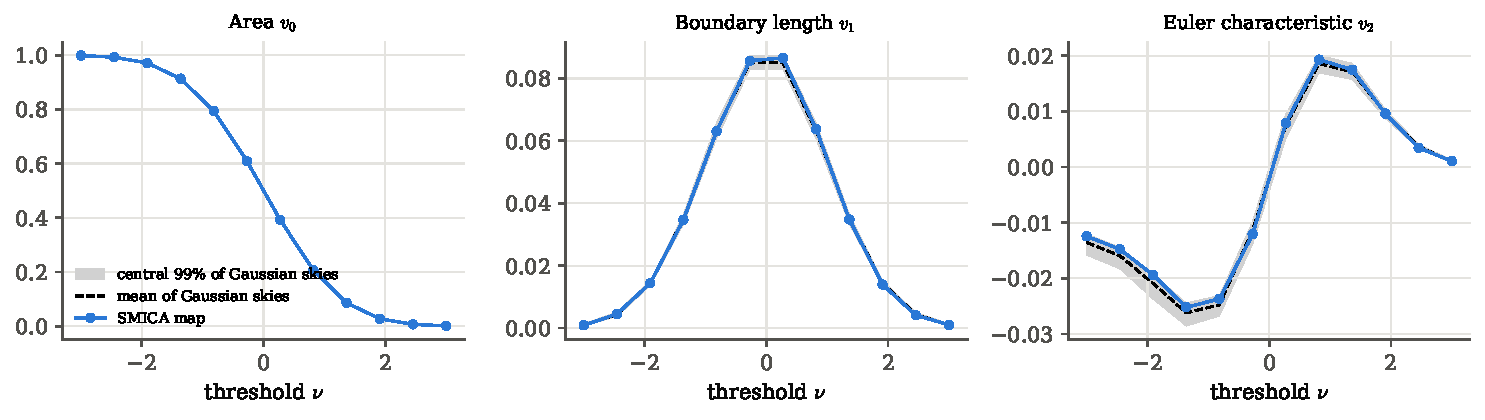
\includegraphics[width=\linewidth]{figures/ch13/b_mf_curves.pdf}
\caption{The three normalised Minkowski functionals of the SMICA map at $N_{\rm side}=256$ ($40'$), against $\MfNTwoFiveSix$
Gaussian skies with the best-fit spectrum, the same beam, pixels, noise and mask. Grey: the central $99\%$ of the
skies; dashed: their mean. The genus curve is asymmetric about zero because of the mask: its boundary and its
holes add pieces to every excursion set.}
\label{13b:fig:mf-curves}
\end{figure}

\paragraph{The amplitude that was divided out.} The normalisation removed $\sigma_0$ and $\sigma_1/\sigma_0$; it is
worth looking at them directly, because they are where the spectrum lives. The real map's $\sigma_0$ is
$\SzeroDataSixFour$, $\SzeroDataOneTwoEight$, $\SzeroDataTwoFiveSix$ and $\SzeroDataFiveOneTwo\,\mu$K at the four
resolutions; the Gaussian skies give $\SzeroSimSixFour\pm\SzeroSdSixFour$, $\SzeroSimOneTwoEight\pm\SzeroSdOneTwoEight$,
$\SzeroSimTwoFiveSix\pm\SzeroSdTwoFiveSix$ and $\SzeroSimFiveOneTwo\pm\SzeroSdFiveOneTwo\,\mu$K. Only
$\SzeroRankSixFour\%$ of the skies have a $\sigma_0$ as small as the data at $160'$: the deficit of large-angle power
found in \cref{13b:sec:power}, now as a variance. The ratio $\sigma_1/\sigma_0$ is $\RatioDataTwoFiveSix$ per radian
in the data at $N_{\rm side}=256$, against $\RatioSimTwoFiveSix\pm\RatioSdTwoFiveSix$ in the skies. Had we compared the
unnormalised functionals, or set the thresholds in units of the simulations' average $\sigma_0$, the low variance
would have shifted every curve and been mistaken for a change of shape. The normalisation keeps the two questions
apart: ``is the amplitude typical?'' is a question about the power spectrum, and ``is the shape Gaussian?'' is the
question asked here.

\begin{figure}[htbp]
\centering
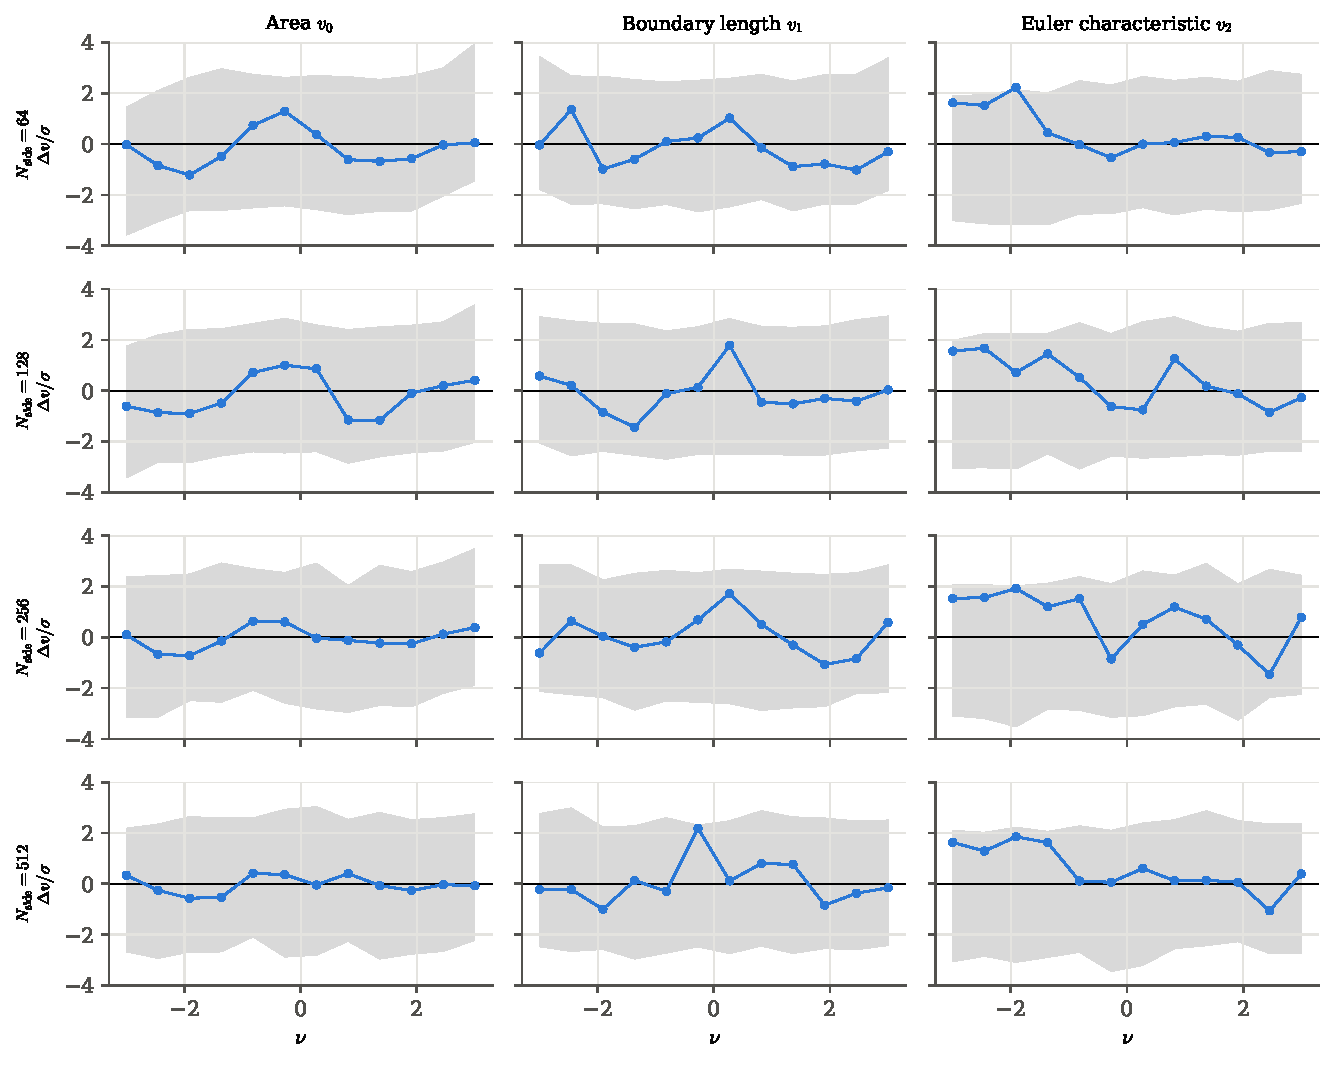
\includegraphics[width=0.95\linewidth]{figures/ch13/b_mf_resid.pdf}
\caption{Deviation of each of the $36$ numbers of the SMICA map from the mean of the Gaussian skies, in units of
their standard deviation, at the four resolutions (rows). Grey: the central $99\%$ of the skies, each measured
the same way. Neighbouring thresholds move together, which is why the $36$ deviations cannot be judged one at a
time.}
\label{13b:fig:mf-resid}
\end{figure}

\begin{pitfall}[looking for the largest deviation]
With $36$ numbers per resolution and four resolutions, the largest of $144$ deviations of a Gaussian sky is
typically well beyond two standard deviations, even though each single number exceeds two standard deviations
only $5\%$ of the time. A deviation found by scanning a figure must be judged against the largest deviation of the
simulations scanned in the same way, not against the normal distribution: this is the look-elsewhere effect of
\cref{ch:04}. The $\chi^2$ of \cref{13b:sec:chi2} avoids the problem by fixing in advance one number per
resolution.
\end{pitfall}
\section{Thirty-six numbers, one verdict}
\label{13b:sec:chi2}

\Cref{13b:fig:mf-resid} shows $36$ deviations per resolution, all modest, all moving together with their
neighbours. How surprised should we be by the whole pattern? Adding up the squared deviations would count the
same fluctuation many times, once for every threshold it touches; picking the largest one invites the
look-elsewhere trap. We need one number per resolution that measures how far the vector $\bm y_{\rm obs}$ lies
from the Gaussian average, counting each independent fluctuation once, and then the distribution of that number
under the null hypothesis of \cref{13b:sec:question}.

\subsection{The distance that the null hypothesis itself defines}
\label{13b:sec:mahalanobis}

\paragraph{The question.} Among all the vectors $\bm y$ that Gaussian skies can produce, which ones count as
``farther from the average than ours''? The natural answer is: those that the null hypothesis makes \emph{less
probable} than ours. To use it we need the density of $\bm y$ under the null.

\emph{The density.} Each component of $\bm y$ is an average over the observed sky: a fraction of pixels, a
length per area, a count per area. The observed sky contains many patches a correlation length apart, and their
contributions are nearly independent, so by the central limit theorem (\cref{ch:02}) the vector is close to a
multivariate Gaussian with some mean $\bm\mu$ and covariance $\Cmat$:
\begin{equation}
  p(\bm y\given\Hnull)\approx\frac{1}{\sqrt{(2\pi)^{p}\det\Cmat}}\exp\Bigl[-\frac12(\bm y-\bm\mu)\T\Cmat^{-1}(\bm y-\bm\mu)\Bigr],
  \label{13b:eq:mvn}
\end{equation}
with $p=36$ components. The density depends on $\bm y$ only through the quadratic form in the exponent, and falls
as it grows. So ``less probable than ours'' is the same as ``a larger value of
$Q(\bm y)=(\bm y-\bm\mu)\T\Cmat^{-1}(\bm y-\bm\mu)$''. The surfaces of constant $Q$ are ellipsoids aligned with the
correlations: a deviation along a direction in which the skies naturally fluctuate a lot costs little, a deviation
in a direction they rarely take costs much. And if $\bm\mu$ and $\Cmat$ were known exactly, $Q$ would follow the
$\chi^2$ distribution with $p$ degrees of freedom (\cref{2b:sec:chi2-quadform}): mean $36$, standard deviation
$\sqrt{72}\approx8.5$, the scale of a $\chi^2$ with $36$ components that \cref{T3a:sec:planck-mf} already met.

\paragraph{Example: why correlated thresholds must not be added as if independent.} Take two thresholds whose
deviations, in units of their standard deviations, have correlation $\rho$, and suppose both came out at $+1$.
With $\Cmat=\bigl(\begin{smallmatrix}1&\rho\\ \rho&1\end{smallmatrix}\bigr)$,
\begin{align*}
  Q
  &\eqby{1}\frac{1}{1-\rho^2}\,(1,\ 1)\begin{pmatrix}1&-\rho\\-\rho&1\end{pmatrix}\begin{pmatrix}1\\1\end{pmatrix}
   \eqby{2}\frac{2-2\rho}{1-\rho^2}
   \eqby{3}\frac{2}{1+\rho}.
\end{align*}
\begin{explain}
  \item The inverse of a $2\times2$ matrix: swap the diagonal, negate the off-diagonal, divide by the determinant
        $1-\rho^2$.
  \item Multiply out: $1-\rho-\rho+1$.
  \item $1-\rho^2=(1-\rho)(1+\rho)$, and $1-\rho$ cancels.
\end{explain}
For independent thresholds ($\rho=0$) the two deviations count twice, $Q=2$. For $\rho=0.9$, the strongest
correlation between neighbouring area thresholds in \cref{13b:fig:corr} (most neighbouring pairs lie between
$0.5$ and $0.9$), $Q=1.05$: two deviations that the skies
almost always make together are worth hardly more than one. Had the second deviation come out at $-1$ instead,
$Q=2/(1-\rho)=20$: a pattern that cuts across the correlation is very improbable, even though each number on its
own is ordinary. The quadratic form sees both effects.

\begin{figure}[htbp]
\centering
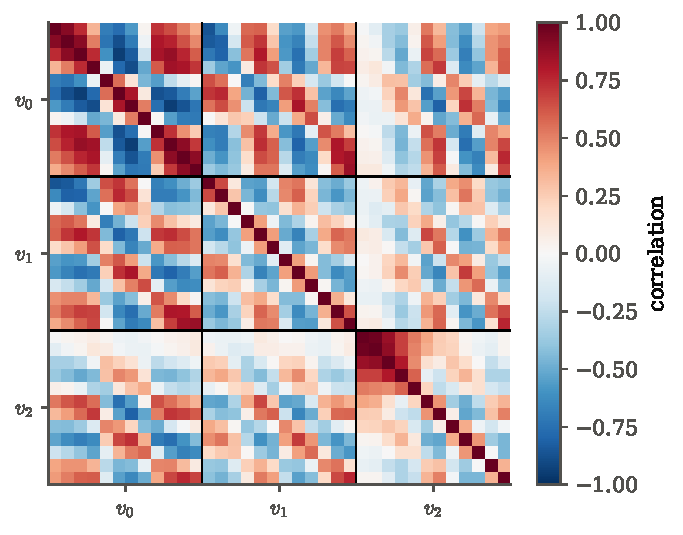
\includegraphics[width=0.55\linewidth]{figures/ch13/b_corr.pdf}
\caption{Correlation matrix of the $36$ numbers at $N_{\rm side}=256$, estimated from the Gaussian skies. Blocks:
area, length and Euler characteristic, each at twelve thresholds from $-3$ to $3$. Each sky is measured in units
of its own mean and rms, so its areas cannot all grow together: the area fractions at the tail thresholds
($|\nu|>1$) move together, and against those in the core ($|\nu|<1$). Neighbouring area thresholds on the same side
of $|\nu|=1$ are correlated at $0.5$ to $0.9$; the two pairs that straddle it hardly at all. Length and Euler
characteristic are less tightly tied, but many entries far from the diagonal still reach $\pm0.5$ or more.}
\label{13b:fig:corr}
\end{figure}

\subsection{When the mean and covariance come from simulations}
\label{13b:sec:hartlap}

We do not know $\bm\mu$ and $\Cmat$; we estimate them from $n$ simulated skies, $\bar{\bm y}$ and
$\widehat{\Cmat}$. Two corrections follow, both from \cref{ch:03}.

\emph{The inverse of a noisy covariance is biased.} $\widehat{\Cmat}$ is unbiased, but its inverse is not: random
errors make some directions look less variable than they are, and $\widehat{\Cmat}^{-1}$ inflates them.
For Gaussian vectors, $\E\,\widehat{\Cmat}^{-1}=\frac{n-1}{n-p-2}\,\Cmat^{-1}$ \eqref{3a:eq:hartlap}, so the
unbiased estimate of the inverse is $h\,\widehat{\Cmat}^{-1}$ with the Hartlap factor $h=(n-p-2)/(n-1)$
\cite{Hartlap2007}. With $\MfNTwoFiveSix$ skies at $N_{\rm side}=256$ it is $\MfHartTwoFiveSix$; with
$\MfNFiveOneTwo$ skies at $N_{\rm side}=512$ it is $\MfHartFiveOneTwo$. That is the factor $h$ in \eqref{13b:eq:chi2}.

\emph{A simulation must not judge itself.} To get the null distribution of $\chi^2$ we compute it for every
simulated sky. If sky $i$ were included in the mean and covariance it is compared with, it would pull both
towards itself and look too typical. How much too typical? Sum the uncorrected quadratic forms of all $n$ skies,
with $\bm d_i=\bm y_i-\bar{\bm y}$ and $\widehat{\Cmat}=\frac1{n-1}\sum_j\bm d_j\bm d_j\T$:
\begin{align}
  \sum_{i=1}^n\bm d_i\T\widehat{\Cmat}^{-1}\bm d_i
  &\eqby{1}\sum_{i=1}^n\tr\bigl(\widehat{\Cmat}^{-1}\bm d_i\bm d_i\T\bigr)
   \eqby{2}\tr\Bigl(\widehat{\Cmat}^{-1}\sum_{i=1}^n\bm d_i\bm d_i\T\Bigr)
   \eqby{3}\tr\bigl(\widehat{\Cmat}^{-1}(n-1)\widehat{\Cmat}\bigr)
   \eqby{4}(n-1)\,p .
  \label{13b:eq:insample}
\end{align}
\begin{explain}
  \item A number equals its own trace, and $\tr(\mathbf A\mathbf B)=\tr(\mathbf B\mathbf A)$ moves $\bm d_i$ to the end.
  \item The trace is linear, so the sum goes inside.
  \item The definition of the sample covariance.
  \item $\tr\Id_p=p$.
\end{explain}
So the average in-sample value is $p(n-1)/n$, \emph{exactly}, whatever the skies did: slightly below $p$, with no
scatter in the average at all. A new, independent sky compared with the same $\bar{\bm y}$ and $\widehat{\Cmat}$ has
instead an average of about $p\,(n-1)/(n-p-2)$, above $p$. The data are a new sky in this sense, so each simulation
is treated the same way: its $\chi^2$ uses the mean and covariance of the \emph{other} $n-1$ skies (with Hartlap factor
$(n-p-3)/(n-2)$). This ``leave-one-out'' distribution is the null distribution the data are ranked in. Its mean,
$\MfSimMeanTwoFiveSix$ per degree of freedom at $N_{\rm side}=256$, confirms that the corrections work.

\emph{The Gaussian approximation is not used for the probability.} \Cref{13b:eq:mvn} told us which statistic to use.
It is not trusted for the tail: at $|\nu|=3$ the counts are small and skewed, and $\bar{\bm y}$ and $\widehat{\Cmat}$
carry their own noise. The probability is the rank \eqref{13b:eq:rank-p} of the data's $\chi^2$ among the
simulations' $\chi^2$, which needs no formula. The tail of the $\chi^2_{36}$ distribution is reported alongside, as a
check on how far the approximation can be trusted.

\begin{keyidea}[the simulation test of a sky map]
Stack the statistics into a vector. Use simulations of the null hypothesis, processed exactly like the data, to
estimate its mean and covariance; form the Hartlap-corrected $\chi^2$ of the data and, leaving each one out in
turn, of every simulation. The $p$-value is the fraction of simulations whose $\chi^2$ is at least as large as the
data's. The Gaussian density chooses the statistic; the simulations, not a formula, give its distribution.
\end{keyidea}

\subsection{The verdict at four resolutions}
\label{13b:sec:verdict}

The simulated skies are made and measured once, by \pyname{code/ch13/b02_sims.py}, and cached. The test itself is a
short function in \pyname{code/ch13/b03_mf_test.py}:
\pyfile[firstline=57,lastline=67]{code/ch13/b03_mf_test.py}{The $\chi^2$ of the data and the leave-one-out $\chi^2$ of every simulation}
\noindent The first four lines are \eqref{13b:eq:chi2} for the data, with the covariance of all $n$ skies; the
loop repeats it for each simulation against the other $n-1$. The rank \eqref{13b:eq:rank-p} is then one line,
\pyname{np.mean(c_sims >= c_data)}. \Cref{13b:tab:mf} collects the results.

\begin{table}[htbp]
\centering
\small
\begin{tabular}{lcccc}
\toprule
 & $N_{\rm side}=64$ & $128$ & $256$ & $512$\\
 & $160'$ & $80'$ & $40'$ & $20'$\\
\midrule
simulated skies $n$ & $\MfNSixFour$ & $\MfNOneTwoEight$ & $\MfNTwoFiveSix$ & $\MfNFiveOneTwo$\\
Hartlap factor $h$ & $\MfHartSixFour$ & $\MfHartOneTwoEight$ & $\MfHartTwoFiveSix$ & $\MfHartFiveOneTwo$\\
$\chi^2/N_{\rm dof}$ of the data & $\MfChiNSixFour$ & $\MfChiNOneTwoEight$ & $\MfChiNTwoFiveSix$ & $\MfChiNFiveOneTwo$\\
$\widehat p$ (rank among skies), \% & $\MfPSixFour\pm\MfPerrSixFour$ & $\MfPOneTwoEight\pm\MfPerrOneTwoEight$ & $\MfPTwoFiveSix\pm\MfPerrTwoFiveSix$ & $\MfPFiveOneTwo\pm\MfPerrFiveOneTwo$\\
tail of $\chi^2_{36}$, \% & $\MfPchiSixFour$ & $\MfPchiOneTwoEight$ & $\MfPchiTwoFiveSix$ & $\MfPchiFiveOneTwo$\\
area alone, \% & $\MfPAreaSixFour$ & $\MfPAreaOneTwoEight$ & $\MfPAreaTwoFiveSix$ & $\MfPAreaFiveOneTwo$\\
length alone, \% & $\MfPLengthSixFour$ & $\MfPLengthOneTwoEight$ & $\MfPLengthTwoFiveSix$ & $\MfPLengthFiveOneTwo$\\
Euler characteristic alone, \% & $\MfPGenusSixFour$ & $\MfPGenusOneTwoEight$ & $\MfPGenusTwoFiveSix$ & $\MfPGenusFiveOneTwo$\\
\midrule
\textit{Planck} 2018, SMICA, \% & $\MfPlanckPSixFour$ & $\MfPlanckPOneTwoEight$ & $\MfPlanckPTwoFiveSix$ & $\MfPlanckPFiveOneTwo$\\
\bottomrule
\end{tabular}
\caption{The Minkowski-functional test of the SMICA temperature map. $\widehat p$ is the fraction of Gaussian skies
with a $\chi^2$ at least as large as the data's, with its binomial Monte Carlo error; the three rows below use the
twelve numbers of one functional at a time. The last row is the same probability from \textit{Planck}'s Table~5
\cite{Planck2018VII}, with $999$ end-to-end simulations.}
\label{13b:tab:mf}
\end{table}

\begin{figure}[htbp]
\centering
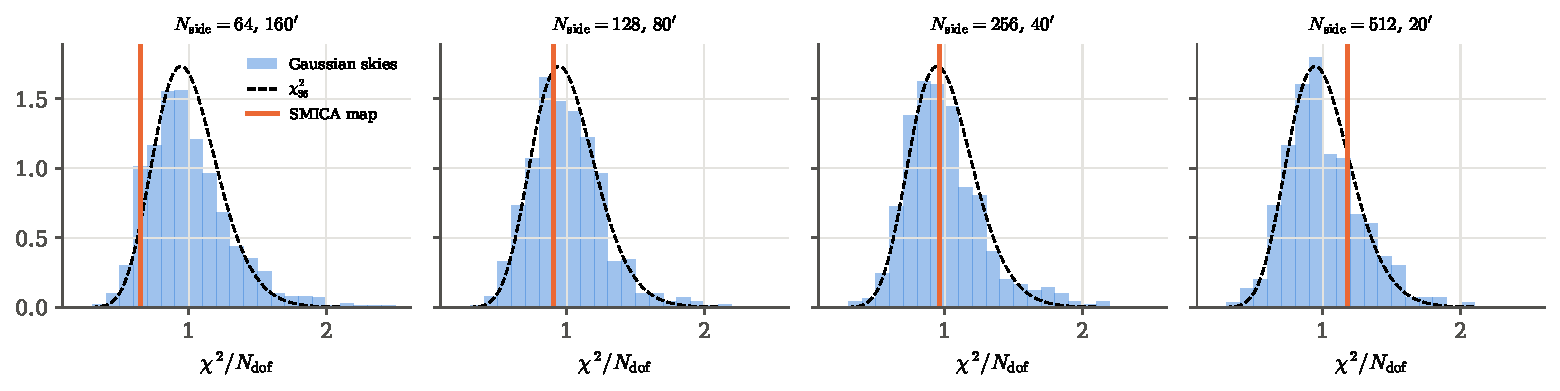
\includegraphics[width=\linewidth]{figures/ch13/b_chi2.pdf}
\caption{The $\chi^2$ per degree of freedom of each Gaussian sky against the others (histogram), the $\chi^2_{36}$
density (dashed), and the SMICA map (vertical line), at the four resolutions. The data sit inside the bulk of the
Gaussian skies at every resolution.}
\label{13b:fig:chi2}
\end{figure}

\paragraph{Reading the verdict.} Go back to the four candidate explanations of \cref{13b:sec:question}. The data's
$\chi^2$ lands in the bulk of the null distribution at every resolution (\cref{13b:fig:chi2}): between
$\MfPFiveOneTwo\%$ and $\MfPSixFour\%$ of Gaussian skies are farther from the Gaussian average than the real one.
So the first explanation, a Gaussian sky seen through our instrument, accounts for the shapes of the real sky
without strain, and the other three are not needed to explain these $36$ numbers. That is a statement about
sensitivity as much as about the sky: a primordial non-Gaussianity, a foreground residual or a processing error
smaller than the scatter of these statistics would pass unseen, and \cref{T3a:sec:planck-fnl} shows how much
tighter the bispectrum constrains the primordial kind.

\paragraph{One small number among twelve.} The single-functional rows matter because a defect in one estimator
(the boundary length near the mask, say) would show in one row and not in the others. Eleven of the twelve are
unremarkable; the boundary length at $N_{\rm side}=512$ gives $\MfPLengthFiveOneTwo\%$. Is that a sign of
something? Ask how often the smallest of twelve probabilities is that small when nothing is wrong. If the twelve were
independent, each below $\MfPsingleMin$ with probability $\MfPsingleMin$, the chance that none of them is would be
$(1-\MfPsingleMin)^{12}=\MfNoneBelow$; in all the other perfectly Gaussian skies at least one row is this small. The rows are
in fact correlated (the same sky enters all of them), which lowers that chance somewhat but not to anything rare.
This is the look-elsewhere effect again: the smallest probability was found by looking at twelve numbers, and it has to be judged as
the smallest of twelve. The combined test, fixed in advance, is the one that carries the verdict.
\section{Pieces, holes and their lifetimes on the real sky}
\label{13b:sec:betti}

The Euler characteristic of \cref{13b:sec:mfs} is a difference, pieces minus holes, $\chi=\beta_0-\beta_1$
(\cref{12a:sec:xnu}). A sky with ten more hot regions and ten more holes than a Gaussian one has the same $\chi$.
Could the real sky hide such a compensation? The Betti numbers separate the two counts, and the persistence
diagram of \cref{12b:sec:filtration} goes further: it follows each hot region from the threshold at which it
appears to the threshold at which it merges with an older one. Both were developed for cosmic-web catalogues
\cite{Pranav2017} and for primordial non-Gaussianity in galaxy surveys \cite{Biagetti2021}; here they are applied to
the real microwave sky, through the same simulation test.

\paragraph{The question.} Does the real sky have, threshold by threshold, the number of separate hot regions and
the number of holes in them that Gaussian skies have? And is the whole history of its hot regions, births and
mergers, as close to that of a Gaussian sky as Gaussian skies are to one another?

\subsection{Betti numbers on a cut sphere}
\label{13b:sec:betti-sphere}

\emph{Pieces.} $\beta_0(\nu)$, the number of connected hot regions, is computed by the union--find algorithm of
\cref{12b:sec:unionfind}, run on the HEALPix neighbour graph: the observed pixels are added in order of decreasing
$u$; each new pixel is joined to the observed neighbours already present (all neighbours, up to eight, that share an edge
or a corner, the convention of \cref{13b:sec:estimators}); when it joins two regions, the younger dies (the elder
rule). One pass gives the birth and death level of every hot region, and $\beta_0(\nu)$ is the number of regions
born above $\nu$ and not yet merged at $\nu$. In \pyname{code/ch13/lib_skytopo.py} the loop is compiled with
\pyname{numba}, and it handles the $3$ million pixels of an $N_{\rm side}=512$ map in $\HzeroTimeFiveOneTwo$\,s on one core of
the cluster, most of it spent following the eight neighbours of each pixel.

\emph{Holes, from pieces and the Euler characteristic.} Counting holes directly on a sphere with a mask is
awkward: is a cold region that touches the mask a hole or not? There is no need to decide. For a surface,
$\chi=\beta_0-\beta_1+\beta_2$, where $\beta_2$ counts closed two-dimensional shells. A subset of the sphere
contains a closed shell only if it is the whole sphere, and with a mask our excursion sets never are, so
$\beta_2=0$ and
\begin{equation}
  \beta_1(\nu)=\beta_0(\nu)-\chi(\nu),
  \label{13b:eq:b1}
\end{equation}
with $\chi$ from \eqref{13b:eq:chi-levels}. A hole is then whatever $\chi$ says it is: a cold region enclosed by hot
pixels, and also a hot region wrapped around one of the mask's holes. Both are features of the observed excursion
set, and the simulations see the same mask. As a check of the code, on unmasked skies Alexander duality gives
$\beta_1$ another way, as the number of cold regions (four-connected) minus one (\cref{12b:sec:lakes}, here on the
sphere instead of the plane). The script \pyname{code/ch13/b05_checks.py} makes this comparison on $\DualMaps$ full-sky
Gaussian maps at $N_{\rm side}=64$ and $128$, at $61$ thresholds each: of the $\DualCases$ cases in which both the hot
and the cold set are non-empty, $\DualBad$ disagree.

\paragraph{Example: the split of $\chi$ at one threshold.} At $N_{\rm side}=256$ and $\nu=\ExNu$ the real sky has
$\beta_0=\ExBzeroData$ hot regions and $\beta_1=\ExBoneData$ holes, so that $\chi=\ExBzeroData-\ExBoneData=\ExChiData$
(\cref{13b:sec:mf-results}). Near $\nu=0$ hot and cold areas are about equal and both counts are large; the Euler
characteristic, their small difference, has a relative scatter much larger than either count. The Betti numbers
are therefore not redundant with $\chi$: they measure the two large numbers that $\chi$ subtracts.

\paragraph{The test.} The statistics vector now holds $\beta_0$ and $\beta_1$ per steradian of observed sky at the
twelve thresholds, $24$ numbers per resolution. A threshold at which no simulated sky varied (if no sky ever had a
hole in its hot set at $\nu=3$, for example) would carry no information and would have to be dropped, since its
row of the covariance would be zero; the script checks this, and at our four resolutions all $24$ numbers vary. The
test of \cref{13b:sec:chi2} then runs unchanged.
The SMICA map gives
\begin{center}
\small
\begin{tabular}{lcccc}
\toprule
 & $N_{\rm side}=64$ & $128$ & $256$ & $512$\\
\midrule
numbers used & $\BeDofSixFour$ & $\BeDofOneTwoEight$ & $\BeDofTwoFiveSix$ & $\BeDofFiveOneTwo$\\
$\chi^2/N_{\rm dof}$ & $\BeChiNSixFour$ & $\BeChiNOneTwoEight$ & $\BeChiNTwoFiveSix$ & $\BeChiNFiveOneTwo$\\
$\widehat p$, \% & $\BePSixFour\pm\BePerrSixFour$ & $\BePOneTwoEight\pm\BePerrOneTwoEight$ & $\BePTwoFiveSix\pm\BePerrTwoFiveSix$ & $\BePFiveOneTwo\pm\BePerrFiveOneTwo$\\
\bottomrule
\end{tabular}
\end{center}
with the curves in \cref{13b:fig:betti}. As with the functionals, the real sky's pieces and holes are where Gaussian
skies put them.

\begin{figure}[htbp]
\centering
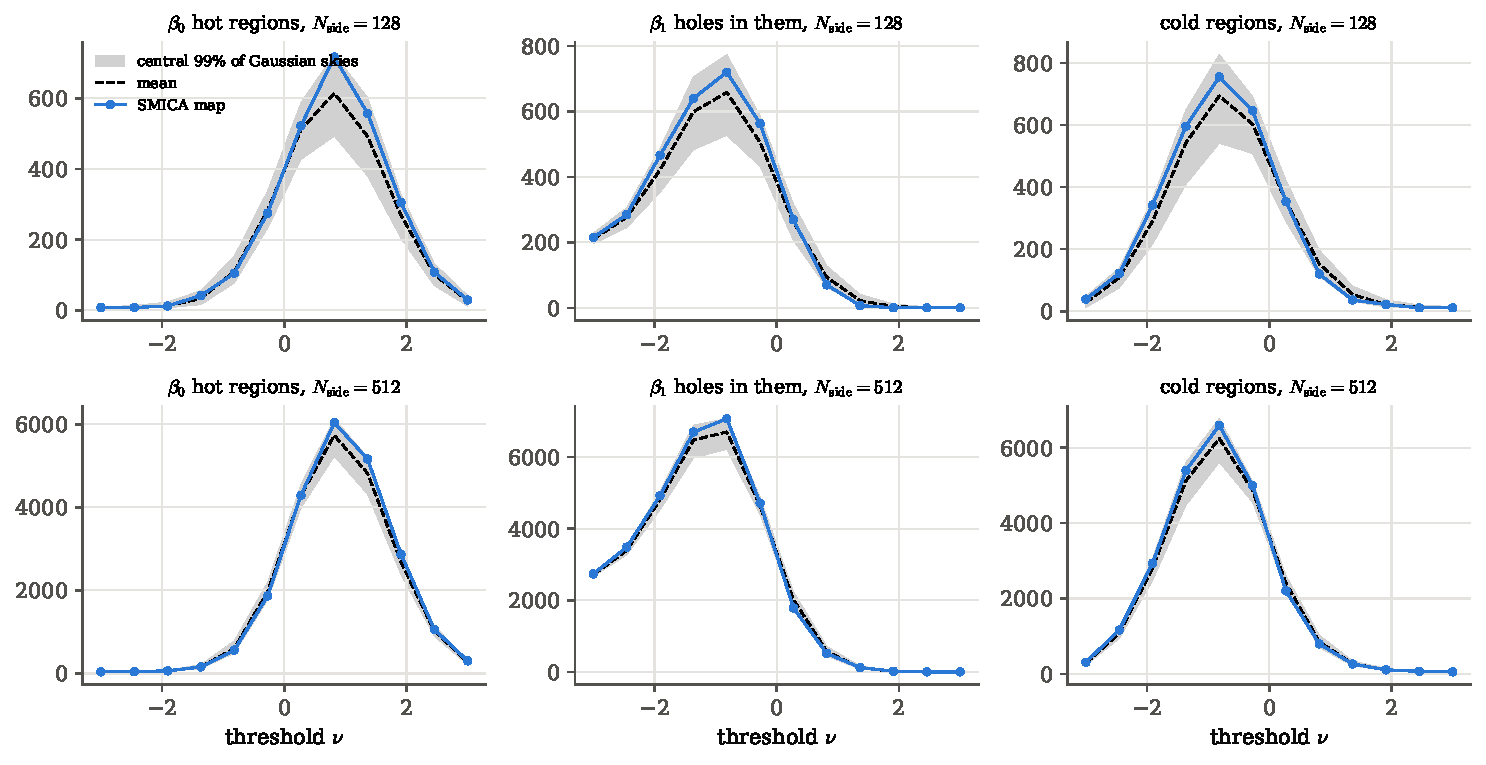
\includegraphics[width=\linewidth]{figures/ch13/b_betti.pdf}
\caption{Betti curves of the SMICA map (blue) at $N_{\rm side}=128$ ($80'$, top) and $512$ ($20'$, bottom): the number of
hot regions $\beta_0$, the number of holes in them $\beta_1=\beta_0-\chi$, and the number of cold regions, against
the central $99\%$ (grey) and the mean (dashed) of the Gaussian skies. The counts are totals over the observed sky.}
\label{13b:fig:betti}
\end{figure}

\subsection{The whole history: persistence diagrams}
\label{13b:sec:persistence}

The same union--find pass that counts $\beta_0$ records, for every hot region, a pair (birth level, death level).
Plotted as points, these pairs form the $H_0$ persistence diagram of the map (\cref{12b:sec:filtration}): a point far
from the diagonal is a hot spot that stood out over a wide range of thresholds, a point near the diagonal a
blip. Two features of the cut sky are worth naming. A region cut off from the rest of the observed sky by the mask
can never merge with it, so the diagram has one never-dying point for each separate island of observed sky; these
carry information about the mask, not the sky, and are left out. And the levels are in units of the map's own
$\sigma_0$, so the diagram, like the curves, is insensitive to the overall amplitude.

\paragraph{Comparing a diagram with a population of diagrams.} A diagram is a set of points, not a vector, so the
$\chi^2$ of \cref{13b:sec:chi2} does not apply directly; nor is there a simple ``mean diagram'' of the Gaussian skies
to compare with. What we do have is a distance. The $1$-Wasserstein distance $W_1$ (\cref{12b:sec:bottleneck})
matches the points of two diagrams one to one, sending unmatched points to the diagonal, and adds up the costs of
the best matching; each cost is the larger of the shifts in birth and in death, and the cost of a point sent to
the diagonal is half its lifetime.

\paragraph{Example: $W_1$ by hand.} Let $D=\{(2,0.5)\}$ and $D'=\{(2.2,0.4),\,(0.3,0.2)\}$. Matching
$(2,0.5)$ with $(2.2,0.4)$ and sending $(0.3,0.2)$ to the diagonal costs
\begin{align*}
  \max(|2-2.2|,|0.5-0.4|)+\frac{0.3-0.2}{2}
  &= 0.2+0.05=0.25 ,
\end{align*}
while sending everything to the diagonal costs $\frac{1.5}{2}+\frac{1.8}{2}+\frac{0.1}{2}=1.7$, and matching $(2,0.5)$
with $(0.3,0.2)$ is worse still. So $W_1(D,D')=0.25$: the long-lived spot moved by $0.2$, and one short blip was
created. Unlike the bottleneck distance, which keeps only the worst pair, $W_1$ adds up every change, so a sky with
many slightly displaced spots is far from a Gaussian one even when no single spot moved much.

\paragraph{Computing the best matching.} Finding the cheapest matching looks like a search over all pairings, but
it is a standard problem in disguise. \emph{The trick:} give every point a private copy of itself on the
diagonal. If $D$ has $n$ points and $D'$ has $m$, list as ``rows'' the $n$ points of $D$ followed by the $m$
diagonal copies of the points of $D'$, and as ``columns'' the $m$ points of $D'$ followed by the $n$ diagonal copies
of the points of $D$. A row--column pair is then one of four things: a point of $D$ matched to a point of $D'$ (cost:
the larger shift), a point of $D$ sent to its own diagonal copy (cost: half its lifetime), a point of $D'$ sent to
its diagonal copy (the same), or two diagonal copies paired with each other (cost $0$, nothing happens). Every
matching of the two diagrams is a one-to-one assignment of the $n+m$ rows to the $n+m$ columns, and the cheapest
assignment of a square cost matrix is what \pyname{scipy.optimize.linear_sum_assignment} computes exactly (the
Hungarian algorithm). The function \pyname{w1} in \pyname{code/ch13/b04_betti_persistence.py} builds this matrix in
five lines, and on the example above it returns $\WdExample$. Research code uses \pyname{gudhi}'s
\pyname{hera.wasserstein_distance} (order $1$, ground metric $L^\infty$), which solves the same problem with a faster
approximate auction algorithm.

\paragraph{The test statistic.} For each map we compute its mean $W_1$ distance to a fixed set of reference skies
($\WdNrefSixFour$ Gaussian skies at $N_{\rm side}=64$, $\WdNrefOneTwoEight$ at $128$). Before matching, points that
live less than $\WdCutSixFour\,\sigma_0$ (at $64$) or $\WdCutOneTwoEight\,\sigma_0$ (at $128$) are dropped. They are
the many tiny wiggles of the field, each costing almost nothing, and they make the cost matrix large (the matching
time grows as the cube of the number of points) without adding information about the long-lived spots. A Gaussian sky
is at a typical distance from the references; a non-Gaussian one, whose spots are born and merge at the wrong levels,
would be farther. The null distribution comes from $\WdNtestSixFour$ and $\WdNtestOneTwoEight$ further Gaussian skies,
not among the references, and the $p$-value is again the rank of the data. At $N_{\rm side}=128$ the SMICA diagram
keeps $\WdPtsDataOneTwoEight$ points after the cut (a Gaussian sky about $\WdPtsSimOneTwoEight$). Its mean distance to
the references is $\WdDataOneTwoEight$, against
$\WdSimOneTwoEight\pm\WdSdOneTwoEight$ for Gaussian skies, so $\WdPOneTwoEight\%$ of Gaussian skies are farther; at
$N_{\rm side}=64$ the numbers are $\WdDataSixFour$ against $\WdSimSixFour\pm\WdSdSixFour$, and $\WdPSixFour\%$
(\cref{13b:fig:persistence}).

\begin{figure}[htbp]
\centering
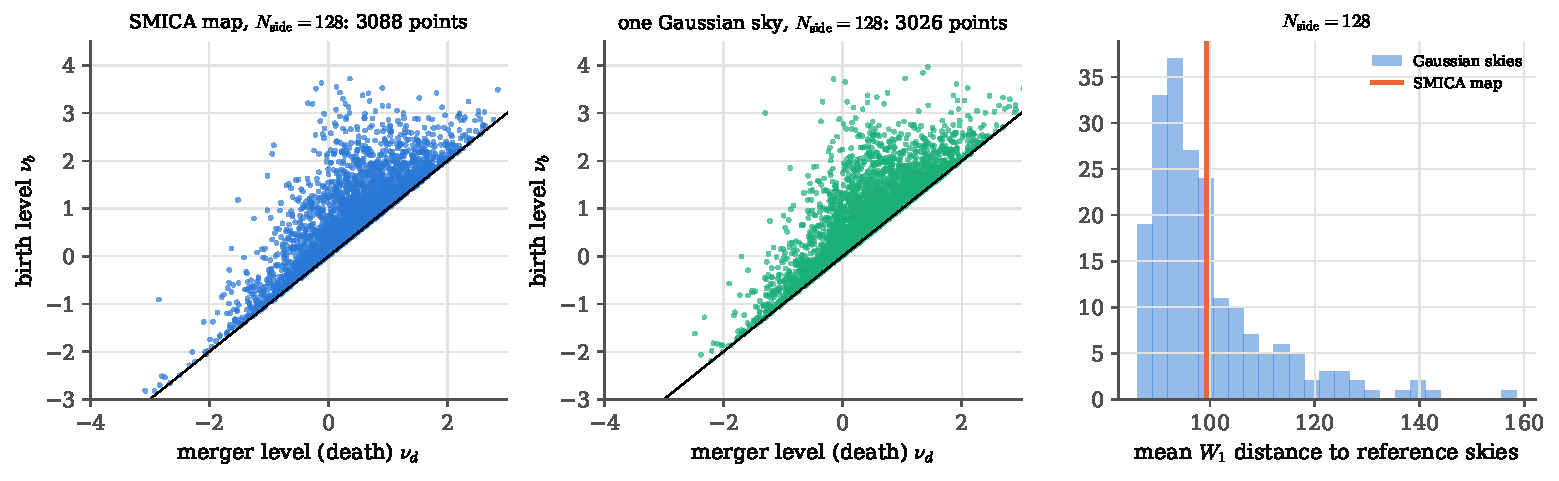
\includegraphics[width=\linewidth]{figures/ch13/b_persistence.pdf}
\caption{Left and middle: $H_0$ persistence diagrams of the hot regions of the SMICA map and of one Gaussian sky at
$N_{\rm side}=128$, birth level against merger level in units of $\sigma_0$; points far above the diagonal are hot
spots that stood out over a wide range of thresholds. All finite points are shown; the distances use only those
living longer than $\WdCutOneTwoEight\,\sigma_0$. Right: the mean $W_1$ distance of each Gaussian sky's diagram to
the reference skies (histogram), and the same for the SMICA map (vertical line).}
\label{13b:fig:persistence}
\end{figure}

\paragraph{Why the noise does not matter here either.} The stability theorem (\cref{12b:sec:theorem}) bounds the change
of a diagram by the largest change of the field: adding noise of amplitude $\epsilon$ (in units of $\sigma_0$) moves
every point by at most $\epsilon$ in the bottleneck distance. At these resolutions the noise is a few hundredths of a
per cent of the variance (\cref{13b:sec:noise}), an amplitude of order $10^{-2}\sigma_0$, so the noise moves the
long-lived spots by far less than the sky-to-sky differences of \cref{13b:fig:persistence}. Only the very short-lived
blips near the diagonal are affected, and $W_1$ charges them only half their tiny lifetimes.
\section{Side by side with \textit{Planck} 2018}
\label{13b:sec:planck}

\paragraph{Their question.} By 2018 the \textit{Planck} temperature maps had reached the limit set by cosmic
variance over most of the sky. The simplest models of inflation predict a Gaussian, statistically isotropic sky;
non-Gaussianity of a few parts in $10^4$ would point to more complicated physics in the early universe, and larger
departures to foreground residuals or systematic errors in the maps. The collaboration therefore ran a battery of
model-independent tests, one of which is the Minkowski-functional test we have just repeated on the same map
\cite{Planck2018VII}. The morphological approach on the sky goes back to the analysis of the four-year COBE maps by
Schmalzing and G\'orski, who derived the estimators on the curved, pixelised and masked sphere
\cite{SchmalzingGorski1998} that \cref{12a:sec:sg98} reproduced.

\paragraph{Their setup, in plain terms.} Four temperature maps, one from each component-separation method; at each of
eight resolutions ($N_{\rm side}=16$ to $2048$), the map is degraded and smoothed as in \eqref{13b:eq:degrade}, a
common mask degraded and thresholded at $0.9$ removes the Galaxy and the point sources, and the three normalised
functionals are measured at twelve thresholds between $-3\sigma_0$ and $3\sigma_0$, with $\sigma_0$ the map's own
standard deviation. The null hypothesis is represented by $999$ FFP10 simulations: lensed Gaussian CMB skies from a
fiducial $\Lambda$CDM spectrum (with $\tau=0.060$, slightly above the final best fit), observed with the real beams,
scanning and noise, and passed through each component-separation pipeline with the weights derived from the data.

\begin{center}
\small
\begin{tabular}{lll}
\toprule
 & \textit{Planck} 2018 VII & ours\\
\midrule
maps & Commander, NILC, SEVEM, SMICA & SMICA\\
resolutions & $N_{\rm side}=16,\dots,2048$ & $N_{\rm side}=64,128,256,512$\\
simulations & $999$ FFP10, end to end & $\MfNSixFour$, $\MfNOneTwoEight$, $\MfNTwoFiveSix$, $\MfNFiveOneTwo$ Gaussian skies\\
noise & simulated time streams, map-making & isotropic, half-difference spectrum\\
statistics & $v_0,v_1,v_2$ (and needlet $v_k$) & $v_0,v_1,v_2$; $\beta_0,\beta_1$; $H_0$ diagrams\\
Euler characteristic & $(N_{\rm hot}-N_{\rm cold})/2\pi A$ & $V-E+F$ per steradian\\
\bottomrule
\end{tabular}
\end{center}

\paragraph{Their equation, and ours.} Their eqs.~(20)--(22) define
$\chi^2=\sum_{ij}[\mathsf C^{-1}]_{ij}(y_i-\bar y_i^{\rm sim})(y_j-\bar y_j^{\rm sim})$ with
$\mathsf C_{ij}=\langle(y_i^{\rm sim}-\bar y_i^{\rm sim})(y_j^{\rm sim}-\bar y_j^{\rm sim})\rangle$ over the simulations.
Symbol map: their $\bm y$ is our $\bm y$ (the $36$ normalised numbers), $\bar{\bm y}^{\rm sim}$ is our $\bar{\bm y}$, their
$\mathsf C$ our $\widehat{\Cmat}$. This is \eqref{13b:eq:chi2} without the Hartlap factor, and it is the quadratic form
that \cref{13b:sec:mahalanobis} derived from the Gaussian density of $\bm y$. Their normalised functionals, eqs.~(16)--(19),
are \eqref{12a:eq:planck-norm}, derived in \cref{12a:sec:planck}. Their probability, Table~5, is the fraction of simulations with
a larger $\chi^2$: our \eqref{13b:eq:rank-p}.

Why can they leave out the Hartlap factor, which \cref{13b:sec:hartlap} insisted on? Because of how the
probability is computed. \emph{The question:} does multiplying every $\chi^2$ by the same positive number change the
rank of the data among the simulations? It does not: if $\chi^2_i\ge\chi^2_{\rm obs}$, then $h\chi^2_i\ge h\chi^2_{\rm obs}$
for any $h>0$, so the count in \eqref{13b:eq:rank-p} is unchanged. The factor matters only when the $\chi^2$ is
compared with the $\chi^2_{36}$ formula, as in the ``tail of $\chi^2_{36}$'' row of \cref{13b:tab:mf}. (In our
leave-one-out version the simulations use $n-1$ skies and the data $n$, so the two factors differ by one part in
$n$; irrelevant here, but this is why we keep them.) What does matter, with either convention, is that the data and
the simulations are compared with the same mean and covariance in the same way.

\paragraph{Their choice of $\sigma_0$.} The thresholds could be set in units of the population standard deviation
(the average over simulations) or of each map's own. \textit{Planck} chose the map's own sample standard deviation,
noting that it makes the test more sensitive (their Sect.~5.3 and footnote~9). \Cref{13b:sec:mf-results} showed the
reason on the real sky: at $160'$ the data's $\sigma_0$ is below most of the simulations', and with population units
that deficit of large-scale power would have shifted every curve and masqueraded as a change of shape.

\subsection{What agrees, and what differs}
\label{13b:sec:compare}

\begin{table}[htbp]
\centering
\small
\begin{tabular}{lcccc}
\toprule
$N_{\rm side}$ (FWHM) & $64$ ($160'$) & $128$ ($80'$) & $256$ ($40'$) & $512$ ($20'$)\\
\midrule
$\fsky$, ours, \% & $\BfskySixFour$ & $\BfskyOneTwoEight$ & $\BfskyTwoFiveSix$ & $\BfskyFiveOneTwo$\\
$\fsky$, \textit{Planck} Table~1, \% & $71.3$ & $73.6$ & $74.7$ & $75.6$\\
\midrule
$p$, ours, \% & $\MfPSixFour\pm\MfPerrSixFour$ & $\MfPOneTwoEight\pm\MfPerrOneTwoEight$ & $\MfPTwoFiveSix\pm\MfPerrTwoFiveSix$ & $\MfPFiveOneTwo\pm\MfPerrFiveOneTwo$\\
$p$, \textit{Planck}, SMICA, \% & $90.0$ & $85.4$ & $93.9$ & $80.7$\\
$p$, \textit{Planck}, range over four methods, \% & $63.2$--$99.0$ & $79.7$--$97.2$ & $81.5$--$95.4$ & $78.0$--$87.2$\\
\bottomrule
\end{tabular}
\caption{The masks and the probabilities of a larger $\chi^2$ for the Minkowski-functional test of the temperature map,
from our pipeline and from \textit{Planck} 2018 VII, Tables~1 and~5 \cite{Planck2018VII}.}
\label{13b:tab:compare}
\end{table}

\begin{figure}[htbp]
\centering
\begin{tikzpicture}
\begin{axis}[width=10cm,height=5cm,xmin=0.5,xmax=4.5,ymin=0,ymax=100,
  xtick={1,2,3,4},xticklabels={{$64$, $160'$},{$128$, $80'$},{$256$, $40'$},{$512$, $20'$}},
  ylabel={probability of a larger $\chi^2$ [\%]},xlabel={$N_{\rm side}$, FWHM},axis lines=left,
  label style={font=\small},tick label style={font=\scriptsize},
  legend style={font=\scriptsize,draw=none,at={(0.02,0.04)},anchor=south west},legend columns=3]
  \addplot[only marks,mark=*,formblue,error bars/.cd,y dir=both,y explicit]
    coordinates {(0.9,\MfPSixFour) +- (0,\MfPerrSixFour) (1.9,\MfPOneTwoEight) +- (0,\MfPerrOneTwoEight)
                 (2.9,\MfPTwoFiveSix) +- (0,\MfPerrTwoFiveSix) (3.9,\MfPFiveOneTwo) +- (0,\MfPerrFiveOneTwo)};
  \addplot[only marks,mark=square*,fibreorange] coordinates {(1.1,90.0) (2.1,85.4) (3.1,93.9) (4.1,80.7)};
  \addplot[fibreorange!60,line width=3pt,forget plot] coordinates {(1.1,63.2) (1.1,99.0)};
  \addplot[fibreorange!60,line width=3pt,forget plot] coordinates {(2.1,79.7) (2.1,97.2)};
  \addplot[fibreorange!60,line width=3pt,forget plot] coordinates {(3.1,81.5) (3.1,95.4)};
  \addplot[fibreorange!60,line width=3pt,forget plot] coordinates {(4.1,78.0) (4.1,87.2)};
  \addplot[only marks,mark=square*,fibreorange,forget plot] coordinates {(1.1,90.0) (2.1,85.4) (3.1,93.9) (4.1,80.7)};
  \addplot[fibreorange!60,line width=3pt] coordinates {(0,-10) (0,-9)};
  \legend{ours (SMICA),\textit{Planck} SMICA,\textit{Planck} four methods}
\end{axis}
\end{tikzpicture}
\caption{The probability of a larger $\chi^2$ at four resolutions: our pipeline on the SMICA map (blue, with its Monte
Carlo error), \textit{Planck}'s SMICA result (orange square) and the spread of \textit{Planck}'s four component-separation
maps (orange bar). Every value lies in the bulk of the null distribution; no resolution is anomalous in either analysis.}
\label{13b:fig:compare}
\end{figure}

\paragraph{What agrees.} The masks agree with \textit{Planck}'s: the sky fractions are identical at three
resolutions and differ by a tenth of a per cent of the sky at the fourth (\cref{13b:tab:compare}), so the degrading and thresholding of \cref{13b:sec:degrade} is theirs. The
conclusion agrees: at every resolution the real sky's $\chi^2$ sits well inside the distribution of Gaussian skies
(\cref{13b:fig:compare}), and no probability is small enough to suggest a departure from Gaussianity. The Betti curves
and the persistence diagrams of \cref{13b:sec:betti}, which \textit{Planck} did not use, agree with the same
conclusion.

\paragraph{What differs, and why.} The individual probabilities are not the same numbers, and they should not be
expected to be. Three causes, in decreasing order of size.
\begin{enumerate}[itemsep=2pt,leftmargin=1.5em]
  \item \emph{A probability is a property of a statistic, not only of the sky.} If the null hypothesis is true, the
        $p$-value of a valid test is uniformly distributed between $0$ and $1$ over realisations
        (\cref{4a:sec:p-uniform}). Two different statistics computed on the same sky are two correlated draws of
        such a uniform number; unless the statistics are almost identical, their $p$-values can differ by tens of per
        cent. Our estimators measure the same three functionals in a different way (the Euler characteristic by
        $V-E+F$ instead of hot minus cold spots, the length by the band formula \eqref{13b:eq:coarea} instead of
        contour lengths), and those differences reweight the same fluctuations of the sky. \textit{Planck}'s own Table~5
        gives the size of this effect for a milder change: the same test on four cleanings of the same sky spans
        $81.5$ to $95.4\%$ at $N_{\rm side}=256$ and $63.2$ to $99.0\%$ at $64$.
  \item \emph{Different simulations.} FFP10 skies are lensed, carry the real noise pattern and go through component
        separation and inpainting; ours are Gaussian skies with the lensed spectrum and isotropic noise, not inpainted.
        Lensing makes the sky very slightly non-Gaussian, and the inpainting changes the pixels near the mask after
        smoothing; both shift the null distribution a little, and differently from the data.
  \item \emph{Monte Carlo error.} With $\MfNFiveOneTwo$ to $\MfNSixFour$ skies our probabilities carry errors of one to
        two and a half per cent (\cref{13b:sec:plan}); \textit{Planck}'s, with $999$, about one per cent. This is the smallest of the
        three.
\end{enumerate}
None of these can turn an unremarkable sky into an anomalous one. A real non-Gaussian signal would push the probability
towards zero in every version of the test at once; differences in the processing move it around within the bulk.

\paragraph{Lesson.} Reproducing a published $p$-value means reproducing the published statistic and the published null
distribution, not the published conclusion; with our own estimators and our own simulations we reproduce the masks
to a tenth of a per cent and the conclusion fully, and the individual probabilities only within the spread that the choice of statistic
itself creates. A test of a single sky is a statement about one draw, and its $p$-value moves with every honest
change of method: what is robust is whether it lands in the tail.

\begin{inpractice}[from a capstone test to a research result]
\textit{Planck}'s analysis differs from ours in what it can rule out, not in its logic. Its simulations follow the
data through the real instrument and the real component separation, so a non-Gaussianity created by the pipeline is in
the null distribution and cannot be mistaken for the sky; ours would attribute such an effect to the sky. It tests
four cleanings of the same data, whose agreement is a test of foreground residuals. It repeats the analysis on needlet
maps, each restricted to a band of multipoles, which localises any deviation in scale: there the largest scales
($\ell\lesssim32$) give probabilities of a few per cent (their Table~6), an echo of the large-angle anomalies
(\cref{T3a:sec:anomalies}). It analyses $E$-mode polarization the same way. And when a specific non-Gaussian model is
in mind, the functionals are fitted rather than only tested: the first-order expansion of \cite{Matsubara2003}
(\cref{T3a:sec:matsubara}) predicts their response to $f_{\rm NL}$, so the measured curves can be turned into an
estimate of it; for a known three-point template the bispectrum, which weights every triangle of multipoles by the
template, is far more sensitive (\cref{T3a:sec:planck-fnl}). Persistence-based statistics are being developed for the same
purpose in galaxy surveys \cite{Biagetti2021}. For polarization, the singularities of the $Q,U$ field
(\cref{12b:sec:polsing}) have predicted densities and correlations \cite{VachaspatiLue2003,HutererVachaspati2005}
that \cref{12b:sec:repro-hv} reproduced; applying them to \textit{Planck}'s polarization needs the end-to-end noise
simulations, because at the small scales where singularities are dense the polarization maps are noise-dominated.
\end{inpractice}

\paragraph{Laptop scale, and what it costs.} Each reduction, with what the full analysis does instead:
\begin{itemize}[itemsep=1pt,leftmargin=1.2em]
  \item \emph{Resolutions.} \textit{Planck} goes to $N_{\rm side}=2048$ ($5'$); we stop at $512$ ($20'$, $\ell\lesssim800$). The cost:
        no test of the small scales where noise inhomogeneity and residual point sources would matter.
  \item \emph{Simulations.} \textit{Planck} uses $999$ end-to-end FFP10 skies per method; we use $\MfNSixFour$ to $\MfNFiveOneTwo$
        Gaussian skies with isotropic noise from the half-difference spectrum. The cost: Monte Carlo errors of one to two and a
        half per cent on each probability, Hartlap factors down to $\MfHartFiveOneTwo$, and a null distribution that does not
        contain lensing non-Gaussianity, the scanning pattern of the noise, component separation or inpainting.
  \item \emph{One cleaning.} \textit{Planck} tests four component-separation maps; we test SMICA only. The cost: no internal check
        on foreground residuals.
  \item \emph{Persistence.} The $W_1$ test runs at $N_{\rm side}=64$ and $128$ against $\WdNrefSixFour$ and $\WdNrefOneTwoEight$
        reference skies; a research version would use all resolutions and a summary designed for sensitivity (persistence
        images or landscapes with a covariance). The cost: a coarse test whose power against specific non-Gaussian
        models has not been measured.
\end{itemize}

\begin{recap}
\begin{itemize}
  \item The real-sky test asks: if the sky were a Gaussian, isotropic field with the best-fit spectrum, observed and
        processed like the SMICA map, would its topological statistics be as far from the Gaussian average as they
        are, or farther? The null hypothesis is the one explanation whose sampling distribution we can simulate.
  \item A map is moved to a working resolution by multiplying its $\alm$ by $b^{\rm new}_\ell p^{\rm new}_\ell/(b^{\rm old}_\ell p^{\rm old}_\ell)$;
        the mask by smoothing it with the same beam and keeping pixels with at least $90\%$ trusted weight. The noise
        spectrum comes from the half-mission half-difference map, whose noise has exactly the full map's statistics.
  \item On a cut sphere the Euler characteristic is $V-E+F$ with entry levels, the boundary length a band integral of
        $|\nabla u|$, and $\beta_1=\beta_0-\chi$ because an excursion set of a masked sky has $\beta_2=0$.
  \item The $\chi^2$ is the quadratic form of the (approximately Gaussian) statistics; with a simulated covariance it
        needs the Hartlap factor and leave-one-out simulations, and the probability is the rank of the data among the
        simulations, with Monte Carlo error $\sqrt{p(1-p)/n}$.
  \item The SMICA map is consistent with Gaussian skies at $N_{\rm side}=64$--$512$ in its Minkowski functionals, its Betti curves
        and its $H_0$ persistence diagrams, as \textit{Planck} 2018 found; the individual probabilities differ from
        \textit{Planck}'s within the spread that different statistics and simulations produce.
\end{itemize}
\end{recap}
\providecommand{\CmNfile}{}\renewcommand{\CmNfile}{230{,}831}
\providecommand{\CmNgal}{}\renewcommand{\CmNgal}{208{,}426}
\providecommand{\CmNranFile}{}\renewcommand{\CmNranFile}{11{,}636{,}252}
\providecommand{\CmNranCut}{}\renewcommand{\CmNranCut}{10{,}507{,}945}
\providecommand{\CmNran}{}\renewcommand{\CmNran}{2{,}084{,}260}
\providecommand{\CmRanRatio}{}\renewcommand{\CmRanRatio}{10}
\providecommand{\CmZeff}{}\renewcommand{\CmZeff}{0.565}
\providecommand{\CmDcMin}{}\renewcommand{\CmDcMin}{1153}
\providecommand{\CmDcMax}{}\renewcommand{\CmDcMax}{1742}
\providecommand{\CmDcEff}{}\renewcommand{\CmDcEff}{1460}
\providecommand{\CmVol}{}\renewcommand{\CmVol}{0.96}
\providecommand{\CmNbar}{}\renewcommand{\CmNbar}{2.17}
\providecommand{\CmVeff}{}\renewcommand{\CmVeff}{0.40}
\providecommand{\CmNzPeak}{}\renewcommand{\CmNzPeak}{4.23}
\providecommand{\CmNjk}{}\renewcommand{\CmNjk}{120}
\providecommand{\CmJkMin}{}\renewcommand{\CmJkMin}{1018}
\providecommand{\CmJkMax}{}\renewcommand{\CmJkMax}{2466}
\providecommand{\CmFracCp}{}\renewcommand{\CmFracCp}{4.3}
\providecommand{\CmFracNoz}{}\renewcommand{\CmFracNoz}{2.0}
\providecommand{\CmSysLo}{}\renewcommand{\CmSysLo}{0.918}
\providecommand{\CmSysHi}{}\renewcommand{\CmSysHi}{1.263}
\providecommand{\CmSumWtot}{}\renewcommand{\CmSumWtot}{225469}
\providecommand{\CmFkpMaxDiff}{}\renewcommand{\CmFkpMaxDiff}{6.5e-08}
\providecommand{\CmFkpLo}{}\renewcommand{\CmFkpLo}{0.19}
\providecommand{\CmFkpHi}{}\renewcommand{\CmFkpHi}{0.69}
\providecommand{\CmRdMpc}{}\renewcommand{\CmRdMpc}{147.10}
\providecommand{\CmRdH}{}\renewcommand{\CmRdH}{99.09}
\providecommand{\XiRandRatio}{}\renewcommand{\XiRandRatio}{5}
\providecommand{\XiNran}{}\renewcommand{\XiNran}{1{,}042{,}130}
\providecommand{\XiNproc}{}\renewcommand{\XiNproc}{8}
\providecommand{\XiTime}{}\renewcommand{\XiTime}{338}
\providecommand{\XiNbins}{}\renewcommand{\XiNbins}{23}
\providecommand{\XiBin}{}\renewcommand{\XiBin}{8}
\providecommand{\XiAtHundred}{}\renewcommand{\XiAtHundred}{4.20}
\providecommand{\XiErrHundred}{}\renewcommand{\XiErrHundred}{1.67}
\providecommand{\XiPairsDD}{}\renewcommand{\XiPairsDD}{1.092\times10^{9}}
\providecommand{\XiPairsRR}{}\renewcommand{\XiPairsRR}{2.674\times10^{10}}
\providecommand{\BaoAlpha}{}\renewcommand{\BaoAlpha}{0.997}
\providecommand{\BaoSigAlpha}{}\renewcommand{\BaoSigAlpha}{0.101}
\providecommand{\BaoSigAlphaPct}{}\renewcommand{\BaoSigAlphaPct}{10.1}
\providecommand{\BaoAlphaBest}{}\renewcommand{\BaoAlphaBest}{0.992}
\providecommand{\BaoChiMin}{}\renewcommand{\BaoChiMin}{10.6}
\providecommand{\BaoNbFit}{}\renewcommand{\BaoNbFit}{19}
\providecommand{\CmFitDof}{}\renewcommand{\CmFitDof}{14}
\providecommand{\BaoHart}{}\renewcommand{\BaoHart}{0.832}
\providecommand{\BaoDchi}{}\renewcommand{\BaoDchi}{2.6}
\providecommand{\BaoSignif}{}\renewcommand{\BaoSignif}{1.6}
\providecommand{\BaoChiMinNw}{}\renewcommand{\BaoChiMinNw}{13.2}
\providecommand{\BaoDvFid}{}\renewcommand{\BaoDvFid}{1379.5}
\providecommand{\BaoDvFidMpc}{}\renewcommand{\BaoDvFidMpc}{2048}
\providecommand{\BaoRdH}{}\renewcommand{\BaoRdH}{99.09}
\providecommand{\BaoDvRdFid}{}\renewcommand{\BaoDvRdFid}{13.92}
\providecommand{\BaoZeff}{}\renewcommand{\BaoZeff}{0.565}
\providecommand{\BaoDvRd}{}\renewcommand{\BaoDvRd}{13.88}
\providecommand{\BaoSigDvRd}{}\renewcommand{\BaoSigDvRd}{1.41}
\providecommand{\BaoPred}{}\renewcommand{\BaoPred}{13.92}
\providecommand{\BaoPredFiftySeven}{}\renewcommand{\BaoPredFiftySeven}{14.01}
\providecommand{\BaoPull}{}\renewcommand{\BaoPull}{-0.0}
\providecommand{\BaoBsq}{}\renewcommand{\BaoBsq}{2.28}
\providecommand{\PubAlpha}{}\renewcommand{\PubAlpha}{0.979}
\providecommand{\PubSigAlpha}{}\renewcommand{\PubSigAlpha}{0.013}
\providecommand{\PubDvRd}{}\renewcommand{\PubDvRd}{13.89}
\providecommand{\PubSigDvRd}{}\renewcommand{\PubSigDvRd}{0.18}
\providecommand{\PubDchi}{}\renewcommand{\PubDchi}{37.2}
\providecommand{\PubSignif}{}\renewcommand{\PubSignif}{6.1}
\providecommand{\PubChiMin}{}\renewcommand{\PubChiMin}{10.0}
\providecommand{\PubNb}{}\renewcommand{\PubNb}{19}
\providecommand{\PubHart}{}\renewcommand{\PubHart}{0.979}
\providecommand{\CuestaDvRd}{}\renewcommand{\CuestaDvRd}{13.87}
\providecommand{\CuestaSigStat}{}\renewcommand{\CuestaSigStat}{0.18}
\providecommand{\DvQpm}{}\renewcommand{\DvQpm}{1406.7}
\providecommand{\QpmToOurs}{}\renewcommand{\QpmToOurs}{0.9807}
\providecommand{\AndRdCamb}{}\renewcommand{\AndRdCamb}{149.28}
\providecommand{\AndConv}{}\renewcommand{\AndConv}{1.0262}
\providecommand{\AndDvRd}{}\renewcommand{\AndDvRd}{13.79}
\providecommand{\AndSigDvRd}{}\renewcommand{\AndSigDvRd}{0.23}
\providecommand{\AndDvRdCons}{}\renewcommand{\AndDvRdCons}{14.03}
\providecommand{\AlamDvA}{}\renewcommand{\AlamDvA}{9.98}
\providecommand{\AlamSdvA}{}\renewcommand{\AlamSdvA}{0.11}
\providecommand{\AlamDvB}{}\renewcommand{\AlamDvB}{12.67}
\providecommand{\AlamSdvB}{}\renewcommand{\AlamSdvB}{0.13}
\providecommand{\AlamDvC}{}\renewcommand{\AlamDvC}{14.50}
\providecommand{\AlamSdvC}{}\renewcommand{\AlamSdvC}{0.15}
\providecommand{\AlamPredB}{}\renewcommand{\AlamPredB}{12.83}
\providecommand{\AlamPredC}{}\renewcommand{\AlamPredC}{14.76}
\providecommand{\ErrRatio}{}\renewcommand{\ErrRatio}{2.09}
\providecommand{\AreaScale}{}\renewcommand{\AreaScale}{1.93}
\providecommand{\ErrRatioOverArea}{}\renewcommand{\ErrRatioOverArea}{1.09}
\providecommand{\SigRatioPub}{}\renewcommand{\SigRatioPub}{7.79}
\providecommand{\WtSumStand}{}\renewcommand{\WtSumStand}{222986}
\providecommand{\WtExtraCp}{}\renewcommand{\WtExtraCp}{10164}
\providecommand{\WtExtraNoz}{}\renewcommand{\WtExtraNoz}{4396}
\providecommand{\WtMeanSys}{}\renewcommand{\WtMeanSys}{1.011}
\providecommand{\BaoLocLo}{}\renewcommand{\BaoLocLo}{0.936}
\providecommand{\BaoLocHi}{}\renewcommand{\BaoLocHi}{1.038}
\providecommand{\BaoSigLoc}{}\renewcommand{\BaoSigLoc}{0.051}
\providecommand{\BaoSigLocDvRd}{}\renewcommand{\BaoSigLocDvRd}{0.71}
\providecommand{\BaoPlateau}{}\renewcommand{\BaoPlateau}{3.0}
\providecommand{\BaoEdgeLo}{}\renewcommand{\BaoEdgeLo}{2.3}
\providecommand{\PubSigLoc}{}\renewcommand{\PubSigLoc}{0.012}
\providecommand{\BaoProd}{}\renewcommand{\BaoProd}{0.083}
\providecommand{\PubProd}{}\renewcommand{\PubProd}{0.073}
\providecommand{\BaoExpSignif}{}\renewcommand{\BaoExpSignif}{2.9}
\providecommand{\BaoExpSigAlpha}{}\renewcommand{\BaoExpSigAlpha}{0.025}
\providecommand{\DiffAlpha}{}\renewcommand{\DiffAlpha}{0.014}
\providecommand{\SigDiffAlpha}{}\renewcommand{\SigDiffAlpha}{0.050}
\providecommand{\DiffPull}{}\renewcommand{\DiffPull}{0.3}
\providecommand{\PubAlphaBest}{}\renewcommand{\PubAlphaBest}{0.978}
\providecommand{\BaoShort}{}\renewcommand{\BaoShort}{1.3}
\providecommand{\BaoShortP}{}\renewcommand{\BaoShortP}{10}
\providecommand{\BaoEdgeWeight}{}\renewcommand{\BaoEdgeWeight}{0.32}
 
\section{A real galaxy catalogue: CMASS in the southern sky}
\label{13c:sec:catalogue}

Everything we know about measuring galaxy clustering we learned on catalogues we
made ourselves. In \cref{ch:11} a lognormal field was sampled by a Poisson process,
the points were counted in pairs, and the acoustic bump near $100\,h^{-1}$Mpc came
out of mock surveys whose truth we had chosen. A real survey hands us a list of
$\CmNgal$ galaxies, each with two angles on the sky and a redshift, and nothing else.
Nobody tells us the true correlation function, the true distance to the galaxies,
or how many of them the telescope missed. The machinery of \cref{ch:11} has to work
on that list, and when it does, the bump tells us how far away the galaxies are.

\paragraph{Where we have met this measurement before.}
In \cref{11a:sec:bao-mocks} we rebuilt the first detection of the acoustic peak
\cite{Eisenstein2005} on mock surveys: periodic boxes with the volume and galaxy
density of the 2005 sample, a covariance matrix from more than a thousand of
them, and a fit of the template of \cref{11a:eq:xi-fit} with the dilation $\alpha$.
A survey of that size typically detected the peak at about $2\sigma$, and the 2005
paper's $3.4\sigma$ sat in the upper tail. In \cref{11a:sec:bao-desi} we compared
the published DESI distances $D_V/r_d$ with the Planck prediction. Here the
estimator and the fit are the same, but three things change. The data are real,
so the galaxies sit in a survey with an irregular edge, holes, and a density that
falls with distance. There are no mocks, so the error bars must come from the data
themselves. And we do not compare published numbers; we produce one, and then set
it beside the numbers of the BOSS collaboration, which measured the same galaxies.

\paragraph{The question.}
Is the acoustic peak visible in the correlation function of real galaxies, how
strongly, and what distance $D_V(z)/r_d$ does its position give? Answering it takes
five steps: turn the catalogue into positions
in space; correct the catalogue for the galaxies the survey could not observe
properly; count pairs; estimate the uncertainty from the data alone; and fit the
peak.

\subsection{What the survey observed}
\label{13c:sec:boss}

The Baryon Oscillation Spectroscopic Survey (BOSS) used the 2.5-metre Sloan
telescope in New Mexico between 2009 and 2014. Galaxies were first chosen from
images, then a spectrograph measured a redshift for each through an optical fibre
plugged into a metal plate at the galaxy's position, about a thousand fibres per
plate \cite{Reid2016}. The \newterm{CMASS} sample (``constant mass'') was selected
by cuts in colour and magnitude designed to pick galaxies of roughly the same
stellar mass at every distance, massive red galaxies at $0.43<z<0.7$. Massive
galaxies are rare and bright, so they can be seen far away, and they live in dense
regions, so they cluster strongly; both help to see a faint feature at a large
scale.

The survey covered two regions of sky on either side of the Milky Way's disc, the
northern and the southern Galactic caps. We use only the southern cap: its random
catalogue is $1.2$\,GB, while the northern one is $3.2$\,GB, more than a laptop
analysis should download. \Cref{13c:tab:boss} sets our sample beside the full
sample.

\begin{table}[htbp]
\centering
\small
\begin{tabular}{@{}lccc@{}}
\toprule
 & CMASS North & CMASS South (ours) & CMASS total\\\midrule
galaxies used, $0.43<z<0.7$ & $568{,}776$ & $208{,}426$ & $777{,}202$\\
effective area [deg$^2$] & $6{,}851$ & $2{,}525$ & $9{,}376$\\
close pairs without a fibre & $34{,}151$ & $11{,}163$ & $45{,}314$\\
redshift failures & $10{,}188$ & $5{,}157$ & $15{,}345$\\
\bottomrule
\end{tabular}
\caption{The DR12 CMASS sample \srcref{Reid2016}{Table~2}. After the redshift cut
our copy of the southern catalogue holds exactly the $\CmNgal$ galaxies of the
middle column. The southern cap is $27\%$ of the area.}
\label{13c:tab:boss}
\end{table}

\subsection{Two files: the galaxies and the randoms}
\label{13c:sec:files}

The public large-scale-structure catalogue for one sample and one cap is two
files \cite{Reid2016}. The \emph{galaxy file} lists $\CmNfile$ objects with
right ascension $\mathrm{RA}$, declination $\mathrm{Dec}$ (the two angles on the
sky), redshift $z$, four weights that we meet in \cref{13c:sec:weights}, and the
expected number density $\bar n(z)$ at each galaxy's redshift, in a column called
\texttt{NZ}. Cutting to $0.43<z<0.7$ leaves $\CmNgal$ galaxies.

The \emph{random file} lists $\CmNranFile$ points, about fifty per galaxy, that
mimic everything the survey did except clustering. It is the random catalogue of
\cref{11a:sec:xi-estimators}, built for a real survey, and its construction tells us
exactly what ``everything the survey did'' means \srcref{Reid2016}{\S5.2}.
\begin{itemize}[itemsep=1pt,leftmargin=1.2em]
  \item \emph{The angles.} Points are thrown uniformly on the sphere and kept only
        inside the survey footprint, a union of polygons on the sky. In each small
        patch of sky (a ``sector'') a point is kept with a probability equal to the
        fraction of targets in that sector that received a good redshift, so a
        patch where the survey was 80\% complete gets 80\% of the randoms.
  \item \emph{The holes.} Points are removed wherever galaxies could not have been
        seen: around bright stars, in fields with bad images, and at the centre
        of each plate, where the bolt that holds it leaves no room for a fibre.
  \item \emph{The redshifts.} Each random point is given the redshift of a galaxy
        chosen at random from the galaxy file, with probability proportional to the
        galaxy's weight $w_{\mathrm{tot}}$.
\end{itemize}
The last item needs a reason. The true redshift distribution of CMASS galaxies is
not known from theory; it is whatever the colour cuts let through. So it is
estimated from the galaxies themselves, and the randoms copy it. The price is that
any real fluctuation in the number of galaxies with redshift, a large structure at
one distance, is copied into the randoms too, and removed from the measured
clustering along the line of sight. Ross et al.\ compared this ``shuffled'' choice with smooth fits to $\bar n(z)$ on
mock catalogues: it gave the smallest systematic error of the methods they tried,
and a negligible one for the spherically averaged correlation function that we
measure \cite{Ross2012}. We keep a random subsample of
$\CmRanRatio$ randoms per galaxy, $\CmNran$ points, chosen with
\pyname{rng.choice}; a subsample of a uniform sample is still uniform.

\subsection{From two angles and a redshift to a position}
\label{13c:sec:positions}

A galaxy's redshift is not a distance. To place it in space we need the
distance--redshift relation, and that needs a cosmology. We take the comoving
distance from the cosmology notes, for a flat universe:
\begin{equation}
  D_C(z)=\int_0^z\frac{c\,\dd z'}{H(z')}
  =\frac{c}{H_0}\int_0^z\frac{\dd z'}{E(z')},\qquad
  E(z)=\sqrt{\Omega_m(1+z)^3+1-\Omega_m},
  \label{13c:eq:dc}
\end{equation}
with radiation neglected in $E$, which is accurate to better than $0.1\%$ below
$z=1$ (\cref{T1a:sec:objects} lists the full set of distances). The value of $D_C$
we actually use comes from CAMB's background module, which keeps radiation and
neutrinos; the formula is how to think about it.

\paragraph{Why surveys measure in $h^{-1}$Mpc.}
Write $H_0=100\,h$\,km\,s$^{-1}$Mpc$^{-1}$, so $c/H_0=2997.9\,h^{-1}$Mpc. The
integral in \eqref{13c:eq:dc} depends only on $\Omega_m$. So in units of
$h^{-1}$Mpc the distances of all galaxies depend on one parameter, $\Omega_m$,
and $h$ never enters. A survey of redshifts cannot measure $h$ by itself, because
every distance in it scales with $1/h$ together; quoting lengths in $h^{-1}$Mpc
removes that unknown common factor from every number. (It is the same invisible
calibration that \cref{11c:sec:h0-routes} met: an overall distance scale that the
data cannot see.)

\paragraph{The position.}
A galaxy at angles $(\mathrm{RA},\mathrm{Dec})=(\phi,\delta)$ lies along the unit
vector $\hat{\bm n}$, and its comoving position is
\begin{equation}
  \bm x=D_C(z)\,\hat{\bm n}(\phi,\delta),\qquad
  \hat{\bm n}=(\cos\delta\cos\phi,\;\cos\delta\sin\phi,\;\sin\delta).
  \label{13c:eq:position}
\end{equation}
Because the observed redshift includes the galaxy's own motion along the line of
sight, these are redshift-space positions (\cref{11a:sec:rsd-map}), and separations
between them are written $s$ rather than $r$. The cosmology we chose is the Planck
2018 model used throughout the book, with $\Omega_m=0.315$. If it is wrong, every
separation is stretched by a few per cent, in the way \cref{11a:sec:alpha} worked
out: the acoustic peak then appears at the wrong place, by the factor $\alpha$ that
the fit will measure. A wrong fiducial cosmology is not an error in the analysis;
it is what the analysis measures.

\paragraph{Example: the distance to $z=0.565$ by hand.}
The weighted mean redshift of our galaxies turns out to be $z_{\mathrm{eff}}=\CmZeff$
(\cref{13c:sec:weights}). Simpson's rule with four intervals of width $\Delta
z=0.14125$, with $\Omega_m=0.3152$, needs $1/E$ at five points:
$1$, $0.93116$, $0.86076$, $0.79194$, $0.72683$. Then
\begin{align*}
  D_C(0.565)
  &\eqby{1}2997.9\,h^{-1}\mathrm{Mpc}\times\frac{\Delta z}{3}
    \Bigl[1+4(0.93116)+2(0.86076)+4(0.79194)+0.72683\Bigr]\\
  &\eqby{2}2997.9\times0.04708\times10.3410\;h^{-1}\mathrm{Mpc}
   =1459.6\,h^{-1}\mathrm{Mpc}.
\end{align*}
\begin{explain}
  \item Simpson's rule, $\int_a^bf\approx\frac{\Delta z}{3}[f_0+4f_1+2f_2+4f_3+f_4]$,
        applied to $1/E(z)$, times $c/H_0$.
  \item $\Delta z/3=0.047083$, and the bracket adds to $10.3410$.
\end{explain}
CAMB, with radiation and neutrinos, gives $\CmDcEff\,h^{-1}$Mpc. The sample spans
$D_C=\CmDcMin$ to $\CmDcMax\,h^{-1}$Mpc, a shell $590\,h^{-1}$Mpc thick, about six
acoustic scales.

\paragraph{Example: the separation of a pair.}
Two galaxies $3^\circ$ apart on the sky, at $z=0.55$ and $z=0.56$, have
$D_C=1426.7$ and $1448.6\,h^{-1}$Mpc. Their separation follows from the law of
cosines for the triangle formed with the observer,
\begin{equation*}
  s=\sqrt{D_1^2+D_2^2-2D_1D_2\cos\theta}=78.4\,h^{-1}\mathrm{Mpc}.
\end{equation*}
The transverse part is about $D\,\theta=75\,h^{-1}$Mpc and the radial part
$D_2-D_1=22\,h^{-1}$Mpc. A change of $0.01$ in redshift is a radial step of
$22\,h^{-1}$Mpc, which is why redshift errors of $\sim10^{-4}$ do not matter for
the acoustic scale, while galaxy velocities of a few hundred km/s, $\Delta z\sim
10^{-3}$, do (\cref{11a:sec:rsd}).

\paragraph{Example: how dense is the sample?}
The effective area of $2525\,\mathrm{deg}^2$ is a solid angle
$\Omega=2525\,(\pi/180)^2=0.769$\,sr. The comoving volume of the shell between
$D_1$ and $D_2$ seen through that solid angle is $\Omega(D_2^3-D_1^3)/3=\CmVol\,
h^{-3}\mathrm{Gpc}^3$, and the mean density is $\bar n=\CmNgal/V=\CmNbar\times
10^{-4}\,h^3\mathrm{Mpc}^{-3}$. The density peaks at $\CmNzPeak\times10^{-4}$ near
$z=0.5$. In the language of \cref{11a:sec:fkp-weight}, with $P\approx10^4\,h^{-3}
\mathrm{Mpc}^3$ at the acoustic scale, $\bar nP$ is between $1$ and $4$: the sample
is dense enough that sample variance, not shot noise, limits the measurement. The
effective volume, $V_{\mathrm{eff}}=\int\dd V\,[\bar nP_0/(1+\bar nP_0)]^2$
(\cref{11a:eq:veff}), is $\CmVeff\,h^{-3}\mathrm{Gpc}^3$, against $0.13$--$0.55$ for
the 2005 sample of \cref{11a:sec:bao-mocks}.

\begin{figure}[htbp]
\centering
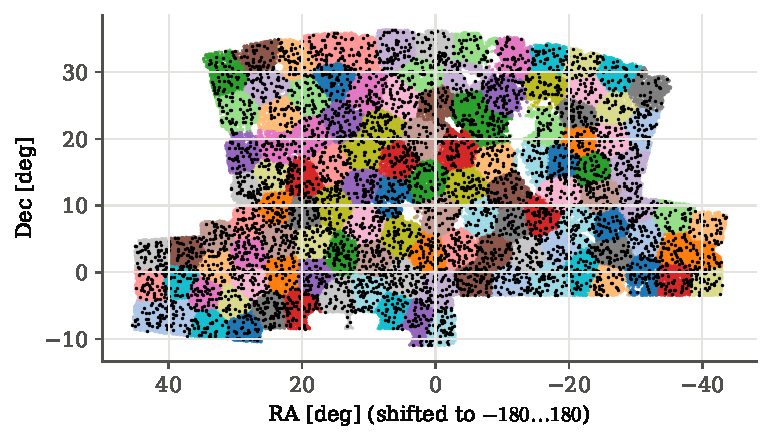
\includegraphics[width=0.95\linewidth]{figures/ch13/cmass_footprint.pdf}
\caption{The southern CMASS footprint. Coloured dots: a subsample of the randoms,
coloured by the jackknife region they belong to (\cref{13c:sec:jackknife}); black
dots: a subsample of the galaxies. The sky is seen from inside, so RA increases to
the left. The ragged edge and the small holes are the mask the randoms copy.}
\label{13c:fig:footprint}
\end{figure}

\begin{figure}[htbp]
\centering
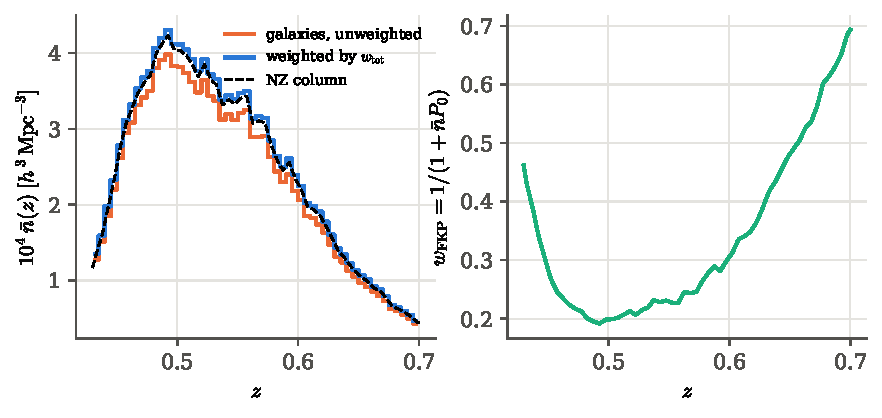
\includegraphics[width=0.95\linewidth]{figures/ch13/cmass_nz.pdf}
\caption{Left: the number density of CMASS South galaxies against redshift, counted
in shells of the fiducial cosmology, without weights (orange) and with the weight
$w_{\mathrm{tot}}$ of \cref{13c:sec:weights} (blue), and the catalogue's
\texttt{NZ} column (dashed), which matches the weighted histogram. Right: the FKP
weight each galaxy receives; it is lowest where the sample is densest.}
\label{13c:fig:nz}
\end{figure}

\paragraph{The code.}
\Cref{13c:fig:footprint,13c:fig:nz} show the result of
\pyname{code/ch13/21_cmass_catalogue.py}. The lines that matter are these.

\pyfile[firstline=56,lastline=78,firstnumber=56]{code/ch13/21_cmass_catalogue.py}{From angles and redshift to a position}

\pyname{comoving_distance_table} evaluates CAMB's $D_C(z)$ once on a fine grid and
multiplies by $h$ to work in $h^{-1}$Mpc; every galaxy's distance is then a linear
interpolation in that table, and \pyname{to_xyz} is \eqref{13c:eq:position}. The
script also reads the weights (\cref{13c:sec:weights}), keeps $\CmRanRatio$ randoms
per galaxy, and assigns each object to one of $\CmNjk$ patches of sky for the jackknife
(\cref{13c:sec:jackknife}).
\section{What the survey could not see: the weights}
\label{13c:sec:weights}

The random catalogue of \cref{13c:sec:files} knows how complete the survey was in
each patch of sky and how the density falls with redshift. It cannot know about
losses that depend on the galaxies themselves or on what the sky looked like on
the night the images were taken. A galaxy that sits right next to another one may
not get a fibre; a faint galaxy may not give a usable spectrum; a patch of sky
crowded with stars may yield fewer galaxy targets. None of these has anything to do
with cosmology, and all of them imprint a pattern on the galaxy counts that would be
read as clustering. The catalogue fixes them by attaching a \newterm{weight} to each
galaxy: a number that says how many galaxies this one stands for.

\paragraph{The principle behind every weight.}
The model of \cref{11a:sec:cox} is that the galaxies are a Poisson sample of the
density $\bar n(\bm x)[1+\delta_g(\bm x)]$, where $\bar n(\bm x)$ is the density the
survey would record if galaxies were not clustered. Suppose an effect that has
nothing to do with cosmology multiplies the probability of recording a galaxy at
$\bm x$ by a factor $f(\bm x)$, so the recorded galaxies are a Poisson sample of
$f\bar n(1+\delta_g)$. If each recorded galaxy is counted with weight $w=1/f$, the
expected weighted count in a small volume $\dd V$ is
\begin{align}
  \E\Bigl[\sum_{i\in\dd V}w_i\Bigr]
  &\eqby{1}\frac{1}{f(\bm x)}\;\E\bigl[N(\dd V)\bigr]
   \eqby{2}\frac{1}{f(\bm x)}\,f(\bm x)\,\bar n(\bm x)\bigl[1+\delta_g(\bm x)\bigr]\dd V
   =\bar n(\bm x)\bigl[1+\delta_g(\bm x)\bigr]\dd V .
  \label{13c:eq:weight-principle}
\end{align}
\begin{explain}
  \item All galaxies in the small volume share the same $f$, so the weight comes
        out of the sum, which is then the number $N(\dd V)$ of recorded galaxies.
  \item The mean of a Poisson count is its intensity times the volume
        (\cref{11a:eq:mean-count}).
\end{explain}
So the weighted galaxies are, on average, the galaxies a perfect survey would have
recorded. The inputs are physical ones we should state: the loss factor $f$ must
not depend on the cosmological field $\delta_g$ itself, and it must be known, or
measurable from something other than the galaxy clustering. Each weight below is
a way of estimating $1/f$ for one kind of loss, and each one bends one of these
inputs a little.

\subsection{Close pairs: the galaxy that did not get a fibre}
\label{13c:sec:wcp}

Two fibres cannot be plugged closer than $62''$ on one plate \srcref{Reid2016}{\S6.1}.
When two targets are closer than that and only one plate covers them, one of them
gets no spectrum. At $z=0.55$, $62''$ is a transverse distance
$D_C\theta=1427\times(62/206265)=0.43\,h^{-1}$Mpc. The lost galaxy is, more often than
not, a physical companion of the one that was observed: among close pairs where both
members did get redshifts (because two plates overlapped), $52\%$ belong to a
component concentrated within about $5\,h^{-1}$Mpc of each other along the line of
sight, and the rest are chance projections \srcref{Reid2016}{\S6.2, Fig.~10}. So the loss depends on the clustering itself,
and the random catalogue, which knows nothing about clustering, cannot reproduce it.

The catalogue's fix is to give the lost galaxy's weight to its nearest neighbour
with a good redshift: the column \texttt{WEIGHT\_CP} is $w_{\mathrm{cp}}=1$ plus the
number of collided targets a galaxy stands for (\cref{13c:fig:wcp}). This preserves
the number of galaxies in every region much larger than $0.4\,h^{-1}$Mpc: one galaxy
counted twice in place of two galaxies a few $h^{-1}$Mpc apart moves some pairs by a
few $h^{-1}$Mpc, which hardly matters in bins $8\,h^{-1}$Mpc wide at the acoustic
scale. Because the galaxy that got the fibre was chosen at random within the colliding
group, it is statistically equivalent to the one that did not, and the correction is
unbiased at transverse separations larger than the collision scale; below it, pairs
are missing, which we do not fit \srcref{Reid2016}{\S6.2}. In our
sample $\CmFracCp\%$ of the galaxies carry $w_{\mathrm{cp}}>1$, and they stand for
$\WtExtraCp$ collided targets in all.

\begin{figure}[htbp]
\centering
\begin{tikzpicture}[scale=1.0]
  \draw[faint,dashed] (1.6,1.2) circle (0.75);
  \fill[tangentgreen] (1.35,1.25) circle (2.4pt);
  \draw[bdryred,thick] (1.95,1.05) circle (2.4pt);
  \node[lbl,anchor=east] at (0.8,1.25) {observed};
  \node[lbl,anchor=west] at (2.45,0.95) {no fibre};
  \node[lbl] at (1.6,2.25) {$62''$ circle};
  \node[lbl] at (1.6,-0.35) {on the sky: two targets};
  \begin{scope}[xshift=5.6cm]
    \draw[faint,dashed] (1.6,1.2) circle (0.75);
    \fill[tangentgreen] (1.35,1.25) circle (3.6pt);
    \node[lbl,anchor=east] at (0.8,1.25) {$w_{\rm cp}=2$};
    \node[lbl] at (1.6,-0.35) {in the catalogue: one galaxy, weight 2};
  \end{scope}
  \draw[->,black!50,thick] (3.85,1.2) -- (4.85,1.2);
\end{tikzpicture}
\caption{Nearest-neighbour upweighting. Left: two targets closer than $62''$; only
one received a fibre. Right: the observed galaxy carries the missing one's weight.
Counts in any region much larger than the circle are unchanged on average.}
\label{13c:fig:wcp}
\end{figure}

\subsection{Redshift failures, stars and seeing}
\label{13c:sec:wsys}

\paragraph{Redshift failures.}
Some galaxies got a fibre but no reliable redshift, more often on fibres near the
edge of a plate and for galaxies that look fainter through the fibre
\cite{Ross2012,Reid2016}. Again the missing galaxy's
weight goes to its nearest neighbour with a good redshift, in the column
\texttt{WEIGHT\_NOZ}; a small refinement in DR12 moves weight towards fainter
neighbours, so the values are not exactly integers \srcref{Reid2016}{\S6.3}. In our
sample $\CmFracNoz\%$ of galaxies carry $w_{\mathrm{noz}}>1$, standing for $\WtExtraNoz$
failures.

\paragraph{Stars, and the reasoning that finds them.}
\emph{The event.} Ross et al.\ found that the number of CMASS targets per square
degree falls in parts of the sky where many stars are seen \cite{Ross2012}.
\emph{What could have produced it?} Two explanations are possible. Either the
regions near the Galactic plane, where stars are many, happen to hold fewer
galaxies, or stars interfere with finding galaxies. \emph{How likely is the observation
under each?} The galaxies are billions of light years away and the stars are in our
own Galaxy. Under the first explanation the galaxy density would know nothing about
the star density, and a steady trend with it across the whole survey would be a
coincidence. Under the second the trend is expected: a star close to a galaxy on the
sky hides it or spoils the measurement of its brightness and colours, on which the
selection cuts act. The trend is also stronger for galaxies of lower surface
brightness, the ones most easily spoiled, and only the second explanation predicts
that \cite{Ross2012}. So the
density is modelled as the true density times $A+B\,n_s$, a linear function of the
local star density $n_s$, with $A$ and $B$ fitted in bins of galaxy brightness
\srcref{Reid2016}{eq.~(45)}, and the weight is the inverse,
$w_{\mathrm{star}}=(A+Bn_s)^{-1}$: \eqref{13c:eq:weight-principle} with
$f=A+Bn_s$. A second weight $w_{\mathrm{see}}$ does the same for the blurring of the
images by the atmosphere, the seeing, and the catalogue stores their product,
$w_{\mathrm{systot}}=w_{\mathrm{star}}\,w_{\mathrm{see}}$ \srcref{Reid2016}{eq.~(49)}.
In our sample $95\%$ of the galaxies have $\CmSysLo<w_{\mathrm{systot}}<\CmSysHi$, with
mean $\WtMeanSys$. The correction is small per galaxy, but it varies smoothly over
tens of degrees, and on large scales that is exactly the kind of pattern that
masquerades as clustering: without it the stellar trend imprints an error larger
than the statistical one at $s>120\,h^{-1}$Mpc \cite{Ross2012}.

\subsection{Putting the weights together}
\label{13c:sec:wtot}

\paragraph{How many galaxies does one galaxy stand for?}
A galaxy with a good redshift stands for itself, plus the $w_{\mathrm{cp}}-1$
collided targets given to it, plus the $w_{\mathrm{noz}}-1$ failures given to it.
All of these stand-ins are at the same place on the sky, so the same star and seeing
correction applies to each. Therefore
\begin{align}
  w_{\mathrm{tot}}
  &\eqby{1}w_{\mathrm{systot}}\,\bigl[1+(w_{\mathrm{cp}}-1)+(w_{\mathrm{noz}}-1)\bigr]
  \eqby{2}w_{\mathrm{systot}}\,\bigl(w_{\mathrm{cp}}+w_{\mathrm{noz}}-1\bigr)
  \label{13c:eq:wtot}
\end{align}
\begin{explain}
  \item The count of galaxies this one represents, each corrected by the angular
        factor $1/f=w_{\mathrm{systot}}$ of \eqref{13c:eq:weight-principle}.
  \item Collect the ones.
\end{explain}
which is the total weight of the DR12 catalogues \srcref{Reid2016}{eq.~(50)},
\srcref{Ross2012}{eq.~(25)}. Writing the sum minus one, rather than the product
$w_{\mathrm{cp}}w_{\mathrm{noz}}$, says that a collided target and a failed
redshift are two different missing galaxies, not one galaxy missing twice.

\paragraph{Example: the books balance.}
Summed over our $\CmNgal$ galaxies, $\sum(w_{\mathrm{cp}}+w_{\mathrm{noz}}-1)=\WtSumStand$:
the galaxies with redshifts plus the $\WtExtraCp$ collided targets and the
$\WtExtraNoz$ failures that they stand for. With the angular weights the total is
$\sum w_{\mathrm{tot}}=\CmSumWtot$, about $1\%$ more, the mean of $w_{\mathrm{systot}}$.
\Cref{13c:fig:nz} shows the redshift distribution before and after weighting; the
weighted histogram is the one the randoms copy, and it matches the catalogue's
\texttt{NZ} column.

\paragraph{The FKP weight is a choice, not a correction.}
The weights so far undo losses. The last one decides how much each part of the
survey should count. In \cref{11a:sec:fkp-weight} we derived that the variance of
the measured clustering at wavenumber $k$ is smallest when each region is weighted by
$w=1/(1+\bar nP)$, where $P$ is the power at that $k$ (\cref{11a:eq:fkp-weight}). A
sparse region is noisy, because its fluctuations are mostly shot noise, so it gets
weight near $1$; a dense region is limited by sample variance, so piling up more of
its galaxies helps little, and each of them is down-weighted. The catalogue uses
$P_0=10^4\,h^{-3}\mathrm{Mpc}^3$, the observed power near $k\approx0.15\,h\,
\mathrm{Mpc}^{-1}$ \srcref{Reid2016}{eq.~(53)}, so
$w_{\mathrm{FKP}}=1/(1+\bar n(z)\,10^4)$. Recomputing it from the \texttt{NZ}
column reproduces the stored values to $\CmFkpMaxDiff$. Across our sample it runs from
$\CmFkpLo$ at the density peak to $\CmFkpHi$ at the far edge (\cref{13c:fig:nz},
right).

\paragraph{Why the randoms carry the FKP weight but not $w_{\mathrm{tot}}$.}
The randoms already follow $\bar n(\bm x)$, the density of a complete survey: their
angular density follows the completeness and their redshifts follow the weighted
galaxies. The galaxies needed $w_{\mathrm{tot}}$ to be brought to that same density.
The FKP weight is different: it multiplies the field we analyse, galaxies minus
randoms (\cref{11a:eq:fkp-field}), and both terms must be multiplied by the same
function of position, or the weighted field would not average to zero where there is
no clustering. So the final weights are \srcref{Reid2016}{\S6.7}
\begin{equation}
  w_i^{\mathrm{gal}}=w_{\mathrm{tot},i}\,w_{\mathrm{FKP},i},\qquad
  w_j^{\mathrm{ran}}=w_{\mathrm{FKP},j}.
  \label{13c:eq:final-weights}
\end{equation}

\paragraph{Example: one galaxy's weight.}
A galaxy at $z=0.50$, where $\bar n=4.2\times10^{-4}\,h^3\mathrm{Mpc}^{-3}$, that
received the weight of one collided neighbour ($w_{\mathrm{cp}}=2$, $w_{\mathrm{noz}}=1$)
in a slightly star-crowded field ($w_{\mathrm{systot}}=1.05$) has
$w_{\mathrm{tot}}=1.05\times(2+1-1)=2.10$ and $w_{\mathrm{FKP}}=1/(1+4.2)=0.19$, so it
enters the pair counts with weight $0.40$. An isolated galaxy at $z=0.68$, where
$\bar n=0.7\times10^{-4}$, has $w_{\mathrm{tot}}\approx1$ and $w_{\mathrm{FKP}}=0.59$: it
counts for half again as much as the first, although the first stands for two galaxies.

\subsection{Weighted pair counts, and why they still estimate \texorpdfstring{$\xi$}{xi}}
\label{13c:sec:weighted-counts}

With weights, the normalised counts of \cref{11a:eq:dd-dr-rr} become weighted sums,
each divided by the total weight of all possible pairs of its kind:
\begin{equation}
  DD(s)=\frac{\sum_{i\neq j}w_iw_j\,[s_{ij}\in\text{bin}]}{\bigl(\sum_iw_i\bigr)^2-\sum_iw_i^2},
  \quad
  DR(s)=\frac{\sum_{i,j}w_iw_j'\,[s_{ij}\in\text{bin}]}{\sum_iw_i\sum_jw_j'},
  \label{13c:eq:weighted-counts}
\end{equation}
and $RR$ like $DD$ with the random weights $w'$. Here $[\,\cdot\,]$ is $1$ if the pair's
separation falls in the bin and $0$ otherwise, and the sums run over ordered pairs.
The denominator of $DD$ is $\sum_{i\ne j}w_iw_j$, the weight of all ordered pairs
with $i\ne j$: the square of the sum contains every product $w_iw_j$ once for each
order, including $i=j$, and subtracting $\sum w_i^2$ removes those.

\emph{Why the ratio still measures $1+\xi$.} Take the galaxies as a Poisson sample of
intensity $\lambda(\bm x)=f\bar n(1+\delta_g)$, each carrying the weight $w(\bm x)$ of
\eqref{13c:eq:final-weights}, so that $w\lambda=w_{\mathrm{FKP}}\bar n(1+\delta_g)$ on
average by \eqref{13c:eq:weight-principle}. Write $u(\bm x)\equiv
w_{\mathrm{FKP}}(\bm x)\bar n(\bm x)$ for this weighted mean density. For distinct
points of a Cox process the density of pairs at $\bm x_1,\bm x_2$ is
$\bar n_1\bar n_2[1+\xi(s)]$ (\cref{11a:eq:pair-prob}), so
\begin{align}
  \E\Bigl[\sum_{i\ne j}w_iw_j[s_{ij}\in\text{bin}]\Bigr]
  &\eqby{1}\int\!\!\int u(\bm x_1)\,u(\bm x_2)\,\bigl[1+\xi(s_{12})\bigr]
     [s_{12}\in\text{bin}]\,\dd V_1\dd V_2\nonumber\\
  &\eqby{2}\bigl[1+\bar\xi_{\mathrm{bin}}\bigr]
     \int\!\!\int u(\bm x_1)\,u(\bm x_2)\,[s_{12}\in\text{bin}]\,\dd V_1\dd V_2 .
  \label{13c:eq:weighted-dd}
\end{align}
\begin{explain}
  \item The pair density times the two weights, integrated over all positions; the
        weight times the recorded density is $u$, by \eqref{13c:eq:weight-principle}.
  \item In a bin narrow enough that $\xi$ hardly changes across it, $1+\xi$ comes out
        as its value $1+\bar\xi_{\mathrm{bin}}$ in the bin.
\end{explain}
The random catalogue has intensity proportional to $\bar n$ and weights
$w_{\mathrm{FKP}}$, so its weighted pair count is the same integral without the
factor $1+\bar\xi$, multiplied by a constant that the normalisations remove. The
two survey integrals cancel in the ratio, and $DD/RR\to1+\bar\xi_{\mathrm{bin}}$; the
Landy--Szalay combination of \cref{11a:sec:xi-estimators} inherits the same
property, with its reduced sensitivity to the edges. The derivation also shows what
can go wrong: if the galaxies' weighted density $w\lambda$ and the randoms'
weighted density differ in shape, through a systematic not captured by a weight,
the cancellation fails and the difference is read as clustering.

\begin{figure}[htbp]
\centering
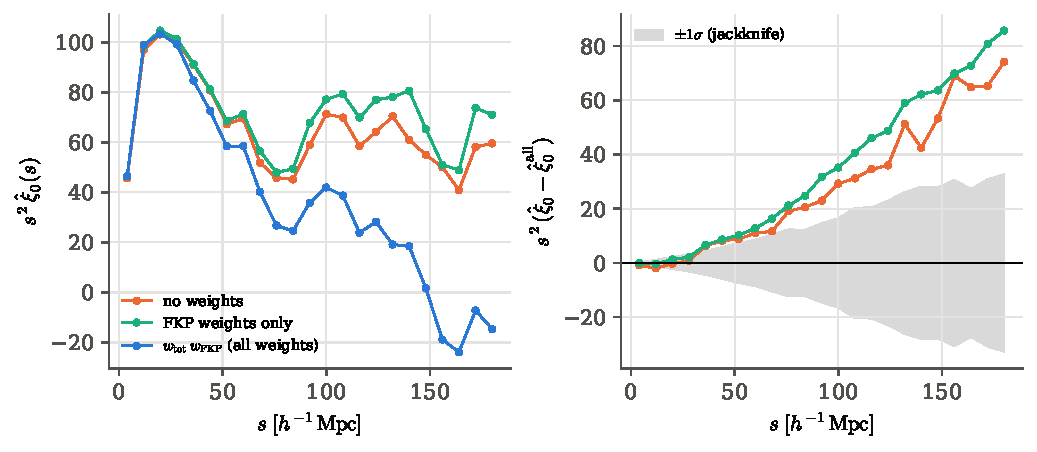
\includegraphics[width=0.95\linewidth]{figures/ch13/cmass_weights.pdf}
\caption{What the weights do to the measured monopole. Left: $s^2\hat\xi_0$ with no
weights, with FKP weights only, and with all weights. Right: the difference from the
fully weighted measurement, against the jackknife error band of
\cref{13c:sec:jackknife}. Without $w_{\rm tot}$ the clustering beyond
$35\,h^{-1}$Mpc is too high, by more than one error bar over most of that range and by
about two at the largest separations.}
\label{13c:fig:weights}
\end{figure}

\Cref{13c:fig:weights} shows the measurement of \cref{13c:sec:paircounts} with three
choices of weights. Below $30\,h^{-1}$Mpc the three agree to a few per cent. In the first bin, which holds
$\xi$ at $4\,h^{-1}$Mpc, the unweighted value is $1.8\%$ lower, and with the small
jackknife error there that is a $2\sigma$ difference; the FKP-only measurement
reproduces the fully weighted value to a tenth of an error bar. So at small scales it
is the redistribution of weight by the FKP factor, not the corrections for the lost
galaxies, that matters, and the lost companions of \cref{13c:sec:wcp}, a few per cent
of the galaxies, move $\xi$ at $4\,h^{-1}$Mpc by much less than its error. The large scales are where the weights act. Without $w_{\rm tot}$ the
monopole lies above the weighted one at every separation beyond $35\,h^{-1}$Mpc. The
shift is nearly the same in $\xi$ at all of these separations, about $0.003$, which
is $1$--$1.5$ jackknife errors at $40$--$70\,h^{-1}$Mpc and about two errors at
$150$--$180\,h^{-1}$Mpc, where the error bars are smaller (the right panel multiplies
both by $s^2$). A nearly constant offset is not a feature at one scale but a change in the
mean density that the pairs are measured against. That is the signature Ross et al.\ traced to the
density of foreground stars \cite{Ross2012}: where stars are dense, fewer galaxies
are targeted, and since the stellar density varies smoothly over tens of degrees, the
missing galaxies imprint a pattern on very large scales that pair counts read as extra
clustering. The weight $w_{\rm star}$ removes the pattern, as
\eqref{13c:eq:weight-principle} says it should. Beyond $35\,h^{-1}$Mpc the FKP weight alone moves the monopole by at most two-thirds
of an error bar, since it only reweights galaxies by redshift. In all three versions the bump near
$100\,h^{-1}$Mpc is present; what differs is the smooth shape it sits on, which the
broad-band terms of the fit in \cref{13c:sec:reproduce} are designed to absorb. Without
the corrective weights the broad band would be wrong by more than the statistical error,
and any analysis of the full shape of $\xi$, rather than only of the peak position,
would be biased.
\section{Counting pairs: the correlation function of CMASS South}
\label{13c:sec:paircounts}

We now have $\CmNgal$ weighted galaxies and, for the counts, $\XiNran$ randoms
($\XiRandRatio$ per galaxy) at known positions. The Landy--Szalay estimator of
\cref{11a:sec:xi-estimators},
\begin{equation}
  \hat\xi_0(s)=\frac{DD(s)-2DR(s)+RR(s)}{RR(s)},
  \label{13c:eq:ls}
\end{equation}
with the weighted, normalised counts of \eqref{13c:eq:weighted-counts}, asks for
three numbers in each separation bin. The subscript $0$ says that pairs are counted
in every direction, so the result is the angle average, the monopole, of the
redshift-space correlation function. The difficulty is only the number of pairs:
the randoms alone form $10^{12}$ ordered pairs, and a double loop that
computes each distance would take days.

\subsection{How a tree counts pairs without visiting them}
\label{13c:sec:tree}

A $k$-d tree sorts the points into nested boxes: the whole set is split in half
along its longest side, each half again, and so on, until each box holds a few dozen
points. For each box the tree stores its corners and the total weight of its points.
To count the pairs between two boxes in our bins, \pyname{cKDTree.count_neighbors}
looks first at the smallest and the largest distance that any point in one box can
have from any point in the other, which follow from the corners alone.
\begin{itemize}[itemsep=1pt,leftmargin=1.2em]
  \item If both lie inside the same bin, every pair between the two boxes is in that
        bin, and the product of the two total weights is added at once.
  \item If both lie beyond the last bin edge, no pair counts, and the boxes are
        skipped.
  \item Otherwise the boxes are split and their children are compared.
\end{itemize}
\emph{Example.} Two boxes of side $10\,h^{-1}$Mpc whose centres are $100\,h^{-1}$Mpc
apart contain pairs from $100-17$ to $100+17\,h^{-1}$Mpc (the diagonal of a cube of
side $10$ is $17$), which spans five of our $8\,h^{-1}$Mpc bins; they must be opened.
Two boxes of side $2\,h^{-1}$Mpc at the same distance span at most $3.5\,h^{-1}$Mpc,
and most such pairs of boxes fall inside one bin. The work is therefore spent on box
pairs that straddle a bin edge, a small fraction of all pairs, and the counts are
exact. (The script of \cref{11a:sec:xi-python} used the same routine in two
dimensions.) The cost still grows with the number of pairs inside the largest
separation, which is why we stop at $184\,h^{-1}$Mpc and use $\XiRandRatio$ randoms
per galaxy rather than the fifty of the BOSS analyses \cite{Cuesta2016}. The random
catalogue's own counting noise shrinks as the number of randoms grows; at five per
galaxy it is a small addition to the counting noise of the galaxies, which is itself
smaller than the sample variance at the acoustic scale for a sample with $\bar nP$
between $1$ and $4$ (\cref{13c:sec:positions}).

\subsection{Counts for the jackknife at no extra cost}
\label{13c:sec:leave-one-out}

\Cref{13c:sec:jackknife} will need the correlation function recomputed $\CmNjk$
times, each time with one patch of sky left out. Recounting all pairs each time
would multiply the cost by $\CmNjk$. It is not necessary, because a pair count is a
sum over pairs, and a sum can be split by where the pairs live.

Divide the footprint into regions $k=1,\dots,\CmNjk$ (the colours of
\cref{13c:fig:footprint}). For two sets of points $A$ and $B$ write $C(A,B)$ for the
weighted count of ordered pairs with the first member in $A$ and the second in $B$,
in a given bin, and let $D$ be all galaxies, $D_k$ those in region $k$, and
$R$, $R_k$ the same for the randoms. Leaving region $k$ out removes every pair with
at least one member in $D_k$. Those are the pairs whose first member is in $D_k$, plus
those whose second member is in $D_k$, minus the pairs counted twice, which have both
members in $D_k$:
\begin{align}
  DD_{-k}
  &\eqby{1}C(D,D)-\bigl[C(D_k,D)+C(D,D_k)-C(D_k,D_k)\bigr]\nonumber\\
  &\eqby{2}C(D,D)-2\,C(D_k,D)+C(D_k,D_k),
  \label{13c:eq:dd-minus-k}\\
  DR_{-k}
  &\eqby{3}C(D,R)-C(D_k,R)-C(D,R_k)+C(D_k,R_k),
  \label{13c:eq:dr-minus-k}
\end{align}
and $RR_{-k}$ like $DD_{-k}$ with $R$ in place of $D$.
\begin{explain}
  \item The number of elements in a union of two sets is the sum of their numbers
        minus the number in their intersection (inclusion--exclusion).
  \item A distance does not care about the order of the pair, so
        $C(D,D_k)=C(D_k,D)$.
  \item For galaxy--random pairs the two members are of different kinds: remove
        pairs whose galaxy is in region $k$ and pairs whose random is in region $k$,
        and add back the pairs where both are.
\end{explain}
So for each region we compute five counts, $C(D_k,D)$, $C(D_k,D_k)$, $C(D_k,R)$,
$C(D,R_k)$, $C(D_k,R_k)$, and two more for the randoms, $C(R_k,R)$ and $C(R_k,R_k)$.
Summing $C(D_k,D)$ over $k$ gives the full count $C(D,D)$, so the full measurement
is a by-product, and the total work is about that of one full count. The
normalisations of \eqref{13c:eq:weighted-counts} are recomputed for each
leave-one-out sample from the sums of the weights outside region $k$.

\begin{figure}[htbp]
\centering
\begin{tikzpicture}[scale=0.95]
  \draw[faint] (0,0) rectangle (4.2,2.6);
  \fill[formblue!14] (2.8,0) rectangle (4.2,2.6);
  \draw[faint] (2.8,0) -- (2.8,2.6);
  \node[lbl] at (3.5,2.85) {region $k$};
  \node[lbl] at (1.4,2.85) {the rest};
  \foreach \x/\y in {0.5/0.6,1.1/1.9,1.9/1.1,2.3/2.2,3.2/0.7,3.7/1.8,3.5/1.2}{
    \fill[black!70] (\x,\y) circle (1.6pt);}
  \draw[tangentgreen,thick] (0.5,0.6) -- (1.9,1.1);
  \draw[fibreorange,thick] (2.3,2.2) -- (3.7,1.8);
  \draw[bdryred,thick] (3.2,0.7) -- (3.5,1.2);
  \draw[tangentgreen,thick] (5.0,2.1) -- (5.6,2.1);
  \node[lbl,anchor=west] at (5.7,2.1) {both outside $k$: kept};
  \draw[fibreorange,thick] (5.0,1.4) -- (5.6,1.4);
  \node[lbl,anchor=west] at (5.7,1.4) {one in $k$: removed, counted in $C(D_k,D)$};
  \draw[bdryred,thick] (5.0,0.7) -- (5.6,0.7);
  \node[lbl,anchor=west] at (5.7,0.7) {both in $k$: removed, counted twice in $2C(D_k,D)$,};
  \node[lbl,anchor=west] at (5.7,0.3) {so added back once with $C(D_k,D_k)$};
\end{tikzpicture}
\caption{Leaving one region out of a pair count. A pair with one member in region $k$
appears once, in $C(D_k,D)$ or in $C(D,D_k)$ according to its order. A pair with both
members in $k$ appears in both of those, so subtracting $2C(D_k,D)$ removes it twice,
and $C(D_k,D_k)$ restores one copy.}
\label{13c:fig:inclusion}
\end{figure}

\subsection{The code, and what it measured}
\label{13c:sec:xi-python}

\pyfile[firstline=48,lastline=72,firstnumber=48]{code/ch13/22_cmass_xi.py}{Region-by-region pair counts and the Landy--Szalay estimator}

\pyname{pairs} calls the tree with the bin edges $0,8,\dots,184\,h^{-1}$Mpc and the
weights of both sets, and drops the first entry, which holds the pairs at zero
distance: a point paired with itself. \pyname{region_counts} builds small trees for
the galaxies and randoms of one region and counts them against the full trees, the
five plus two counts listed above. \pyname{landy_szalay} is \eqref{13c:eq:ls} with
the normalisations of \eqref{13c:eq:weighted-counts}. The regions are independent of
each other, so the script farms them out to $\XiNproc$ processes; the fully weighted
measurement took $\XiTime$\,s.

\begin{figure}[htbp]
\centering
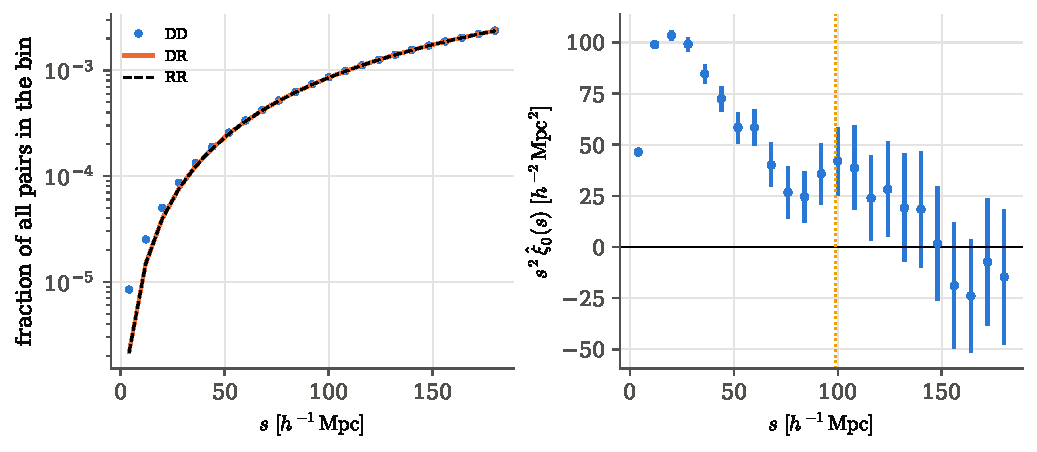
\includegraphics[width=0.95\linewidth]{figures/ch13/cmass_counts.pdf}
\caption{Left: the three weighted, normalised pair counts. Beyond $50\,h^{-1}$Mpc
they differ by a few per cent at most, too little to see on a logarithmic axis; the
correlation function lives in these small differences. Right: the Landy--Szalay
monopole times $s^2$, with jackknife error bars (\cref{13c:sec:jackknife}). The
dotted line marks the fiducial sound horizon, $r_dh=\CmRdH\,h^{-1}$Mpc.}
\label{13c:fig:counts}
\end{figure}

\Cref{13c:fig:counts} is the measurement. The three counts on the left follow the
geometry of the survey: they rise as $s^2$, since a shell of radius $s$ holds a
volume growing as $s^2$, and grow more slowly once the shell starts to leave the survey.
Only at small separations does $DD$ visibly exceed $RR$; beyond $50\,h^{-1}$Mpc they
agree to a few per cent, and the correlation function is that small excess. On the right, multiplying by $s^2$ makes the slow
decay of $\xi_0$ visible on a linear axis, and a modest bump rises above the declining trend near
$100\,h^{-1}$Mpc, close to the fiducial ruler $r_dh$. At $s=100\,h^{-1}$Mpc we measure
$\hat\xi_0=(\XiAtHundred\pm\XiErrHundred)\times10^{-3}$: a one-part-in-two-hundred
excess of pairs, read off from $\XiPairsDD$ ordered galaxy pairs closer than $184\,h^{-1}$Mpc. Whether the bump
is the acoustic peak or a fluctuation is a question for an error bar and a fit.
\section{Error bars from the data alone: the jackknife}
\label{13c:sec:jackknife}

In the mock surveys of \cref{11a:sec:bao-mocks} the covariance of $\hat\xi$ came from
fifteen hundred simulated boxes. The BOSS analyses did the same with about a
thousand simulated copies of the real survey, each with its footprint, its density
and its redshift distribution \cite{Cuesta2016,Alam2017}. Producing those copies is a
research project in itself. We have one sky. The question an error bar answers is:
if we could observe another patch of the Universe with the same shape and the same
galaxies, how different would $\hat\xi_0$ be? We cannot observe another patch. But
the survey is made of many smaller patches, and how much the answer moves when one
of them is left out tells us how much it depends on which galaxies we happened to
observe. That is the idea of the \newterm{jackknife}, a cousin of the bootstrap of
\cref{3b:sec:bootstrap} and of the leave-one-group-out error of
\cref{11b:sec:void-ap}.

\subsection{The simplest case first: the mean of \texorpdfstring{$N$}{N} numbers}
\label{13c:sec:jk-mean}

Take $N$ independent measurements $x_1,\dots,x_N$ with a common variance $\sigma^2$,
and the estimate $\bar x$. Its variance is $\sigma^2/N$, estimated by $s^2/N$ with
$s^2=\sum_k(x_k-\bar x)^2/(N-1)$. The jackknife reaches the same number without
knowing that the estimate is a mean. Leave out measurement $k$ and recompute:
$\bar x_{-k}=(N\bar x-x_k)/(N-1)$. The average of these $N$ leave-one-out values is
$\bar x$ itself, because each $x_j$ is left out exactly once. How far does each
leave-one-out value sit from it?
\begin{align}
  \bar x_{-k}-\bar x
  &\eqby{1}\frac{N\bar x-x_k-(N-1)\bar x}{N-1}
   =\frac{\bar x-x_k}{N-1},
  \nonumber\\
  \frac{N-1}{N}\sum_{k=1}^N\bigl(\bar x_{-k}-\bar x\bigr)^2
  &\eqby{2}\frac{N-1}{N}\,\frac{1}{(N-1)^2}\sum_{k=1}^N(x_k-\bar x)^2
   \eqby{3}\frac{1}{N}\,\frac{\sum_k(x_k-\bar x)^2}{N-1}
   =\frac{s^2}{N}.
  \label{13c:eq:jk-mean}
\end{align}
\begin{explain}
  \item Put both terms over the common denominator $N-1$.
  \item Square the first line and sum over $k$.
  \item Cancel one factor of $N-1$.
\end{explain}
So the jackknife variance, $\frac{N-1}{N}\sum_k(\bar x_{-k}-\bar x)^2$, is exactly the
usual estimate of the variance of a mean. The prefactor is the surprising part.
For $N$ independent repetitions we would divide by $N-1$; here we multiply by $N-1$.
The leave-one-out values are far closer to each other than independent repetitions
would be, because any two of them share $N-2$ of their $N-1$ measurements: each
deviation is the deviation of one measurement shrunk by $1/(N-1)$, and the prefactor
undoes that shrinkage.

\paragraph{Example: three numbers.}
For $x=(1,2,6)$, $\bar x=3$ and $s^2=(4+1+9)/2=7$, so $s^2/N=2.33$. Leaving one out
gives $4$, $3.5$, $1.5$, which average to $3$ with deviations $1$, $0.5$, $-1.5$; the
jackknife gives $\frac23(1+0.25+2.25)=2.33$. The same number, from a recipe that only
needed to recompute the estimate.

\begin{workdef}[jackknife covariance]
Split the data into $N$ subsets \unpack{here, $\CmNjk$ patches of sky of similar
area}. Recompute the estimate with subset $k$ removed, giving the vector
$\hat{\bm\xi}_{-k}$ \unpack{the binned correlation function without patch $k$}, for
each $k$, and let $\bar{\bm\xi}$ be their average. Then
\begin{equation}
  \hat\Cmat_{\mathrm{JK}}=\frac{N-1}{N}\sum_{k=1}^N
  \bigl(\hat{\bm\xi}_{-k}-\bar{\bm\xi}\bigr)\bigl(\hat{\bm\xi}_{-k}-\bar{\bm\xi}\bigr)\T .
  \label{13c:eq:jk-cov}
\end{equation}
\emph{Operationally:} \cref{13c:sec:leave-one-out} gives every
$\hat{\bm\xi}_{-k}$ from region-by-region pair counts at the cost of one
measurement.
\end{workdef}

The off-diagonal elements come for free: if leaving out a patch raises $\hat\xi$ in
one bin, it usually raises it in the neighbouring bins too, because the same pairs
and the same structures contribute to both, and \eqref{13c:eq:jk-cov} records that
co-movement as a covariance.

\subsection{What the jackknife gets wrong}
\label{13c:sec:jk-bias}

For a mean, \eqref{13c:eq:jk-mean} is exact. For any other statistic of independent
data, Efron and Stein proved that the jackknife variance is biased upward in
expectation: on average it is too large, never too small \cite{EfronStein1981}. The smallest
example is the square of a mean, $\hat\theta=\bar x^2$, for $N$ Gaussian measurements
of mean $\mu$ and variance $\sigma^2$. Its true variance is that of the square of a
Gaussian variable of mean $\mu$ and variance $\sigma^2/N$, namely
$4\mu^2\sigma^2/N+2\sigma^4/N^2$. With $d_k=\bar x_{-k}-\bar x=(\bar x-x_k)/(N-1)$
from \eqref{13c:eq:jk-mean},
\begin{align}
  \hat\theta_{-k}-\hat\theta
  &\eqby{1}(\bar x+d_k)^2-\bar x^2=d_k\,(2\bar x+d_k),
  \nonumber\\
  \frac{N-1}{N}\sum_k\bigl(\hat\theta_{-k}-\hat\theta\bigr)^2
  &\eqby{2}\frac{N-1}{N}\Bigl[4\bar x^2\sum_kd_k^2+4\bar x\sum_kd_k^3+\sum_kd_k^4\Bigr]
   \eqby{3}\frac{4\bar x^2s^2}{N}+O(N^{-3}),
  \nonumber\\
  \E\Bigl[\frac{4\bar x^2s^2}{N}\Bigr]
  &\eqby{4}\frac{4}{N}\Bigl(\mu^2+\frac{\sigma^2}{N}\Bigr)\sigma^2
   =\frac{4\mu^2\sigma^2}{N}+\frac{4\sigma^4}{N^2}.
  \label{13c:eq:jk-bias}
\end{align}
\begin{explain}
  \item Square out the bracket.
  \item Square the first line and sum. The sum is centred on $\hat\theta$ rather than
        on the average of the leave-one-out values, which differs from it by
        $O(N^{-2})$ and changes the result only at order $N^{-3}$.
  \item $\sum_kd_k^2=s^2/(N-1)$ by \eqref{13c:eq:jk-mean}. For a Gaussian sample
        $\bar x$ is independent of the deviations $x_k-\bar x$, so $\sum_kd_k^3$, odd in
        them, averages to zero, and $\sum_kd_k^4\sim3\sigma^4/N^3$.
  \item $\E[\bar x^2]=\mu^2+\sigma^2/N$, because $\bar x$ has mean $\mu$ and variance
        $\sigma^2/N$, and $\E[s^2]=\sigma^2$.
\end{explain}
The first term of the jackknife variance is the standard error-propagation result
$(2\mu)^2\sigma^2/N$, and its next term, $4\sigma^4/N^2$, is twice the
$2\sigma^4/N^2$ of the true variance. The jackknife is too large, here by a second-order amount that fades
as $N$ grows, in line with the theorem. A
correlation function from patches of sky bends the inputs of that result in three
ways.
\begin{itemize}[itemsep=1pt,leftmargin=1.2em]
  \item \emph{The patches are not independent.} Neighbouring patches share large
        structures, and a fluctuation larger than a patch moves several of them
        together; the leave-one-out values then move together too, and that part
        of the variance is under-represented. Fluctuations on scales larger than
        the whole survey are invisible to any internal method.
  \item \emph{Pairs straddle the boundaries.} Removing a patch removes the pairs
        between it and its neighbours as well. Our patches are about $21\,\mathrm{deg}^2$,
        some $120\,h^{-1}$Mpc across on the sky at the sample's distance, so at the
        acoustic scale most of the pairs that a patch removes cross its boundary.
  \item \emph{The patches are unequal.} Ours hold between $\CmJkMin$ and $\CmJkMax$
        galaxies, while the derivation assumed exchangeable pieces.
\end{itemize}
Norberg et al.\ compared jackknife errors with the scatter of many simulated surveys
\cite{Norberg2009}. The jackknife returned the right variance on large scales and too
large a variance on small scales, and its errors were noisy enough that an interval
quoted as $2\sigma$ from it could correspond to anything from $1\sigma$ to $3\sigma$.
We should therefore read our error bars as good to some tens of per cent, which is
the price of not having mocks.

\paragraph{Inverting a noisy matrix.}
The fit of \cref{13c:sec:reproduce} needs $\hat\Cmat^{-1}$, and the inverse of a noisy
covariance estimate is biased high: noise makes some directions look better measured
than they are. For a covariance from $N$ independent Gaussian samples and $n_b$ bins,
multiplying the inverse by $(N-n_b-2)/(N-1)$ removes the bias
(\cref{8b:sec:hartlap}). With $N=\CmNjk$ jackknife samples and the $n_b=\BaoNbFit$ bins
of the fit this factor is $\BaoHart$. Jackknife samples are not independent draws,
so the factor is only a guide; it is the reason for using many regions.

\subsection{A check against the published mocks}
\label{13c:sec:jk-check}

There is one test we can make. Cuesta et al.\ published the CMASS monopole of the
whole sample, north and south, with error bars from 956 simulated surveys
\cite{Cuesta2016}. How should our errors compare with theirs? The variance of a
clustering measurement comes from the finite number of independent Fourier modes in
the volume, and that number is proportional to the volume (the mode count of
\cref{11a:sec:bao-fisher}). At the same redshifts and density the error therefore
scales as $V^{-1/2}$, so a sample with $3.71$ times our area should have errors
$\sqrt{9376/2525}=\AreaScale$ times smaller.

\begin{figure}[htbp]
\centering
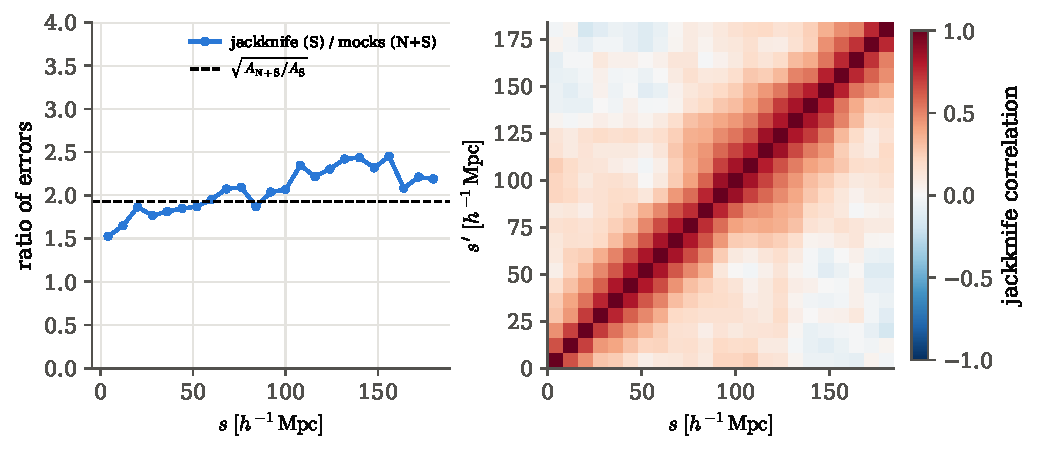
\includegraphics[width=0.95\linewidth]{figures/ch13/cmass_errors.pdf}
\caption{Left: our jackknife error on $\hat\xi_0$ (south only) divided by the mock
error of the published north-plus-south measurement, bin by bin; the dashed line is
the ratio $\sqrt{A_{\rm N+S}/A_{\rm S}}$ expected from the areas alone. Right: the
correlation matrix of our jackknife covariance; neighbouring bins are strongly
correlated, as they share pairs and structures.}
\label{13c:fig:errors}
\end{figure}

\Cref{13c:fig:errors} shows the comparison. Over the fitted range $30<s<180\,h^{-1}$Mpc
the median ratio is $\ErrRatio$, against $\AreaScale$ expected from the areas: our
jackknife errors are $\ErrRatioOverArea$ times what scaling the mock errors would
give. That is within the tens of per cent expected of a jackknife, and since the
two error bars come from entirely different routes, one from the data alone and one
from a thousand simulations, it is a real test of both. The right panel shows that
neighbouring bins are strongly correlated. A fit that used only the diagonal errors
would count the same information several times, which is why the fit uses the full
matrix.

\begin{figure}[htbp]
\centering
\begin{tikzpicture}[scale=0.9]
  \foreach \k/\lab in {0/1,1/2,2/3,3/4}{
    \begin{scope}[xshift=\k*3.3cm]
      \foreach \i in {0,1,2}{\foreach \j in {0,1}{
        \draw[faint,fill=formblue!10] (\i*0.8,\j*0.8) rectangle ++(0.8,0.8);}}
      \pgfmathtruncatemacro{\ii}{mod(\k,3)}
      \pgfmathtruncatemacro{\jj}{\k>2 ? 1 : 0}
      \fill[white] (\ii*0.8,\jj*0.8) rectangle ++(0.8,0.8);
      \draw[bdryred,thick] (\ii*0.8,\jj*0.8) rectangle ++(0.8,0.8);
      \node[lbl] at (1.2,-0.35) {$\hat{\bm\xi}_{-\lab}$};
    \end{scope}}
  \node[lbl] at (13.4,0.8) {$\cdots$};
\end{tikzpicture}
\caption{The jackknife in pictures: the footprint (six patches drawn here; $\CmNjk$ in
the analysis) is measured again and again, each time with one patch removed (red).
The spread of the leave-one-out results, multiplied by $(N-1)/N$, is the covariance.}
\label{13c:fig:jk-cartoon}
\end{figure}
\section{The acoustic peak of CMASS South, and the BOSS distance}
\label{13c:sec:reproduce}

The ratio $D_V(z)/r_d$ has appeared twice before. In \cref{11a:sec:alpha} we saw why a
galaxy survey measures it: the acoustic shell has a comoving radius $r_d$ fixed in the
early Universe, and the survey sees that shell at a size set by the distance to the
galaxies, so only the ratio of the two is observed. In \cref{11a:sec:bao-desi} we set
the published DESI values of $D_V/r_d$ beside the prediction of the Planck 2018 model
and found them within one or two standard deviations of it, with errors of one to two
per cent. Those were numbers someone else had measured. Now the same ratio comes out
of our own pipeline, at the redshift $z_{\rm eff}=\BaoZeff$ of the CMASS galaxies,
from the correlation function $\hat\xi_0(s)$ of \cref{13c:sec:paircounts} and the
jackknife covariance of \cref{13c:sec:jackknife}. What is new is that nothing has been
done for us: the coordinates, the weights, the pair counts and the error bars are all
ours, and the comparison is with collaborations that measured the same galaxies.

\subsection{Their question}
\label{13c:sec:repro-question}

When BOSS released its ninth data set in 2012, the acoustic peak had been seen in
galaxy surveys for seven years, but never with enough galaxies to measure its position
to better than a few per cent. Anderson et al.\ asked whether the first $264{,}283$
CMASS galaxies could detect the peak beyond reasonable doubt and turn it into a
distance at $z=0.57$ precise to two per cent \cite{Anderson2012}. They found the peak
at about $5\sigma$ and $D_V(0.57)/r_s=13.67\pm0.22$, a $1.7\%$ distance
\srcref{Anderson2012}{abstract, Table~2}. Four years later the survey was complete.
Cuesta et al.\ repeated the measurement on all $777{,}202$ CMASS galaxies of the final
release \cite{Cuesta2016}, and Alam et al.\ combined it with the other BOSS analyses
into the collaboration's final distances at three redshifts \cite{Alam2017}.

Our question is narrower. With $27\%$ of the final sample (the southern cap,
\cref{13c:tab:boss}) and with error bars from the data alone, do we see the same peak,
how strongly, and do we get a distance consistent with theirs?

\subsection{Their setup, in plain terms}
\label{13c:sec:repro-setup}

Every BAO analysis makes the same four choices, and the numbers in
\cref{13c:tab:setup} are those choices for the three analyses we compare.

\emph{A fiducial cosmology.} To turn $(\mathrm{RA},\mathrm{Dec},z)$ into positions one
needs a distance--redshift relation (\cref{13c:sec:positions}), so each analysis
picks a cosmology and works in its coordinates. Anderson et al.\ used a model close
to WMAP's ($\Omega_m=0.274$, $h=0.7$); Cuesta et al.\ used the cosmology of their
simulated surveys ($\Omega_m=0.29$, $h=0.7$); we use the Planck 2018 model of
\cref{13c:sec:positions}. A wrong choice does not bias the answer; it only moves the
peak, which is exactly what $\alpha$ measures.

\emph{A template.} The model fitted to the data is \eqref{11a:eq:xi-fit}: a damped
acoustic template $\xi_t$, stretched by $\alpha$, with an amplitude $B^2$ and three
smooth terms $a_0+a_1/s+a_2/s^2$ that absorb what is not modelled. The template is
computed in some cosmology, and its bump sits at that cosmology's sound horizon,
which we call the \newterm{template ruler} $r_d^{\rm tmpl}$.

\emph{A covariance.} Anderson et al.\ and Cuesta et al.\ took it from $600$ and $956$
simulated copies of the survey; we take it from $\CmNjk$ jackknife regions.

\emph{A fit range and binning.} All use the monopole in bins of $8\,h^{-1}$Mpc;
Cuesta et al.\ and we fit $30<s<180\,h^{-1}$Mpc.

\begin{table}[htbp]
\centering
\small
\begin{tabular}{@{}lccc@{}}
\toprule
 & Anderson et al.\ 2012 & Cuesta et al.\ 2016 & ours\\\midrule
sample & DR9 CMASS & DR12 CMASS, N+S & DR12 CMASS, S\\
galaxies & $264{,}283$ & $777{,}202$ & $\CmNgal$\\
effective area [deg$^2$] & $3{,}275$ & $9{,}376$ & $2{,}525$\\
fiducial $\Omega_m$, $h$ & $0.274$, $0.70$ & $0.29$, $0.70$ & Planck 2018\\
template ruler [Mpc] & $153.19$ (fitting formula) & $147.10$ & $\CmRdMpc$\\
$D_V^{\rm fid}(z)$ [Mpc] & $2026.49$ at $0.57$ & $2009.55$ at $0.57$ & $\BaoDvFidMpc$ at $\BaoZeff$\\
covariance & $600$ mocks & $956$ mocks & $\CmNjk$ jackknife regions\\
damping $\Sigma_{\rm nl}$ [$h^{-1}$Mpc] & $8$ & from mocks & $8$\\
\bottomrule
\end{tabular}
\caption{The three analyses of the CMASS monopole before reconstruction
\srcref{Anderson2012}{\S\S3--5}, \srcref{Cuesta2016}{\S\S2--4, Tables~2, 5}. Our
template ruler happens to agree with Cuesta et al.'s to the quoted digits, although
the two cosmologies differ: theirs has a lower $h$ and a higher $\Omega_m h^2$.}
\label{13c:tab:setup}
\end{table}

\subsection{Their key equation: from a stretch to a distance}
\label{13c:sec:repro-equation}

All three papers report $D_V/r_d$ through one equation, $D_V/r_d=\alpha\,D_V^{\rm fid}/r_d^{\rm tmpl}$.
\Cref{11a:sec:alpha} derived it in the special case where the coordinates and the
template use the same cosmology. Comparing three analyses with three cosmologies, and
refitting one paper's data with our template, needs the general case, with the
coordinate cosmology (``fid'') and the template cosmology (``tmpl'') kept apart.

\emph{The event.} The fit finds the template's bump best matched when it is stretched by
$\alpha$. \emph{What does that say about the Universe?} Follow the true acoustic shell,
of radius $r_d$, into the data, and the template's bump into the model, and ask where
each one lands.
\begin{align}
  r_{\rm app}
  &\eqby{1} r_d\,\frac{D_V^{\rm fid}}{D_V},
  \nonumber\\
  \xi_t(\alpha s)\ \text{peaks at}\ \alpha s=r_d^{\rm tmpl}
  &\eqby{2}\quad s=\frac{r_d^{\rm tmpl}}{\alpha},
  \nonumber\\
  \frac{r_d^{\rm tmpl}}{\alpha}=r_d\,\frac{D_V^{\rm fid}}{D_V}
  &\eqby{3}\quad
  \frac{D_V}{r_d}=\alpha\,\frac{D_V^{\rm fid}}{r_d^{\rm tmpl}} .
  \label{13c:eq:dv-alpha}
\end{align}
\begin{explain}
  \item A true separation $r$ is placed at $r\,D^{\rm fid}/D$ in the fiducial
        coordinates (\cref{11a:eq:alpha-perp-par}); for the angle-averaged monopole the
        relevant distance is the volume average $D_V$ of \eqref{11a:eq:dv}. Here
        $r_{\rm app}$ is where the true shell appears in the data.
  \item The template $\xi_t(s)$ has its bump at $s=r_d^{\rm tmpl}$; the stretched model
        $\xi_t(\alpha s)$ has it where its argument equals $r_d^{\rm tmpl}$.
  \item The fit puts the model's bump where the data's bump is; solve for $D_V/r_d$.
\end{explain}
In the special case of \cref{11a:sec:alpha}, $r_d^{\rm tmpl}=r_d^{\rm fid}$ and
\eqref{13c:eq:dv-alpha} is $D_V/r_d=\alpha\,(D_V/r_d)^{\rm fid}$, which is
\eqref{11a:eq:dv}.

\paragraph{Where $h$ goes.} Positions are measured in $h^{-1}$Mpc. A distance in these
units, $D^{\rm fid}[h^{-1}{\rm Mpc}]=(c/100\,{\rm km\,s^{-1}})\int_0^z\dd z'/E(z')$,
depends only on $\Omega_m^{\rm fid}$ and not on $h$; the template, computed from a power
spectrum in $h\,{\rm Mpc}^{-1}$, has its bump at $r_d^{\rm tmpl}[{\rm Mpc}]\times
h^{\rm tmpl}$. So \eqref{13c:eq:dv-alpha} holds with both $D_V^{\rm fid}$ and $r_d^{\rm
tmpl}$ in $h^{-1}$Mpc, each converted with its own cosmology's $h$, and the result is a
pure number.

\paragraph{Example: our own conversion.}
In our Planck coordinates $D_V^{\rm fid}(\BaoZeff)=\BaoDvFid\,h^{-1}$Mpc, and our
template's ruler is $r_d^{\rm tmpl}h=\BaoRdH\,h^{-1}$Mpc, so $D_V^{\rm fid}/r_d^{\rm
tmpl}=\BaoDvRdFid$. This is the Planck prediction itself, because the fiducial model
is the Planck model: a fit that returned $\alpha=1$ would say that the galaxies are
where Planck says they should be.

\paragraph{Example: Cuesta et al.'s number.}
Their fit gave $\alpha=1.0153\pm0.0134$ before reconstruction
\srcref{Cuesta2016}{Table~10}, in coordinates with $D_V^{\rm fid}(0.57)=2009.55$\,Mpc
and with a template whose ruler is $147.10$\,Mpc; both use $h=0.7$, which cancels.
Then
\begin{equation*}
  \frac{D_V}{r_d}=1.0153\times\frac{2009.55}{147.10}=1.0153\times13.661=13.87,
  \qquad
  \sigma=0.0134\times13.661=\CuestaSigStat,
\end{equation*}
the value quoted in their \S4.4 (where systematic errors raise the error to $0.19$).

\paragraph{Example: a ruler with a different name.}
Anderson et al.\ quoted $D_V/r_s=13.44\pm0.22$ from the correlation function
\srcref{Anderson2012}{Table~2}, where $r_s$ is the sound horizon from a fitting
formula of Eisenstein and Hu \cite{EisensteinHu1998}, $153.19$\,Mpc in their fiducial
model. CAMB's integral \eqref{11a:eq:rd} for the same model gives $r_d=\AndRdCamb$\,Mpc,
the value BOSS adopted for that cosmology in later papers
\srcref{Cuesta2016}{\S3}. Both are names for the same physical ruler; they differ
because the formula is a fit to the integral, and their ratio is almost independent of
cosmology near the fiducial model. By \eqref{13c:eq:dv-alpha} the fitted $\alpha$ is
the same whatever the ruler is called, so
\begin{equation*}
  \frac{D_V}{r_d}=\frac{D_V}{r_s}\times\frac{r_s^{\rm fid}}{r_d^{\rm fid}}
  =13.44\times\frac{153.19}{\AndRdCamb}=13.44\times\AndConv=\AndDvRd,
\end{equation*}
with error $\AndSigDvRd$. A $2.6\%$ difference in convention is larger than the
$1.6\%$ error of the measurement itself, which is why a paper's ruler must be
identified before its number is compared with anything.

\subsection{What we compute}
\label{13c:sec:repro-code}

The script \pyname{code/ch13/23_cmass_bao.py} fits the model \eqref{11a:eq:xi-fit} to two data
sets with the same function: our monopole with the jackknife covariance, and the
published monopole of all CMASS galaxies with its mock covariance.

\pyfile[firstline=71,lastline=97,firstnumber=71]{code/ch13/23_cmass_bao.py}{The fit: $\chi^2(\alpha)$ with the linear coefficients profiled out}

The mask keeps the bins of the fit range. The inverse covariance is multiplied by the
Hartlap factor of \cref{13c:sec:jk-bias}, here with the number of jackknife regions
standing in for the number of simulations. For each $\alpha$ on a grid from $0.8$ to
$1.2$, the design matrix holds the stretched template, bin-averaged by
\pyname{binned} with weight $s^2$ because the number of pairs in a thin shell grows as
$s^2$, and the three smooth terms; the next line is the generalised least-squares
solution for $(B^2,a_0,a_1,a_2)$ (\cref{3b:sec:correlated}). The resulting
$\chi^2(\alpha)$ is turned into a posterior with a flat prior on the grid,
$p(\alpha)\propto e^{-\chi^2(\alpha)/2}$ (\cref{11a:sec:bao-fit}), whose mean and
standard deviation are reported. The same loop with the no-wiggle template gives the
$\Delta\chi^2$ of \eqref{11a:eq:dchi2-sigma}. The template is the one of
\cref{11a:sec:bao-fit}: the Planck linear spectrum from CAMB, its wiggles damped with
$\Sigma_{\rm nl}=8\,h^{-1}$Mpc as appropriate before reconstruction.

\subsection{Side by side}
\label{13c:sec:repro-side}

\begin{figure}[htbp]
\centering
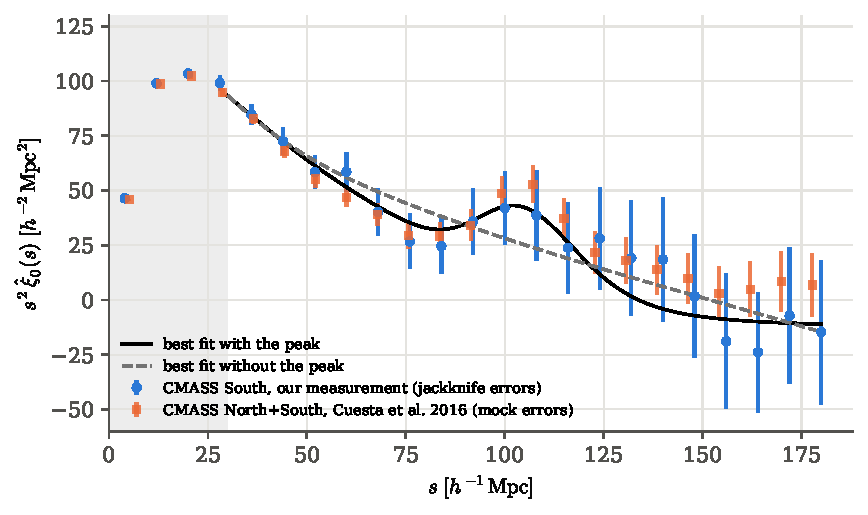
\includegraphics[width=0.95\linewidth]{figures/ch13/cmass_xi_overlay.pdf}
\caption{Our monopole of the southern cap (blue) and the published monopole of the
whole CMASS sample (orange), both times $s^2$. The published separations are rescaled
by $\QpmToOurs$, the ratio of the two fiducial $D_V$, to put them in our coordinates.
Lines: our best fits with and without the acoustic feature. The grey band is outside
the fit range.}
\label{13c:fig:overlay}
\end{figure}

\Cref{13c:fig:overlay} sets the two measurements on one axis. Below $90\,h^{-1}$Mpc
they agree point by point within the error bars.
Both show the bump. Ours is lower between $105$ and $120\,h^{-1}$Mpc, and beyond
$150\,h^{-1}$Mpc our points scatter by more than the published ones, as their error
bars, about twice as large, say they should. The southern cap is part of the whole
sample, so the agreement at small separations is not a test of independent data; it
is a test that our coordinates, weights and estimator reproduce theirs.

\begin{figure}[htbp]
\centering
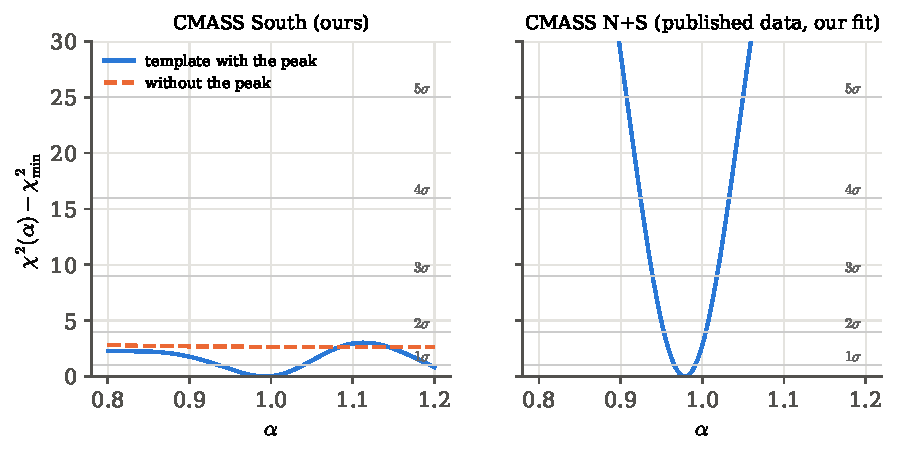
\includegraphics[width=0.95\linewidth]{figures/ch13/cmass_chi2.pdf}
\caption{$\chi^2(\alpha)-\chi^2_{\min}$ for the template with the acoustic feature
(solid) and without it (dashed), for our southern measurement (left) and for the
published monopole of the whole sample refitted with our code (right). Grey lines:
the $\Delta\chi^2=n^2$ levels.}
\label{13c:fig:chi2}
\end{figure}

\paragraph{The published data, refitted.} The right panel of \cref{13c:fig:chi2} is the
textbook case. $\chi^2(\alpha)$ is a deep parabola with its minimum at
$\alpha=\PubAlpha\pm\PubSigAlpha$; the template without a peak is worse by
$\Delta\chi^2=\PubDchi$, a $\PubSignif\sigma$ detection by the rule of
\eqref{11a:eq:dchi2-sigma}. With \eqref{13c:eq:dv-alpha}, our template and their
fiducial distance $D_V^{\rm fid}h=\DvQpm\,h^{-1}$Mpc, this is
$D_V/r_d=\PubDvRd\pm\PubSigDvRd$, against their $13.87\pm\CuestaSigStat$. Our $\alpha$
differs from theirs by almost four per cent while the distances agree to a fraction
of a per cent. Nothing went
wrong: $\alpha$ is not a property of the Universe but of the pair (coordinates,
template), and our template ruler in $h^{-1}$Mpc, $\BaoRdH$ against $147.10\times0.7=102.97$, is
shorter than theirs by the same fraction. Their result is reproduced by an independent code with an independent
template.

\paragraph{Our southern measurement.} The left panel is a different picture. The
curve has a clear minimum at $\alpha=\BaoAlphaBest$, with $\chi^2_{\min}=\BaoChiMin$
for $\CmFitDof$ degrees of freedom, a good fit. But it never rises far: within the
grid it climbs at most $\BaoPlateau$ above its minimum, and the template without a
peak is worse by only $\Delta\chi^2=\BaoDchi$. Anderson et al.\ separated two
questions that a curve like this keeps apart \srcref{Anderson2012}{\S5}.
\begin{itemize}[itemsep=1pt,leftmargin=1.2em]
  \item \emph{Is there a peak?} The gap between the two curves at their minima. Ours is
        $\BaoDchi$, so the acoustic feature is preferred at $\BaoSignif\sigma$. As
        a test (\cref{ch:04}), the null hypothesis is the smooth template, whose
        noise we know: if there were no acoustic feature, would a gain of $\BaoDchi$ or
        more in $\chi^2$ be something to expect? The tail of $\chi^2$ with one degree
        of freedom beyond $2.6$ is $0.11$, one chance in nine, so yes, and the extra
        freedom of $\alpha$ only makes such gains more common. The same tail beyond the
        whole sample's $\PubDchi$ is $10^{-9}$.
  \item \emph{Where is it?} How far the solid curve rises away from its minimum. Near
        the minimum $\Delta\chi^2<1$ for $\BaoLocLo<\alpha<\BaoLocHi$, a local error
        of $\pm\BaoSigLoc$. Farther out the curve flattens into a plateau, because a
        template stretched far from the data's bump puts its own bump where there is
        none, and the smooth terms then fit almost as well as without a bump.
\end{itemize}
The plateau decides the posterior's width. At $\alpha=0.8$ the curve is only
$\BaoEdgeLo$ above its minimum, so $p(\alpha)$ there is still $\BaoEdgeWeight$ of its
peak value, and the standard deviation over the grid, $\sigma_\alpha=\BaoSigAlpha$,
is set as much by the edges of the flat prior as by the data. A wider prior would
give a wider error. This is what a weak detection looks like, and the right summary of
our measurement is two numbers: $\alpha=\BaoAlpha\pm\BaoSigAlpha$ over the prior
$0.8<\alpha<1.2$, or $\pm\BaoSigLoc$ if one accepts that the minimum at
$\BaoAlphaBest$ is the acoustic peak. Through \eqref{13c:eq:dv-alpha},
\begin{equation}
  \frac{D_V(\BaoZeff)}{r_d}=\BaoDvRd\pm\BaoSigDvRd\quad(\text{local: }\pm\BaoSigLocDvRd),
  \qquad\text{Planck: }\BaoPred .
  \label{13c:eq:our-dv}
\end{equation}

\begin{figure}[htbp]
\centering
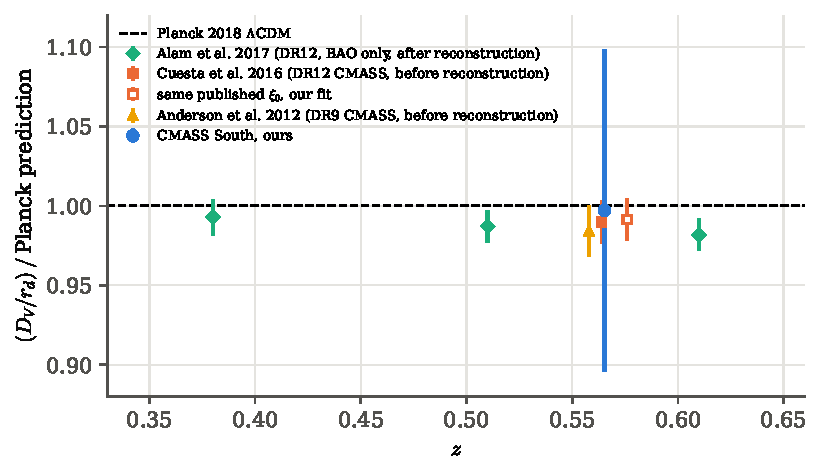
\includegraphics[width=0.92\linewidth]{figures/ch13/cmass_dv.pdf}
\caption{$D_V/r_d$ divided by the Planck 2018 prediction at each redshift. BOSS
results (Anderson et al.\ converted to CAMB's $r_d$; Alam et al.'s $D_M$ and $H$
combined into $D_V$), our refit of the published monopole (open square), and our
southern measurement (blue, with the posterior error over $0.8<\alpha<1.2$). Points at
$z\approx0.57$ are spread slightly in $z$ to be visible.}
\label{13c:fig:dv}
\end{figure}

\Cref{13c:fig:dv,13c:tab:compare} collect the numbers. For Alam et al.'s final
distances we form $D_V/r_d$ from their $D_M\,r_d^{\rm fid}/r_d$ and $H\,r_d/r_d^{\rm
fid}$ with \eqref{11a:eq:dv} and the delta-method error \eqref{11a:eq:dv-error},
using their covariance between the two; they include reconstruction and both
directions, so their errors are smaller, and their bins at $z=0.51$ and $0.61$ bracket
ours.

\begin{table}[htbp]
\centering
\small
\begin{tabular}{@{}llccc@{}}
\toprule
analysis & sample & $z$ & $D_V/r_d$ & Planck\\\midrule
Anderson et al.\ 2012 & DR9 CMASS & $0.57$ & $\AndDvRd\pm\AndSigDvRd$ & $\BaoPredFiftySeven$\\
Cuesta et al.\ 2016 & DR12 CMASS, N+S & $0.57$ & $13.87\pm0.19$ & $\BaoPredFiftySeven$\\
their $\hat\xi_0$, our fit & DR12 CMASS, N+S & $0.57$ & $\PubDvRd\pm\PubSigDvRd$ & $\BaoPredFiftySeven$\\
ours & DR12 CMASS, S & $\BaoZeff$ & $\BaoDvRd\pm\BaoSigDvRd$ & $\BaoPred$\\
Alam et al.\ 2017 & DR12, all & $0.51$ & $\AlamDvB\pm\AlamSdvB$ & $\AlamPredB$\\
Alam et al.\ 2017 & DR12, all & $0.61$ & $\AlamDvC\pm\AlamSdvC$ & $\AlamPredC$\\
\bottomrule
\end{tabular}
\caption{Paper against ours. All values use CAMB's $r_d$ (Anderson et al.'s
$13.44\pm0.22$ converted as in \cref{13c:sec:repro-equation}); the first four are
before reconstruction and from the monopole, Alam et al.'s after reconstruction and
from both directions. The last column is the Planck 2018 prediction at that $z$.}
\label{13c:tab:compare}
\end{table}

\subsection{Why they differ}
\label{13c:sec:repro-why}

Three numbers need explaining: why our error is so much larger than the published one,
why our detection is weaker than expected, and whether our $\alpha$ agrees with
theirs. The distances themselves need little explaining: they agree with each other and
with the Planck prediction to within two standard deviations, the BOSS values sitting
one to two per cent below the prediction.

\paragraph{The area, and the jackknife.} The southern cap is $27\%$ of the area, so by
the mode counting of \cref{13c:sec:jk-check} its errors on $\hat\xi_0$ should be
$\AreaScale$ times the published ones; with the jackknife's slight excess they are
$\ErrRatio$ times. The significance $\sqrt{\Delta\chi^2}$ is the bump's amplitude
divided by its standard error (\cref{11a:eq:dchi2-sigma}), so for a southern cap
with an average bump it would be $\PubSignif/\ErrRatio=\BaoExpSignif\sigma$. We
found $\BaoSignif\sigma$.

\paragraph{A weaker bump than average.} Is $\BaoSignif$ against an expected
$\BaoExpSignif$ a surprise? The estimated amplitude $\hat A$ of the bump scatters from
survey to survey with standard deviation $\sigma_A$, so $\sqrt{\Delta\chi^2}\approx\hat
A/\sigma_A$ scatters by about one unit. Our cap is $\BaoShort$ units below the
expectation; a Gaussian falls that low or lower in about $\BaoShortP\%$ of cases. The
mock surveys of \cref{11a:sec:bao-mocks} showed the same spread from the other side,
where the 2005 detection sat in the upper tail. \Cref{13c:fig:overlay} shows where the
deficit is: our points between $105$ and $120\,h^{-1}$Mpc fall below the published
ones, so the south's bump is narrower and lower than the whole sample's.

\paragraph{Why a weak bump is also badly located.} The width of the $\chi^2$ minimum
is tied to the strength of the detection. Near the best fit, write the model as the
smooth part plus the bump, $B^2\xi_t=B^2(\xi_{\rm nw}+\Delta)$, where $\Delta(s)$ is
the acoustic feature, and suppose the smooth terms absorb the change of $\xi_{\rm nw}$
with $\alpha$, so that only the bump's motion is informative. Then the two curvatures
of $\chi^2$ are
\begin{align}
  \frac{1}{\sigma_\alpha^2}
  &\eqby{1}\Bigl(B^2\,\partial_\alpha\Delta\Bigr)\T\Cmat^{-1}\Bigl(B^2\,\partial_\alpha\Delta\Bigr)
   \eqby{2}B^4\,\bigl(s\Delta'\bigr)\T\Cmat^{-1}\bigl(s\Delta'\bigr),
  \nonumber\\
  \Delta\chi^2
  &\eqby{3}\frac{1}{\sigma_A^2}
   \eqby{4}B^4\,\Delta\T\Cmat^{-1}\Delta ,
  \nonumber\\
  \sigma_\alpha\sqrt{\Delta\chi^2}
  &\eqby{5}\biggl[\frac{\Delta\T\Cmat^{-1}\Delta}{(s\Delta')\T\Cmat^{-1}(s\Delta')}\biggr]^{1/2}.
  \label{13c:eq:sigma-dchi}
\end{align}
\begin{explain}
  \item For a model linear in a parameter near its best fit, $1/\sigma^2$ is the
        derivative vector of the model sandwiched by $\Cmat^{-1}$ (the Fisher matrix
        of a Gaussian mean, \cref{10a:sec:gauss}).
  \item $\partial_\alpha\Delta(\alpha s)=s\,\Delta'(\alpha s)$, evaluated at $\alpha=1$.
  \item \eqref{11a:eq:dchi2-sigma} with the data preferring the full amplitude.
  \item The bump's amplitude $A$ multiplies $B^2\Delta$, so its Fisher information is
        that vector sandwiched by $\Cmat^{-1}$.
  \item Divide the second line by the first, so that $B^4$ cancels, and take the square root.
\end{explain}
The right-hand side depends only on the shape of the bump and of the covariance, not
on how strong the signal is. A bump detected half as strongly is located half as
precisely. The check: $\sigma_\alpha\sqrt{\Delta\chi^2}$ is $\BaoProd$ for our cap
(local width) and $\PubProd$ for the whole sample, equal within the roughness of the
approximation although the covariances come from different methods. So the large
error on our $\alpha$ is not a separate failure; it is the weak detection seen again.
Had our bump been average, the local error would have been about
$\BaoExpSigAlpha$.

\paragraph{Our $\alpha$ against theirs.} Are $\BaoAlphaBest$ (ours, south) and
$\PubAlphaBest$ (the whole sample, same template) consistent? The two are not
independent, since the south is inside the whole sample, so the usual rule of adding
variances does not apply. Treat the whole-sample estimate as the inverse-variance
average of a southern estimate $\alpha_S$ and a northern one $\alpha_N$, independent,
with variances $\sigma_S^2$ and $\sigma_N^2$, and ask for the variance of the
difference $\alpha_S-\alpha_{NS}$.
\begin{align}
  \alpha_{NS}&=\sigma_{NS}^2\Bigl(\frac{\alpha_S}{\sigma_S^2}+\frac{\alpha_N}{\sigma_N^2}\Bigr),
  \qquad \frac{1}{\sigma_{NS}^2}=\frac{1}{\sigma_S^2}+\frac{1}{\sigma_N^2},
  \nonumber\\
  \alpha_S-\alpha_{NS}
  &\eqby{1}\sigma_{NS}^2\Bigl(\frac{1}{\sigma_S^2}+\frac{1}{\sigma_N^2}\Bigr)\alpha_S
   -\sigma_{NS}^2\Bigl(\frac{\alpha_S}{\sigma_S^2}+\frac{\alpha_N}{\sigma_N^2}\Bigr)
   =\frac{\sigma_{NS}^2}{\sigma_N^2}\,(\alpha_S-\alpha_N),
  \nonumber\\
  \Var(\alpha_S-\alpha_{NS})
  &\eqby{2}\frac{\sigma_{NS}^4}{\sigma_N^4}\bigl(\sigma_S^2+\sigma_N^2\bigr)
   \eqby{3}\frac{\sigma_S^4}{\sigma_S^2+\sigma_N^2}
   \eqby{4}\sigma_S^2-\sigma_{NS}^2 .
  \label{13c:eq:subset-diff}
\end{align}
\begin{explain}
  \item Multiply $\alpha_S$ by $1=\sigma_{NS}^2(1/\sigma_S^2+1/\sigma_N^2)$ and
        subtract; the $\alpha_S/\sigma_S^2$ terms cancel.
  \item $\alpha_S$ and $\alpha_N$ are independent, so their variances add.
  \item $\sigma_{NS}^2=\sigma_S^2\sigma_N^2/(\sigma_S^2+\sigma_N^2)$, so
        $\sigma_{NS}^4/\sigma_N^4=\sigma_S^4/(\sigma_S^2+\sigma_N^2)^2$.
  \item $\sigma_S^2-\sigma_{NS}^2=\sigma_S^2\bigl[1-\sigma_N^2/(\sigma_S^2+\sigma_N^2)\bigr]
        =\sigma_S^4/(\sigma_S^2+\sigma_N^2)$.
\end{explain}
A subset's estimate differs from the whole sample's by noise of variance
$\sigma_S^2-\sigma_{NS}^2$, smaller than either naive sum. With the local widths,
$\sqrt{\BaoSigLoc^2-\PubSigLoc^2}=\SigDiffAlpha$, and the difference
$\DiffAlpha$ is a $\DiffPull\sigma$ deviation. The north and south caps really were
analysed separately by BOSS and agreed within $2\sigma$ in DR9 \cite{Ross2012}.

\paragraph{Smaller differences.} Our randoms are $\XiRandRatio$ times the galaxies, not
$50$ (\cref{13c:sec:xi-python}); the shot noise of $RR$ and $DR$ then adds a few per
cent to the variance at the acoustic scale. All analyses in \cref{13c:tab:compare}
except Alam et al.'s are before reconstruction; reconstruction sharpens the bump and
shrinks the error by about a quarter (from $0.19$ to $0.14$ for the whole sample,
\srcref{Cuesta2016}{\S4.4}). The DR9 sample
of Anderson et al.\ is a third of DR12 and partly the same galaxies, so its
agreement with DR12 is again a subset comparison.

\paragraph{Lesson.} Reproducing a BAO distance taught two things that reading the papers
did not. A fitted $\alpha$ is meaningless without its coordinates and its template, and
two analyses that disagree by four per cent in $\alpha$ can agree to a fraction of a
per cent in $D_V/r_d$;
equation \eqref{13c:eq:dv-alpha} is what makes them comparable. And the error on a
peak's position does not follow the area alone. It scales with the inverse of the
detection significance, and that scatters by about one unit from sky to sky. The
southern cap has $27\%$ of the area, which makes the errors on $\xi$ about
$\AreaScale$ times larger, yet its local error on $\alpha$ is $\BaoSigLoc$ against
$\PubSigLoc$ for the whole sample, and its posterior over the prior range is wider
still. A weak detection is also a poor location.
\section{The survey window, and what the full analysis adds}
\label{13c:sec:full}

The galaxy catalogue and the Planck map share one difficulty. Neither covers the whole
sky evenly: the CMB is hidden behind the Galaxy and point sources, and the galaxies
were observed only inside the BOSS footprint, with a density that falls with distance.
For the CMB that difficulty took a whole machinery, the mode-coupling matrix of
\cref{8b:sec:coupling} and its inversion in MASTER (\cref{8b:sec:master},
\cite{Hivon2002}). For the galaxies we never built a coupling matrix, and yet
\cref{13c:fig:overlay} agrees with the published measurement. Where did the window go?

\subsection{The random catalogue is the mask}
\label{13c:sec:window}

\emph{The question.} A survey multiplies the true galaxy density by a window
$W(\bm x)$, the expected number of weighted galaxies per unit volume at $\bm x$ when
there is no clustering. In our analysis $W=\bar n\,w_{\rm FKP}$: zero outside the
footprint and the redshift slice, and shaped inside by $\bar n(z)$ and the FKP weight of
\eqref{13c:eq:final-weights}. What does $W$ do to the expected pair counts?

Count pairs whose separation falls in a thin shell of radius $s$ and width $\delta s$.
Write $\Theta_s(\bm r)$ for the indicator of that shell, $1$ if $s<|\bm r|<s+\delta s$
and $0$ otherwise. The weighted galaxy density has mean $W(\bm x)$ and pair correlation
$\xi$ (\cref{11a:sec:cox-moments}), and the randoms sample $W$ with no correlation.
\begin{align}
  \langle DD(s)\rangle
  &\eqby{1}\int\!\!\int W(\bm x)\,W(\bm y)\,\bigl[1+\xi(|\bm x-\bm y|)\bigr]\,
   \Theta_s(\bm x-\bm y)\,\dd\bm x\,\dd\bm y
  \nonumber\\
  &\eqby{2}\bigl[1+\xi(s)\bigr]\int\!\!\int W(\bm x)\,W(\bm y)\,
   \Theta_s(\bm x-\bm y)\,\dd\bm x\,\dd\bm y ,
  \nonumber\\
  \langle RR(s)\rangle
  &\eqby{3}\int\!\!\int W(\bm x)\,W(\bm y)\,\Theta_s(\bm x-\bm y)\,\dd\bm x\,\dd\bm y,
  \qquad\text{so}\qquad
  \frac{\langle DD(s)\rangle}{\langle RR(s)\rangle}\eqby{4}1+\xi(s).
  \label{13c:eq:window-ratio}
\end{align}
\begin{explain}
  \item The expected number of pairs in two small volumes is the product of the mean
        densities times $1+\xi$ (\cref{11a:eq:pair-count}), summed over all pairs of
        volumes whose separation is in the shell.
  \item Inside a thin shell $|\bm x-\bm y|\approx s$, so $\xi$ is the same for every
        pair and comes out of the integral.
  \item The randoms have the same mean density shape $W$ and no clustering.
  \item The double integral is the same in both; it cancels. (The normalisations of
        \eqref{13c:eq:weighted-counts} make the total pair numbers agree.)
\end{explain}
The double integral is the window's own pair count: how many pairs at separation $s$
the footprint can hold at all. It is the configuration-space twin of the mask's power
spectrum $\mathcal W_\ell$ that builds the coupling matrix in
\srcref{Hivon}{(14), (A31)}. Because the correlation function depends only on the separation,
and a thin shell fixes the separation, the window multiplies each bin by its own
number and mixes nothing: dividing by $RR$ undoes it bin by bin. The randoms are the
mask, and $RR$ is its coupling ``matrix'', which here is diagonal. The Landy--Szalay
combination \eqref{13c:eq:ls} keeps this property and also cancels the leading edge
terms in the variance (\cref{11a:sec:xi-expansion}).

\emph{Why the power spectrum is different.} The FKP estimator of \cref{11a:sec:fkp}
Fourier transforms the weighted density on a grid. Multiplication by $W$ in
configuration space is a convolution in Fourier space, so the measured power at $\bm k$
is the true power averaged over neighbouring wavevectors with weight $|\tilde
W(\bm k-\bm k')|^2$. Every $k$-bin mixes with its neighbours, exactly as the mask mixes
multipoles on the sphere, and a sharp feature such as the acoustic wiggles is
smoothed (\cref{13c:fig:window}). A $P(k)$ analysis must therefore convolve the model
with the window, the analogue of the forward-modelling route of MASTER, before
comparing it with data.

\paragraph{Example: how much a window smooths a wiggle.}
Take a wiggle $1+A\sin(kr_d)$ and a window whose $|\tilde W|^2$, normalised to unit
integral, is a Gaussian of width $\sigma_k$ in $k$. The convolved
wiggle is the average of $\sin\bigl((k-q)r_d\bigr)$ over $q\sim\Normal(0,\sigma_k^2)$.
Write the sine as the imaginary part of $e^{i(k-q)r_d}$; the average of $e^{-iqr_d}$
over a Gaussian is $e^{-\sigma_k^2r_d^2/2}$ (complete the square in the exponent), a
real number, so the average is $\sin(kr_d)\,e^{-\sigma_k^2r_d^2/2}$ and the wiggle
survives with amplitude $A\,e^{-\sigma_k^2r_d^2/2}$. A survey $L\approx1\,h^{-1}$Gpc deep has
$\sigma_k\sim1/L$, and with $r_d\approx100\,h^{-1}$Mpc the factor is
$e^{-0.005}$: a large survey barely blurs the BAO. A thin slice $100\,h^{-1}$Mpc deep
in one direction has $\sigma_kr_d\sim1$ along it and keeps only $e^{-1/2}\approx60\%$
of the wiggle in that direction. Pair counts would see the same peak at full height.

\paragraph{Where the cancellation fails.} Equation \eqref{13c:eq:window-ratio} assumed that
the randoms trace the true window. They do not if the mean density is itself estimated
from the same galaxies: the randoms' redshifts are drawn from the galaxies
(\cref{13c:sec:files}), and the total number is normalised to the observed number.
Both remove the large-scale fluctuations that the survey's own volume contains, the
integral constraint of \cref{11a:sec:integral-constraint}, which pulls $\hat\xi$ down
by a nearly constant amount; the term $a_0$ in the fit \eqref{11a:eq:xi-fit} absorbs
it. Ross et al.\ compared ways of giving the randoms their redshifts on mock catalogues
and found that drawing them from the galaxies (``shuffling'') biased the clustering
least \srcref{Ross2012}{\S6.1}.

\begin{figure}[htbp]
\centering
\begin{tikzpicture}[scale=0.92]
  \begin{scope}
    \draw[formblue,thick,fill=formblue!8]
      (0,0) -- (3.4,0.2) -- (3.8,1.6) -- (3.0,2.9) -- (1.2,3.1) -- (-0.2,2.2) -- cycle;
    \fill[white,draw=formblue,thick] (2.6,0.55) circle (0.28);   %
    \fill[fibreorange] (2.6,1.9) circle (1.8pt);
    \draw[bdryred,thick] (2.6,1.9) circle (1.25);
    \draw[bdryred,thick] (2.6,1.9) circle (1.45);
    \node[lbl,anchor=north] at (1.8,-0.55) {shell of radius $s$ in the footprint};
    \node[lbl] at (0.7,2.2) {$W\neq0$};
  \end{scope}
  \begin{scope}[xshift=5.6cm]
    \draw[->,black!60] (0,0) -- (5.2,0) node[lbl,anchor=north east] at (5.2,-0.05) {$k$};
    \draw[->,black!60] (0,0) -- (0,3.0) node[lbl,anchor=east] at (0,2.8) {$P(k)$};
    \draw[form,thick,domain=0.2:5,samples=200]
      plot (\x,{1.5+0.7*sin(deg(4*\x))});
    \draw[bdryred,thick,dashed,domain=0.2:5,samples=200]
      plot (\x,{1.5+0.7*exp(-0.5)*sin(deg(4*\x))});
    \node[lbl,anchor=north] at (2.6,-0.55) {true (blue), window-convolved (red)};
  \end{scope}
\end{tikzpicture}
\caption{The window in two spaces. Left: in configuration space, pairs at one
separation are counted in a shell; the footprint (blue, with a masked hole) cuts the
shell, but it cuts the galaxy pairs and the random pairs alike, so their ratio is
untouched. Right: in Fourier space the window convolves the spectrum; for a Gaussian
window of width $\sigma_k$ a wiggle of period $2\pi/r_d$ keeps the fraction
$e^{-\sigma_k^2r_d^2/2}$ of its amplitude (drawn for $\sigma_kr_d=1$).}
\label{13c:fig:window}
\end{figure}

\subsection{The full analysis, and what our shortcuts cost}
\label{13c:sec:nerfs}

Each step of our pipeline has a research-grade version. \Cref{13c:tab:nerfs} lists
them with the price of the shortcut; the largest prices are the area, which costs a
factor of about two in every error, and the absence of mocks, which makes the error
bars themselves uncertain by some tens of per cent.

\begin{table}[htbp]
\centering
\small
\begin{tabular}{@{}>{\raggedright\arraybackslash}p{0.16\linewidth}>{\raggedright\arraybackslash}p{0.3\linewidth}>{\raggedright\arraybackslash}p{0.46\linewidth}@{}}
\toprule
step & ours & BOSS DR12, and the cost of our choice\\\midrule
sky & southern cap, $27\%$ of the area & both caps \cite{Cuesta2016}; errors $\AreaScale$ times larger, detection $\BaoSignif\sigma$ instead of $\PubSignif\sigma$\\
randoms & $\XiRandRatio$ per galaxy in the counts & $50$ per galaxy \cite{Reid2016}; a few per cent more variance\\
covariance & $\CmNjk$ jackknife regions & about a thousand quick-particle-mesh (QPM) mocks ($956$ for CMASS) and a second set as a check; our errors uncertain by tens of per cent, Hartlap factor only a guide\\
statistic & monopole only & monopole and quadrupole; we measure $D_V$ only, not $D_M$ and $H$ separately\\
reconstruction & none & displacements estimated from the density field and undone; our errors about $25\%$ larger\\
template & fixed $\Sigma_{\rm nl}=8\,h^{-1}$Mpc & damping calibrated on mocks, systematic error budget for template and fiducial cosmology\\
blinding & none & catalogue-level blinding, now standard \srcref{DESI2024VI}{\S2.3.1}\\
\bottomrule
\end{tabular}
\caption{Our analysis of CMASS South against the published BOSS analysis.}
\label{13c:tab:nerfs}
\end{table}

All of it ran at laptop scale: the fully weighted pair counts took $\XiTime$\,s on
$\XiNproc$ cores, and the fits a few seconds. The full DR12 random catalogues of both
caps, at $50$ times the galaxies, would need more than $4\,$GB of downloads and several
hundred times our pair-counting time, because the number of random pairs within
$184\,h^{-1}$Mpc grows as the number of randoms times their density.

Two further summaries of the same catalogue follow from earlier chapters, and our
analysis did not compute them. The power-spectrum monopole with FKP weights (\cref{11a:sec:fkp})
measures the same wiggles in Fourier space, and \cref{13c:sec:window} says what it
needs: the model convolved with the window of our footprint. The Betti curves of the
smoothed galaxy density (\cref{12b:sec:grf3d}) would test the morphology of the
cosmic web, but their null distribution, like that of the CMB sky in
\cref{13b:sec:question}, must come from mocks that pass through the same window: a
mask changes the topology of every excursion set it cuts.

\begin{inpractice}[verification and research in a BAO analysis]
Two of our checks were verifications: refitting the published monopole
(\cref{13c:sec:repro-side}) tested our fitting code against a known answer, and
comparing jackknife errors with mock errors (\cref{13c:sec:jk-check}) tested an error
method against a better one. In the research analysis the same Monte Carlo machinery is
the instrument. Thousands of mock surveys, each with the real footprint, density and
fibre collisions, give the covariance; the same mocks measure whether reconstruction
or the template shifts $\alpha$, which sets the systematic error; and the fitted
$\alpha$ of each mock gives the sampling distribution of $\hat\alpha$, against which
non-Gaussian error behaviour like that of our \cref{13c:fig:chi2} is calibrated
\cite{Cuesta2016,Alam2017}. DESI adds blinding: the catalogue is shifted in a hidden way
until the analysis choices are frozen, so that agreement with a favoured model cannot
steer them \srcref{DESI2024VI}{\S2.3.1}.
\end{inpractice}

\begin{recap}
\begin{itemize}[itemsep=1pt,leftmargin=1.2em]
  \item A galaxy catalogue becomes a set of positions through a fiducial
        distance--redshift relation; the error made by choosing the wrong one is
        exactly what the dilation $\alpha$ measures.
  \item Weights restore the galaxies the survey could not observe properly (close
        pairs, redshift failures, stars and seeing) and the FKP weight balances
        signal and shot noise; the randoms carry only the FKP weight because they
        already trace the survey's completeness.
  \item The Landy--Szalay estimator with weighted counts divides out the survey window
        bin by bin, because in a thin shell the correlation function is constant; in
        Fourier space the same window convolves the spectrum and must be modelled.
  \item Counting pairs region by region gives every leave-one-region-out count by
        inclusion--exclusion, and with them the jackknife covariance
        $\frac{N-1}{N}\sum_k(\hat{\bm\xi}_{-k}-\bar{\bm\xi})(\hat{\bm\xi}_{-k}-\bar{\bm\xi})\T$,
        exact for a mean and biased upward otherwise; on CMASS South it agrees with
        scaled mock errors to $\ErrRatioOverArea$.
  \item A fitted $\alpha$ becomes a distance through
        $D_V/r_d=\alpha\,D_V^{\rm fid}/r_d^{\rm tmpl}$; the ruler's name and the
        coordinates must be identified before numbers are compared.
  \item CMASS South shows the acoustic peak at $\BaoSignif\sigma$ and gives
        $D_V/r_d=\BaoDvRd\pm\BaoSigDvRd$, consistent with BOSS and Planck; the whole
        sample, refitted with our code, gives $\PubDvRd\pm\PubSigDvRd$ at
        $\PubSignif\sigma$, as published.
  \item A weak detection is also a poor location, $\sigma_\alpha\sqrt{\Delta\chi^2}$
        being fixed by the shape of the bump; and a subset differs from its parent
        sample by noise of variance $\sigma_S^2-\sigma_{NS}^2$.
\end{itemize}
\end{recap}
\providecommand{\FourBScPgvFive}{}\renewcommand{\FourBScPgvFive}{1.36\times10^{-5}}
\providecommand{\FourBScZgvFive}{}\renewcommand{\FourBScZgvFive}{4.20}
\providecommand{\FourBScPlocFive}{}\renewcommand{\FourBScPlocFive}{2.87\times10^{-7}}
\providecommand{\FourBScBtot}{}\renewcommand{\FourBScBtot}{3000}
\providecommand{\FourBScSlope}{}\renewcommand{\FourBScSlope}{30}
\providecommand{\FourBScSigM}{}\renewcommand{\FourBScSigM}{1.5}
\providecommand{\FourBScNmass}{}\renewcommand{\FourBScNmass}{201}
\providecommand{\FourBScToys}{}\renewcommand{\FourBScToys}{20000}
\providecommand{\FourBScMobs}{}\renewcommand{\FourBScMobs}{142.50}
\providecommand{\FourBScMuObs}{}\renewcommand{\FourBScMuObs}{42}
\providecommand{\FourBScQobs}{}\renewcommand{\FourBScQobs}{10.79}
\providecommand{\FourBScZloc}{}\renewcommand{\FourBScZloc}{3.28}
\providecommand{\FourBScPloc}{}\renewcommand{\FourBScPloc}{5.10\times10^{-4}}
\providecommand{\FourBScPglob}{}\renewcommand{\FourBScPglob}{0.0159}
\providecommand{\FourBScPglobErr}{}\renewcommand{\FourBScPglobErr}{0.0009}
\providecommand{\FourBScZglob}{}\renewcommand{\FourBScZglob}{2.15}
\providecommand{\FourBScTrials}{}\renewcommand{\FourBScTrials}{31.3}
\providecommand{\FourBScNzeroHundred}{}\renewcommand{\FourBScNzeroHundred}{2.78}
\providecommand{\FourBScNzeroAll}{}\renewcommand{\FourBScNzeroAll}{2.804}
\providecommand{\FourBScNone}{}\renewcommand{\FourBScNone}{3.60}
\providecommand{\FourBScPgv}{}\renewcommand{\FourBScPgv}{0.0167}
\providecommand{\FourBScFracZero}{}\renewcommand{\FourBScFracZero}{0.508}
\providecommand{\FourBScPfourMC}{}\renewcommand{\FourBScPfourMC}{0.0234}
\providecommand{\FourBScPfourTh}{}\renewcommand{\FourBScPfourTh}{0.0228}
\providecommand{\FourBScPthreeGlob}{}\renewcommand{\FourBScPthreeGlob}{0.040}
\providecommand{\FourBScTrialsThreeAsym}{}\renewcommand{\FourBScTrialsThreeAsym}{28}
\providecommand{\HyyNData}{}\renewcommand{\HyyNData}{76394}
\providecommand{\HyyNCat}{}\renewcommand{\HyyNCat}{8582}
\providecommand{\HyyNTrig}{}\renewcommand{\HyyNTrig}{7798424}
\providecommand{\HyyNTwo}{}\renewcommand{\HyyNTwo}{979404}
\providecommand{\HyyNIso}{}\renewcommand{\HyyNIso}{362972}
\providecommand{\HyyNKin}{}\renewcommand{\HyyNKin}{322243}
\providecommand{\HyyNAll}{}\renewcommand{\HyyNAll}{7798424}
\providecommand{\HyySigExp}{}\renewcommand{\HyySigExp}{397.9}
\providecommand{\HyySigCat}{}\renewcommand{\HyySigCat}{58.8}
\providecommand{\HyySigTrig}{}\renewcommand{\HyySigTrig}{610.9}
\providecommand{\HyySigTwo}{}\renewcommand{\HyySigTwo}{485.2}
\providecommand{\HyySigIso}{}\renewcommand{\HyySigIso}{430}
\providecommand{\HyySigKin}{}\renewcommand{\HyySigKin}{398.1}
\providecommand{\HyySigAll}{}\renewcommand{\HyySigAll}{610.9}
\providecommand{\HyyEffSig}{}\renewcommand{\HyyEffSig}{0.651}
\providecommand{\HyyRelSyst}{}\renewcommand{\HyyRelSyst}{0.0086}
\providecommand{\HyyNA}{}\renewcommand{\HyyNA}{4227}
\providecommand{\HyyNB}{}\renewcommand{\HyyNB}{14804}
\providecommand{\HyyNC}{}\renewcommand{\HyyNC}{21876}
\providecommand{\HyyND}{}\renewcommand{\HyyND}{35487}
\providecommand{\HyySigggH}{}\renewcommand{\HyySigggH}{357.2}
\providecommand{\HyySigVBF}{}\renewcommand{\HyySigVBF}{29.9}
\providecommand{\HyySigWH}{}\renewcommand{\HyySigWH}{5.6}
\providecommand{\HyySigZH}{}\renewcommand{\HyySigZH}{5.3}
\providecommand{\HyyCBmean}{}\renewcommand{\HyyCBmean}{125}
\providecommand{\HyyCBsig}{}\renewcommand{\HyyCBsig}{2.467}
\providecommand{\HyyCBalpha}{}\renewcommand{\HyyCBalpha}{1.88}
\providecommand{\HyyCBn}{}\renewcommand{\HyyCBn}{10.3}
\providecommand{\HyyGmean}{}\renewcommand{\HyyGmean}{124.9}
\providecommand{\HyyGsig}{}\renewcommand{\HyyGsig}{2.6}
\providecommand{\HyyFWHM}{}\renewcommand{\HyyFWHM}{5.81}
\providecommand{\HyyFWHMratio}{}\renewcommand{\HyyFWHMratio}{2.35}
\providecommand{\HyyStot}{}\renewcommand{\HyyStot}{397.9}
\providecommand{\HyyTailFrac}{}\renewcommand{\HyyTailFrac}{3.3}
\providecommand{\HyyGaussTail}{}\renewcommand{\HyyGaussTail}{2.3}
\providecommand{\HyyCBsigCat}{}\renewcommand{\HyyCBsigCat}{1.825}
\providecommand{\HyyCBsigRest}{}\renewcommand{\HyyCBsigRest}{2.58}
\providecommand{\HyyDevExpOne}{}\renewcommand{\HyyDevExpOne}{78.3}
\providecommand{\HyyNdfExpOne}{}\renewcommand{\HyyNdfExpOne}{53}
\providecommand{\HyyPfitExpOne}{}\renewcommand{\HyyPfitExpOne}{0.013}
\providecommand{\HyyDevPow}{}\renewcommand{\HyyDevPow}{63.2}
\providecommand{\HyyNdfPow}{}\renewcommand{\HyyNdfPow}{53}
\providecommand{\HyyPfitPow}{}\renewcommand{\HyyPfitPow}{0.16}
\providecommand{\HyyDevExpTwo}{}\renewcommand{\HyyDevExpTwo}{58.4}
\providecommand{\HyyNdfExpTwo}{}\renewcommand{\HyyNdfExpTwo}{52}
\providecommand{\HyyPfitExpTwo}{}\renewcommand{\HyyPfitExpTwo}{0.252}
\providecommand{\HyyDevBernThree}{}\renewcommand{\HyyDevBernThree}{54.7}
\providecommand{\HyyNdfBernThree}{}\renewcommand{\HyyNdfBernThree}{51}
\providecommand{\HyyPfitBernThree}{}\renewcommand{\HyyPfitBernThree}{0.337}
\providecommand{\HyyDevExpThree}{}\renewcommand{\HyyDevExpThree}{54.5}
\providecommand{\HyyNdfExpThree}{}\renewcommand{\HyyNdfExpThree}{51}
\providecommand{\HyyPfitExpThree}{}\renewcommand{\HyyPfitExpThree}{0.342}
\providecommand{\HyyDevBernFour}{}\renewcommand{\HyyDevBernFour}{54.2}
\providecommand{\HyyNdfBernFour}{}\renewcommand{\HyyNdfBernFour}{50}
\providecommand{\HyyPfitBernFour}{}\renewcommand{\HyyPfitBernFour}{0.318}
\providecommand{\HyyDevExpFour}{}\renewcommand{\HyyDevExpFour}{54.3}
\providecommand{\HyyNdfExpFour}{}\renewcommand{\HyyNdfExpFour}{50}
\providecommand{\HyyPfitExpFour}{}\renewcommand{\HyyPfitExpFour}{0.315}
\providecommand{\HyyDevBernFive}{}\renewcommand{\HyyDevBernFive}{53.4}
\providecommand{\HyyNdfBernFive}{}\renewcommand{\HyyNdfBernFive}{49}
\providecommand{\HyyPfitBernFive}{}\renewcommand{\HyyPfitBernFive}{0.308}
\providecommand{\HyyTruthSBernFive}{}\renewcommand{\HyyTruthSBernFive}{496}
\providecommand{\HyyTruthSExpFour}{}\renewcommand{\HyyTruthSExpFour}{462}
\providecommand{\HyySpurExpOne}{}\renewcommand{\HyySpurExpOne}{707.9}
\providecommand{\HyySpurRelExpOne}{}\renewcommand{\HyySpurRelExpOne}{4.43}
\providecommand{\HyySpurPow}{}\renewcommand{\HyySpurPow}{245.8}
\providecommand{\HyySpurRelPow}{}\renewcommand{\HyySpurRelPow}{2.17}
\providecommand{\HyySpurExpTwo}{}\renewcommand{\HyySpurExpTwo}{273.8}
\providecommand{\HyySpurRelExpTwo}{}\renewcommand{\HyySpurRelExpTwo}{2.42}
\providecommand{\HyySpurBernThree}{}\renewcommand{\HyySpurBernThree}{98.1}
\providecommand{\HyySpurRelBernThree}{}\renewcommand{\HyySpurRelBernThree}{0.71}
\providecommand{\HyySpurExpThree}{}\renewcommand{\HyySpurExpThree}{218.6}
\providecommand{\HyySpurRelExpThree}{}\renewcommand{\HyySpurRelExpThree}{1.19}
\providecommand{\HyySpurBernFour}{}\renewcommand{\HyySpurBernFour}{79.3}
\providecommand{\HyySpurRelBernFour}{}\renewcommand{\HyySpurRelBernFour}{0.41}
\providecommand{\HyySpurExpFour}{}\renewcommand{\HyySpurExpFour}{40.8}
\providecommand{\HyySpurRelExpFour}{}\renewcommand{\HyySpurRelExpFour}{0.29}
\providecommand{\HyySpurBernFive}{}\renewcommand{\HyySpurBernFive}{15.6}
\providecommand{\HyySpurRelBernFive}{}\renewcommand{\HyySpurRelBernFive}{0.06}
\providecommand{\HyySigmaS}{}\renewcommand{\HyySigmaS}{150}
\providecommand{\HyyChosen}{}\renewcommand{\HyyChosen}{BernFive}
\providecommand{\HyySspurChosen}{}\renewcommand{\HyySspurChosen}{15.6}
\providecommand{\HyyMmax}{}\renewcommand{\HyyMmax}{124.5}
\providecommand{\HyyZloc}{}\renewcommand{\HyyZloc}{2.77}
\providecommand{\HyyPloc}{}\renewcommand{\HyyPloc}{0.002846}
\providecommand{\HyyZlocStat}{}\renewcommand{\HyyZlocStat}{2.77}
\providecommand{\HyyMmaxStat}{}\renewcommand{\HyyMmaxStat}{124.5}
\providecommand{\HyyZoneTwoFive}{}\renewcommand{\HyyZoneTwoFive}{2.74}
\providecommand{\HyyZexpOneTwoFive}{}\renewcommand{\HyyZexpOneTwoFive}{2.15}
\providecommand{\HyyMuMax}{}\renewcommand{\HyyMuMax}{1.28}
\providecommand{\HyyQmax}{}\renewcommand{\HyyQmax}{7.6}
\providecommand{\HyyBhatTot}{}\renewcommand{\HyyBhatTot}{76390}
\providecommand{\HyyMsecond}{}\renewcommand{\HyyMsecond}{143}
\providecommand{\HyyZsecond}{}\renewcommand{\HyyZsecond}{2.71}
\providecommand{\HyyMuSecond}{}\renewcommand{\HyyMuSecond}{1.17}
\providecommand{\HyyZsumsb}{}\renewcommand{\HyyZsumsb}{3.41}
\providecommand{\HyyBeta}{}\renewcommand{\HyyBeta}{1527}
\providecommand{\HyyZgaussForm}{}\renewcommand{\HyyZgaussForm}{3.44}
\providecommand{\HyySwin}{}\renewcommand{\HyySwin}{397.9}
\providecommand{\HyyZAdegOne}{}\renewcommand{\HyyZAdegOne}{2.88}
\providecommand{\HyyKeepDegOne}{}\renewcommand{\HyyKeepDegOne}{0.79}
\providecommand{\HyyZAdegTwo}{}\renewcommand{\HyyZAdegTwo}{2.87}
\providecommand{\HyyKeepDegTwo}{}\renewcommand{\HyyKeepDegTwo}{0.74}
\providecommand{\HyyZAdegThree}{}\renewcommand{\HyyZAdegThree}{2.51}
\providecommand{\HyyKeepDegThree}{}\renewcommand{\HyyKeepDegThree}{0.55}
\providecommand{\HyyZAdegFour}{}\renewcommand{\HyyZAdegFour}{2.5}
\providecommand{\HyyKeepDegFour}{}\renewcommand{\HyyKeepDegFour}{0.55}
\providecommand{\HyyZAdegFive}{}\renewcommand{\HyyZAdegFive}{2.16}
\providecommand{\HyyKeepDegFive}{}\renewcommand{\HyyKeepDegFive}{0.41}
\providecommand{\HyyZAdegSix}{}\renewcommand{\HyyZAdegSix}{2.01}
\providecommand{\HyyKeepDegSix}{}\renewcommand{\HyyKeepDegSix}{0.35}
\providecommand{\HyyZAknown}{}\renewcommand{\HyyZAknown}{3.39}
\providecommand{\HyyMuHat}{}\renewcommand{\HyyMuHat}{1.28}
\providecommand{\HyyMuLo}{}\renewcommand{\HyyMuLo}{0.49}
\providecommand{\HyyMuHi}{}\renewcommand{\HyyMuHi}{0.55}
\providecommand{\HyyMuStatLo}{}\renewcommand{\HyyMuStatLo}{0.46}
\providecommand{\HyyMuStatHi}{}\renewcommand{\HyyMuStatHi}{0.46}
\providecommand{\HyySigTot}{}\renewcommand{\HyySigTot}{0.52}
\providecommand{\HyySigStat}{}\renewcommand{\HyySigStat}{0.46}
\providecommand{\HyySigSyst}{}\renewcommand{\HyySigSyst}{0.24}
\providecommand{\HyyThY}{}\renewcommand{\HyyThY}{-0}
\providecommand{\HyyThSig}{}\renewcommand{\HyyThSig}{0.03}
\providecommand{\HyyThM}{}\renewcommand{\HyyThM}{-0.3}
\providecommand{\HyyThSS}{}\renewcommand{\HyyThSS}{-0}
\providecommand{\HyyMhat}{}\renewcommand{\HyyMhat}{124.5}
\providecommand{\HyyMhatLo}{}\renewcommand{\HyyMhatLo}{1.4}
\providecommand{\HyyMhatHi}{}\renewcommand{\HyyMhatHi}{1.4}
\providecommand{\HyyMhatStat}{}\renewcommand{\HyyMhatStat}{124.5}
\providecommand{\HyyMhatStatLo}{}\renewcommand{\HyyMhatStatLo}{0.9}
\providecommand{\HyyMhatStatHi}{}\renewcommand{\HyyMhatStatHi}{0.8}
\providecommand{\HyyLimObsOneTwoFive}{}\renewcommand{\HyyLimObsOneTwoFive}{2.24}
\providecommand{\HyyLimExpOneTwoFive}{}\renewcommand{\HyyLimExpOneTwoFive}{0.96}
\providecommand{\HyyLimExpMin}{}\renewcommand{\HyyLimExpMin}{0.83}
\providecommand{\HyyLimExpMax}{}\renewcommand{\HyyLimExpMax}{1.33}
\providecommand{\HyyNexcl}{}\renewcommand{\HyyNexcl}{19}
\providecommand{\HyyNmlim}{}\renewcommand{\HyyNmlim}{41}
\providecommand{\HyyExclRanges}{}\renewcommand{\HyyExclRanges}{112--119, 130--138, 149--150}
\providecommand{\HyyLimObsOneFourty}{}\renewcommand{\HyyLimObsOneFourty}{1.96}
\providecommand{\HyyLimExpOneFourty}{}\renewcommand{\HyyLimExpOneFourty}{0.93}
\providecommand{\HyySigmaAOneFourty}{}\renewcommand{\HyySigmaAOneFourty}{0.477}
\providecommand{\HyySigmaAOneTwoFive}{}\renewcommand{\HyySigmaAOneTwoFive}{0.491}
\providecommand{\HyyBandCoefMed}{}\renewcommand{\HyyBandCoefMed}{1.94}
\providecommand{\HyyZAincl}{}\renewcommand{\HyyZAincl}{2.16}
\providecommand{\HyyZAcat}{}\renewcommand{\HyyZAcat}{2.26}
\providecommand{\HyyZOincl}{}\renewcommand{\HyyZOincl}{2.71}
\providecommand{\HyyZOcat}{}\renewcommand{\HyyZOcat}{2.99}
\providecommand{\HyyMuOincl}{}\renewcommand{\HyyMuOincl}{1.25}
\providecommand{\HyyMuOcat}{}\renewcommand{\HyyMuOcat}{1.31}
\providecommand{\HyySbCat}{}\renewcommand{\HyySbCat}{0.344}
\providecommand{\HyySbRest}{}\renewcommand{\HyySbRest}{0.25}
\providecommand{\HyyNcat}{}\renewcommand{\HyyNcat}{8582}
\providecommand{\HyyNrest}{}\renewcommand{\HyyNrest}{67812}
\providecommand{\HyyScat}{}\renewcommand{\HyyScat}{58.8}
\providecommand{\HyySrest}{}\renewcommand{\HyySrest}{339.1}
\providecommand{\HyyToyQobs}{}\renewcommand{\HyyToyQobs}{7.7}
\providecommand{\HyyToyZobs}{}\renewcommand{\HyyToyZobs}{2.77}
\providecommand{\HyyToyMobs}{}\renewcommand{\HyyToyMobs}{124.5}
\providecommand{\HyyToyNbkg}{}\renewcommand{\HyyToyNbkg}{4000}
\providecommand{\HyyToyFracZero}{}\renewcommand{\HyyToyFracZero}{0.508}
\providecommand{\HyyToyPfour}{}\renewcommand{\HyyToyPfour}{0.0228}
\providecommand{\HyyToyPfourTh}{}\renewcommand{\HyyToyPfourTh}{0.0228}
\providecommand{\HyyToyPnine}{}\renewcommand{\HyyToyPnine}{0.0012}
\providecommand{\HyyToyPnineTh}{}\renewcommand{\HyyToyPnineTh}{0.0013}
\providecommand{\HyyToyNexceed}{}\renewcommand{\HyyToyNexceed}{229}
\providecommand{\HyyToyPglob}{}\renewcommand{\HyyToyPglob}{0.0572}
\providecommand{\HyyToyPglobErr}{}\renewcommand{\HyyToyPglobErr}{0.0037}
\providecommand{\HyyENhundred}{}\renewcommand{\HyyENhundred}{2.14}
\providecommand{\HyyENall}{}\renewcommand{\HyyENall}{2.06}
\providecommand{\HyyENoneAll}{}\renewcommand{\HyyENoneAll}{1.62}
\providecommand{\HyyNone}{}\renewcommand{\HyyNone}{2.75}
\providecommand{\HyyPlocObs}{}\renewcommand{\HyyPlocObs}{0.002764}
\providecommand{\HyyPgvObs}{}\renewcommand{\HyyPgvObs}{0.0613}
\providecommand{\HyyZgvObs}{}\renewcommand{\HyyZgvObs}{1.54}
\providecommand{\HyyTrialsObs}{}\renewcommand{\HyyTrialsObs}{22.2}
\providecommand{\HyyTrialsAsym}{}\renewcommand{\HyyTrialsAsym}{20.1}
\providecommand{\HyyPgvFull}{}\renewcommand{\HyyPgvFull}{0.06293}
\providecommand{\HyyZgvFull}{}\renewcommand{\HyyZgvFull}{1.53}
\providecommand{\HyyZlocFull}{}\renewcommand{\HyyZlocFull}{2.77}
\providecommand{\HyyPthreeGlobToy}{}\renewcommand{\HyyPthreeGlobToy}{0.032}
\providecommand{\HyyPthreeGlobGV}{}\renewcommand{\HyyPthreeGlobGV}{0.032}
\providecommand{\HyyToyZAsb}{}\renewcommand{\HyyToyZAsb}{2.16}
\providecommand{\HyyToyZmedSb}{}\renewcommand{\HyyToyZmedSb}{2.15}
\providecommand{\HyyToyZsbLo}{}\renewcommand{\HyyToyZsbLo}{1.14}
\providecommand{\HyyToyZsbHi}{}\renewcommand{\HyyToyZsbHi}{3.13}
\providecommand{\HyyToyPsbFive}{}\renewcommand{\HyyToyPsbFive}{0.002}
\providecommand{\HyyLimToyOneFourty}{}\renewcommand{\HyyLimToyOneFourty}{1.05}
\providecommand{\HyyLimAsymOneFourty}{}\renewcommand{\HyyLimAsymOneFourty}{1.07}
\providecommand{\HyyNlimToys}{}\renewcommand{\HyyNlimToys}{1000}
\providecommand{\HyySigAstatOneFourty}{}\renewcommand{\HyySigAstatOneFourty}{0.438}
\providecommand{\HyyQtMuTest}{}\renewcommand{\HyyQtMuTest}{0.5}
\providecommand{\HyyAtlasZcat}{}\renewcommand{\HyyAtlasZcat}{2.93}
\providecommand{\HyyAtlasZincl}{}\renewcommand{\HyyAtlasZincl}{2.5}
\providecommand{\HyyAtlasS}{}\renewcommand{\HyyAtlasS}{190.1}
\providecommand{\HyyAtlasND}{}\renewcommand{\HyyAtlasND}{59039}
\providecommand{\HyyAtlasSperL}{}\renewcommand{\HyyAtlasSperL}{17.8}
\providecommand{\HyyAtlasBetaPerL}{}\renewcommand{\HyyAtlasBetaPerL}{92}
\providecommand{\HyyAtlasSigma}{}\renewcommand{\HyyAtlasSigma}{1.66}
\providecommand{\HyyAtlasProduced}{}\renewcommand{\HyyAtlasProduced}{482}
\providecommand{\HyyAtlasEff}{}\renewcommand{\HyyAtlasEff}{0.39}
\providecommand{\HyyAtlasZperL}{}\renewcommand{\HyyAtlasZperL}{0.76}
\providecommand{\HyyAtlasMuPull}{}\renewcommand{\HyyAtlasMuPull}{1.6}
\providecommand{\HyyOurZformula}{}\renewcommand{\HyyOurZformula}{3.44}
\providecommand{\HyyOurXS}{}\renewcommand{\HyyOurXS}{114}
\providecommand{\HyyOurProduced}{}\renewcommand{\HyyOurProduced}{1149}
\providecommand{\HyyOurEff}{}\renewcommand{\HyyOurEff}{0.35}
\providecommand{\HyyOurSperL}{}\renewcommand{\HyyOurSperL}{39.5}
\providecommand{\HyyOurBetaPerL}{}\renewcommand{\HyyOurBetaPerL}{152}
\providecommand{\HyyOurFWHM}{}\renewcommand{\HyyOurFWHM}{5.81}
\providecommand{\HyyOurZperL}{}\renewcommand{\HyyOurZperL}{0.68}
\providecommand{\HyyXSratio}{}\renewcommand{\HyyXSratio}{2.5}
\providecommand{\HyyLumiForFive}{}\renewcommand{\HyyLumiForFive}{54}
\providecommand{\HyyAtlasLumiForFive}{}\renewcommand{\HyyAtlasLumiForFive}{43}
\providecommand{\HyyAtlasLam}{}\renewcommand{\HyyAtlasLam}{44}
\providecommand{\HyyAtlasKeep}{}\renewcommand{\HyyAtlasKeep}{0.7}
\providecommand{\HyyOurKeepGauss}{}\renewcommand{\HyyOurKeepGauss}{0.41}
\providecommand{\HyyAtlasZpred}{}\renewcommand{\HyyAtlasZpred}{2.45}
\providecommand{\HyyOurZpred}{}\renewcommand{\HyyOurZpred}{2.21}
\providecommand{\HyyPgvNarrow}{}\renewcommand{\HyyPgvNarrow}{0.018}
\providecommand{\HyyZgvNarrow}{}\renewcommand{\HyyZgvNarrow}{2.1}
 
\section{A Higgs search on collider open data}
\label{13d:sec:question}

On the fourth of July 2012 two collaborations at CERN showed, one after the other, a
histogram of the invariant mass of photon pairs. Each had a smooth background falling from
left to right and, near $125\,$GeV, a small excess that a smooth curve could not explain.
Together with the four-lepton channel, those excesses were the discovery of the Higgs
boson \cite{AadHiggs2012,ChatrchyanHiggs2012}. In 2020 the ATLAS collaboration released
part of its 2016 data at a collision energy of $13\,$TeV to the public, with the simulated
Higgs-boson events that go with it \cite{ATLASOpenData2020,SerkinOpenData2020}. So the
same search can be done from the recorded collisions to the final significance, with every
step under our control. The physics of what is recorded, the photons and their momenta,
the cross section and the luminosity, is set out in \cref{ch:T4}; what follows is the
statistics.

\paragraph{What we have already seen, and what is new.}
The search is not new to us. In \cref{4b:sec:scan} we hunted for a bump in a simulated
diphoton-like spectrum of $\FourBScBtot$ background events with a known background shape
and a Gaussian peak of width $\FourBScSigM\,$GeV. The largest excess sat at
$\FourBScMobs\,$GeV with a local significance of $\FourBScZloc\sigma$; background-only
toys turned that into a global $\FourBScZglob\sigma$, a trials factor of about
$\FourBScTrials$, and the Gross--Vitells formula of \cref{4b:sec:gross-vitells} reproduced
it from the upcrossings of a hundred toys. In \cref{4b:sec:templates,4b:sec:limits} the
same kind of pseudo-spectrum, now generated with a signal, became a likelihood with
nuisance parameters: $q_0$ for discovery, $\tilde q_\mu$ and CL$_s$ for exclusion, the
Asimov data set for the expected results and the Brazil band for the expected limit. The
statistics is the same now. Four things are different, and each one is a real-data
problem that the pseudo-experiments allowed us to ignore.
\begin{enumerate}[label=\arabic*.]
  \item \emph{Nobody knows the background shape.} In \cref{4b:sec:scan} it was the
        exponential we had used to generate the data. Here it is whatever the mixture of
        photon pairs, photon--jet and jet--jet events produces after our selection, and it
        must be described by a smooth function chosen from the data. A wrong choice can
        manufacture a bump or hide one.
  \item \emph{The signal shape comes from simulation,} and it is not a Gaussian: some
        photons lose energy before reaching the calorimeter, which leaves a tail on the low
        side of the peak.
  \item \emph{The expected signal is uncertain,} through quantities measured elsewhere
        (efficiencies, luminosity, the energy scale and resolution of the photons). They
        enter as nuisance parameters with constraint terms, as in \cref{4b:sec:nuisance-hep}.
  \item \emph{The sample is big.} About $\HyyNData$ events lie in the window instead of
        $\FourBScBtot$, so the background is measured very precisely and small
        imperfections of the background function matter as much as the statistical
        fluctuations.
\end{enumerate}

\paragraph{The questions in words.}
\begin{enumerate}[label=\arabic*.]
  \item Which recorded collisions contain two well-measured photons, and what does the
        spectrum of their invariant mass look like?
  \item How large and how wide a peak would a Standard Model Higgs boson make in that
        spectrum, and which smooth function can describe everything else without inventing
        or hiding a peak?
  \item If the background alone were present, would an excess like the one in the data,
        or an even larger one, be something we would reasonably expect, at one mass and
        anywhere in the range searched?
  \item How strong is the signal compared with the Standard Model prediction, and where is
        it?
  \item At which masses can a Standard Model Higgs boson be excluded, and how does the
        whole result compare with what ATLAS reported in 2012?
\end{enumerate}

\subsection{From collisions to a list of masses}
\label{13d:sec:data}

\paragraph{The files.}
The release contains, for the diphoton search, four files of recorded collisions (the 2016
data-taking periods A to D, together $10.06\,\mathrm{fb}^{-1}$) and four files of simulated
Higgs bosons with $m_H=125\,$GeV decaying to two photons, one for each way of producing it:
gluon fusion (ggH), vector-boson fusion (VBF) and production together with a $W$ or $Z$
boson (WH, ZH). Together they are $1.9\,$GB. They were already reduced by ATLAS to events in
which the diphoton trigger fired and two photon candidates were found
\cite{ATLASOpenData2020}. Each file is a ROOT tree with one entry per collision; the script
\pyname{code/ch13/31_hyy_select.py} reads the columns it needs with \pyname{uproot}. For
every photon candidate the tree stores its transverse momentum $p_T$ \unpack{the momentum
component perpendicular to the beams}, its pseudorapidity $\eta$ \unpack{a measure of the
polar angle, $\eta=-\ln\tan(\theta/2)$, zero at right angles to the beams}, its azimuth
$\phi$ around the beams, and flags describing how cleanly it was measured (\cref{ch:T4}).

\paragraph{Why the invariant mass.}
\emph{The question:} if two photons come from the decay of one particle of mass $M$, what
combination of their measured momenta tells us $M$? Energy and momentum are conserved in
the decay, so the four-momentum of the parent is the sum of the two photon four-momenta,
$P=p_1+p_2$. The square of a four-momentum is the same in every frame, and in the rest
frame of the parent it is $M^2$ (with $c=1$). So $M^2=(p_1+p_2)^2$ whatever the motion of
the parent. A photon is massless, so its four-momentum is fixed by $(p_T,\eta,\phi)$:
\[
  p=(E,\ p_T\cos\phi,\ p_T\sin\phi,\ p_T\sinh\eta),\qquad E=p_T\cosh\eta,
\]
because $p_z=p_T\sinh\eta$ follows from the definition of $\eta$, and then
\[
  E=\sqrt{p_T^2+p_z^2}=p_T\sqrt{1+\sinh^2\eta}=p_T\cosh\eta .
\]
With the metric $p\cdot q=E_pE_q-\vec p\cdot\vec q$,
\begin{align}
  m_{\gamma\gamma}^2
  &\eqby{1} p_1^2+p_2^2+2\,p_1\cdot p_2
   \eqby{2} 2\bigl(E_1E_2-\vec p_1\cdot\vec p_2\bigr)
  \nonumber\\
  &\eqby{3} 2p_{T1}p_{T2}\bigl[\cosh\eta_1\cosh\eta_2-\sinh\eta_1\sinh\eta_2
           -\cos\phi_1\cos\phi_2-\sin\phi_1\sin\phi_2\bigr]
  \nonumber\\
  &\eqby{4} 2p_{T1}p_{T2}\bigl[\cosh(\eta_1-\eta_2)-\cos(\phi_1-\phi_2)\bigr].
  \label{13d:eq:mgg}
\end{align}
\begin{explain}
  \item Expand the square of the sum.
  \item A massless particle has $p^2=E^2-|\vec p|^2=0$.
  \item Insert the components above.
  \item The addition formulas $\cosh(a-b)=\cosh a\cosh b-\sinh a\sinh b$ and
        $\cos(a-b)=\cos a\cos b+\sin a\sin b$.
\end{explain}
Only differences of $\eta$ and $\phi$ appear: the mass does not care how fast the pair
moves along the beams or which way it points around them. That is why the invariant mass,
and not the energy of either photon, is where a resonance shows up as a peak; the
same argument, for any pair of particles, is \cref{T4a:sec:minv}.

\paragraph{Example: one photon pair.}
Take a pair with $p_{T1}=60\,$GeV, $p_{T2}=52\,$GeV, $\Delta\eta=1.0$ and
$\Delta\phi=2.9\,$rad. Then $\cosh1.0=1.543$ and $\cos2.9=-0.971$, so
\[
  m_{\gamma\gamma}^2=2\times60\times52\times(1.543+0.971)=6240\times2.514=15\,688\,\mathrm{GeV}^2,
  \qquad m_{\gamma\gamma}=125.3\,\mathrm{GeV}.
\]
The photons are nearly back to back in azimuth ($\Delta\phi$ close to $\pi$), as the two
decay products of a slowly moving particle must be. Nothing in this pair says whether it
came from a Higgs boson: a pair of photons from ordinary quark--antiquark annihilation can
have exactly these momenta. Single events are never signal or background; only the
distribution of many events can be.

\paragraph{The selection.}
Most recorded events with two photon candidates contain no real photon pair at all: a jet
of hadrons can contain a neutral pion whose two photons merge into one deposit. Each cut
below removes a specific kind of fake or badly measured event, and each is copied from the
\pyname{HyyAnalysis} example of the release.
\begin{itemize}[itemsep=1pt,leftmargin=1.2em]
  \item \emph{Trigger}: the diphoton trigger fired.
  \item \emph{Exactly two good photons}: each passes the tight identification \unpack{the
        shape of its shower in the calorimeter looks like one photon, not several}, has
        $p_T>25\,$GeV and $|\eta|<2.37$, outside $1.37<|\eta|<1.52$ where the barrel and
        end-cap calorimeters meet and the energy is poorly measured.
  \item \emph{Isolation}: the momentum of tracks within $\Delta R=\sqrt{\Delta\eta^2+\Delta\phi^2}<0.3$
        and the calorimeter energy within $\Delta R<0.2$ around each photon are both below
        $6.5\%$ of its $p_T$. A photon from a Higgs decay is alone; a fake photon inside a
        jet is surrounded by hadrons.
  \item \emph{Relative momenta}: $p_{T1}/m_{\gamma\gamma}>0.35$ and
        $p_{T2}/m_{\gamma\gamma}>0.25$ for the leading and subleading photon.
  \item \emph{Mass window}: $105<m_{\gamma\gamma}<160\,$GeV.
\end{itemize}
\emph{Why relative cuts on $p_T$?} An absolute cut, say $p_T>40\,$GeV on both photons,
removes almost every pair below $m_{\gamma\gamma}\approx80\,$GeV and fewer and fewer pairs
above it, so it bends the background spectrum near the window. A cut on $p_T/m_{\gamma\gamma}$
is a cut on the decay angle, the same at every mass, so it changes the background's size
but not its smoothness. A smooth background is what the fit of \cref{13d:sec:shapes}
assumes.

\begin{figure}[htbp]
\centering
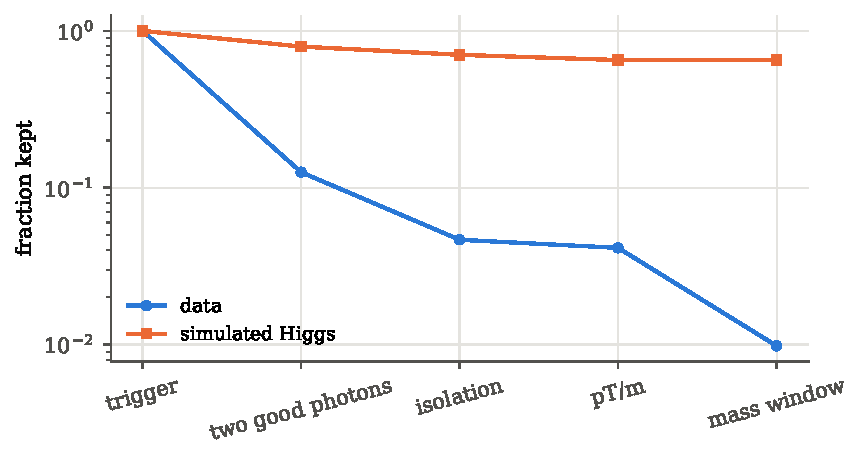
\includegraphics[width=0.82\linewidth]{figures/ch13/hyy_cutflow.pdf}
\caption{The fraction of events kept after each step of the selection, for the recorded
data (blue) and for the simulated Higgs bosons (orange), both relative to the events that
passed the trigger. The photon identification and the isolation remove most of the data and
little of the signal: that is the purpose of each cut. The mass window removes most of the
remaining data, whose spectrum extends far beyond $160\,$GeV.}
\label{13d:fig:cutflow}
\end{figure}

\paragraph{What survives.}
Of $\HyyNTrig$ triggered events, $\HyyNTwo$ have exactly two good photons, $\HyyNIso$ of
these are isolated, $\HyyNKin$ pass the relative momentum cuts and $\HyyNData$ fall in the
mass window (\cref{13d:fig:cutflow}). The four periods contribute $\HyyNA$, $\HyyNB$,
$\HyyNC$ and $\HyyND$ events, in proportion to their luminosity.

\paragraph{How many Higgs bosons should be among them?}
\emph{The question:} the simulation produced about a million ggH events, far more than
the data contain; how does one turn a selected simulated event into a number of expected
real events? If a process has cross section $\sigma$ \unpack{the effective area of the
collision for that process, here including the probability that the Higgs boson decays to
two photons} and the data correspond to an integrated luminosity $L$ \unpack{the number of
collisions per unit area that were recorded}, the expected number of such events produced is
$L\sigma$ (\cref{ch:T4}). The expected number selected is that times the probability
$\varepsilon$ of passing the selection, which the simulation estimates. The simulation's
events carry generator weights $w_j$ (some generators produce weighted, even negatively
weighted, events), and a selected event also carries scale factors $\mathrm{SF}_j$ that
correct the simulated efficiencies of the trigger, the photon identification and the
pile-up to those measured in data. As in \cref{T4a:sec:weights},
\begin{equation}
  S
  \eqby{1} L\,\sigma\,\varepsilon
  \eqby{2} L\,\sigma\,\frac{\sum_{j\in\text{selected}}w_j\,\mathrm{SF}_j}{\sum_{\text{all }j}w_j}
  \eqby{3} \sum_{j\in\text{selected}}\underbrace{\frac{L\,\sigma}{\sum_{\text{all }k}w_k}\,w_j\,\mathrm{SF}_j}_{\text{weight of event }j} .
  \label{13d:eq:mcweight}
\end{equation}
\begin{explain}
  \item Expected selected events: produced events times the selection probability.
  \item The weighted fraction of simulated events that pass; with all weights one it is
        the plain fraction $N_{\rm sel}/N_{\rm gen}$. The sum in the denominator runs over
        all generated events, before any selection, and is stored in the files.
  \item Bring the constant inside the sum: every selected event contributes its own weight.
\end{explain}
With $L=10.06\,\mathrm{fb}^{-1}$ the expected Higgs signal after all cuts is
$S=\HyySigExp$ events: $\HyySigggH$ from gluon fusion, $\HyySigVBF$ from vector-boson fusion,
$\HyySigWH$ and $\HyySigZH$ from production with a $W$ or $Z$. A fraction $\HyyEffSig$ of the
signal events in the files survives the selection (\cref{13d:fig:cutflow}), against
$\HyyNData/\HyyNTrig$ of the data.

\paragraph{The spectrum.}
\Cref{13d:fig:spectrum} shows the $\HyyNData$ masses in $1\,$GeV bins and, below them, the
$\HyySigExp$ expected Higgs events on their own. The data fall smoothly from about
$3000$ to about $600$ events per GeV. The Higgs peak is $60$ to $70$ events per GeV high at
its top, a few per cent of the background there, and no bump is visible by eye: the
error bar of a single bin, $\sqrt{1600}=40$ events, is not much smaller than the whole peak.
Whether the peak is there has to be decided by the likelihood, using all the bins at once.

\begin{figure}[htbp]
\centering
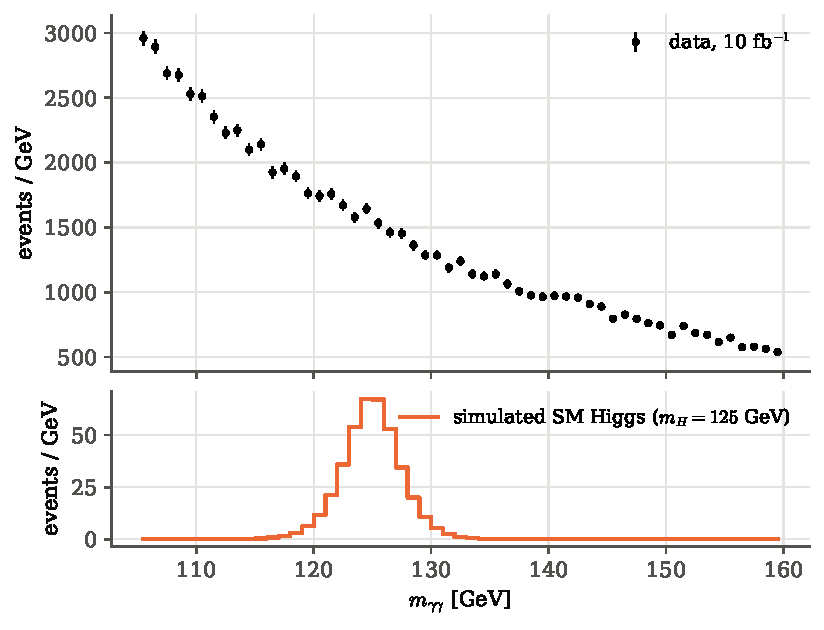
\includegraphics[width=0.85\linewidth]{figures/ch13/hyy_spectrum.pdf}
\caption{Top: the invariant mass of the $\HyyNData$ selected photon pairs in $1\,$GeV bins,
with Poisson error bars. Bottom: the Higgs signal expected in the same data from the
simulation, $\HyySigExp$ events in all, drawn on its own because on the scale of the top
panel it would be a ripple of a few per cent.}
\label{13d:fig:spectrum}
\end{figure}

\paragraph{The full analysis, and ours.}
ATLAS in 2012 split its events into ten categories of different mass resolution and
signal-to-background ratio, fitted each with its own background function, chosen with large
simulated background samples, and combined two collision energies \cite{AadHiggs2012}; the
later analyses of the same detector use many times more data and more categories. We keep
the published selection and one inclusive spectrum, read $1.9\,$GB of files once, and
use two categories only as an illustration (\cref{13d:sec:categories}). The price is
sensitivity, which \cref{13d:sec:repro} quantifies.
\section{Shapes: the Higgs line and the background function}
\label{13d:sec:shapes}

The likelihood of \cref{4b:sec:binned-like} needs two templates: the fraction $f_i$ of the
signal and the fraction $g_i$ of the background expected in each bin $i$ of the mass
histogram, so that the mean count is $\nu_i=\mu Sf_i+Bg_i$ \eqref{4b:eq:nu-template}. In the
pseudo-experiments of \cref{ch:04} both were handed to us. Here the signal template has to
be extracted from the $\HyySigExp$ simulated Higgs events of \cref{13d:sec:data}, and the
background template has to be a smooth function whose parameters are fitted to the data.
Both choices change the answer, and each has its own check.

\subsection{The signal line shape}
\label{13d:sec:signal-shape}

A Higgs boson is so narrow (its natural width is about $4\,$MeV, \cref{ch:T4}) that the
width of the peak in $m_{\gamma\gamma}$ is entirely the detector's: the calorimeter measures
each photon's energy with an error of one or two per cent, and by \eqref{13d:eq:mgg}
$m_{\gamma\gamma}\propto\sqrt{E_1E_2}$ inherits about half of each relative error. Many
small independent errors add up to a Gaussian (the central limit theorem of \cref{ch:02}),
so the core of the peak is Gaussian. But some photons lose part of their energy before they
reach the calorimeter, by converting into an electron--positron pair in the material in
front of it or by leaking out of the back. Such losses only ever lower the measured mass.
The peak therefore has a tail on its low side, and a Gaussian, which is symmetric, misses it.

\paragraph{The Crystal Ball function.}
The standard description, met in \cref{T4a:sec:resolution}, is a Gaussian core glued to a
power-law tail. With
$t=(m-\bar m)/\sigma$ the distance from the peak in units of the core width,
\begin{equation}
  f_{\rm CB}(m)\propto
  \begin{cases}
    e^{-t^2/2}, & t>-\alpha,\\[2pt]
    A\,(B-t)^{-n}, & t\le-\alpha,
  \end{cases}
  \label{13d:eq:cb}
\end{equation}
with four shape parameters: the peak position $\bar m$, the core width $\sigma$, the point
$t=-\alpha$ where the tail takes over, and the power $n$ of the tail. The constants $A$
and $B$ are not free. \emph{The question:} what must they be for the two pieces to join
smoothly at $t=-\alpha$, with the same value and the same slope? Equal slopes first, in
logarithmic form (the log of each piece has a simple derivative):
\begin{align}
  \frac{\dd}{\dd t}\Bigl(-\frac{t^2}{2}\Bigr)\Big|_{t=-\alpha}
  &\eqby{1} \frac{\dd}{\dd t}\bigl(\ln A-n\ln(B-t)\bigr)\Big|_{t=-\alpha}
  \;\Longrightarrow\;
  \alpha=\frac{n}{B+\alpha}
  \;\Longrightarrow\;
  B\eqby{2}\frac{n}{\alpha}-\alpha,
  \nonumber\\
  e^{-\alpha^2/2}
  &\eqby{3} A\,(B+\alpha)^{-n}
  \;\Longrightarrow\;
  A\eqby{4}\Bigl(\frac{n}{\alpha}\Bigr)^{n}e^{-\alpha^2/2}.
  \label{13d:eq:cb-AB}
\end{align}
\begin{explain}
  \item Equal values and equal slopes means equal logarithmic slopes. On the left the
        derivative is $-t=\alpha$; on the right it is $n/(B-t)=n/(B+\alpha)$.
  \item Solve for $B$.
  \item Equal values at $t=-\alpha$.
  \item $B+\alpha=n/\alpha$ by the previous line.
\end{explain}
For the normalisation we need the area of each piece, in units of $\sigma$. The core is a
piece of a Gaussian, $\int_{-\alpha}^{\infty}e^{-t^2/2}\dd t=\sqrt{\pi/2}\,[1+\operatorname{erf}(\alpha/\sqrt2)]$.
The tail is a power law, which integrates in one line:
\begin{align}
  \int_{-\infty}^{-\alpha}A(B-t)^{-n}\dd t
  \eqby{1} A\Bigl[\frac{(B-t)^{1-n}}{n-1}\Bigr]_{-\infty}^{-\alpha}
  \eqby{2} \frac{A}{n-1}\Bigl(\frac{n}{\alpha}\Bigr)^{1-n}
  \eqby{3} \frac{n}{\alpha(n-1)}\,e^{-\alpha^2/2} .
  \label{13d:eq:cb-tail}
\end{align}
\begin{explain}
  \item The antiderivative of $(B-t)^{-n}$ is $(B-t)^{1-n}/(n-1)$; the minus signs from
        the chain rule and from $1-n$ cancel.
  \item For $n>1$ the term at $t\to-\infty$ vanishes; at $t=-\alpha$, $B-t=n/\alpha$.
  \item Insert $A$ from \eqref{13d:eq:cb-AB}: $(n/\alpha)^n(n/\alpha)^{1-n}=n/\alpha$.
\end{explain}
The tail needs $n>1$ to have a finite area at all. As $n\to\infty$ the tail area
$\to e^{-\alpha^2/2}/\alpha$, which is the large-$\alpha$ estimate of the Gaussian's own tail
beyond $-\alpha$ (\cref{ch:04}): a very steep power law is a Gaussian tail again. The
library \pyname{code/ch13/lib_hyy.py} writes the cumulative distribution of
\eqref{13d:eq:cb} from these two areas, so that the expected signal in every bin is an exact
difference of two cumulative values.

\begin{figure}[htbp]
\centering
\begin{tikzpicture}
\begin{axis}[width=10cm,height=5.2cm,xmin=-6,xmax=4,ymin=0.0005,ymax=1.5,ymode=log,
  xlabel={$t=(m-\bar m)/\sigma$},ylabel={density (unnormalised)},
  axis lines=left,tick label style={font=\footnotesize},label style={font=\small},
  legend style={draw=none,font=\footnotesize,at={(0.5,1.03)},anchor=south,legend columns=2},legend cell align=left]
  \addplot[softgray,dashed,thick,domain=-6:4,samples=120] {exp(-x^2/2)};
  \addlegendentry{Gaussian}
  \addplot[formblue,very thick,domain=-1.5:4,samples=80,forget plot] {exp(-x^2/2)};
  \addplot[formblue,very thick,domain=-6:-1.5,samples=80] {2.596*(0.5-x)^(-3)};
  \addlegendentry{Crystal Ball, $\alpha=1.5$, $n=3$}
  \draw[densely dotted,black!60] (axis cs:-1.5,0.0005) -- (axis cs:-1.5,1.5);
  \node[font=\footnotesize,anchor=south east] at (axis cs:-1.55,0.0009) {$t=-\alpha$};
  \node[font=\footnotesize,anchor=west,fibreorange] at (axis cs:-5.8,0.25) {power-law tail};
  \node[font=\footnotesize,anchor=west,formblue] at (axis cs:1.2,0.9) {Gaussian core};
\end{axis}
\end{tikzpicture}
\caption{The Crystal Ball line shape on a logarithmic scale. To the right of $t=-\alpha$ it is
the Gaussian; to the left it continues as a power law that joins with the same value and
slope, \eqref{13d:eq:cb-AB}, and falls far more slowly than the Gaussian (dashed). The
excess area on the left is the events whose photons lost energy before being measured.}
\label{13d:fig:cb}
\end{figure}

\paragraph{Fitting it to the simulation.}
The simulated events carry the weights $w_j$ of \eqref{13d:eq:mcweight}. A weighted
maximum-likelihood fit maximises $\sum_jw_j\ln p(m_j\given\bar m,\sigma,\alpha,n)$, where $p$
is \eqref{13d:eq:cb} normalised over the window $105$--$160\,$GeV: each simulated event
counts as many times as the real events it stands for. The fit to all production modes
together gives
\[
  \bar m=\HyyCBmean\,\text{GeV},\qquad \sigma=\HyyCBsig\,\text{GeV},\qquad
  \alpha=\HyyCBalpha,\qquad n=\HyyCBn,
\]
and a plain Gaussian fitted the same way has width $\HyyGsig\,$GeV (\cref{13d:fig:signal}).
The Gaussian is wider because it has to stretch its symmetric shape to cover the low tail,
which also makes it too wide at the top. The Crystal Ball puts $\HyyTailFrac\%$ of the
signal more than $2\sigma$ below the peak, against $\HyyGaussTail\%$ for a Gaussian. Above
the peak the simulation shows a small tail of its own, which the one-sided function misses;
later analyses use a Crystal Ball with a power law on both sides. Its effect here is a
few events out of $\HyySigExp$.

\paragraph{Example: the full width at half maximum.}
A peak is often quoted by its full width at half maximum (FWHM), because it can be read off
a histogram without a fit. For a Gaussian, half maximum is where $e^{-t^2/2}=\tfrac12$, so
$t=\pm\sqrt{2\ln2}=\pm1.177$ and
\[
  \text{FWHM}=2\sqrt{2\ln2}\,\sigma=2.355\,\sigma .
\]
The Crystal Ball has the same half-maximum points as long as the tail starts beyond them,
$\alpha>1.177$, as it does here. The numerical FWHM of our fit is $\HyyFWHM\,$GeV,
$\HyyFWHMratio\,\sigma$. ATLAS in 2012 quoted a FWHM of $3.9\,$GeV with $\sigma_{\rm CB}=1.6\,$GeV
for its inclusive sample \srcref{AadHiggs2012}{\S5.4}: a ratio of $2.4$, slightly above
$2.355$ because their model adds a wider Gaussian (under $10\%$ of the events) to the
Crystal Ball and the inclusive sample mixes categories of different widths; for single
categories they quote a ratio of typically $2.3$. Their peak was narrower than
ours by a factor $\HyyCBsig/1.6\approx1.5$, a difference we return to in \cref{13d:sec:repro}.

\paragraph{Example: the resolution depends on the photons.}
Fitted separately, the pairs in which both photons are central ($|\eta|<0.75$) and
unconverted have $\sigma=\HyyCBsigCat\,$GeV, the rest $\sigma=\HyyCBsigRest\,$GeV. Central
unconverted photons cross the least material and land in the best part of the calorimeter.
\Cref{13d:sec:categories} uses this difference.

\begin{figure}[htbp]
\centering
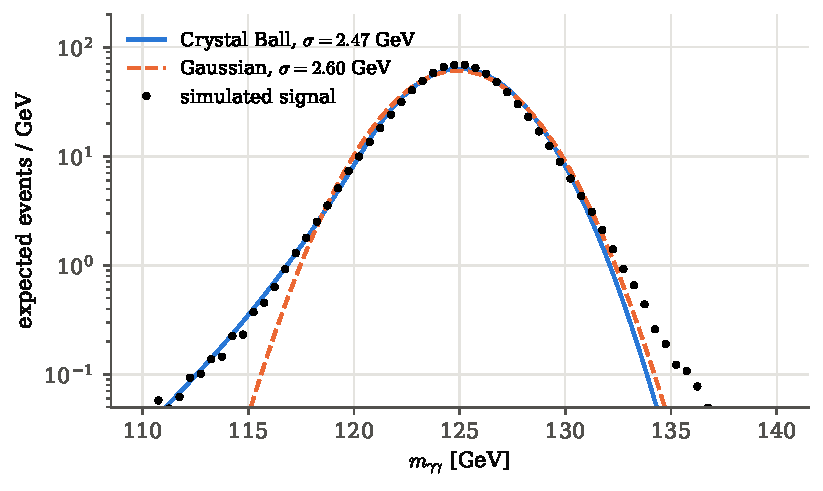
\includegraphics[width=0.85\linewidth]{figures/ch13/hyy_signal_shape.pdf}
\caption{The simulated Higgs signal (points, expected events per GeV for $10\,\mathrm{fb}^{-1}$,
logarithmic scale) with the fitted Crystal Ball (solid) and Gaussian (dashed). The Gaussian
falls far too fast below $118\,$GeV, where the photons that lost energy end up; the Crystal
Ball's power law follows them.}
\label{13d:fig:signal}
\end{figure}

\paragraph{Other masses.}
The search tests masses $m_H$ from $110$ to $150\,$GeV, but the simulation exists only at
$125\,$GeV. The calorimeter's relative resolution changes little over this range, so we
scale both the peak position and the width with the mass,
$\bar m(m_H)=\bar m\,m_H/125$ and $\sigma(m_H)=\sigma\,m_H/125$, and keep $\alpha$ and $n$.
ATLAS interpolates between simulations at several masses \cite{AadHiggs2012}.

\subsection{Choosing the background function: the spurious signal}
\label{13d:sec:spurious}

The background is mostly pairs of real photons from quark--antiquark annihilation and
gluon fusion, plus photon--jet and jet--jet events where a jet passed as a photon
\srcref{AadHiggs2012}{\S5}. No calculation predicts their sum after our cuts to a
fraction of a per cent, which is the precision $\HyyNData$ events demand. So the
background is described by a smooth function with free parameters, fitted to the data
together with the signal. The plain claim is: \emph{any function that fits the data well
will do}. The everyday question behind it is ``does the function fit the data?'', and we
can answer it with the goodness-of-fit test of \cref{4a:sec:gof}.

\paragraph{Does each function fit?}
The script \pyname{code/ch13/32_hyy_model.py} fits eight families to the spectrum with no
signal: exponentials of polynomials of degree one to four (Exp1 to Exp4,
$g(m)\propto\exp\sum_{k=1}^{K}a_ku^k$ with $u$ the mass mapped onto $[-1,1]$), a power law
$m^{-a}$ (Pow) and Bernstein polynomials of degree three to five (Bern3 to Bern5,
$g\propto\sum_{j=0}^{K}c_j\binom Kjx^j(1-x)^{K-j}$ with $x$ the mass mapped onto $[0,1]$).
The deviance $D=2\sum_i[\nu_i-n_i+n_i\ln(n_i/\nu_i)]$ in $1\,$GeV bins is the
likelihood-ratio goodness-of-fit statistic of \cref{4a:sec:gof-fitted}, approximately
$\chi^2$ with $55-1-K$ degrees of freedom.
\begin{center}
\small
\begin{tabular}{@{}lcccccccc@{}}
\toprule
 & Exp1 & Pow & Exp2 & Bern3 & Exp3 & Bern4 & Exp4 & Bern5\\\midrule
free shape parameters $K$ & 1 & 1 & 2 & 3 & 3 & 4 & 4 & 5\\
deviance & $\HyyDevExpOne$ & $\HyyDevPow$ & $\HyyDevExpTwo$ & $\HyyDevBernThree$ & $\HyyDevExpThree$ & $\HyyDevBernFour$ & $\HyyDevExpFour$ & $\HyyDevBernFive$\\
$p$-value & $\HyyPfitExpOne$ & $\HyyPfitPow$ & $\HyyPfitExpTwo$ & $\HyyPfitBernThree$ & $\HyyPfitExpThree$ & $\HyyPfitBernFour$ & $\HyyPfitExpFour$ & $\HyyPfitBernFive$\\
max $|S_{\rm spur}|$ (events) & $\HyySpurExpOne$ & $\HyySpurPow$ & $\HyySpurExpTwo$ & $\HyySpurBernThree$ & $\HyySpurExpThree$ & $\HyySpurBernFour$ & $\HyySpurExpFour$ & $\HyySpurBernFive$\\
max $|S_{\rm spur}|/\sigma_S$ & $\HyySpurRelExpOne$ & $\HyySpurRelPow$ & $\HyySpurRelExpTwo$ & $\HyySpurRelBernThree$ & $\HyySpurRelExpThree$ & $\HyySpurRelBernFour$ & $\HyySpurRelExpFour$ & $\HyySpurRelBernFive$\\
\bottomrule
\end{tabular}
\end{center}
Only the single exponential is rejected at the one-per-cent level. Every other family fits.

\paragraph{The hidden assumption.}
``Fits the data'' answers a question about all $55$ bins at once. The question that matters
for a search is narrower: \emph{if there were no signal at all, would this function, fitted
together with a signal template, return a signal of zero?} A function can follow the data
within the errors everywhere and still be wrong by a few hundred events in a way that looks
like a peak, because a deviation spread over a $6\,$GeV wide region of $\HyyBeta$ background
events per GeV is a fraction of a per cent of the background there, below what the
goodness of fit can see. The test that asks the right question is the
\newterm{spurious-signal} test.

\begin{workdef}[spurious signal]
Take a background spectrum with no signal in it, as realistic as possible (a ``truth'').
Fit it with the candidate background function plus a signal at mass $m_H$. The fitted
signal $S_{\rm spur}(m_H)$ \unpack{events the function invents, or hides when negative}
is the spurious signal. ATLAS required $|S_{\rm spur}|$ below $20\%$ of the statistical
error $\sigma_S$ of the fitted signal at every $m_H$ in $110$--$150\,$GeV
\srcref{AadHiggs2012}{\S5.5}. \emph{Operationally:} fit the truth's exact expectation (an
Asimov spectrum), so that the result is the bias alone, with no fluctuation.
\end{workdef}

\paragraph{Where does a truth come from?}
ATLAS used large samples of simulated background. The open-data release has none for this
selection, so we take as truths the two most flexible families, Bern5 and Exp4, each
fitted to the whole data spectrum \emph{together with} a $125\,$GeV signal, and keep only
their background part. (Fitted without the signal they would have absorbed the real Higgs
boson in the data, which is what we must not call background; their fitted signals were
$\HyyTruthSBernFive$ and $\HyyTruthSExpFour$ events.) Each candidate is then fitted, with a
signal, to each truth's Asimov spectrum scaled to $\HyyNData$ events, at every $m_H$ from
$110$ to $150\,$GeV in $1\,$GeV steps, skipping the truth's own family.

\paragraph{Example: the exponential of a quadratic.}
Exp2 fits the data with $p=\HyyPfitExpTwo$. Against the truths it invents up to
$\HyySpurExpTwo$ events, $\HyySpurRelExpTwo$ times the statistical error $\sigma_S$ of the
signal: a function that passes the goodness-of-fit test would, on a background-only
spectrum, produce a bump of more than two standard deviations by its shape alone.
\Cref{13d:fig:spurious} shows why: its spurious signal oscillates with $m_H$, positive where
the truth bends above the Exp2 shape and negative where it bends below. A rigid function
cannot follow a bend, so it uses the signal template to do it.

\begin{figure}[htbp]
\centering
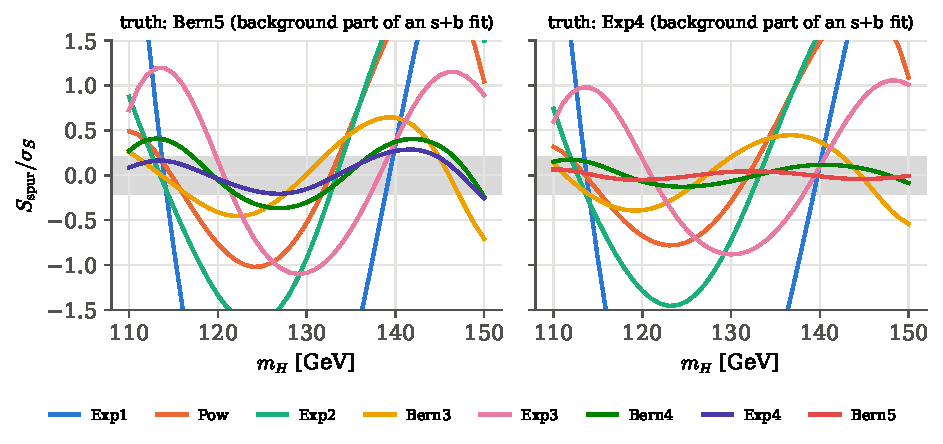
\includegraphics[width=\linewidth]{figures/ch13/hyy_spurious.pdf}
\caption{The spurious signal of each candidate background family, in units of the
statistical error of the fitted signal, against the hypothesised Higgs mass. Left: the
truth is the background part of a Bern5 fit to the data; right: of an Exp4 fit. The grey
band is the $\pm20\%$ criterion. The rigid families (Exp1, Pow, Exp2) swing far outside it;
only the most flexible ones stay close to zero everywhere.}
\label{13d:fig:spurious}
\end{figure}

\paragraph{The verdict, and its limits.}
Only Bern5 passes, with $|S_{\rm spur}|\le\HyySpurBernFive$ events,
$\HyySpurRelBernFive\,\sigma_S$; Bern4 reaches $\HyySpurRelBernFour\,\sigma_S$ against the
Bern5 truth. We use Bern5 from here on. Two honest caveats. The truths are themselves fits
to the same data, so the test checks the families against each other rather than against
an independent truth, and Bern5 has been tested only against Exp4. And with only the data,
a more flexible truth would always make the next family fail. So, as ATLAS did, the
spurious signal also enters the likelihood as a nuisance parameter: a term
$\theta_{\rm ss}S_{\rm spur}f_i(m_H)$ added to the mean, with $S_{\rm spur}=\HyySpurBernFive$
events and a unit Gaussian constraint on $\theta_{\rm ss}$. ``The background model might be
wrong by this much'' becomes a systematic uncertainty of the signal.

\paragraph{The price of flexibility.}
A flexible function invents no signal, but it can also absorb part of a real one: a
fifth-degree polynomial over $55\,$GeV can make a broad wiggle that resembles a
$6\,$GeV-wide peak. How much sensitivity does that cost? \emph{The question in words:} how
much smaller is the expected $q_0$ when the background shape is fitted than when it is
known? By Wald's approximation (\cref{4b:sec:wald-asym}), the expected $q_0$ for a signal
$\mu$ is $q_{0,\rm A}=\mu^2/V_{\mu\mu}$, with $V_{\mu\mu}$ the variance of $\hat\mu$ when the
background parameters are fitted too. With the background known, the variance is the
smaller $1/F_{\mu\mu}$, where $F$ is the Fisher matrix. Then
\begin{equation}
  \frac{q_{0,\rm A}^{\rm fitted}}{q_{0,\rm A}^{\rm known}}
  \eqby{1} \frac{\mu^2/V_{\mu\mu}}{\mu^2F_{\mu\mu}}
  \eqby{2} \frac{1}{F_{\mu\mu}(\Fish^{-1})_{\mu\mu}}
  \eqby{3} 1-\rho^2 ,
  \label{13d:eq:keep}
\end{equation}
\begin{explain}
  \item The Asimov $q_0$ with the profiled and with the conditional variance.
  \item The variance of $\hat\mu$ with all parameters fitted is the $\mu\mu$ element of the
        inverse Fisher matrix (\cref{ch:10}).
  \item The identity $1/F_{\mu\mu}=V_{\mu\mu}(1-\rho^2)$ of \cref{ch:03}, used in
        \eqref{4b:eq:syst}, with $\rho^2$ the fraction of the variance of $\hat\mu$ shared
        with the background parameters.
\end{explain}
The background parameters play exactly the role the systematic uncertainty played in
\eqref{4b:eq:syst}: whatever part of the signal's information they share is lost. On the
Asimov data set of our spectrum with a $\mu=1$ Higgs signal at $125\,$GeV
(\pyname{code/ch13/33_hyy_search.py}):
\begin{center}
\small
\begin{tabular}{@{}lccccccc@{}}
\toprule
background & known & Bern1 & Bern2 & Bern3 & Bern4 & Bern5 & Bern6\\\midrule
expected $Z=\sqrt{q_{0,\rm A}}$ & $\HyyZAknown$ & $\HyyZAdegOne$ & $\HyyZAdegTwo$ & $\HyyZAdegThree$ & $\HyyZAdegFour$ & $\HyyZAdegFive$ & $\HyyZAdegSix$\\
$1-\rho^2$ & $1$ & $\HyyKeepDegOne$ & $\HyyKeepDegTwo$ & $\HyyKeepDegThree$ & $\HyyKeepDegFour$ & $\HyyKeepDegFive$ & $\HyyKeepDegSix$\\
\bottomrule
\end{tabular}
\end{center}
The expected significance falls with every added degree, and the second row explains the
first: each $Z$ is close to the known-background value times $\sqrt{1-\rho^2}$. This is the
trade-off ATLAS describes as a ``compromise between limiting the size of a potential bias
while retaining good statistical power'' \srcref{AadHiggs2012}{\S5.5}: rigid functions bias
the signal, flexible ones dilute it. The narrower the peak, the less a smooth polynomial can
imitate it, which is one reason good mass resolution is worth so much.
\section{Is there a peak? The discovery test}
\label{13d:sec:discovery}

The spectrum of \cref{13d:fig:spectrum} holds $\HyyNData$ photon pairs, and a Standard
Model Higgs boson would add about $\HyySigExp$ of them, piled within a few GeV of
$125\,$GeV. The general problem is old and simple to state: a small number of extra events
is spread over a few bins of a histogram that already contains many events; how should the
counts be combined to decide whether the extra events are there? Before writing the full
likelihood, the smallest version of the problem shows what matters.

\paragraph{The smallest example: one window.}
Count the events in a mass window and compare the count with the background expected in
it. If the window holds $s$ signal and $b$ background events with $b$ large, the count
fluctuates by $\sqrt b$, and the excess is worth about $s/\sqrt b$ standard deviations
(\cref{4b:eq:ZA} with $s\ll b$). The window's width is the only dial, and it acts on both
numbers at once. \emph{The naive choice:} use the whole window $105$--$160\,$GeV, which
certainly contains all the signal. Then $s\approx398$ and $b\approx76\,000$, so
\[
  \frac{s}{\sqrt b}\approx\frac{398}{\sqrt{76\,000}}=\frac{398}{276}=1.44 .
\]
Most of those $76\,000$ events are far from $125\,$GeV and carry no information about the
peak, but each adds its fluctuation. \emph{A better choice:} keep only $m_H\pm k\sigma$
around the peak, with $\sigma=\HyyCBsig\,$GeV the width of the signal from
\cref{13d:sec:signal-shape}. A Gaussian peak puts a fraction $\operatorname{erf}(k/\sqrt2)$ of
its events inside, while the background in the window is its density $\beta$ times the
width $2k\sigma$. Near $125\,$GeV the background density is $\beta=\HyyBeta$ events per
GeV. The ratio $\operatorname{erf}(k/\sqrt2)/\sqrt{2k}$ is largest near $k=1.4$, where the
window keeps $84\%$ of the signal, so
\[
  \frac{s}{\sqrt b}=\frac{0.84\times398}{\sqrt{1527\times2.8\times2.47}}
  =\frac{334}{103}=3.25 .
\]
Cutting away the empty regions more than doubled the significance. \emph{The price:} the
number $b$ under the peak must now be known, and it is not measured inside the window,
where the signal sits; it has to be interpolated from the sidebands with a background
function. Every uncertainty of that interpolation lowers the $3.25$. The lesson in one
line: \emph{the events near the peak carry the information, and the background under the
peak is what we pay to know.} A likelihood does better than any window: it weights every bin by how much signal it can hold, fits the background under the peak
together with the signal, and can ask the discovery question of \cref{4b:sec:limits} at
every mass from $110$ to $150\,$GeV.

\subsection{The likelihood of the spectrum}
\label{13d:sec:likelihood}

\paragraph{The mean count in each bin.}
The histogram now has $220$ bins of $0.25\,$GeV between $105$ and $160\,$GeV, fine enough
that the shape of the peak (about ten bins wide) is not smeared by the binning. Each count
$n_i$ is Poisson, as in \cref{4b:sec:binned-like}, with a mean built from four pieces:
\begin{equation}
  \nu_i
  =\underbrace{\mu\,(1+\delta_y)^{\theta_y}\,s_i(m_H;\theta_\sigma,\theta_m)}_{\text{Higgs signal}}
   +\underbrace{\theta_{\rm ss}\,S_{\rm spur}\,f_i(m_H)}_{\text{spurious signal}}
   +\underbrace{\sum_{j=0}^{5}c_j\,b_{j,5}(m_i)}_{\text{background}} .
  \label{13d:eq:nu}
\end{equation}
Each piece, one at a time:
\begin{itemize}[itemsep=1pt,leftmargin=1.2em]
  \item $s_i(m_H)$ is the number of Higgs events the simulation predicts in bin $i$ for a
        Standard Model Higgs boson of mass $m_H$: the $\HyySigExp$ events of
        \cref{13d:sec:data} distributed with the Crystal Ball shape of
        \eqref{13d:eq:cb}. The \newterm{signal strength} $\mu$ \unpack{the observed signal
        divided by the Standard Model prediction} is the parameter of interest: $\mu=0$
        is no Higgs boson, $\mu=1$ is the Standard Model.
  \item $\theta_y$ moves the expected number of signal events by a relative
        $\delta_y=10\%$ per unit. It stands for everything that scales the signal as a
        whole: the luminosity, the photon identification and isolation efficiencies.
        ATLAS quoted $8$--$11\%$ for the identification and $1.8$--$3.6\%$ for the
        luminosity \srcref{AadHiggs2012}{\S5.6}. The power form $(1+\delta_y)^{\theta_y}$
        keeps the yield positive for any $\theta_y$.
  \item $\theta_\sigma$ changes the width of the peak by a factor
        $(1+\delta_\sigma)^{\theta_\sigma}$ with $\delta_\sigma=14\%$, the resolution
        uncertainty of the 2012 analysis \srcref{AadHiggs2012}{\S5.6}.
  \item $\theta_m$ shifts the peak by a relative $\delta_m\theta_m$, with
        $\delta_m=\HyyRelSyst$, the photon energy-scale uncertainty that the release
        stores for every photon, averaged over the selected signal events (a $1\%$ shift
        of both photon energies moves $m_{\gamma\gamma}\propto\sqrt{E_1E_2}$ by $1\%$).
  \item $\theta_{\rm ss}S_{\rm spur}f_i$ is the spurious signal of
        \cref{13d:sec:spurious}: a signal-shaped term of size $S_{\rm spur}=\HyySpurBernFive$
        events, with $f_i$ the signal shape normalised to one.
  \item $b_{j,5}(m)$ are the six Bernstein basis polynomials of degree five chosen in
        \cref{13d:sec:spurious}, and the $c_j$ are free. They describe the background
        everywhere, under the peak included, without any separate sideband.
\end{itemize}

\paragraph{Constraints.}
The four $\theta$'s are calibrations measured outside this spectrum. As in
\cref{4b:sec:nuisance-hep}, each one comes with an auxiliary measurement $a_k$ whose
likelihood is a Gaussian of unit width, so that $\theta_k=\pm1$ is one standard deviation
of that calibration, and $a_k=0$ for the real data. The whole likelihood is
\eqref{4b:eq:full-like}, and the function we minimise is
\begin{equation}
  -2\ln\Like(\mu,\bm c,\bm\theta)
  =2\sum_{i=1}^{220}\bigl[\nu_i-n_i\ln\nu_i\bigr]+\sum_{k}\bigl(\theta_k-a_k\bigr)^2
   +\text{const},
  \label{13d:eq:nll}
\end{equation}
with eleven parameters: $\mu$, six $c_j$ and four $\theta_k$. The first sum is $-2$ times
the log of the Poisson probabilities, without the $\ln n_i!$ that does not depend on the
parameters; the second is $-2$ times the log of the four Gaussian constraints.
\pyname{code/ch13/lib_hyy.py} codes \eqref{13d:eq:nu} and \eqref{13d:eq:nll} in its class
\pyname{Search} and minimises with MINUIT through \pyname{iminuit}.

\begin{figure}[htbp]
\centering
\begin{tikzpicture}[
  node distance=0.5cm and 0.45cm,
  par/.style={draw=black!50,rounded corners=2pt,font=\footnotesize,align=center,
              inner sep=3pt,fill=formblue!8},
  nuis/.style={par,fill=fibreorange!12},
  aux/.style={draw=black!50,font=\footnotesize,align=center,inner sep=3pt,fill=black!4},
  arr/.style={->,black!60}]
  \node[par] (mu) at (0,0) {$\mu$\\[-1pt]{\scriptsize signal strength}};
  \node[par] (c) at (9.3,0) {$c_0,\dots,c_5$\\[-1pt]{\scriptsize background shape}};
  \node[nuis] (ty) at (1.9,0) {$\theta_y$\\[-1pt]{\scriptsize yield}};
  \node[nuis] (ts) at (3.5,0) {$\theta_\sigma$\\[-1pt]{\scriptsize width}};
  \node[nuis] (tm) at (5.0,0) {$\theta_m$\\[-1pt]{\scriptsize position}};
  \node[nuis] (tss) at (6.6,0) {$\theta_{\rm ss}$\\[-1pt]{\scriptsize spurious}};
  \node[par,fill=black!4,minimum width=10.2cm] (nu) at (4.65,-1.7)
       {$\nu_i$ in each of the $220$ bins, \eqref{13d:eq:nu}};
  \node[aux] (n) at (4.65,-3.0) {counts $n_i$, Poisson with mean $\nu_i$};
  \foreach \a/\l in {1.9/y,3.5/\sigma,5.0/m,6.6/{\rm ss}}
    \node[aux] at (\a,1.35) {$a_{\l}=0$};
  \foreach \a in {1.9,3.5,5.0,6.6}
    \draw[arr] (\a,1.07) -- (\a,0.42);
  \foreach \p in {mu,ty,ts,tm,tss,c} \draw[arr] (\p) -- (\p|-nu.north);
  \draw[arr] (nu) -- (n);
\end{tikzpicture}
\caption{The structure of the diphoton likelihood. The parameter of interest $\mu$ and
the six background coefficients are free; each of the four nuisance parameters (orange)
is tied to an auxiliary measurement $a_k$ by a unit Gaussian. All eleven parameters
together set the mean count of every bin, and the observed counts are Poisson about
those means.}
\label{13d:fig:likelihood}
\end{figure}

\subsection{The scan: local significance}
\label{13d:sec:scan}

\paragraph{The question at one mass.}
Fix a mass, say $m_H=125\,$GeV. \emph{If there were no Higgs boson ($\mu=0$), would an
excess like the one in the data, or a larger one, be something we would reasonably
expect?} The null hypothesis is ``background only'', because its sampling distribution is
the one we can work out: with $\mu=0$, the statistic $q_0$ of \eqref{4b:eq:q0-def} follows
the half-$\chi^2_1$ law of \eqref{4b:eq:F-q0} for a large sample. So the procedure is: fit
\eqref{13d:eq:nll} twice, once with $\mu$ free and once with $\mu=0$, the background and
nuisance parameters re-fitted each time; take $q_0$ as twice the difference of the two
minima of $-\ln\Like$ when $\hat\mu>0$ (and $0$ otherwise); then
\begin{equation}
  p_0=\Prob(q_0\ge q_{0,\rm obs}\given\mu=0)=1-\Phi\bigl(\sqrt{q_{0,\rm obs}}\bigr),
  \qquad
  Z=\Phi^{-1}(1-p_0)=\sqrt{q_{0,\rm obs}},
  \label{13d:eq:p0}
\end{equation}
from \eqref{4b:eq:F-q0} with $\mu'=0$. The significance $Z$ is simply the square root of
$q_0$: that is what makes $q_0$ convenient.

\paragraph{The scan.}
We do not know $m_H$, so \pyname{code/ch13/33_hyy_search.py} repeats the test at every
$m_H$ from $110$ to $150\,$GeV in steps of $0.5\,$GeV. \Cref{13d:fig:p0} shows the
result. The largest excess is at $m_H=\HyyMmax\,$GeV, with
\[
  q_{0,\rm obs}=\HyyQmax,\qquad Z_{\rm loc}=\HyyZloc,\qquad p_{0}=\HyyPloc,\qquad
  \hat\mu=\HyyMuMax .
\]
The word \emph{local} is a warning: this is the p-value of a test made at one mass
chosen in advance, while we chose $\HyyMmax\,$GeV after looking at all of them. The
correction is the subject of \cref{13d:sec:lee}. With all four nuisance parameters held at
their nominal values the largest $Z$ is $\HyyZlocStat$: the calibrations cost almost
nothing here, because a $10\%$ uncertainty on the yield or a $14\%$ uncertainty on the
width changes $q_0$ only at second order when the signal is a small fraction of the
data. Away from the largest excess the two curves of \cref{13d:fig:p0} do separate, most
visibly near $140\,$GeV. There the energy-scale parameter $\theta_m$ can slide the
signal template a few GeV towards the excess at $143\,$GeV, paying for it with its
constraint term $\theta_m^2$. A nuisance parameter that moves the peak competes with the
scanned mass itself; at the top of an excess it has nowhere better to go, which is why the
largest $q_0$ is unchanged. The other excesses in the scan are what background fluctuations look like: the
largest one more than $8\,$GeV away from the peak is at $\HyyMsecond\,$GeV with
$Z=\HyyZsecond$.

\begin{figure}[htbp]
\centering
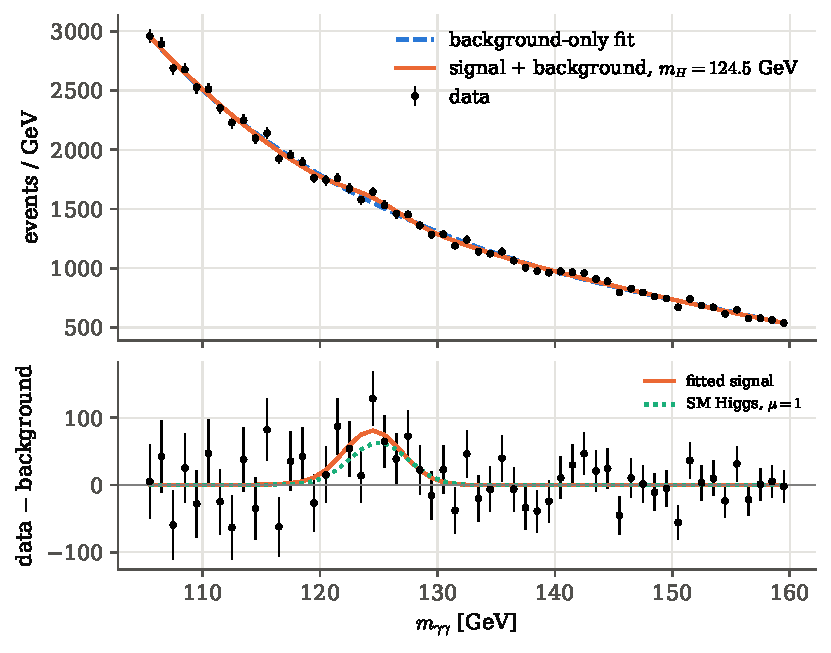
\includegraphics[width=0.85\linewidth]{figures/ch13/hyy_fit.pdf}
\caption{Top: the data in $1\,$GeV bins with the background-only fit (dashed) and the
best signal-plus-background fit at $m_H=\HyyMmax\,$GeV (solid). Bottom: the same data with
the fitted background subtracted. The fitted signal (orange) and the Standard Model
expectation (dotted) are of similar size; the residuals far from the peak scatter about
zero as Poisson noise of about $\pm\sqrt{1600}=\pm40$ events per GeV.}
\label{13d:fig:fit}
\end{figure}

\paragraph{Example: the excess in events.}
At $\HyyMmax\,$GeV the fit gives $\hat\mu=\HyyMuMax$, that is
$\HyyMuMax\times\HyySigExp\approx510$ extra events spread over the peak, against a
background of about $\HyyBeta$ events per GeV. The bottom panel of \cref{13d:fig:fit}
shows them as a bump of about $80$ events per GeV at its top on residuals that scatter by
$\pm40$: a bump no single bin could establish, which the likelihood finds by adding the
evidence of all the bins it covers.

\begin{figure}[htbp]
\centering
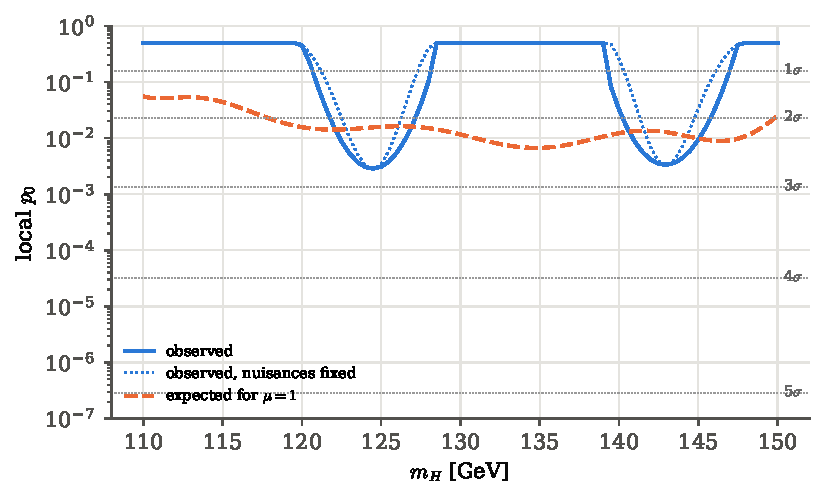
\includegraphics[width=0.85\linewidth]{figures/ch13/hyy_p0.pdf}
\caption{The local p-value $p_0$ of the background-only hypothesis against the tested
mass (solid), with the nuisance parameters fixed at their nominal values (dotted) and the
median expected for a Standard Model Higgs boson at each mass (dashed, from Asimov data
sets). The horizontal lines mark $1\sigma$ to $5\sigma$. The observed curve dips where
the data have an excess, and the expected curve says how deep the dip should be if the
Standard Model Higgs boson were at that mass.}
\label{13d:fig:p0}
\end{figure}

\subsection{How large an excess should we expect?}
\label{13d:sec:expected}

\paragraph{The question.}
A local $Z$ of $\HyyZloc$ is neither a discovery nor nothing. To judge it we need to know
what a Standard Model Higgs boson would typically produce in this data set. \emph{If the
truth were $\mu=1$ at $125\,$GeV, what $q_0$ would we typically see?} The answer is the
Asimov data set of \cref{4b:sec:asimov}: replace the counts by their expected values
$n_i=b_i+s_i$, with $b_i$ the fitted background, and compute $q_0$ on them. By
\eqref{4b:eq:asimov-med} the result $q_{0,\rm A}$ is the median of $q_0$ under $\mu=1$, so
$\sqrt{q_{0,\rm A}}$ is the median significance. The script does this at each mass, which
gives the dashed curve of \cref{13d:fig:p0}; at $125\,$GeV,
\[
  Z_{\rm exp}=\sqrt{q_{0,\rm A}}=\HyyZexpOneTwoFive .
\]
The data show $\HyyZoneTwoFive$ at $125\,$GeV, and $\hat\mu=\HyyMuMax$ at the peak: a
little more signal than the Standard Model predicts, within the fluctuations
\cref{13d:sec:measure} quantifies.

\paragraph{Where the expected significance comes from.}
\emph{The question:} which features of the data set the number $\HyyZexpOneTwoFive$? Start
from the simplest case, the background known exactly and no nuisance parameters. The
bins are independent, so $\ln\Like$ is a sum over bins and so is $q_0$. In each bin the
Asimov value is the counting result \eqref{4b:eq:ZA}. With $x_i=s_i/b_i$, which is below
$0.1$ in every bin,
\begin{align}
  q_{0,\rm A}
  &\eqby{1} 2\sum_i\Bigl[(s_i+b_i)\ln\Bigl(1+\frac{s_i}{b_i}\Bigr)-s_i\Bigr]
   \eqby{2} 2\sum_i\Bigl[b_i(1+x_i)\Bigl(x_i-\frac{x_i^2}{2}+\frac{x_i^3}{3}-\cdots\Bigr)-b_ix_i\Bigr]
  \nonumber\\
  &\eqby{3} 2\sum_i b_i\Bigl[\frac{x_i^2}{2}-\frac{x_i^3}{6}+\cdots\Bigr]
   \relby{4}{\approx} \sum_i\frac{s_i^2}{b_i} .
  \label{13d:eq:s2b}
\end{align}
\begin{explain}
  \item \eqref{4b:eq:ZA} applied bin by bin and summed, since $q_0$ is a sum of
        independent bins when the background is known.
  \item Write $s_i=b_ix_i$ and expand $\ln(1+x)=x-x^2/2+x^3/3-\cdots$.
  \item Multiply out: $(1+x)(x-x^2/2+x^3/3)=x+x^2/2-x^3/6+\cdots$, and the leading $x$
        cancels against $-b_ix_i$.
  \item Keep the first term, $b_ix_i^2=s_i^2/b_i$; the next is smaller by a factor $x_i/3$.
\end{explain}
Each bin contributes the square of its own counting significance $s_i/\sqrt{b_i}$, and
squares add. This is the window of the opening example with every bin given its own
weight: a bin with no signal contributes nothing (instead of adding noise), and the bins at
the top of the peak contribute most. On our spectrum $\sqrt{\sum_is_i^2/b_i}=\HyyZsumsb$.

\paragraph{The same in closed form.}
A peak of $S$ events with a Gaussian shape of width $\sigma$, on a background of density
$\beta$ events per GeV that is nearly flat across it, has $s_i=S\,\varphi(m_i)\,\Delta$ and
$b_i=\beta\Delta$ in bins of width $\Delta$, with $\varphi$ the Gaussian density. For
bins much narrower than $\sigma$ the sum becomes an integral:
\begin{align}
  q_{0,\rm A}
  &\eqby{1} \sum_i\frac{S^2\varphi(m_i)^2\Delta^2}{\beta\Delta}
   \eqby{2} \frac{S^2}{\beta}\int\varphi(m)^2\,\dd m
   \eqby{3} \frac{S^2}{\beta}\cdot\frac{1}{2\pi\sigma^2}\int e^{-(m-m_H)^2/\sigma^2}\dd m
  \nonumber\\
  &\eqby{4} \frac{S^2}{\beta}\cdot\frac{\sqrt\pi\,\sigma}{2\pi\sigma^2}
   = \frac{S^2}{2\sqrt\pi\,\sigma\,\beta} .
  \label{13d:eq:zgauss}
\end{align}
\begin{explain}
  \item Insert $s_i$ and $b_i$ into \eqref{13d:eq:s2b}.
  \item One factor $\Delta$ is left: $\sum_i g(m_i)\Delta\to\int g\,\dd m$.
  \item The square of $\varphi(m)=e^{-(m-m_H)^2/2\sigma^2}/(\sqrt{2\pi}\sigma)$.
  \item The Gaussian integral $\int e^{-u^2/a^2}\dd u=\sqrt\pi\,a$ with $a=\sigma$.
\end{explain}
\Cref{13d:eq:zgauss} says the peak acts like a counting window of effective width
$2\sqrt\pi\,\sigma=3.54\,\sigma$ holding all $S$ events: $Z^2=S^2/(\beta\times3.54\sigma)$.
It shows the three dials of every resonance search at once. The significance grows like
the signal $S$, falls like the square root of the background density, and falls like the
square root of the mass resolution. Halving $\sigma$ is worth as much as halving the background density $\beta$:
either one doubles $Z^2$.

\paragraph{Example: our numbers.}
With $S=\HyySwin$ events in the window, $\sigma=\HyyCBsig\,$GeV and $\beta=\HyyBeta$ per
GeV,
\[
  q_{0,\rm A}\approx\frac{398^2}{2\times1.772\times2.467\times1527}
  =\frac{158\,400}{13\,350}=11.9,\qquad Z\approx3.44,
\]
the value $\HyyZgaussForm$ printed by the script, against $\HyyZsumsb$ from the exact sum
with the Crystal Ball shape. The tail of the Crystal Ball puts a few per cent of the
signal where the background is large, which costs a little.

\paragraph{From $3.4$ to $\HyyZexpOneTwoFive$: what the fit costs.}
The full Asimov value at $125\,$GeV is $\HyyZexpOneTwoFive$, well below $\HyyZsumsb$. The
difference is the price paid at the end of the opening example: the background under the
peak is not known but fitted. By \eqref{13d:eq:keep}, fitting six background coefficients
together with $\mu$ keeps a fraction $1-\rho^2=\HyyKeepDegFive$ of $q_{0,\rm A}$, and
\[
  \HyyZsumsb\times\sqrt{\HyyKeepDegFive}\approx\HyyZAdegFive ,
\]
the expected significance with the degree-five background in the table of
\cref{13d:sec:spurious}. The nuisance parameters take the rest of the way to
$\HyyZexpOneTwoFive$. So most of the loss is the background function, and very little is
the calibrations. A real analysis fights this loss by splitting the events into
categories with different $\sigma$ and $\beta$ (\cref{13d:sec:categories}) and by using a
background function no more flexible than the spurious-signal test demands.

\begin{pitfall}
$Z_{\rm exp}$ is the \emph{median} significance under $\mu=1$, not a prediction of what
this data set will show. The observed $q_0$ fluctuates about $q_{0,\rm A}$ with a spread of
about $2\sqrt{q_{0,\rm A}}$ (\cref{4b:eq:wald}: $\sqrt{q_0}=\hat\mu/\sigma_\mu$ is Gaussian
with unit width), so with $Z_{\rm exp}=\HyyZexpOneTwoFive$ a true Standard Model Higgs
boson gives $Z$ anywhere between about $1.2$ and $3.2$ in two thirds of repetitions.
\end{pitfall}
\section{Anywhere in the range: checking the formulas and looking elsewhere}
\label{13d:sec:lee}

Two claims of \cref{13d:sec:discovery} rest on formulas rather than on the data. The
local p-value $\HyyPloc$ came from the half-$\chi^2$ law \eqref{4b:eq:F-q0}, which Wald's
approximation guarantees only for a large sample and a well-behaved fit, and here the fit
has eleven parameters and a background that bends. And the excess at $\HyyMmax\,$GeV was
picked as the largest of $81$ tested masses, so its local p-value is not the probability
that background alone produces such an excess \emph{somewhere}. Both are questions about
the sampling distribution of $q_0$ under the background-only hypothesis, and both can be
answered by simulating the experiment many times.

\paragraph{What we saw in the toy bump hunt, and what is different now.}
In \cref{4b:sec:scan} a simulated spectrum of $\FourBScBtot$ events with a known
exponential background was scanned for a Gaussian peak of width $\FourBScSigM\,$GeV over
$50\,$GeV. Its largest bump had $Z_{\rm loc}=\FourBScZloc$; $\FourBScToys$
background-only scans made that a global $\FourBScZglob\sigma$, a trials factor of
$\FourBScTrials$, and the Gross--Vitells formula \eqref{4b:eq:gv}, calibrated on $100$
scans, reproduced it. The method is the same now. Three things differ, and each changes
the size of the correction. The peak is wider, $\sigma=\HyyCBsig\,$GeV against
$\FourBScSigM$, and the range is shorter, $40\,$GeV against $50$: there are fewer
independent places for a fluctuation to appear, roughly $40/2.5=16$ against $50/1.5=33$.
The background shape is fitted in every toy, with six coefficients, so a toy that
fluctuates in a smooth, broad way is absorbed by the background rather than counted as a
bump. And the local significance is lower, $\HyyZloc$ against $\FourBScZloc$, and by
\eqref{4b:eq:trials} the trials factor grows with the local significance. All three
point to a smaller trials factor than the $\FourBScTrials$ of the toy.

\paragraph{How the toys are made.}
\pyname{code/ch13/34_hyy_toys.py} draws each background-only toy as $220$ Poisson counts
whose means are the background-only fit to the data, $b_i$. Every toy is then analysed
exactly as the data: the degree-five Bernstein background is refitted, and $q_0$ is
computed at all $81$ masses. Fitting $81$ masses for each of thousands of spectra with
MINUIT would take hours, but the model with the four nuisance parameters fixed is linear
in its seven free parameters ($\mu$ and the six $c_j$). For a mean linear in the
parameters, $\ln\Like=\sum_i(n_i\ln\nu_i-\nu_i)$ is concave, so Newton's method converges
from any reasonable start, and it can be run on $250$ spectra at once as matrix
operations. At the largest excess the nuisance parameters changed $Z$ by less than $0.01$
(\cref{13d:sec:scan}), and the largest $q_0$ of a scan is what the global p-value
counts, so fixing them in the toys leaves it unchanged. Scanned with
this fitter, the data give $q_{0,\rm obs}=\HyyToyQobs$ at $\HyyToyMobs\,$GeV, essentially
the $\HyyQmax$ of the full fit.

\subsection{Is the half-$\chi^2$ law right?}
\label{13d:sec:asym-check}

\emph{The question:} if there were no Higgs boson, how would $q_0$ at one fixed mass,
$125\,$GeV, be distributed over repetitions of the experiment? The half-$\chi^2$ law
makes three checkable predictions. Half of the toys should have $\hat\mu\le0$ and so
$q_0=0$ exactly; the toys give $\HyyToyFracZero$. The fraction with $q_0>4$ (a local
$2\sigma$) should be $\Phi(-2)=\HyyToyPfourTh$; the toys give $\HyyToyPfour$. The fraction
with $q_0>9$ (a local $3\sigma$) should be $\Phi(-3)=\HyyToyPnineTh$; the toys give
$\HyyToyPnine$. With $\HyyToyNbkg$ toys the statistical error of a fraction $p$ is
$\sqrt{p(1-p)/\HyyToyNbkg}$, about $0.002$ at $0.023$ and $0.0006$ at $0.0013$, so the
agreement is as good as the toys can tell. \Cref{13d:fig:toys} (left, blue) shows the whole
tail.

The same question under the signal hypothesis tells us whether the Asimov expected
significance is the median, as \eqref{4b:eq:asimov-med} says. Toys drawn with
$\mu=1$ at $125\,$GeV have a median $\sqrt{q_0}$ of $\HyyToyZmedSb$, against the Asimov
value $\HyyToyZAsb$, and the central $68\%$ lie between $\HyyToyZsbLo$ and $\HyyToyZsbHi$:
a spread of one unit in $Z$, as the pitfall of \cref{13d:sec:expected} said. Only a
fraction $\HyyToyPsbFive$ of experiments of this size would see a Standard Model Higgs
boson at $5\sigma$. With $76\,000$ events the asymptotic formulas are doing exactly what
they promise; they were derived for this situation.

\begin{figure}[htbp]
\centering
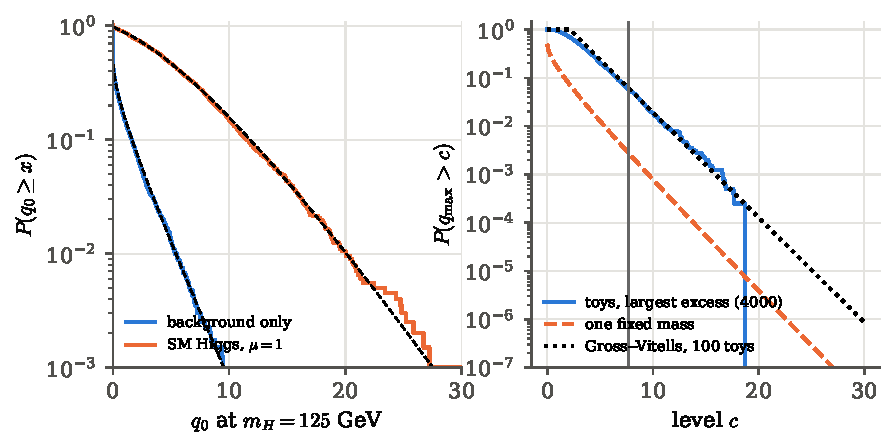
\includegraphics[width=\linewidth]{figures/ch13/hyy_toys_q0.pdf}
\caption{Left: the probability that $q_0$ at $125\,$GeV exceeds $x$, from toys with
background only (blue) and with a Standard Model Higgs boson (orange), against the
asymptotic formulas (black dashed). The step at $x=0$ in the blue curve is the half of
the toys with $\hat\mu\le0$. Right: the probability that the largest $q_0$ anywhere in
$110$--$150\,$GeV exceeds a level $c$ (blue, $\HyyToyNbkg$ toys), the probability at one
fixed mass (orange dashed), and the Gross--Vitells formula calibrated on the first $100$
toys (black dotted). The vertical line is the excess in the data.}
\label{13d:fig:toys}
\end{figure}

\subsection{The global p-value}
\label{13d:sec:global}

\paragraph{The question.}
\emph{If there were no Higgs boson, how often would an excess as large as the one we saw
appear somewhere between $110$ and $150\,$GeV?} The event is now ``the largest $q_0$ in
the scan is at least $q_{0,\rm obs}=\HyyToyQobs$''. Each toy gives one largest $q_0$, so
the answer is a count: $\HyyToyNexceed$ of the $\HyyToyNbkg$ background-only toys have
$q_{\max}\ge\HyyToyQobs$, so
\[
  p_{\rm glob}=\HyyToyPglob\pm\HyyToyPglobErr ,
\]
with the binomial error $\sqrt{p(1-p)/N}$ of \cref{ch:04}.

\paragraph{The same from a hundred toys.}
For a stronger excess the counting would need millions of toys. The Gross--Vitells
formula \eqref{4b:eq:gv} needs only the mean number of upcrossings of a low level, which a
few scans measure well. Counting how often each of the first $100$ toy scans crosses
$c_0=0.5$ upwards gives $\E[N(c_0)]=\HyyENhundred$ (all $\HyyToyNbkg$ toys:
$\HyyENall$). Then, at $c=q_{0,\rm obs}$,
\begin{align}
  p_{\rm glob}
  &\eqby{1} p_{\rm loc}(c)+\E[N(c_0)]\,e^{-(c-c_0)/2}
   \eqby{2} \Phi\bigl(-\sqrt{\HyyToyQobs}\bigr)+\HyyENhundred\,e^{-(\HyyToyQobs-0.5)/2}
  \nonumber\\
  &\eqby{3} \HyyPgvObs ,
  \qquad Z_{\rm glob}=\HyyZgvObs .
  \label{13d:eq:gv-data}
\end{align}
\begin{explain}
  \item The Gross--Vitells formula \eqref{4b:eq:gv}: the chance of being above $c$ at the
        start of the range plus the expected number of upward crossings of $c$, scaled
        down from the reference level $c_0$ by $e^{-(c-c_0)/2}$.
  \item Insert the observed $q_0$ and the measured $\E[N(c_0)]$.
  \item Evaluate, and convert to a significance with $Z=\Phi^{-1}(1-p)$.
\end{explain}
The two routes agree within the error of the toy count, and the right panel of
\cref{13d:fig:toys} shows that they agree over the whole curve, not only at the observed
value. With the full likelihood (all nuisance parameters free) the local significance is
$\HyyZlocFull$, and the same formula gives $Z_{\rm glob}=\HyyZgvFull$.

\paragraph{The trials factor.}
The ratio of the two p-values is $p_{\rm glob}/p_{\rm loc}=\HyyTrialsObs$. Its asymptotic
form \eqref{4b:eq:trials}, $1+\sqrt{2\pi}\,\mathcal N_1Z$ with
$\mathcal N_1=\E[N(c_0)]e^{c_0/2}=\HyyNone$, gives $\HyyTrialsAsym$. Both are below the
$\FourBScTrials$ of the toy bump hunt, for the three reasons met there: a wider peak and a shorter range, a
fitted background and a lower local significance. The number $\mathcal N_1=\HyyNone$, against $\FourBScNone$ in \cref{4b:sec:scan},
measures how many independent places the scan offers. It is smaller, as expected, but
not half as small as the crude count of range over width ($16$ against $33$) suggested:
that count is only a rough guide, and the upcrossings measure the real number directly.

\paragraph{Example: how often background alone gives a local $3\sigma$ somewhere.}
At a fixed mass a local $3\sigma$ excess has probability $0.0013$. Somewhere in the range
it is far more common: the toys give $\HyyPthreeGlobToy$ and the formula
$\HyyPthreeGlobGV$, so roughly one search in thirty of this size shows a
local $3\sigma$ bump with no Higgs boson at all. That is why particle physics asks
for $5\sigma$ before it says ``discovery'': a $3\sigma$ excess in a scan is a reason to
look again with more data, not a result.

\paragraph{The data's second bump.}
The scan of \cref{13d:fig:p0} has a second excess, at $\HyyMsecond\,$GeV with local
$Z=\HyyZsecond$, almost as large as the one at the Higgs mass. Nothing is expected there,
and the global p-value is exactly the tool that tells us not to be impressed: an excess of
that size somewhere in the range happens in about $\HyyToyPglob$ of background-only
experiments. The data alone cannot say which of the two bumps is the Higgs boson. What
singles out $125\,$GeV is outside this spectrum: the 2012 discovery in this and other decay
channels, and the expected size of the signal.

\paragraph{Which range?}
The global p-value depends on the range searched, and the range has to be fixed before
the data are seen. In 2012 ATLAS quoted both: a global $5.1\sigma$ for
$110$--$600\,$GeV and $5.3\sigma$ for $110$--$150\,$GeV, from a local $5.9\sigma$ in all
channels combined \srcref{AadHiggs2012}{\S9}. For us, in 2016 data, the mass was already
known to a fraction of a GeV, and the honest test is the local one at $125\,$GeV:
$Z=\HyyZoneTwoFive$. Had we searched only $120$--$130\,$GeV, the expected number of
upcrossings would be a quarter of that for $40\,$GeV, and the formula gives
$Z_{\rm glob}=\HyyZgvNarrow$.

\begin{inpractice}[Toys in a real analysis]
The LHC experiments compute local significances with the asymptotic formulas, check them
with toys at a few masses as above, and quote global significances from the
Gross--Vitells formula or a variant with several search dimensions (mass and width)
\cite{GrossVitells2010,Cowan2011}. Toys are run in full only where the formulas are in
doubt: few events, a parameter near a boundary, or a statistic far in its tail. Each toy
there is a full fit with every nuisance parameter, and the auxiliary measurements $a_k$
are drawn afresh in each toy, which our statistics-only toys skip.
\end{inpractice}
\section{How strong, and where? Measuring $\mu$ and $m_H$}
\label{13d:sec:measure}

Once a signal is taken to be present, the question changes from ``is it there?'' to ``how
much of it is there, and where?''. The first is a test with one answer, yes or no at a
chosen level; the second is a measurement with an interval. The data are the same
$\HyyNData$ masses, the likelihood is the same \eqref{13d:eq:nll}, and the tool is the
profile likelihood ratio $\lambda(\mu)$ of \eqref{4b:eq:lambda} read as a curve rather
than at one point.

\subsection{The signal strength}
\label{13d:sec:mu}

\paragraph{The question.}
\emph{Which values of $\mu$ at $m_H=125\,$GeV are compatible with the data?} For each
trial $\mu$ we fit everything else (the six background coefficients and the four
nuisance parameters) and record how much worse the best fit is than the overall best:
$-2\ln\lambda(\mu)$. By Wald's approximation \eqref{4b:eq:wald},
$-2\ln\lambda(\mu)\approx(\mu-\hat\mu)^2/\sigma_\mu^2$, a parabola that reaches $1$ at
$\hat\mu\pm\sigma_\mu$. So the values where the curve crosses $1$ bound the $68\%$
interval, and this remains true when the curve is not a parabola, because a
reparametrisation that would make it one does not move the crossing points
(\cref{4b:sec:likelihood-interval}).

\paragraph{The result.}
\Cref{13d:fig:mu-mass} (left) shows the curve. It crosses $1$ at
\[
  \hat\mu=\HyyMuHat\,^{+\HyyMuHi}_{-\HyyMuLo}\qquad(m_H=125\,\text{GeV}).
\]
The Standard Model value $\mu=1$ lies inside; $\mu=0$, no Higgs boson, is at
$-2\ln\lambda=\HyyZoneTwoFive^2\approx7.5$, which is the $q_0$ of \cref{13d:sec:scan}
read from the other side. The interval is wider above than below. The yield enters as
$\mu(1+\delta_y)^{\theta_y}$, so the uncertainty it carries is a fixed fraction of $\mu$:
for large $\mu$ it is larger in absolute terms.

\paragraph{How much of it is statistics?}
Repeating the scan with the four nuisance parameters fixed at their nominal values gives
the dashed curve, crossing $1$ at $\pm\HyySigStat$. That is the uncertainty we would have
with perfect calibrations: the statistical part. If the statistical and the systematic
fluctuations of $\hat\mu$ are independent and Gaussian, their variances add, and the
systematic part follows by subtraction:
\begin{equation}
  \sigma_{\rm tot}^2\eqby{1}\sigma_{\rm stat}^2+\sigma_{\rm syst}^2
  \quad\Longrightarrow\quad
  \sigma_{\rm syst}\eqby{2}\sqrt{\sigma_{\rm tot}^2-\sigma_{\rm stat}^2}
  =\sqrt{0.52^2-0.46^2}\approx\HyySigSyst .
  \label{13d:eq:syst}
\end{equation}
\begin{explain}
  \item The variance of a sum of independent fluctuations is the sum of their variances.
  \item Solve for the systematic part, with $\sigma_{\rm tot}=\HyySigTot$ the half-width of
        the total interval.
\end{explain}
So $\hat\mu=\HyyMuHat\pm\HyySigStat\,(\text{stat})\pm\HyySigSyst\,(\text{syst})$. A $10\%$ yield
uncertainty alone would give $0.10\times\HyyMuHat\approx0.13$; the width and the position
of the peak add the rest, because a wider or shifted template changes how many events the
fit assigns to the peak. Statistics dominate: this measurement would improve with more
data long before better calibrations mattered.

\paragraph{What the nuisance parameters did.}
At the best fit the four nuisance parameters sit at $\hat\theta_y=0.00$ and
$\hat\theta_{\rm ss}=0.00$ (to two decimals), $\hat\theta_\sigma=\HyyThSig$ and
$\hat\theta_m=\HyyThM$, all well within one standard deviation of their calibrations. The data cannot distinguish
a larger yield from a larger $\mu$, so they leave $\theta_y$ where its constraint puts it.
Only $\theta_m$ moves: the data's peak sits a little below the simulated one. A nuisance
parameter that the fit pushes far from zero would be a sign that a calibration and the
data disagree, and would have to be investigated before quoting anything.

\paragraph{Example: compared with the Standard Model and with 2012.}
Our $\hat\mu=\HyyMuHat\pm\HyySigTot$ differs from the Standard Model value by
$(\HyyMuHat-1)/\HyySigTot\approx0.5$ standard deviations. ATLAS measured
$\hat\mu=1.8\pm0.5$ in the diphoton channel in 2012 \srcref{AadHiggs2012}{Table~7}, a
value $1.6$ standard deviations above one. The two results differ by
$(1.8-\HyyMuHat)/\sqrt{0.5^2+\HyySigTot^2}\approx0.7$ standard deviations: entirely
compatible. The high 2012 value was partly the luck of the experiment that made the
discovery: a search that happens to fluctuate upwards is the one that crosses $5\sigma$
first.

\subsection{The mass}
\label{13d:sec:mass}

\paragraph{The question.}
\emph{Which Higgs masses are compatible with the data?} The same recipe applies with $m_H$
in the place of $\mu$: for each trial $m_H$ from $120$ to $130\,$GeV, fit everything else,
$\mu$ included, and plot $-2\ln\lambda(m_H)$ (\cref{13d:fig:mu-mass}, right). It crosses
$1$ at
\[
  \hat m_H=\HyyMhat\pm\HyyMhatLo\,\text{GeV}
  \quad\text{(all nuisances)},\qquad
  \hat m_H=\HyyMhatStat\,^{+\HyyMhatStatHi}_{-\HyyMhatStatLo}\,\text{GeV}
  \quad\text{(nuisances fixed)}.
\]
Here the systematic part is larger than for $\mu$. The photon energy scale is known to
$\delta_m=\HyyRelSyst$, which at $125\,$GeV is $\pm1.07\,$GeV, and a shift of the energy
scale moves the peak exactly as a shift of $m_H$ does, so the data cannot separate them.
In quadrature, $\sqrt{0.85^2+1.07^2}=1.37$, the total.

\paragraph{How precisely should a peak locate a mass?}
The statistical $\pm0.85\,$GeV is far smaller than the width $\sigma=\HyyCBsig\,$GeV of the
peak. \emph{The question:} how does the position error depend on the peak? The Fisher
information on the position $m_0$ of a peak with $s_i=S\varphi(m_i-m_0)\Delta$ on a flat
background $b_i=\beta\Delta$ is $\sum_i(\partial s_i/\partial m_0)^2/b_i$, the same kind of
sum as \eqref{13d:eq:s2b} with the derivative of the signal in the place of the signal
(\cref{ch:10}). For a Gaussian peak, $\partial\varphi/\partial m_0=\bigl((m-m_0)/\sigma^2\bigr)\varphi$:
\begin{align}
  \frac{1}{\sigma_m^2}
  &\eqby{1} \frac{S^2}{\beta}\int\frac{(m-m_0)^2}{\sigma^4}\,\varphi(m-m_0)^2\,\dd m
   \eqby{2} \frac{S^2}{\beta}\cdot\frac{1}{2\pi\sigma^6}\int u^2e^{-u^2/\sigma^2}\dd u
  \nonumber\\
  &\eqby{3} \frac{S^2}{\beta}\cdot\frac{1}{2\pi\sigma^6}\cdot\frac{\sqrt\pi\,\sigma^3}{2}
   = \frac{S^2}{4\sqrt\pi\,\sigma^3\beta}
   \eqby{4} \frac{q_{0,\rm A}}{2\sigma^2} .
  \label{13d:eq:sigma-m}
\end{align}
\begin{explain}
  \item The sum over narrow bins becomes an integral, as in \eqref{13d:eq:zgauss}.
  \item Write $u=m-m_0$ and square
        $\varphi=e^{-u^2/2\sigma^2}/(\sqrt{2\pi}\sigma)$.
  \item The second moment of a Gaussian: $\int u^2e^{-u^2/a^2}\dd u=\sqrt\pi\,a^3/2$ with
        $a=\sigma$.
  \item Compare with $q_{0,\rm A}=S^2/(2\sqrt\pi\sigma\beta)$ of \eqref{13d:eq:zgauss}.
\end{explain}
So $\sigma_m=\sqrt2\,\sigma/Z$, with $Z=\sqrt{q_{0,\rm A}}$ the significance of the peak: a
peak located to a fraction of its width, and the fraction is $\sqrt2$ over its
significance. A barely significant peak locates nothing; a $5\sigma$ peak locates its mass
to $0.28$ of its width. For the signal the data show, $\hat\mu=\HyyMuHat$ times the
known-background $Z=\HyyZAknown$, this gives
$\sqrt2\times\HyyCBsig/(\HyyMuHat\times\HyyZAknown)\approx0.80\,$GeV, close to the
$\pm0.85$ of the profile. (The fitted background costs little here: a smooth polynomial
cannot imitate the antisymmetric change that shifting a peak makes.)

\paragraph{Example: the 2012 mass.}
For the diphoton channel in 2012, $\sigma_{\rm CB}=1.6\,$GeV and a local $Z=4.5$
\srcref{AadHiggs2012}{Table~7} give $\sigma_m\approx\sqrt2\times1.6/4.5=0.50\,$GeV; the
statistical error ATLAS quoted for the combined mass, dominated by the diphoton and
four-lepton channels, was $0.4\,$GeV \srcref{AadHiggs2012}{\S9}. Their peak was narrower
and more significant, so their statistical error was smaller than our $\pm0.85\,$GeV
by almost a factor of two.

\begin{figure}[htbp]
\centering
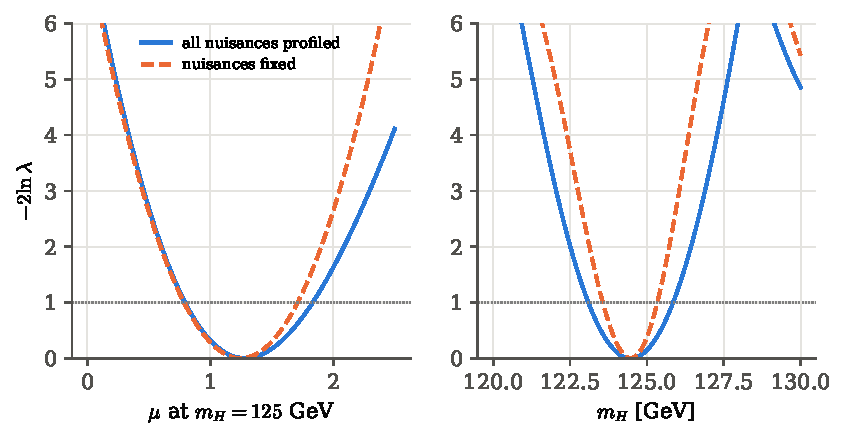
\includegraphics[width=\linewidth]{figures/ch13/hyy_mu_mass.pdf}
\caption{Left: $-2\ln\lambda$ as a function of the signal strength at $m_H=125\,$GeV,
with all nuisance parameters profiled (solid) and fixed (dashed). The crossings of the
dotted line at $1$ bound the $68\%$ intervals. Right: the same for the Higgs mass. The
solid curve is much wider than the dashed one for the mass, because the photon energy
scale shifts the peak exactly as a different mass would; for $\mu$ the two curves are
close, because the measurement is limited by statistics.}
\label{13d:fig:mu-mass}
\end{figure}

\subsection{Splitting the events into categories}
\label{13d:sec:categories}

The opening example of \cref{13d:sec:discovery} showed that bins with more signal per
background carry more information. The same holds for groups of events. In
\cref{13d:sec:signal-shape} the pairs with both photons central and unconverted had a
narrower peak, $\sigma=\HyyCBsigCat\,$GeV, than the rest, $\sigma=\HyyCBsigRest\,$GeV. If we
fit the two groups as separate spectra, each with its own background, the narrow peak is
no longer diluted by the wide one.

\paragraph{Why splitting cannot hurt.}
\emph{The question:} if two independent spectra share one $\mu$, how do their
significances combine? The likelihood is the product of the two (the rule by which Junk
combined the LEP search channels \cite[(1)]{Junk1999}), so $\ln\Like$ and $q_0$
are sums, and \eqref{13d:eq:s2b} becomes a sum over categories $c$ and their bins. Take
two categories with $S_1$, $S_2$ signal and $B_1$, $B_2$ background in comparable windows.
Split, $Z^2=S_1^2/B_1+S_2^2/B_2$; merged, $Z^2=(S_1+S_2)^2/(B_1+B_2)$. Their difference is
\begin{align}
  \frac{S_1^2}{B_1}+\frac{S_2^2}{B_2}-\frac{(S_1+S_2)^2}{B_1+B_2}
  &\eqby{1} \frac{S_1^2B_2(B_1+B_2)+S_2^2B_1(B_1+B_2)-(S_1+S_2)^2B_1B_2}{B_1B_2(B_1+B_2)}
  \nonumber\\
  &\eqby{2} \frac{S_1^2B_2^2-2S_1S_2B_1B_2+S_2^2B_1^2}{B_1B_2(B_1+B_2)}
   \eqby{3} \frac{(S_1B_2-S_2B_1)^2}{B_1B_2(B_1+B_2)}\ \ge 0 .
  \label{13d:eq:split}
\end{align}
\begin{explain}
  \item Bring the three terms to the common denominator $B_1B_2(B_1+B_2)$.
  \item Expand: the terms $S_1^2B_1B_2$ and $S_2^2B_1B_2$ cancel against those of
        $-(S_1^2+2S_1S_2+S_2^2)B_1B_2$.
  \item A perfect square.
\end{explain}
Splitting gains exactly when the categories have different signal-to-background ratios,
$S_1/B_1\ne S_2/B_2$, and never loses (as long as the background in each category is
determined as well as before, which with fitted backgrounds is only approximately true).

\paragraph{Example: two categories in our data.}
The central unconverted category holds $\HyyNcat$ events and $\HyyScat$ expected Higgs
events with $\sigma=\HyyCBsigCat\,$GeV; the rest holds $\HyyNrest$ events and $\HyySrest$
Higgs events with $\sigma=\HyyCBsigRest\,$GeV. Near $125\,$GeV the fitted background densities are about $\beta_1\approx171$ and
$\beta_2\approx1360$ events per GeV (the signal yields $\HyyScat$ and $\HyySrest$ divided by
$\beta$ are $\HyySbCat$ and $\HyySbRest\,$GeV). With
\eqref{13d:eq:zgauss} for each,
\[
  Z_1^2=\frac{58.8^2}{2\times1.772\times1.825\times171}=3.1,\qquad
  Z_2^2=\frac{339.1^2}{2\times1.772\times2.58\times1360}=9.2,
\]
so $Z=\sqrt{12.4}=3.52$ split, against $3.44$ merged. The full fit with fitted backgrounds
(statistical part only) gives an expected $\HyyZAcat$ split against $\HyyZAincl$ merged,
and on the data $\HyyZOcat$ against $\HyyZOincl$, with $\hat\mu=\HyyMuOcat$ against
$\HyyMuOincl$ (\cref{13d:fig:categories}). The gain is small because only one Higgs event
in seven lands in the good category. ATLAS in 2012 used ten categories built from the
photon positions, conversions and the transverse momentum of the pair, and
\cref{13d:sec:repro} shows what that bought.

\begin{figure}[htbp]
\centering
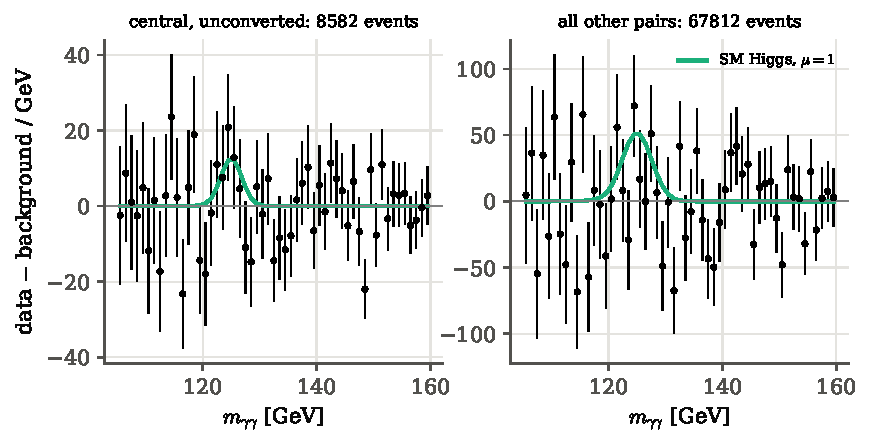
\includegraphics[width=\linewidth]{figures/ch13/hyy_categories.pdf}
\caption{The data minus the fitted background in the two categories, with the
Standard Model Higgs signal expected in each (orange). The central unconverted pairs (left)
are fewer, but their peak is narrower and stands higher above the noise relative to its
size; the rest (right) holds most of the signal on a much larger background.}
\label{13d:fig:categories}
\end{figure}
\section{Where can a Higgs boson be excluded?}
\label{13d:sec:limits}

Before July 2012 the main output of every Higgs search was not a significance but a list
of excluded masses. By then the searches at LEP, the Tevatron and the first LHC data had
excluded a Standard Model Higgs boson at $95\%$ confidence everywhere below $600\,$GeV
except for some regions between $116$ and $127\,$GeV \srcref{AadHiggs2012}{\S1}. An
exclusion answers the opposite question to a discovery. The hypothesis under test is now
the signal: \emph{if a Higgs boson with strength $\mu$ existed at mass $m_H$, would data as
background-like as ours, or more so, be something we would reasonably expect?} If not,
that $\mu$ is excluded at that mass.

\paragraph{What we saw in \cref{ch:04}, and what is new.}
In \cref{4b:sec:fc-poisson} the question was asked of a single count, with
$\mathrm{CL}_{s+b}$ and $\mathrm{CL}_s$ computed from Poisson sums. In
\cref{4b:sec:cls-hep,4b:sec:brazil} the same ideas were carried to a binned likelihood
with nuisance parameters: the statistic $\tilde q_\mu$ \eqref{4b:eq:qtilde}, its
asymptotic distribution \eqref{4b:eq:F-qtilde}, the CL$_s$ upper limit
\eqref{4b:eq:cls-up} and the expected band \eqref{4b:eq:band}, all computed on a simulated
spectrum. The formulas are the same now. What is new is a scan of $41$ masses on real
data, where the observed limit can be compared with what the experiment should have
achieved, and a check of the asymptotic CL$_s$ limit against toys.

\paragraph{The statistic and the two p-values.}
At each mass $m_H$ and each trial $\mu$ the script computes $\tilde q_\mu$ from two fits of
\eqref{13d:eq:nll}: with $\mu$ fixed and with $\mu$ free (or at $0$ if the free fit gives
$\hat\mu<0$). It is large when the data have too few events for a signal of strength
$\mu$, and zero when they have more than $\mu$ predicts, because an upper limit should not
be strengthened by an excess. Two p-values follow from the observed value, one under each
hypothesis:
\begin{itemize}[itemsep=1pt,leftmargin=1.2em]
  \item $\mathrm{CL}_{s+b}=\Prob(\tilde q_\mu\ge\tilde q_{\mu,\rm obs}\given\mu)$: how often
        a world with the signal gives data at least this background-like;
  \item $\mathrm{CL}_b=\Prob(\tilde q_\mu\ge\tilde q_{\mu,\rm obs}\given0)$: how often a
        world without it does.
\end{itemize}
Both come from \eqref{4b:eq:F-qtilde}, with $\mu'=\mu$ and $\mu'=0$. Excluding $\mu$
whenever $\mathrm{CL}_{s+b}<0.05$ would be a valid test, but it has a flaw that Read
described with two experiments \cite{Read2002}: when the background fluctuates down, an
experiment can exclude signals so small that it could never have seen them, and an
experiment with more background can then quote the stronger limit. The CL$_s$ method
divides by $\mathrm{CL}_b$,
\begin{equation}
  \mathrm{CL}_s=\frac{\mathrm{CL}_{s+b}}{\mathrm{CL}_b}<\alpha=0.05 ,
  \label{13d:eq:cls}
\end{equation}
which leaves the test unchanged where the two hypotheses predict very different data
($\mathrm{CL}_b\approx1$) and makes exclusion harder where they predict nearly the same
data ($\mathrm{CL}_b$ small) \cite{Junk1999,Read2002}. The price is over-coverage: a
true signal is excluded in fewer than $5\%$ of experiments, as \cref{4b:fig:fc-coverage}
showed for counts.

\paragraph{The one number the formulas need.}
The asymptotic distributions contain one unknown, the standard deviation $\sigma$ of
$\hat\mu$. \emph{The question:} how is it found without simulation? By
\eqref{4b:eq:asimov-med}, with the background-only Asimov data set ($n_i=b_i$, the true
$\mu'=0$), $\sigma_{\rm A}^2=\mu^2/\tilde q_{\mu,\rm A}$: fit the expected background
spectrum with $\mu$ fixed, see how much worse it fits than with $\mu$ free, and read off
the width. Because $\sigma$ depends a little on $\mu$ (the nuisance parameters scale
with the signal), the script computes it at $\mu=0.25$, $0.5$, $1$ and $2$ and
interpolates. At $125\,$GeV, $\sigma_{\rm A}=\HyySigmaAOneTwoFive$ at $\mu=1$; the
statistical-only estimate of \cref{13d:sec:mu} was $\HyySigStat$, and the difference is
the systematic part. The observed limit $\mu_{\rm up}$ is then the $\mu$ at which
\eqref{13d:eq:cls} becomes an equality, found by root finding.

\paragraph{What should we have excluded?}
An observed limit means little without the limit the experiment expected. \emph{The
question:} if there is no Higgs boson at this mass, what limit would the experiment
typically report, and in what range? Without signal, $\hat\mu\sim\Normal(0,\sigma^2)$,
and the CL$_s$ limit is an increasing function of $\hat\mu$; so its quantiles are the
limits at the quantiles of $\hat\mu$, which is \eqref{4b:eq:band}:
\[
  \mu_{\rm up}(N)=\sigma_{\rm A}\bigl[N+\Phi^{-1}\bigl(1-\alpha\,\Phi(N)\bigr)\bigr],
  \qquad N=-2,-1,0,1,2 .
\]
The median $N=0$ gives $\sigma_{\rm A}\Phi^{-1}(1-\alpha/2)=1.96\,\sigma_{\rm A}$. At
$140\,$GeV, $\sigma_{\rm A}=\HyySigmaAOneFourty$ and the expected median limit is
$\HyyLimExpOneFourty=\HyyBandCoefMed\,\sigma_{\rm A}$, the small difference from $1.96$
coming from the change of $\sigma_{\rm A}$ with $\mu$.

\paragraph{Example: the $+1\sigma$ edge of the band.}
For $N=1$: $\Phi(1)=0.841$, so $1-0.05\times0.841=0.958$ and $\Phi^{-1}(0.958)=1.73$. The
edge is at $\sigma_{\rm A}(1+1.73)=2.73\,\sigma_{\rm A}$, which at $140\,$GeV is
about $2.73\times0.477=1.30$. Without the division by $\mathrm{CL}_b$ the edge would be at
$\sigma_{\rm A}(1+1.645)=2.65\,\sigma_{\rm A}$: when the data fluctuate up, CL$_s$ and
CL$_{s+b}$ differ little. For $N=-2$ the difference is large. $\Phi(-2)=0.0228$, so
$\Phi^{-1}(1-0.05\times0.0228)=\Phi^{-1}(0.99886)=3.05$ and the edge is at
$1.05\,\sigma_{\rm A}$, where CL$_{s+b}$ alone would give $(-2+1.645)\sigma_{\rm A}<0$,
an exclusion of every signal including zero. That negative limit is exactly what CL$_s$
was built to forbid.

\begin{figure}[htbp]
\centering
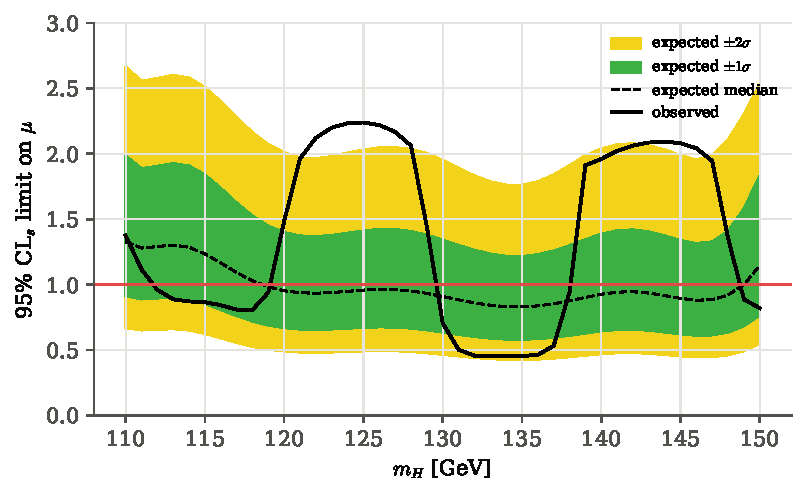
\includegraphics[width=0.85\linewidth]{figures/ch13/hyy_brazil.pdf}
\caption{The $95\%$ CL$_s$ upper limit on the signal strength $\mu$ against the Higgs mass.
The dashed line is the median expected without a Higgs boson, the green and yellow bands
the ranges expected in $68\%$ and $95\%$ of background-only experiments, and the solid
line the observed limit. Where the solid line is below the red line at $\mu=1$, a Higgs
boson with the expected signal is excluded. The observed limit leaves the band upwards
near $125\,$GeV, where the data contain the Higgs boson, and near $143\,$GeV, where they
contain a fluctuation.}
\label{13d:fig:brazil}
\end{figure}

\paragraph{The result.}
\Cref{13d:fig:brazil} shows the observed limit and the expected band from $110$ to
$150\,$GeV. The median expected limit lies between $\HyyLimExpMin$ and $\HyyLimExpMax$,
highest at the low end of the range, where the background is largest, and at the edges
of the fitted window, where the polynomial background is most flexible. So with $10\,$fb$^{-1}$
at $13\,$TeV the diphoton channel alone expects to exclude a Higgs boson of the Standard
Model size over most of the range, but only barely: the median is close to one. The
observed limit excludes $\mu=1$ at $\HyyNexcl$ of the $\HyyNmlim$ masses, in the ranges
\HyyExclRanges\,GeV, and leaves a gap around $125\,$GeV where the observed limit,
$\HyyLimObsOneTwoFive$, is more than twice the expected $\HyyLimExpOneTwoFive$. That gap is
the excess of \cref{13d:sec:discovery} seen from the other side: a limit cannot exclude a
signal that is there. The other gap, near $143\,$GeV, is the second bump of
\cref{13d:sec:global}; there the observed limit at $140\,$GeV is $\HyyLimObsOneFourty$
against an expected $\HyyLimExpOneFourty$. A limit curve on real data is read with the
p-value scan beside it: the first says what the data rule out, the second what they
might contain.

\paragraph{What ``$\mu=1$ at another mass'' means here.}
The simulation exists only at $125\,$GeV, so at every mass we used the same expected yield,
$\HyySigExp$ events, with the shape scaled as in \cref{13d:sec:signal-shape}. The true
Standard Model yield changes with mass: above about $130\,$GeV both the production cross
section and the diphoton branching ratio fall. Our $\mu$ away from $125\,$GeV is therefore
measured relative to a signal of the $125\,$GeV size, not to the Standard Model at that
mass; ATLAS used simulations at many masses \srcref{AadHiggs2012}{\S5.4} and expected to
exclude $110$--$140\,$GeV in 2012, observing $112$--$123$ and $132$--$143\,$GeV
\srcref{AadHiggs2012}{Table~7}. The pattern is the same as ours: an exclusion on both
sides of the peak and a hole where the boson is.

\subsection{Are the asymptotic limits right?}
\label{13d:sec:cls-toys}

\emph{The question:} does the CL$_s$ computed from the half-$\chi^2$-type formulas agree
with CL$_s$ computed from the actual distribution of $\tilde q_\mu$? At $140\,$GeV,
\pyname{code/ch13/34_hyy_toys.py} draws $\HyyNlimToys$ spectra with signal strength $\mu$
and $\HyyNlimToys$ with background only, for each $\mu$ on a grid, computes $\tilde q_\mu$
for each with the background refitted, and counts the fractions above the observed value:
those fractions are $\mathrm{CL}_{s+b}$ and $\mathrm{CL}_b$ directly
\cite[(3)--(6)]{Junk1999}. (These toys hold the four nuisance parameters fixed, as in
\cref{13d:sec:lee}; the statistical-only $\sigma_{\rm A}$ at $140\,$GeV is
$\HyySigAstatOneFourty$.)

\Cref{13d:fig:toys-qtilde} (left) compares the two distributions of $\tilde q_\mu$ for
$\mu=\HyyQtMuTest$ with the asymptotic curves of \eqref{4b:eq:F-qtilde}: under the signal
hypothesis the half-$\chi^2$ for small values and a shifted Gaussian tail for large ones,
under background only a distribution pushed to larger values. The toys follow the curves.
The right panel shows CL$_s$ as a function of $\mu$; the toy points scatter about the
asymptotic line, and the $95\%$ limits are
\[
  \mu_{\rm up}^{\rm toys}=\HyyLimToyOneFourty,\qquad
  \mu_{\rm up}^{\rm asymptotic}=\HyyLimAsymOneFourty .
\]
The two agree to within the scatter of the toy points. Both are about half the limit
$\HyyLimObsOneFourty$ that the full likelihood gives at the same mass. That difference is
not an error of the formulas but the energy-scale parameter: with $\theta_m$ free, a
signal hypothesised at $140\,$GeV can slide towards the excess at $143\,$GeV
(\cref{13d:sec:scan}), so the data look less background-like for it and its exclusion is
weaker. A comparison of toys with asymptotics must use one and the same likelihood, as it
does here. With $76\,000$ events, about $1500$ per GeV under the peak, the asymptotic
formulas are accurate to the precision a few thousand toys can measure. They would not be for a
search with a handful of events in the signal region, which is where the toy method of
\cite{Junk1999,Read2002} came from: the LEP Higgs searches, with a few candidates each.

\begin{figure}[htbp]
\centering
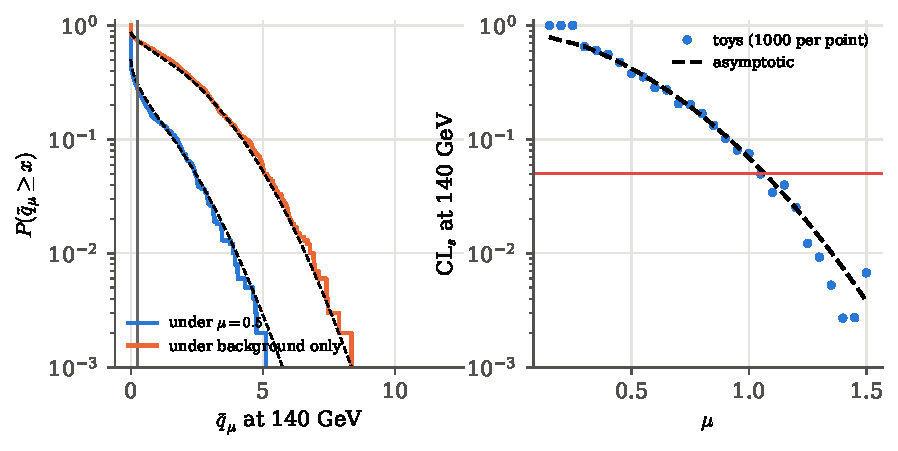
\includegraphics[width=\linewidth]{figures/ch13/hyy_toys_qtilde.pdf}
\caption{Left: the distribution of $\tilde q_\mu$ at $140\,$GeV for $\mu=\HyyQtMuTest$, from
toys with that signal (blue) and with background only (orange), against the asymptotic
formulas (black dashed); the vertical line is the value in the data. Right: CL$_s$ against
$\mu$ from the toys (points, $\HyyNlimToys$ toys per hypothesis and $\mu$) and from the
asymptotic formulas (dashed); the limit is where they cross $0.05$ (red line).}
\label{13d:fig:toys-qtilde}
\end{figure}
\section{Reproducing the 2012 diphoton result}
\label{13d:sec:repro}

The 2012 ATLAS paper has met us before. In \cref{T4a:sec:higgs-counts} its Table 4 gave
the number of expected diphoton events, and from $N_S=110.5$, $\sigma\times\mathrm{BR}=50\,$fb
and $L=5.9\,\mathrm{fb}^{-1}$ we recomputed a selection efficiency of $0.375$ at $8\,$TeV;
\cref{T4a:sec:local-global} went through its local and global significances; and
\cref{T4a:sec:higgs-lesson} noted that the open-data files store a gluon-fusion
$\sigma\times\mathrm{BR}(\gamma\gamma)$ twice as large as the 2012 value. Those were counts of
events. The same table now answers a different question, how significant those events
were expected to be, and it lets us set the 2012 result and ours side by side ingredient by
ingredient. The efficiency below combines both collision energies, so it differs slightly
from the $8\,$TeV value.

\subsection{Their question}
\label{13d:sec:repro-question}

In the first half of 2012 the Higgs boson was the last missing particle of the Standard
Model, and only a narrow window of masses near $125\,$GeV had not yet been excluded
(\cref{13d:sec:limits}). ATLAS asked whether the diphoton spectrum, combined over the
2011 data at $7\,$TeV and the first 2012 data at $8\,$TeV, showed a peak in that window
that the background could not explain, and if so how strong it was
\cite{AadHiggs2012}. Their answer in the diphoton channel alone was a local excess of
$4.5\sigma$ at $126.5\,$GeV where $2.5\sigma$ was expected, with
$\hat\mu=1.8\pm0.5$ \srcref{AadHiggs2012}{Table~7}. Ours, from $10\,\mathrm{fb}^{-1}$ of
2016 data at $13\,$TeV, is $\HyyZoneTwoFive\sigma$ at $125\,$GeV where $\HyyZexpOneTwoFive$
was expected, with $\hat\mu=\HyyMuHat\pm\HyySigTot$. \emph{Why did a search with about the
same luminosity, at a higher energy where the Higgs boson is produced more than twice as
often, expect less?} The answer is in the ingredients, and one formula can compare them.

\subsection{Their setup}
\label{13d:sec:repro-setup}

The 2012 analysis used $4.8\,\mathrm{fb}^{-1}$ at $7\,$TeV and $5.9\,\mathrm{fb}^{-1}$ at
$8\,$TeV. The photon selection is close to ours (two isolated photons, relative momentum
cuts of $0.35$ and $0.25$), with a fit range of $100$--$160\,$GeV. The essential
difference is that the events were split into ten categories, by where the photons hit
the calorimeter (central, rest, the transition region), whether they converted, the
transverse momentum $p_{Tt}$ of the pair relative to its thrust axis, and a category with
two forward jets for vector-boson fusion \srcref{AadHiggs2012}{\S5.3}. For each
category they published three numbers per collision energy in their Table 4: the number of
data events $N_D$ in $100$--$160\,$GeV, the expected number of signal events $N_S$ at
$m_H=126.5\,$GeV, and the full width at half maximum of the signal. Their sums are:
\begin{center}
\small
\begin{tabular}{@{}lccc@{}}
\toprule
 & $7\,$TeV & $8\,$TeV & together\\\midrule
luminosity ($\mathrm{fb}^{-1}$) & $4.8$ & $5.9$ & $10.7$\\
$\sigma\times\mathrm{BR}(H\to\gamma\gamma)$ (fb) & $39$ & $50$ & \\
data events $N_D$, $100$--$160\,$GeV & $23\,788$ & $35\,251$ & $\HyyAtlasND$\\
expected signal $N_S$ & $79.6$ & $110.5$ & $\HyyAtlasS$\\
FWHM, inclusive (GeV) & \multicolumn{2}{c}{$3.9$} & $\sigma\approx\HyyAtlasSigma$\\
\bottomrule
\end{tabular}
\end{center}
The background in each category was a fourth-order Bernstein polynomial, an exponential of
a second-order polynomial or an exponential, chosen by the spurious-signal test of
\cref{13d:sec:spurious} \srcref{AadHiggs2012}{\S5.5}.

\subsection{Their key equation, derived}
\label{13d:sec:repro-equation}

ATLAS computed their expected significance $E(Z_l)$ from Asimov data sets with the full
likelihood. With only Table 4 in hand we cannot redo that, but everything needed for the
leading-order expected significance is there. \emph{The question:} what expected
significance do the published numbers imply? Three results already derived combine into
one formula:
\begin{enumerate}[label=\arabic*.]
  \item a Gaussian peak of $S$ events and width $\sigma$ on a background of density
        $\beta$ per GeV has $q_{0,\rm A}=S^2/(2\sqrt\pi\,\sigma\beta)$,
        \eqref{13d:eq:zgauss};
  \item independent categories (and independent collision energies) add their
        $q_{0,\rm A}$, \cref{13d:sec:categories};
  \item fitting the background shape keeps a fraction $1-\rho^2$ of it,
        \eqref{13d:eq:keep}.
\end{enumerate}
So
\begin{equation}
  Z_{\rm exp}^2\approx(1-\rho^2)\sum_{c}\frac{S_c^2}{2\sqrt\pi\,\sigma_c\,\beta_c},
  \qquad
  \sigma_c=\frac{\mathrm{FWHM}_c}{2\sqrt{2\ln2}},
  \label{13d:eq:repro}
\end{equation}
with the sum over the ten categories at each energy, twenty terms in all.

\paragraph{The symbol map.}
Their $N_S$ is our $S_c$. Their FWHM becomes our $\sigma_c$ through the Gaussian relation of
\cref{13d:sec:signal-shape}; we use it for both energies, since Table 4 gives it only at
$8\,$TeV. Their $N_D$ counts events in the whole $60\,$GeV window, while $\beta_c$ is the
density \emph{under the peak}. \emph{How do we get one from the other?} The spectrum falls
roughly exponentially, by a factor of about $3.9$ from $100$ to $160\,$GeV in their
Fig.~4, so its decay length is $\lambda=60/\ln3.9\approx\HyyAtlasLam\,$GeV. For an
exponential the ratio of the density at the peak, $26.5\,$GeV into the window, to the
mean density is
\begin{align}
  \frac{\beta(126.5)}{N_D/60}
  &\eqby{1} \frac{e^{-26.5/\lambda}}{\frac{1}{60}\int_0^{60}e^{-x/\lambda}\dd x}
   \eqby{2} \frac{60\,e^{-26.5/\lambda}}{\lambda\,(1-e^{-60/\lambda})}
   \eqby{3} \frac{60\times0.548}{44\times0.744}=1.00 .
  \label{13d:eq:beta-atlas}
\end{align}
\begin{explain}
  \item Density at $x=26.5\,$GeV over the mean density of the window, both for
        $e^{-x/\lambda}$; the normalisation cancels.
  \item The integral of an exponential.
  \item $e^{-26.5/44}=0.548$ and $1-e^{-60/44}=1-1/3.9=0.744$.
\end{explain}
The peak happens to sit where the density equals the window's mean, so
$\beta_c=N_{D,c}/60\,$GeV to within a per cent. Finally their $E(Z_l)$ is our
$Z_{\rm exp}=\sqrt{q_{0,\rm A}}$, and their $\mu$ is ours.

\paragraph{The background factor.}
The last ingredient, $1-\rho^2$, depends on the background function and the window. The
script computes it from the Fisher matrix \eqref{13d:eq:keep} for a Gaussian peak of the
inclusive width on an exponential background: for their fourth-order Bernstein polynomial
over $60\,$GeV it is $\HyyAtlasKeep$, and for our fifth-order one over $55\,$GeV with our
wider peak, $\HyyOurKeepGauss$. A narrower peak is harder for a polynomial to imitate, so
it loses less.

\subsection{What we compute}
\label{13d:sec:repro-compute}

\pyname{code/ch13/35_hyy_atlas2012.py} types in Table 4, evaluates each of the twenty
terms of \eqref{13d:eq:repro} and the inclusive version (one category with the totals),
and evaluates the same formula on our spectrum with $S=\HyySwin$, the FWHM of our fitted
Crystal Ball, $\HyyOurFWHM\,$GeV, and $\beta=\HyyBeta$ per GeV. It also reads the cross
section times branching ratio stored in our four simulation files, to separate the
signal per $\mathrm{fb}^{-1}$ into ``how many Higgs bosons decayed to two photons'' and
``what fraction of them we selected''.

\subsection{Side by side}
\label{13d:sec:repro-side}

\begin{center}
\small
\begin{tabular}{@{}lcc@{}}
\toprule
 & ATLAS 2012 ($7+8\,$TeV) & open data ($13\,$TeV)\\\midrule
luminosity ($\mathrm{fb}^{-1}$) & $10.7$ & $10.06$\\
$\sigma\times\mathrm{BR}(H\to\gamma\gamma)$ (fb) & $39$, $50$ & $\HyyOurXS$\\
Higgs bosons to $\gamma\gamma$ produced & $\HyyAtlasProduced$ & $\HyyOurProduced$\\
selection efficiency & $\HyyAtlasEff$ & $\HyyOurEff$\\
expected signal $S$ per $\mathrm{fb}^{-1}$ & $\HyyAtlasSperL$ & $\HyyOurSperL$\\
background under the peak, per GeV per $\mathrm{fb}^{-1}$ & $\HyyAtlasBetaPerL$ & $\HyyOurBetaPerL$\\
mass resolution $\sigma$ (GeV) & $\HyyAtlasSigma$ & $\HyyCBsig$\\
categories & $10$ per energy & $1$\\
$1-\rho^2$ of the background fit & $\HyyAtlasKeep$ & $\HyyOurKeepGauss$\\\midrule
$Z_{\rm exp}$, formula, inclusive, $1-\rho^2=1$ & $\HyyAtlasZincl$ & $\HyyOurZformula$\\
$Z_{\rm exp}$, formula, categories, $1-\rho^2=1$ & $\HyyAtlasZcat$ & \\
$Z_{\rm exp}$, formula with $1-\rho^2$ & $\HyyAtlasZpred$ & $\HyyOurZpred$\\
$Z_{\rm exp}$, full Asimov fit & $2.5$ (quoted) & $\HyyZexpOneTwoFive$\\
$Z_{\rm obs}$ (local) & $4.5$ & $\HyyZoneTwoFive$\\
$\hat\mu$ & $1.8\pm0.5$ & $\HyyMuHat\pm\HyySigTot$\\
\bottomrule
\end{tabular}
\end{center}

\paragraph{The expected significance.}
From nothing but Table 4, \eqref{13d:eq:repro} gives $\HyyAtlasZpred$ for ATLAS against
the $2.5$ they quoted, and $\HyyOurZpred$ for us against our full Asimov value
$\HyyZexpOneTwoFive$. The leading-order formula with the background factor captures what
the full likelihood does to within a few per cent. The comparison of the two
``inclusive'' entries, $\HyyAtlasZincl$ against $\HyyAtlasZcat$, shows what the ten
categories were worth to ATLAS; for us, two categories gained only from $\HyyZAincl$ to
$\HyyZAcat$ (\cref{13d:sec:categories}).

\paragraph{Growth with luminosity.}
At a fixed analysis, $S$ and $\beta$ both grow in proportion to the luminosity $L$, so by
\eqref{13d:eq:zgauss} $Z_{\rm exp}\propto S/\sqrt{\beta}\propto\sqrt L$. A $5\sigma$
expected significance needs $L(5/Z_{\rm exp})^2$: $\HyyAtlasLumiForFive\,\mathrm{fb}^{-1}$
with the 2012 diphoton analysis, $\HyyLumiForFive\,\mathrm{fb}^{-1}$ with ours.
\Cref{13d:fig:atlas2012} shows both lines with the two observations. ATLAS did not wait for
$43\,\mathrm{fb}^{-1}$: the discovery came from combining the diphoton excess with the
four-lepton and $WW$ channels, $5.9\sigma$ locally from $4.9\sigma$ expected
\srcref{AadHiggs2012}{Table~7}, and from an upward fluctuation that made the diphoton
excess $\HyyAtlasMuPull$ standard deviations larger than the Standard Model predicted.

\begin{figure}[htbp]
\centering
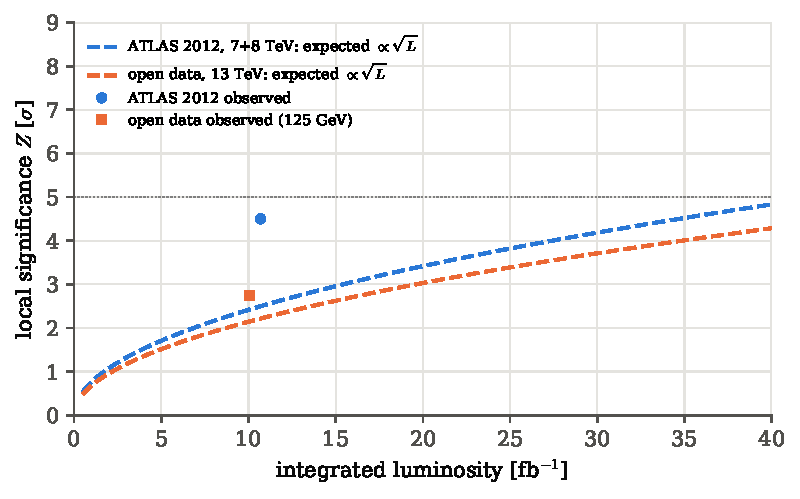
\includegraphics[width=0.85\linewidth]{figures/ch13/hyy_atlas2012.pdf}
\caption{The expected local significance of the diphoton search against integrated
luminosity, for the 2012 ATLAS analysis (blue dashed, scaled from its quoted $2.5\sigma$ at
$10.7\,\mathrm{fb}^{-1}$) and for ours (orange dashed, from $\HyyZexpOneTwoFive\sigma$ at
$10.06\,\mathrm{fb}^{-1}$), both growing as $\sqrt L$. The points are the observed local
significances. Both observations lie above their expectation: in 2012 by two units of $Z$, in our data
by about half a unit.}
\label{13d:fig:atlas2012}
\end{figure}

\subsection{Why they differ}
\label{13d:sec:repro-why}

Each ingredient of \eqref{13d:eq:repro} can be compared separately, and the formula says
how much each one matters: $Z\propto\sqrt{1-\rho^2}\,S/\sqrt{\sigma\beta}$ for one
category. Compared at equal luminosity, ours over theirs, one factor at a time:
\begin{itemize}[itemsep=2pt,leftmargin=1.2em]
  \item \emph{More Higgs bosons per $\mathrm{fb}^{-1}$: a factor
        $\HyyOurSperL/\HyyAtlasSperL=2.22$.} At $13\,$TeV the cross section times branching
        ratio of all four production modes together is $\HyyOurXS\,$fb, $\HyyXSratio$ times
        that at $7$--$8\,$TeV (gluon fusion alone is $102\,$fb, \cref{T4a:sec:higgs-lesson}),
        because at a higher energy a Higgs boson of fixed mass needs gluons carrying a
        smaller fraction of the proton's momentum, and such gluons are more numerous
        (\cref{ch:T4}). Our selection keeps a fraction $\HyyOurEff$ of the produced
        diphoton decays against ATLAS's $\HyyAtlasEff$ (they quote about $40\%$
        \srcref{AadHiggs2012}{\S5.4}), which takes back a little.
  \item \emph{More background per $\mathrm{fb}^{-1}$: a factor
        $(\HyyOurBetaPerL/\HyyAtlasBetaPerL)^{-1/2}=0.78$.} The diphoton continuum grows with
        energy as well, and the open-data photons pass a looser isolation: the calorimeter
        energy is summed in a cone of $\Delta R<0.2$ and compared with $6.5\%$ of $p_T$,
        where the 2012 analysis used a cone of $0.4$ and a fixed $4\,$GeV
        \srcref{AadHiggs2012}{\S5.1}, and a smaller cone lets more jets that fake photons
        through.
  \item \emph{A wider peak: a factor $(\HyyCBsig/\HyyAtlasSigma)^{-1/2}=0.82$.} Our width
        is what the released simulation gives; the release does not document the photon
        energy calibration in enough detail to trace the difference further.
  \item \emph{No categories: a factor $\HyyAtlasZincl/\HyyAtlasZcat=0.85$.} The ten
        categories raised ATLAS's leading-order $Z$ by separating the few events with a
        narrow peak and little background from the many with a wide peak and much
        background, exactly as \eqref{13d:eq:split} promises.
  \item \emph{A more flexible background: a factor
        $\sqrt{\HyyOurKeepGauss/\HyyAtlasKeep}=0.77$.} A degree-five polynomial over
        $55\,$GeV against a degree-four one over $60\,$GeV, and a wider peak that the
        polynomial imitates more easily (\cref{13d:sec:spurious}).
\end{itemize}
The product is $2.22\times0.78\times0.82\times0.85\times0.77=0.93$. The two predictions of
\eqref{13d:eq:repro} per unit of luminosity, $\HyyOurZpred/\sqrt{10.06}=0.70$ against
$\HyyAtlasZpred/\sqrt{10.7}=0.75$, are in exactly that ratio, and so, to the precision of
the formula, are the quoted expectations. The budget explains the opening puzzle: the
higher energy more than doubled the signal, and four smaller losses, each between $15$ and
$25\%$, took all of it back. The two largest, the background function and the
background density, are the cheapest to recover: categories with less background and a
narrower peak would improve both.

The \emph{observed} values differ for a different reason. ATLAS's diphoton excess was a
$\HyyAtlasMuPull\sigma$ upward fluctuation of the signal on top of an expected
$2.5\sigma$; ours is a fluctuation of about half a standard deviation.

\paragraph{The lesson.}
Reading the paper gives one number, $2.5\sigma$ expected; rebuilding it shows that the
number is the product of five ingredients, each of which can be measured separately and
traded against the others: signal per luminosity, background density under the peak,
mass resolution, how finely the events are sorted by their quality, and how flexible the
background function has to be. A resonance search
is designed by improving the weakest of these, and the formula
$Z^2\approx(1-\rho^2)\sum_cS_c^2/(2\sqrt\pi\sigma_c\beta_c)$ tells which one that is before
any data are taken.
\section{The full analysis, and what our shortcuts cost}
\label{13d:sec:nerfs}

Every number of this search came from a laptop-sized computation: $1.9\,$GB of files read
once, a few thousand toy spectra fitted by Newton's method, and each script ran within
minutes on four cores. The statistics is the same as in the collaboration's analysis, but
several pieces were simplified. Each simplification has a cost we can name, and for most
of them the cost was measured along the way.

\begin{center}
\small
\begin{tabular}{@{}>{\raggedright\arraybackslash}p{2.3cm}>{\raggedright\arraybackslash}p{4.3cm}>{\raggedright\arraybackslash}p{4.3cm}@{}}
\toprule
 & full analysis & ours, and the cost\\\midrule
events & all channels, full photon calibration, many times more data in later years & $10\,\mathrm{fb}^{-1}$ of released data, diphoton only; $Z\propto\sqrt L$ (\cref{13d:fig:atlas2012})\\
categories & ten in 2012, more later, each with its own background function & one (two as an example); the ten categories were worth $\HyyAtlasZincl\to\HyyAtlasZcat$ in 2012\\
signal shape & Crystal Ball plus Gaussian, simulated at many masses & Crystal Ball at $125\,$GeV, scaled to other masses; $\mu$ away from $125\,$GeV relative to a fixed yield\\
background choice & spurious-signal test on large simulated background samples & truths fitted to the same data (\cref{13d:sec:spurious}); the test only compares families\\
nuisance parameters & dozens: each efficiency, energy scale and resolution term, theory & four, with sizes taken from 2012 and from the release\\
toys & full fits with all nuisance parameters, auxiliary measurements redrawn & statistical part only, linear fits; nuisances changed $Z$ by less than $0.01$ here\\
global significance & Gross--Vitells in mass (and width), combined channels & Gross--Vitells in mass, checked with $\HyyToyNbkg$ toys\\
\bottomrule
\end{tabular}
\end{center}

\paragraph{Verification and research.}
Two kinds of simulation appeared in this search, and they did different jobs. The toys of
\cref{13d:sec:asym-check,13d:sec:cls-toys} \emph{verified} known analytic results: the
half-$\chi^2$ law of $q_0$, the Asimov median, the asymptotic CL$_s$. With $76\,000$ events
the formulas passed, so the toys added confidence but no new number. The background-only
scans of \cref{13d:sec:global} were the \emph{research instrument}: no closed formula
gives the global p-value of a scan over a fitted, bending background, and the
Gross--Vitells formula itself needs the upcrossing count that only simulated scans
provide. The same division runs through every capstone of this chapter: simulation checks
a formula where one exists and replaces it where none does.

\begin{recap}
\begin{itemize}[itemsep=1pt,leftmargin=1.2em]
  \item From the released 13 TeV files, the HyyAnalysis selection keeps $\HyyNData$ photon
        pairs in $105$--$160\,$GeV, where a Standard Model Higgs boson would add
        $\HyySigExp$ events; the invariant mass $2p_{T1}p_{T2}[\cosh\Delta\eta-\cos\Delta\phi]$
        is where it would appear as a peak.
  \item The signal is a Crystal Ball of width $\HyyCBsig\,$GeV fitted to weighted
        simulation; the background a fifth-order Bernstein polynomial, the least
        flexible family whose spurious signal stays below $20\%$ of the statistical error.
        Flexibility costs a fraction $\rho^2$ of $q_{0,\rm A}$, here more than half.
  \item The expected significance of a peak is
        $Z^2\approx(1-\rho^2)\sum_cS_c^2/(2\sqrt\pi\sigma_c\beta_c)$, and its mass precision
        $\sigma_m=\sqrt2\,\sigma/Z$; splitting into categories never loses, by
        $(S_1B_2-S_2B_1)^2/(B_1B_2(B_1+B_2))$.
  \item The data show a local $\HyyZloc\sigma$ excess at $\HyyMmax\,$GeV where
        $\HyyZexpOneTwoFive\sigma$ was expected at $125\,$GeV; toys confirm the asymptotic
        laws, and the global significance over $110$--$150\,$GeV is about
        $\HyyZgvObs\sigma$, with a trials factor of $\HyyTrialsObs$ and a background
        bump of similar local size at $\HyyMsecond\,$GeV.
  \item $\hat\mu=\HyyMuHat\pm\HyySigStat\,(\text{stat})\pm\HyySigSyst\,(\text{syst})$ and
        $\hat m_H=\HyyMhat\pm\HyyMhatLo\,$GeV, the mass error dominated by the photon
        energy scale.
  \item CL$_s$ excludes a signal of the Standard Model size at \HyyExclRanges\,GeV and
        not near $125\,$GeV, where the observed limit is $\HyyLimObsOneTwoFive$ against an
        expected $\HyyLimExpOneTwoFive$.
  \item Rebuilt from its Table 4, the 2012 ATLAS expected $2.5\sigma$ follows from the same
        formula; our larger signal per $\mathrm{fb}^{-1}$ is outweighed by more background,
        a wider peak, the absence of categories and a more flexible background function.
\end{itemize}
\end{recap}

\section*{Reading the literature}
\addcontentsline{toc}{section}{Reading the literature}
\label{13d:sec:literature}

\begin{itemize}[itemsep=2pt,leftmargin=1.2em]
  \item \emph{The CMB power spectrum on the real sky.} The \textit{Planck} 2018
        overview, power-spectrum and parameter papers \cite{Planck2018I,Planck2018V,Planck2018VI};
        the MASTER method \cite{Hivon2002}; the pseudo-$C_\ell$ and likelihood
        approximations of \cite{Efstathiou2004,HamimecheLewis2008}; a modern
        pseudo-$C_\ell$ code and its conventions \cite{Alonso2019}; HEALPix
        \cite{Gorski2005}; CAMB \cite{CAMB2000}.
  \item \emph{Topology of the real CMB sky.} \textit{Planck} 2018 isotropy and statistics
        \cite{Planck2018VII}; Minkowski functionals on the sphere
        \cite{SchmalzingGorski1998}; Betti numbers of the CMB \cite{Pranav2017}; the
        bias of an inverted simulated covariance \cite{Hartlap2007}.
  \item \emph{Galaxy clustering on a real survey.} The BOSS DR12 catalogues and weights
        \cite{Reid2016}; the systematics behind the weights \cite{Ross2012}; the
        first CMASS detection \cite{Anderson2012}; the DR12 correlation-function
        BAO \cite{Cuesta2016} and the final BOSS distances \cite{Alam2017}; the
        estimator \cite{LandySzalay1993} and weights \cite{FKP1994}; the first
        detection \cite{Eisenstein2005}; DESI's analysis with blinding
        \cite{DESI2024VI}; jackknife errors \cite{EfronStein1981,Norberg2009}.
  \item \emph{A Higgs search on collider open data.} The discovery papers
        \cite{AadHiggs2012,ChatrchyanHiggs2012}, of which the ATLAS one documents the
        diphoton categories, background functions and spurious-signal test in detail;
        the 13 TeV open-data release and its samples
        \cite{ATLASOpenData2020,SerkinOpenData2020}; the asymptotic formulas for $q_0$,
        $\tilde q_\mu$ and the Asimov data set \cite{Cowan2011} and the structure of the
        likelihood with constraint terms \cite{Cranmer2015}; the look-elsewhere effect
        and upcrossings \cite{GrossVitells2010}; the CL$_s$ method
        \cite{Junk1999,Read2002}.
\end{itemize}

\section*{Chapter summary}
\addcontentsline{toc}{section}{Chapter summary}
\label{13d:sec:chapter-summary}

Each capstone analysis runs the full pipeline on real data: a physical model, a field,
catalogue or list of events, a summary, its sampling distribution, and an inference. The
CMB power spectrum, the topology of the CMB sky, the clustering of CMASS galaxies and the
diphoton search differ in what is observed and what is undone, and share the last three
stages (\cref{13d:fig:chapter-map}). In the first three the summary is a curve or a set of
numbers and the question is a parameter or a consistency test; in the Higgs search the
summary is a histogram and the question is first a test (is there a peak?), then a
measurement (how strong, where?), then an exclusion (where is there none?), all from one
likelihood.

\begin{figure}[htbp]
\centering
\begin{tikzpicture}[
  box/.style={draw=black!50,rounded corners=2pt,fill=formblue!6,font=\footnotesize,
              align=center,minimum height=1.2cm,text width=2.05cm,inner sep=2pt},
  arr/.style={->,black!60}]
  \foreach \y/\a/\b/\c/\d/\e in {
     0/{\textit{Planck} map}/{mask, pseudo-$C_\ell$, MASTER}/{binned $C_\ell$}/{simulated covariance}/{$A_s$, $n_s$ by MCMC},
    -1.6/{\textit{Planck} map}/{degrade, cut sphere}/{Minkowski, Betti,\\persistence}/{Gaussian skies}/{$\chi^2$ and $p$-value},
    -3.2/{CMASS catalogue}/{positions, weights}/{$\hat\xi_0(s)$, Landy--Szalay}/{jackknife covariance}/{$\alpha$, $D_V/r_d$},
    -4.8/{ATLAS open data}/{selection, $m_{\gamma\gamma}$}/{mass histogram, $q_0$, $\tilde q_\mu$}/{asymptotics, toys}/{$Z$, $\hat\mu$, CL$_s$ limits}} {
    \node[box] (a) at (0,\y) {\a};
    \node[box] (b) at (2.6,\y) {\b};
    \node[box] (c) at (5.2,\y) {\c};
    \node[box] (d) at (7.8,\y) {\d};
    \node[box] (e) at (10.4,\y) {\e};
    \draw[arr] (a) -- (b); \draw[arr] (b) -- (c); \draw[arr] (c) -- (d); \draw[arr] (d) -- (e);
  }
  \foreach \x/\t in {0/data,2.6/observation undone,5.2/summary $S$,7.8/$P(S\given\theta)$,10.4/inference}
    \node[font=\scriptsize,black!70] at (\x,0.85) {\t};
\end{tikzpicture}
\caption{The four capstone analyses as rows of one pipeline: the CMB power spectrum
(top), the topology of the CMB sky, the clustering of CMASS galaxies, and the diphoton
Higgs search (bottom). Each column is one stage of the pipeline.}
\label{13d:fig:chapter-map}
\end{figure}

\begingroup
\small\sloppy
\renewcommand{\arraystretch}{1.25}
\begin{xltabular}{\linewidth}{@{}>{\raggedright\arraybackslash}p{2.6cm}
  >{\raggedright\arraybackslash}X >{\raggedright\arraybackslash}p{2.5cm}@{}}
\toprule
\textbf{concept} & \textbf{operational meaning} & \textbf{used later in}\\
\midrule
\endfirsthead
\toprule
\textbf{concept} & \textbf{operational meaning} & \textbf{used later in}\\
\midrule
\endhead
\multicolumn{3}{@{}l}{\emph{The CMB power spectrum of the real sky}}\\
masked, apodised map & multiply the map by a smooth mask that hides the Galaxy and point sources (\cref{8b:sec:apodisation}) & \cref{ch:14}\\
pseudo-$C_\ell$ and MASTER & the masked sky's spectrum is $\sum_{\ell'}M_{\ell\ell'}C_{\ell'}$; invert the binned coupling matrix (\cref{8b:sec:master}) & \cref{13c:sec:window}, \cref{ch:14}\\
beam and pixel window & divide the spectrum by $b_\ell^2p_\ell^2$ (\cref{8a:sec:beam}) & \cref{13b:sec:degrade}\\
simulated covariance & push Gaussian skies of the fiducial model through the same mask and noise (\cref{ch:08}) & \cref{13b:sec:hartlap}\\
reduced parameter fit & sample $(A_s,n_s)$ with the Metropolis--Hastings sampler of \cref{ch:09} & \cref{ch:14}\\
\midrule
\multicolumn{3}{@{}l}{\emph{The topology of the real CMB sky}}\\
one sky as one draw & test the sky against the simulated distribution of the Gaussian null (\cref{13b:sec:question}) & \cref{ch:14}\\
degrading a map & multiply $\alm$ by $b^{\rm new}_\ell p^{\rm new}_\ell/(b^{\rm old}_\ell p^{\rm old}_\ell)$ (\cref{13b:sec:degrade}) & \\
functionals on a cut sphere & area, boundary length and $V-E+F$ inside the mask (\cref{13b:sec:estimators}) & \cref{ch:14}\\
Mahalanobis $\chi^2$ and Hartlap & quadratic form of the statistics with a simulated covariance, its inverse rescaled (\cref{13b:sec:mahalanobis,13b:sec:hartlap}) & \cref{13c:sec:jk-bias}\\
rank $p$-value & fraction of simulations at least as extreme, with error $\sqrt{p(1-p)/n}$ (\cref{13b:sec:verdict}) & \cref{13d:sec:global}, \cref{ch:14}\\
Betti numbers and persistence on the sphere & $\beta_1=\beta_0-\chi$ on a cut sphere; $H_0$ diagrams compared by $W_1$ (\cref{13b:sec:betti}) & \cref{13c:sec:nerfs}\\
\midrule
\multicolumn{3}{@{}l}{\emph{Galaxy clustering of CMASS South}}\\
positions from $(\mathrm{RA},\mathrm{Dec},z)$ & comoving distance of the fiducial model, then Cartesian coordinates (\cref{13c:sec:positions}) & \cref{13c:sec:repro-equation}\\
catalogue weights & $w_{\rm tot}=w_{\rm systot}(w_{\rm cp}+w_{\rm noz}-1)$ for galaxies, times $w_{\rm FKP}$; randoms carry $w_{\rm FKP}$ (\cref{13c:sec:weights}) & \cref{ch:14}\\
window in pair counts & $\langle DD\rangle/\langle RR\rangle=1+\xi(s)$ in each thin shell (\cref{13c:sec:window}) & \cref{ch:14}\\
leave-one-region-out counts & $C_{-k}=C-C(k,\cdot)-C(\cdot,k)+C(k,k)$ (\cref{13c:sec:leave-one-out}) & \cref{13c:sec:jackknife}\\
jackknife covariance & $\frac{N-1}{N}\sum_k(\hat{\bm\xi}_{-k}-\bar{\bm\xi})(\cdots)\T$; exact for a mean, biased upward otherwise (\cref{13c:sec:jackknife}) & \cref{ch:14}\\
$\alpha$ to a distance & $D_V/r_d=\alpha\,D_V^{\rm fid}/r_d^{\rm tmpl}$, with $h$ cancelling (\cref{13c:sec:repro-equation}) & \cref{ch:14}\\
detection and location & $\sqrt{\Delta\chi^2}$ for existence, rise of $\chi^2(\alpha)$ for position; $\sigma_\alpha\sqrt{\Delta\chi^2}$ fixed by the bump's shape (\cref{13c:sec:repro-side,13c:sec:repro-why}) & \cref{13d:sec:mass}, \cref{ch:14}\\
subset against parent sample & $\Var(\alpha_S-\alpha_{NS})=\sigma_S^2-\sigma_{NS}^2$ (\cref{13c:sec:repro-why}) & \cref{ch:14}\\
\midrule
\multicolumn{3}{@{}l}{\emph{A Higgs search on collider open data}}\\
invariant mass & $m_{\gamma\gamma}^2=2p_{T1}p_{T2}[\cosh\Delta\eta-\cos\Delta\phi]$ from the stored photon momenta (\cref{13d:sec:data}) & \cref{ch:14}\\
weighted simulation & each selected simulated event stands for $L\sigma w_j\mathrm{SF}_j/\sum_kw_k$ real events (\cref{13d:sec:data}) & \cref{13d:sec:signal-shape}\\
Crystal Ball line shape & Gaussian core joined with equal value and slope to a power-law tail; tail area $\frac{n}{\alpha(n-1)}e^{-\alpha^2/2}$ (\cref{13d:sec:signal-shape}) & \cref{13d:sec:likelihood}\\
spurious signal & fit a background-only truth with candidate background plus signal; keep the families inventing less than $20\%$ of $\sigma_S$ (\cref{13d:sec:spurious}) & \cref{13d:sec:likelihood}\\
price of flexibility & fitted background parameters keep $1-\rho^2=1/(F_{\mu\mu}(\Fish^{-1})_{\mu\mu})$ of $q_{0,\rm A}$ (\cref{13d:sec:spurious}) & \cref{13d:sec:expected,13d:sec:repro}\\
expected significance of a peak & $q_{0,\rm A}\approx\sum_is_i^2/b_i\approx S^2/(2\sqrt\pi\sigma\beta)$ (\cref{13d:sec:expected}) & \cref{13d:sec:repro}, \cref{ch:14}\\
local and global significance & $Z_{\rm loc}=\sqrt{q_0}$; $p_{\rm glob}\approx p_{\rm loc}+\E[N(c_0)]e^{-(c-c_0)/2}$ from $100$ toys (\cref{13d:sec:scan,13d:sec:global}) & \cref{ch:14}\\
profile-likelihood measurement & crossings of $-2\ln\lambda=1$; systematic part $\sqrt{\sigma_{\rm tot}^2-\sigma_{\rm stat}^2}$ (\cref{13d:sec:mu}) & \cref{ch:14}\\
mass precision & $\sigma_m=\sqrt2\,\sigma/Z$ for a Gaussian peak (\cref{13d:sec:mass}) & \cref{13d:sec:repro}\\
categories & $q_0$ adds over independent spectra; splitting gains $(S_1B_2-S_2B_1)^2/(B_1B_2(B_1+B_2))$ (\cref{13d:sec:categories}) & \cref{13d:sec:repro}\\
CL$_s$ limits and the Brazil band & $\mathrm{CL}_{s+b}/\mathrm{CL}_b<0.05$; band $\sigma_{\rm A}[N+\Phi^{-1}(1-\alpha\Phi(N))]$ from the background-only Asimov set (\cref{13d:sec:limits}) & \cref{ch:14}\\
\bottomrule
\end{xltabular}
\endgroup
  